\NeedsTeXFormat{LaTeX2e}[1996/06/01]
 \documentclass{book}
 \usepackage{natbib}
 \usepackage[figuresright]{rotating}
 \usepackage{floatpag}
 \rotfloatpagestyle{empty}
 \usepackage{mathrsfs}
 \usepackage{xspace}
 \usepackage{amsthm,amsmath}
 \usepackage{graphicx} 
 \usepackage{mathtools}
 \usepackage{txfonts}
 \usepackage{multind}
 \usepackage[breaklinks,hidelinks]{hyperref} 
 \usepackage{color}
 \usepackage{listings}
%	this is for delayed exercises, I don't use it now
%   \usepackage[lastexercise,answerdelayed]{exercise}
 \usepackage[all]{xy}
 \usepackage{alltt}
 \usepackage[shortlabels]{enumitem}
 \makeatletter
\newcommand{\customlabel}[2]{%
  \protected@edef\@currentlabel{#1}% Set the custom label
  \label{#2}% Define the label
}
\makeatother
 \usepackage{mik-makro}
\usepackage{tikz-cd}
\usepackage{libertine}
\usepackage{inconsolata}

% knowledge stuff
\input{knowledge-config}

 \makeindex{authors}
 \makeindex{subject} 
 \makeglossary 
 \theoremstyle{plain}% default
 \newtheorem{theorem}{Theorem}[chapter]
 \newtheorem{lemma}[theorem]{Lemma}
 \newtheorem{claim}[theorem]{Claim} 
 \newtheorem{proposition}[theorem]{Proposition}
 \newtheorem{corollary}[theorem]{Corollary}
 \newtheorem{conjecture}[theorem]{Conjecture}
 \newtheorem*{theorem*}{Theorem}
 \newtheorem*{lemma*}{Lemma} 
 \newtheorem*{proposition*}{Proposition}
 \newtheorem*{corollary*}{Corollary}
 \newtheorem*{conjecture*}{Conjecture}
 \theoremstyle{definition}
 \newtheorem{definition}[theorem]{Definition}
 \newtheorem{example}[theorem]{example}
 \newtheorem{prob}[theorem]{Problem}
 \newtheorem{remark}[theorem]{Remark}
 \newtheorem{notation}[theorem]{Notation}
 \newtheorem{exer}[theorem]{Exercise}
 \newtheorem*{definition*}{Definition}
 \newtheorem*{example*}{myexample}
 \newtheorem*{prob*}{Problem}
 \newtheorem*{remark*}{Remark}
 \newtheorem*{notation*}{Notation}
 \newtheorem*{exer*}{Exercise}
 \setcounter{tocdepth}{2}



%  If I use the cambridge style, then I need extra macros
% if I don't these should be commented out
\newcommand{\ifcambridge}[1]{

}
% this is the book version, so the exercises are small and the solutions are not given 

\newcommand{\mikexercise}[2]{
	{\small
\begin{mexercise} 
	#1 
\end{mexercise}
	}
}


% Define custom settings for code listings
\lstset{
    basicstyle=\ttfamily\footnotesize, % Code font and size
    % keywordstyle=\color{blue}\bfseries, % Keywords in bold blue
    commentstyle=\color{gray}, % Comments in gray
    stringstyle=\color{red}, % Strings in red
    numbers=left, % Line numbers on the left
    numberstyle=\tiny\color{gray}, % Line number style
    stepnumber=1, % Line number step
    numbersep=5pt, % Space between line numbers and code
    backgroundcolor=\color{lightgray!20}, % Light gray background
    % frame=single, % Frame around the code
    tabsize=4, % Tab size
    breaklines=true, % Line breaking
    captionpos=b, % Caption position (bottom)
    language=Python, % Default language
    mathescape=true, % Allow math mode in code
    escapechar=|,
    aboveskip=10pt, % Space above the listing
    belowskip=10pt,  % Space below the listing
    xleftmargin=15pt, % Left margin inside the box
    xrightmargin=15pt % Right margin inside the box
}

 \begin{document}
 \newcommand{\decisionproblem}[2]
{
	\begin{itemize}
		\item {\bf Input.} #1
		\item {\bf Output.} #2
	\end{itemize}
}

\newcommand{\freevar}[1]{\mathrm{var}(#1)}

\newcommand{\fdp}{\textsc{fdp}\xspace}

\newcommand{\pspace}{{\sc{PSpace}\xspace}}
\newcommand{\indvec}[1]{\atoms^{\langle #1 \rangle}}
 \newcommand{\dimension}[1]{\mathrm{dim}(#1)}
\newcommand{\leastsup}[1]{\mathrm{sup}(#1)}

\newcommand{\syntdim}[1]{\mathrm{dim}(#1)}
\newcommand{\syntsize}[1]{|#1|}
\newcommand{\semdim}[1]{\mathrm{\red{dim}}(#1)}
\newcommand{\semsize}[1]{\red|#1\red|}

\newcommand{\orbitsize}[2]{|#1|_{#2}}
%\newcommand{\saut}[1]{\mathrm{G}_{#1}}
%\newcommand{\aut}{\mathrm{G}}
%\newcommand{\secfm}{\bfseries{\scshape{fm\ }}}
%\newcommand{\fm}{\textsc{fm}\ }
%\newcommand{\tneq}{\(\neq\)}
\newcommand{\tleq}{\(\leq\)}
% \newcommand{\tin}{\(\in\)}
% \newcommand{\tnotin}{\(\notin\)}
% \newcommand{\tcup}{\(\cup\)}
% \newcommand{\temptyset}{\(\emptyset\)}
% \newcommand{\tcap}{\(\cap\)}
% \newcommand{\ttimes}{\(\times\)}

\newcommand{\approxi}[2]{#1^{(#2)}}

\newcommand{\cellc}[2]{\mathsf{cell}_{#1}(#2)}
\newcommand{\tatoms}{\(\ \!\!\!\!\atoms\)}

% \newcommand{\booltrue}{\ensuremath{\mathtt{true}}}
% \newcommand{\boolfalse}{\ensuremath{\mathtt{false}}}
\newcommand{\tset}[1]{\{#1\}}

\newcommand{\settype}{\mathtt{set}}
\newcommand{\atomtype}{\mathtt{atom}}

\newcommand{\red}[1]{{\color{red}#1}}
\newcommand{\blue}[1]{{\color{blue}#1}}

\newcommand{\exercisepart}{

\bigskip

{\noindent \large \bf Exercises}


}
\newcommand{\setexpr}[3]{\set{#1\ |\ \text{ for }#2 \in \atoms \text{ such that }#3}}
\newcommand{\setexprtup}[4]{\set{#1\ |\ \text{ for }#2 \in \atoms^{#3} \text{ such that }#4}}
\newcommand{\setexprtrue}[2]{\set{#1\ |\ \text{ for }#2 \in \atoms}}
\newcommand{\setexprtuptrue}[3]{\set{#1\ |\ \text{ for }#2 \in \atoms^{#3}}}

\newcommand{\symbolpushbis}[2]{\symbolpush{#1 \ : \ #2}}
\newcommand{\symbolpush}[1]{\underline{#1}}

\newcommand{\aequiv}[1]{\stackrel{#1}\sim}
\newcommand{\locations}{\mathsf{Loc}}

\newcommand{\bibnotes}[1]{
\bigskip
{\footnotesize
\noindent {\bf Bibliographic notes for Section~\arabic{section}. }
#1}
}

% these two macros are for delayed exercises, I don't use them now
% \renewcommand{\ExerciseHeader}{\noindent \textbf{\ExerciseName~\ExerciseHeaderNB\ExerciseHeaderTitle
% \ExerciseHeaderOrigin. }}
% \renewcommand{\AnswerHeader}{\noindent {\textbf{Solution to \ExerciseName\ \ExerciseHeaderNB.\\}}}

\newcounter{exercisecounter}
\newenvironment{mexercise}{
\refstepcounter{exercisecounter}

\smallskip\noindent{\textbf{{Exercise \arabic{exercisecounter}. }}}}{
}






\newcommand{\pv}[1]{{\mathtt{#1}}}

% the original picture files, from illustrator
\newcommand{\mypic}[1]{
\begin{center}
	\includegraphics[page=#1,scale=0.5]{pictures/from-ai}
\end{center}
}

% for pictures with figma
\newcommand{\mypicb}[1]{
\begin{center}
	\includegraphics[page=#1,scale=0.22]{pictures/atom-book}
\end{center}
}

%\newcommand{\notin}{\not \in}

\newcommand{\sets}{\mathsf{set}}
\newcommand{\setbuil}{\mathsf{setbuil}}
\newcommand{\defset}{\mathsf{hdef}}
\newcommand{\hofset}{\mathsf{hof}}

\newcommand{\setbuild}[2]{\set{\ #1 \ | 
\begin{tabular}{l}
	#2
\end{tabular}}}

% the tabular in the above macro can make it too wide, hence this one
\newcommand{\setbuildoneline}[2]{\set{\ #1 \ | 
\text{ #2}\ }}

\newcommand{\myunderbrace}[2]{\underbrace{#1}_{\mathclap{\text{\scriptsize 
\begin{tabular}{c}
	#2
\end{tabular} }}}}
\newcommand{\myoverbrace}[2]{\overbrace{#1}^{\mathclap{\text{\scriptsize 
\begin{tabular}{c}
	#2
\end{tabular} }}}}

\newcommand{\Bool}{2}
\newcommand{\eve}{\text{Eve}}
\newcommand{\adam}{\text{Adam}}
\newcommand{\john}{\text{John}}
\newcommand{\tom}{\text{Tom}}
\newcommand{\jim}{\text{Jim}}
\newcommand{\mary}{\text{Mary}}

\newcommand{\deflift}{{\mathsf{def}}}
\newcommand{\tti}{{\mathtt I}}
\newcommand{\ttj}{{\mathtt J}}
\newcommand{\qatom}{(\mathbb Q, <)}
\newcommand{\sem}[1]{[\![#1]\!]}
\newcommand{\fraisse}{Fra\"iss\'e } 

\newcommand{\saut}[1]{\mathrm{G}_{#1}}
\newcommand{\aut}{\mathrm{G}}
\newcommand{\secfm}{\bfseries{\scshape{fm\ }}}
%\newcommand{\fm}{\textsc{fm}\ }
\newcommand{\tneq}{\(\neq\)}
\newcommand{\tin}{\(\in\)}
\newcommand{\tnotin}{\(\notin\)}
\newcommand{\tcup}{\(\cup\)}
\newcommand{\temptyset}{\(\emptyset\)}
\newcommand{\tcap}{\(\cap\)}
\newcommand{\ttimes}{\(\times\)}

\newcommand{\structclass}{\mathscr A}
\newcommand{\structclassb}{\mathscr B}
\newcommand{\structclassh}{\mathscr H}
\newcommand{\structa}{\mathbb A}
\newcommand{\structb}{\mathbb B}
\newcommand{\structc}{\mathbb C}
\newcommand{\structh}{\mathbb H}

\newcommand{\atoms}{\mathbb A}
\newcommand{\field}{\mathbb F}
\newcommand{\universe}[1]{\mathrm{universe(#1)}}
\newcommand{\Fff}{\mathscr F}
\newcommand{\limmodel}{\underline \structa}
\newcommand{\arity}{\mathrm{arity}}
\newcommand{\lincomb}{\mathrm{Lin}}
\newcommand{\length}{\mathrm{len}}

% various kinds of function spaces
\newcommand{\lineqfun}[2]{ #1 \underset{\text{lineq}}{\longrightarrow} #2}
\newcommand{\linfsfun}[2]{ #1 \underset{\text{linfs}}{\longrightarrow} #2}
\newcommand{\eqfun}[2]{ #1 \underset{\text{eq}}{\longrightarrow} #2}
\newcommand{\fsfun}[2]{ #1 \underset{\text{fs}}{\longrightarrow} #2}

\newcommand{\generate}[1]{\langle #1 \rangle}

\newcommand{\atoma}{{a}}
\newcommand{\atomb}{{b}}
\newcommand{\atomc}{{c}}
\newcommand{\atomd}{{d}}

\newcommand{\atomq}{{q}}
\newcommand{\atomzero}{{\underline 0}}
\newcommand{\atomone}{{\underline 1}}
\newcommand{\atomtwo}{{\underline 2}}
\newcommand{\atomthree}{{\underline 3}}

 
\newcommand{\atomseta}{{A}}
\newcommand{\atomsetb}{{B}}
\newcommand{\atomsetc}{{C}}
\newcommand{\atomsets}{{S}}
\newcommand{\atomsett}{{T}}

\newcommand{\Qfin}{Q_{\mathrm{fin}}}
\newcommand{\Afin}{A_{\mathrm{fin}}}

\newcommand{\bind}{\nabla}
\newcommand{\powerset}{{\mathsf P}}
\newcommand{\pfin}{{\mathsf P}_{\text{fin}}}
\newcommand{\decproblem}[3]
{\begin{center}
\fbox{
\begin{tabular}{rl}
\textsc{Problem}: & #1 \\
\textsc{Input}: & #2\\
\textsc{Output}: & #3
\end{tabular}
}
\end{center}}

\newcounter{openquestioncounter}
\newenvironment{openquestion}{
\medskip

\refstepcounter{openquestioncounter}
\smallskip\noindent{\textbf{{Open question \arabic{openquestioncounter}. }}}}{\hfill $\Box$
\medskip 
}







\newcommand{\eqdef}{\stackrel {\mathrm{def}} = }

\newcommand{\Ii}{\mathcal I} 

 \title 
 {Slightly Infinite Sets}
\author{Miko{\l}aj Boja\'nczyk\\[3\baselineskip]
\today \\ The latest version can be downloaded from:\\
 mimuw.edu.pl/$\sim$bojan/paper/atom-book 
 }
 \ifcambridge{
\bookabstract{This is the guide for authors who are preparing written,
 rather than edited, books.}}
\ifcambridge{\bookkeywords{\LaTeX; authored books; CUP style; cambridge7A.cls.}}
\frontmatter 
\maketitle
 
\tableofcontents
% \listofcontributors
\chapter*{Preface}

This book is about algorithms that run on objects that are infinite, but finite up to certain symmetries.
Under a suitably chosen notion of symmetry, such objects -- called \emph{orbit-finite sets} -- can be represented, searched and processed just like finite sets. The goal of the book is to explain orbit-finiteness and demonstrate its usefulness. Most of the examples of orbit-finite sets are taken from automata theory, since this is where orbit-finite sets began. 

\mainmatter 
 
 
\begin{scope}\knowledgeimport{equality}
\chapter{Polynomial orbit-finite sets}
\label{sec:pof-sets}

The general idea in this book is to discuss sets which are built from some basic infinite set $\atoms$, and which are simple enough to be represented finitely and manipulated algorithmically. These sets will be called \emph{orbit-finite sets}. The fully general notion will be described in Chapters~\ref{cha:orbit-finite-equality} and~\ref{ch:beyond-equality}, but we begin  the book with a special case, called \emph{"polynomial orbit-finite sets"}, which is simpler to formalize, and yet general enough to describe most interesting examples. 

For the first few chapters of this book, the  basic infinite set $\atoms$ that will be used to build the other sets will have no structure except equality. The idea of having ``no structure except equality'' will be formalized later on, by using invariance under "atom permutations". For the moment, this idea will be apparent in the examples, and our convention that elements of $\atoms$ -- which will be called \emph{atoms} -- are names such as John or Eve. Everybody knows that names have no structure beyond equality.

Before formally defining "polynomial orbit-finite sets", we begin with several examples. These  examples are based on automata theory, which was the original motivation for these notions.

\begin{myexample}\label{ex:pof-dfa}
    Consider the language 
    \begin{align*}
    \setbuildoneline{w \in \atoms^*}{\text{the first and last letters of $w$ are the same}}.
    \end{align*}
    To recognise this language, we use a deterministic automaton that remembers the first letter seen in its state, plus one extra bit of information that tells us whether the last letter seen is the same as the first. This state space  consists of an initial state, and two disjoint copies of the atoms. We write this state space as  follows, where $+$ is used to denote disjoint union:
    \begin{align*}
        \set{\text{initial}} 
        \quad + \quad 
        \myunderbrace{\atoms}{equal}
        \quad + \quad 
        \myunderbrace{\atoms}{nonequal}.
    \end{align*}
    There are two copies of the atoms: the ``equal'' copy and the ``nonequal'' copy. For an atom $a \in \atoms$, we write $\text{equal}(a)$ for its first copy, and $\text{nonequal}(a)$ for its second copy. The choice of copy corresponds to storing one bit of information.
    The  transition function of the automaton, which is a function because the automaton is deterministic, consists of the following transitions, where $a$ and $b$ range over~$\atoms$:
    \begin{align*}
    \text{initial}  & \stackrel a \to \text{equal}(a) \\
    \text{equal}(a) & \stackrel b \to
    \begin{cases}
        \text{equal}(a) & \text{if $a = b$} \\
        \text{nonequal}(a) & \text{if $a \neq b$}
    \end{cases}\\
    \text{nonequal}(a) & \stackrel b \to
    \begin{cases}
        \text{equal}(a) & \text{if $a = b$} \\
        \text{nonequal}(a) & \text{if $a \neq b$}.
    \end{cases}
    \end{align*}
    The accepting states are those from the first copy of $\atoms$. 
\end{myexample}

The automaton in the above example was deterministic. Here is an example of an automaton that is nondeterministic.
\begin{myexample}\label{ex:pof-nfa} 
    Consider the language 
        \begin{align*}
        L = \setbuild{w \in \atoms^*}{some letter appears  at least twice}.
        \end{align*}
        When it reads an input letter, the  recognizing  automaton uses nondeterminism to guess if this letter will appear a second time. It then loads that letter into its state, and waits for a second appearance, upon which it enters an accepting sink state. The state space is 
        \begin{align*}
            \set{\text{initial, accept}} 
            \quad + \quad 
            \atoms.
        \end{align*}
        The first two states are the initial and accepting states, respectively. 
        The transitions of this automaton are listed below, where $a$ and $b$ range over $\atoms$:
        \begin{align*}
        \text{initial} & \stackrel a \to \text{initial}\\
        \text{initial} & \stackrel a \to a \\
        a & \stackrel b  \to 
        \begin{cases}
            \text{accept} & \text{if $a = b$} \\
             a & \text{if $a \neq b$}
        \end{cases}\\
        \text{accept} & \stackrel a \to \text{accept}.
        \end{align*}
        The nondeterminism is in the first two kinds of transitions. When the automaton is in the initial state, and it sees a letter $a$, then it can choose to either remain in the initial state, to go to state $a$. The first choice is made if the automaton does not expect $a$ to appear again, otherwise the second choice is made.
        We will later show that this language cannot be recognised by a deterministic automaton, but this will require a formal definition of the model.
\end{myexample}

In the automata from the above examples, the state space could be infinite, but it had a very special form: each state would store some finite information (for example, is the state accepting or rejecting), and some atoms. So far, each state would store zero or one atom, but one could of course imagine that more atoms are stored, e.g.~we could have a state space of the form 
\begin{align*}
\atoms^0 + \atoms^0 + \atoms^1 + \atoms^7.
\end{align*}
As before, we write $+$ for disjoint union of sets. In the disjoint union above,  the  "components" of the form $\atoms^0$ represent states where no atoms are stored, such as the initial states in the two examples.  This leads us to the following definition.

\begin{definition}[Pof set]\label{def:pof-set}
    A ""polynomial orbit-finite set"", "pof set" for short, is any finite disjoint union 
    \begin{align*}
    \atoms^{d_1} + \cdots + \atoms^{d_k}
    \end{align*}
    for some $k,d_1,\ldots,d_k \in \set{0,1,\ldots}$. 
\end{definition}

It should be clear why we use the word ``polynomial'' in the name -- syntactically a "pof set" is the same thing as a univariate polynomial with coefficients in the natural numbers. The meaning of the words ``orbit-finite'' will become apparent later in this section, when we discuss "orbits" under the action of   "atom permutations". In a "pof set", we use the name ""component"" for summands in the disjoint union. The "pof set" in the above definition has $k$ component, and the $i$-th component is  $\atoms^{d_i}$. The ""dimension"" of a "component" is the exponent $d$, the "dimension" of a "pof set" is the maximal  "dimension" of its "components". 

In the first chapters of this book, we will be interested in computational models, such as automata or Turing machines, where instead of finite sets, we use "pof sets". We already saw this in Examples~\ref{ex:pof-dfa} and~\ref{ex:pof-nfa}, which used automata where the  state spaces and input alphabets were "pof sets". This resulting theory will generalize the standard theory of finite objects, because a finite set can be seen as a "pof set" of  "dimension" zero. For example, a set with three elements can be seen as a "pof set" 
\begin{align*}
\atoms^0 + \atoms^0 + \atoms^0
\end{align*}
that has three "components" of dimension zero. We use the notational convention where $1$ is the set $\atoms^0$, and therefore the above set can also be denoted as 
\begin{align*}
1 + 1 + 1.
\end{align*}
One can further streamline the notion, and write $3$ for this set, which is something that we will also sometimes do.

In order to get a meaningful theory,  we need to make some restrictions on the way that elements of "pof sets" are manipulated. Otherwise, we would be working with models that use countable sets instead of finite ones, and without further restrictions there is nothing interesting that can be said at this level of generality, at least as long as we care about computability. 

The restriction that we make formalizes the  notion that atoms have no structure beyond equality. The idea is that if atoms are renamed in a way that preserves equality, then  all properties should be preserved. For example, if an automaton has a transition of the form  
\begin{align*}
(\john, \eve) 
\quad \stackrel \adam \to \quad 
(\adam, \john)
\end{align*}
then the same automaton should also have a transition of the form 
\begin{align*}
    (\tom, \adam) 
    \quad \stackrel \john \to \quad 
    (\john, \tom),
    \end{align*}
because the equality patterns are the same in both transitions. This notion is formalized in the following definition, by using ""atom permutations"", which are  defined to be bijective functions of type $\atoms \to \atoms$. We use the convention that "atom permutations" are denoted by $\pi$ or $\sigma$. 

\begin{definition}[Equivariant subset]\label{def:equivariant-pof}   
    A subset $X \subseteq \atoms^d$ is called ""equivariant"" if it is stable under applying "atom permutations", i.e. 
    \begin{align*}
    (a_1,\ldots,a_d) \in X 
    \quad \Leftrightarrow \quad
    (\pi(a_1),\ldots,\pi(a_d)) \in X
    \end{align*}
    holds for every "atom permutation"  $\pi$. A subset of a "pof set" is called "equivariant" if its intersection with each "component" is "equivariant".
\end{definition}

\begin{myexample}[Orbits in $\atoms^3$]\label{ex:pof-orbits-3}
    Consider the set $\atoms^3$. Up to "atom permutations", this set contains five kinds of  elements, namely a non-repeating triple 
    \begin{align*}
    (\john,\eve,\tom),
    \end{align*}
    three kinds of triples that use two atoms 
    \begin{align*}
    (\john,\eve,\eve), \quad (\eve,\john,\eve), \quad (\eve,\eve, \john),
    \end{align*}
    and  a triple that uses the same atom three times 
    \begin{align*}
    (\john,\john,\john).
    \end{align*}
    These five elements represent all possible equality types that can arise in triples of atoms. Depending on its equality type,  every other element of $\atoms^3$ can be mapped to one of the above five example using an "atom permutation", and the five kinds are all different, i.e.~none of them can be mapped to another by an "atom permutation". If we want to choose an "equivariant" subset of $\atoms^3$, we need to decide for each of the five kinds whether we want to include it or not. The five decisions are independent, and therefore there are $2^5$ possibilities of choosing an "equivariant" subset. 
\end{myexample}

The kinds of elements, as described in the above example, will be called \emph{"orbits"}. This is because they are the special case of the general notion of "orbits" under a group action, in the case where the group is the  group of all "atom permutations". 

\begin{definition}
    [Orbit]\label{def:orbit-in-pof} The ""orbit"" of an element $x$ in a "pof set" $X$ is the set 
    \begin{align*}
    \setbuild{\pi(x)}{$\pi$ is an "atom permutation"}.
    \end{align*}
\end{definition}

\begin{myexample}[Orbits in $\atoms^d$]\label{ex:how-many-orbits-in-power-of-atoms}
    In Example~\ref{ex:pof-orbits-3}, we showed that the set $\atoms^3$ has five "orbits". More generally, the number of "orbits" in $\atoms^d$ is the number of equivalence relations on the set $\set{1,\ldots,d}$. This is because an orbit describes an equality type, i.e.~information about which coordinates in the tuple are equal to each other. Therefore, counting orbits in $\atoms^d$ is the same as counting equivalence relations on $\set{1,\ldots,d}$.  The number of such equivalence relations  is called the Bell number, and it grows exponentially with $d$. For example, the 4-th Bell number is 15, and the 5-th Bell number is 52.
\end{myexample}

In the above example, we have argued that for sets of the form $\atoms^d$, the number of "orbits"  is finite, albeit exponential. Since every "equivariant" set is a union of orbits, it follows that the number of "equivariant" subsets in $\atoms^d$ is also finite, albeit doubly exponential in the dimension $d$. These results extend immediately to "pof sets", which are finite disjoint unions of such sets. This is because the number of orbits in a disjoint union $X+Y$ is the sum of the numbers of orbits in the summands $X$ and $Y$.  Hence, we get the following result, which explains the expression ``orbit-finite'' in the name ``polynomially orbit-finite''.
\begin{lemma}\label{lem:pof-finitely-many-equivariant}
    Every "pof set" has finitely many "orbits", and finitely many "equivariant" subsets. 
\end{lemma}

The orbit count for a product $X \times Y$ is more subtle, and will be discussed later on. For example $\atoms^1$ has one orbit and $\atoms^2$ has two orbits, while their product $\atoms^3$ has five orbits, which shows that the formula cannot be completely trivial.


In Definition~\ref{def:equivariant-pof}, we defined "equivariant" subsets of one "pof set". This extends naturally to relations on "pof sets", e.g.~binary relations 
\begin{align*}
R \subseteq X \times Y,
\end{align*}
where $X$ and $Y$ are "pof sets". This is because the product of two "pof sets" can itself be seen as a new "pof set", by distributing products across disjoint unions:
\begin{align*}
(\sum_{i \in I} \atoms^{d_i})
\times 
(\sum_{j \in J} \atoms^{e_j})
\quad \equiv \quad 
\sum_{\substack{ i \in I \\ j \in J}} \atoms^{d_i + e_j}.
\end{align*}
Equivariant relations can also be described directly: a binary relation is equivariant if and only if  membership in it is stable under applying the same atom permutation to both coordinates:
\begin{align*}
(x,y) \in R 
\quad \Leftrightarrow \quad 
(\pi(x),\pi(y)) \in R
\qquad 
\text{for every atom permutation $\pi$.}
\end{align*}
The above discussion was for binary relations, but the same idea extends to relations of any finite arity.
Similarly, we can also talk about "equivariant" functions $f : X \to Y$. These are the same as binary relations that are both "equivariant" and functional, i.e.~for every input $x \in X$ there exactly one output $y \in Y$ such that $(x,y)$ belongs to the relation. 

\begin{myexample}[Functions with Boolean outputs]\label{ex:functions-with-boolean-outputs}
    To represent booleans, we can use the set $2$, which is the disjoint union $1+1$, where $1$ is defined to be the set $\atoms^0$. An element of the  set $2$ consists of one bit of information, and no atoms. Sets which are disjoint union of several copies of $1$ will be called ""atomless"", and they will correspond to the usual finite sets. For an atomless set, the action of atom permutations is trivial, i.e.~$\pi(x)=x$, since there are no atoms to change. 
For a "pof set" $X$, an "equivariant" function of type $X \to 2$ is the same thing as an "equivariant" subset of $X$. This is because, by triviality of the action on the output set, we have 
\begin{align*}
f(x) = y \quad \Leftrightarrow \quad f(\pi(x)) = y \qquad \text{for every $y \in 2$},
\end{align*}
which means that the function has the same outputs for every two inputs in the same orbit.
\end{myexample}

\begin{myexample}[Equivariant functions of type $\atoms \to \atoms$] In this example, we show that there is only one "equivariant" function of type $\atoms \to \atoms$, namely the identity. Clearly the identity is "equivariant", since the corresponding set of pairs is the diagonal 
    \begin{align*}
    \setbuild{(a,a)}{$a \in \atoms$},
    \end{align*}
    and this set is "equivariant". (It happens to be exactly one orbit.) Let us now prove that there is no other "equivariant" function of this type. Toward a contradiction,  suppose  that an "equivariant" function would map some input atom $a$ to an output atom $b \neq a$. From the pair $(a,b)$ we can go to any pair $(a,c)$ with $a \neq c$ by applying an "atom permutation". This would yield a violation -- in fact infinitely many violations -- of the functionality condition, which says that each input has only one output. 
\end{myexample}
\begin{myexample}[Equivariant functions of type $\atoms^2 \to \atoms$]
    \label{ex:equivariant-functions-of-type-atoms2-to-atoms}
    Let us list all "equivariant" functions of type $f : \atoms^2 \to \atoms$.  
    If the input to such a function is a repeating pair $(a,a) \in \atoms^2$, then the output has to be $a$, by the same argument as in the previous example. If the input is a non-repeating pair $(a,b)$ with $a \neq b$, then the output must be either the first argument $a$ or the second argument $b$, and it cannot be a fresh atom, again by the same argument as in the previous example. Furthermore, this choice must be uniform: if for some input that is a  non-repeating pair the output is the first coordinate, then this is true for all other inputs that are non-repeating pairs. This is because every non-repeating pair can be mapped to every other non-repeating pair by an "atom permutation". Therefore, there are two possibilities for $f$: it is either the projection to the first coordinate, or the projection to the second coordinate.
\end{myexample}

\begin{myexample}
    An example of an "equivariant" function of type $\atoms^3 \to \atoms$ is the following function, which projects onto the second or third coordinate, depending on whether the first two coordinates are equal or not:
    \begin{align*}
    (a,b,c) 
    \quad \mapsto \quad 
        \begin{cases}
            c & \text{if $a \neq b$} \\
            b & \text{if $a = b$}.
        \end{cases}
    \end{align*}
    Generally speaking, an "equivariant" function of type $\atoms^d \to \atoms$ will look at the equality type (i.e.~the orbit) of the input, and based on that orbit it will choose one of the input coordinates to be sent to the output. Therefore, the number of such functions is the product
    \begin{align*}
    \prod_X  \text{(number of distinct atoms in the orbit $X$)},
    \end{align*}
    where $X$ ranges over orbits in the set $\atoms^d$. 
\end{myexample}

As shown in Lemma~\ref{lem:pof-finitely-many-equivariant}, a "pof set" will have finitely many "equivariant" subsets. If $X$ and $Y$ are "pof sets", then the same will be true for $X \times Y$, and therefore there will be  finitely many "equivariant" relations $R \subset X \times Y$. Only some of these relations will be functions. Summing up, for every pair of "pof sets" $X$ and $Y$, there will be finitely many "equivariant" functions of type $X \to Y$.


\exercisepart
\mikexercise{\label{pof-one-way-permutation} In the definition of an equivariant subset from Definition~\ref{def:equivariant-pof}, we have an equivalence $\Leftrightarrow$, and we quantify over atom permutations, which can be briefly written as
\begin{center}
    \begin{tabular}{lllll}
        0.  & 
        $\bar a \in X$ & $\Leftrightarrow$ & $\pi(\bar a) \in X$ 
        & for all permutations $\pi : \atoms \to \atoms$.
    \end{tabular}
\end{center}
Instead of a two-way implication, we can have a one-way implication in either of the two directions, and we can quantify over functions that are not necessarily permutations, as in the following variants:
\begin{center}
    \begin{tabular}{lllll}
        1.  & 
        $\bar a \in X$ & $\Rightarrow$ & $\pi(\bar a) \in X$ 
        & for all permutations $\pi : \atoms \to \atoms$\\
        2.  & 
        $\bar a \in X$ & $\Leftarrow$ & $\pi(\bar a) \in X$ 
        & for all permutations $\pi : \atoms \to \atoms$\\
        3.  & 
        $\bar a \in X$ & $\Leftrightarrow$ & $\pi(\bar a) \in X$ 
        & for all functions $\pi : \atoms \to \atoms$\\
        4.  & 
        $\bar a \in X$ & $\Rightarrow$ & $\pi(\bar a) \in X$ 
        & for all functions $\pi : \atoms \to \atoms$\\
        5.  & 
        $\bar a \in X$ & $\Leftarrow$ & $\pi(\bar a) \in X$ 
        & for all functions $\pi : \atoms \to \atoms$
    \end{tabular}
\end{center}
Which variants are equivalent to the original definition, as in variant 0?}{ Variants 0,1,2 are equivalent to each other, and stronger than all  the other variants. Variant 3 is the weakest one, weaker than all the others. Finally, variants 4 and 5 are incomparable to each other, and set between 0=1=2 and 3. Here is a more detailed explanation:
    \begin{enumerate}
        \item     This variant, which uses an implication $\Rightarrow$ and atom permutations is equivalent to the original definition. This is because  permutations have inverses. The right-to-left implication 
        \begin{align*}
            (a_1,\ldots,a_d) \in X 
            \quad \Leftarrow \quad
            (\pi(a_1),\ldots,\pi(a_1)) \in X
            \end{align*}
        follows from  the left-to-right implication  (we use different variable names for clarity)
        \begin{align*}
            (b_1,\ldots,b_d) \in X 
            \quad \Rightarrow \quad
            (\sigma(b_1),\ldots,\sigma(b_1)) \in X
            \end{align*}
        in the special case of  $\sigma = \pi^{-1}$ and $b_i = \pi(a_i)$. 
        \item Also, equivalent to the original definition, for the same reasons as above. 
        \item If $X$ is of the form $\atoms^d$, then this variant only enables the full or empty sets. In particular, it is not equivalent to the original definition, since that definition enables other sets than full or empty.  Indeed, using the implication $\Rightarrow$ and the function that maps all atoms to the same atom $a$,   we conclude that if $X$ contains at least one tuple, then it must contain the tuple 
            \begin{align*}
            (a,a,\ldots,a)
            \end{align*}
        that uses  atom $a$ on all coordinates.  Using the same function and the converse implication $\Leftarrow$, we conclude that the set must contain all tuples in $\atoms^d$. 
        \item This variant is weaker than 0=1=2, but it is stronger than 3. Clearly, we have the implications 
            \begin{align*}
            3 \quad \Rightarrow \quad 4 \quad \Rightarrow \quad 0=1=2.
            \end{align*}
        It remains to show that the implications are strict: 
            \begin{enumerate}
                \item the diagonal $\setbuild{(a,a)}{$a \in \atoms$} \subseteq \atoms^2$ is consistent with this variant, but not with variant 3;
                \item the complement of the diagonal is not consistent with this variant, but is consistent with variants 0=1=2.
            \end{enumerate}
        \item The same discussion as in the previous point applies here.
    \end{enumerate}

}



\mikexercise{\label{pof-cant-create-atom} Show that there is no equivariant function of type $\atoms^0 \to \atoms$.}{
    If the graph of this function would contain 
    \begin{align*}
    () \mapsto a
    \end{align*}
    then for every atom permutation $\pi$ it  would also need to contain 
    \begin{align*}
    \pi(()) \mapsto \pi(a),
    \end{align*}
    which is the same as 
    \begin{align*}
    () \mapsto \pi(a).
    \end{align*}
    Therefore,  it would not be a function.
}

\mikexercise{\label{pof-number-of-subsets} Show that the number of equivariant subsets of  $\atoms^{d}$ is doubly exponential in $d$.  
}{
    Equivariant subsets are the same thing as unions of orbits. We know that the number of orbits is exponential, so the number of their unions is doubly exponential.
}

\mikexercise{\label{pof-transitive-relation-closure}Consider a pof set $X$ and an equivariant binary relation $R \subseteq X \times X$. Show that the transitive closure of $R$ is also equivariant.}{
    A pair $(x,y)$ belongs to the transitive closure if and only if there is a sequence 
    \begin{align*}
    x = x_1,\ldots,x_n = y
    \end{align*}
    such that $R(x_i,x_{i+1})$ holds for  all $i \in \set{1,\ldots,n-1}$. To such a sequence we can apply a permutation $\pi$ to get a new sequence 
    \begin{align*}
        \pi(x) = \pi(x_1),\ldots,\pi(x_n) = \pi(y),
        \end{align*}
    which witnesses that $(\pi(x), \pi(y))$ is in the transitive closure. Therefore, the transitive closure is closed under applying atom permutations, i.e.~it is equivariant.
}
\section{Representation of "equivariant"  subsets}
\label{sec:pof-representation}
The central idea of this book is that sets such as  "pof sets"  can be used instead of finite sets, and the resulting computational problems can be studied.  
If we want to reap the benefits of finiteness, we must use functions and subsets that respect the structure, which means that they are  "equivariant".  For example, in "pof graph", the set of vertices is a "pof set", and the edge relation is required to be "equivariant". In a  "pof automaton",   the state space and input alphabet are "pof sets", while the initial and final subsets, as well as the transition relation, are all required to be  "equivariant".  (This was the case for the automata from Examples~\ref{ex:pof-dfa} and~\ref{ex:pof-nfa}.) 

We will be interested in decision problems, such as reachability for  "pof graphs" or emptiness for "pof automata". 
In order to meaningfully discuss these decision problems, we need   some finite representation of their inputs. An input will typically consider of one or more "pof sets" (such as the input alphabet and state space of an automaton) and some equivariant relations that relate these sets (such as the transition relation in an automaton). Therefore, we need some finite representations of "pof sets" and "equivariant" relations on them. 

For "pof sets", there is little doubt: a "pof set" 
\begin{align*}
\atoms^{d_1} + \cdots + \atoms^{d_k},
\end{align*}
is represented by the list of natural numbers $d_1,\ldots,d_k$, which describe the "dimensions" of the various "components". The relevant question is about representation of "equivariant" subsets. We think of an "equivariant" subset in a "pof set" as being a family of "equivariant" subsets, one for each "component" $\atoms^{d_i}$, and therefore we focus on representing "equivariant" subsets of a single "component". There will be two representations: one will use generating sets, and the other one will use formulas. 

\paragraph*{Generating sets.} 
\label{sec:generating-sets}
The first representation of an equivariant subset is based on giving examples of elements in the set, which are then assumed to be generalised by using atom permutations. For example, the subset of $\atoms^2$ that consists of non-repeating pairs is generated by one example, namely (\john, \eve), and all other elements in this subset are the same, up to choosing different names. This leads to the following definition.

\begin{definition}[Generated subset]\label{def:generated-subset}
    For a "pof set" $X$, the subset  \emph{generated} by  $Y \subseteq X$ is defined to be 
\begin{align*}
\setbuild{ \pi(y)}{$y \in Y$ and $\pi$ is an "atom permutation"}.
\end{align*}
\end{definition}

In other words, this is the union of "orbits" of the elements from $Y$. The idea behind the terminology in the above example is that a "pof set" can be seen as a set equipped with infinitely many unary operations,  one for each "atom permutation". The subset generated by $Y$ is then the  least set that contains $Y$ and is closed under applying the operations. This perspective will also be used in Chapter~\ref{chap:vector-spaces}, where the sets will have additional structure, namely that of a vector space, and subsets will be generated by both atom permutations and linear combinations. 

\begin{myexample}\label{ex:generating-subsets}
    The full set $\atoms^2$ is generated by the two pairs 
    \begin{align*}
    (\eve,\eve), (\john,\eve).
    \end{align*}
    As explained in Example~\ref{ex:how-many-orbits-in-power-of-atoms}, the set $\atoms^d$ is generated by a finite subset, whose size is the $d$-th Bell number. In particular, in order to generate the full set $\atoms^d$ we need a number of generators that is exponential in the dimension $d$. 
\end{myexample}

\begin{myexample}
    An equivariant function $f : X \to Y$ is seen as a special case of an equivariant subset of $X \times Y$. Therefore, we can use generating sets to describe such functions.  For example, the identity function of type $\atoms^2 \to \atoms^2$ is generated by
    \begin{align*}
    (\john,\john) \mapsto (\john,\john) \qquad  
    (\john,\eve) \mapsto (\john,\eve).
    \end{align*}
    In the above, we write $a \mapsto b$ instead of $(a,b)$ when  describing input/output pairs that belong to the graph of a function
\end{myexample}

We  use finite generating subsets as a representation of "equivariant" subsets. This assumes that we can represent individual atoms; for the moment we simply assume that atoms are strings over some finite alphabet, but the  issue of representations  will be discussed in more detail in Section~\ref{sec:pof-turing-machines-equality}. 
The  representation by generating subsets is general enough to cover all "equivariant" subsets, as shown in the following lemma.


\begin{lemma}\label{lem:generating-representation}
    Every "equivariant" subset of a "pof set" is generated by finitely many elements.
\end{lemma}
\begin{proof}
    There are finitely many "orbits", and an "equivariant" subset is a union of some of these "orbits". For each "orbit", we need only one generator. 
\end{proof}

The above lemma shows that finite generating sets can be used as a way of representing  "equivariant" subsets.
The representation has several advantages, but conciseness is not one of them. (Non-conciseness can also be framed as an advantage, since making the inputs longer for an algorithm can give a better bound on its running time, as we will see in the next section.)
 For example, to represent the full subset of $\atoms^d$ we need a number of generators that is exponential in the dimension $d$. Another disadvantage is that this representation is not well suited to basic operations on sets. For example, the empty set has a very small representation, but its complement does not. Another example is taking pairs, as we explain below.


\begin{myexample}\label{ex:pof-product-generating-set}
    Consider the subset of $\atoms^d$ that contains only non-repeating pairs. We write $\atoms^{(d)}$ for this subset. This subset is generated by one element, e.g.~if $d=3$ then a generator is
    \begin{align*}
    (\john, \adam, \tom).
    \end{align*}
    However, if we want to take the product of this subset with itself, which is an "equivariant" subset of $\atoms^{2d}$,  then we will need a number of generators that is exponential in $d$. This is because $\atoms^{(d)} \times \atoms^{(d)}$   consists of tuples of length $2d$ where the first half is non-repeating and the second half is also non-repeating, but  there is no further restriction on the equalities between the first half and the second half.  In particular, this set will contain any tuple where the second half is a permutation of the first half, such as 
    \begin{align*}
    ((\john,\adam,\tom),(\tom,\john,\adam)).
    \end{align*}
    Each permutation will need a new generator, and therefore we will need at least $d!$ generators. The set will also contain tuples where some atoms are shared between the first and second half, and some atoms are not, such as 
    \begin{align*}
    ((\john,\adam,\tom),(\tom,\john,\eve)).
    \end{align*}
    Different kinds of sharing will also need different generators, which also gives an exponential number of generators, in terms of the dimension $d$.
\end{myexample}

The disadvantage described above will be rectified by a second representation, using formulas, which is described below.
\paragraph*{Formulas.}
 As an alternative to generating sets, we can use formulas to represent "equivariant" subsets. For example, the set of non-repeating tuples in $\atoms^3$ can be described by the formula 
\begin{align*}
x_1 \neq x_2 \land x_1 \neq x_3 \land x_2 \neq x_3.
\end{align*}
The variables of the formula refer to the coordinates in the tuple, and the formula is true for exactly those tuples which satisfy the desired condition (in this case, being non-repeating). 
The formulas that we use have no quantifiers, and are only Boolean combinations of equalities on the coordinates (quantifiers will appear later in the book).

The formula representation can be exponentially more concise than the generating set representation. For example, the full set $\atoms^d$ can be represented by the short formula ``true'', while the number of generators is exponential in $d$. Also, the representation efficiently and trivially supports such operations as complementation, which is implemented by  adding $\neg$ to the formula, or intersection, which is implemented by combining to formulas with the logical connective $\land$. The following lemma shows that the formula representation is equivalent to the generating set representation, in the sense that both define the same subsets, namely the "equivariant" subsets.

\begin{lemma}\label{lem:formula-representation}
 A subset $X \subseteq \atoms^d$ is "equivariant" if and only if it can be defined by a formula $\varphi(x_1,\ldots,x_d)$ that is constructed using equality comparisons $x_i = x_j$ and Boolean operations $\land, \lor, \neg$.
\end{lemma}
\begin{proof}
    For the implication $\Leftarrow$, we observe that if we apply an "atom permutation" to a tuple in $\atoms^d$, then this will not change the pattern of  equalities between coordinates. Therefore, the truth value of a formula that uses only equality will be preserved.

    For the implication $\Rightarrow$, consider an "equivariant" subset $X \subseteq \atoms^d$. This subset is generated by a finite set $Y \subseteq X$, thanks to  Lemma~\ref{lem:generating-representation}. The "orbit" of each generator $y \in Y$ is described by a formula, which asserts the pattern of equalities in this generator: 
    \begin{align*}
       \big(\myunderbrace{\bigwedge_{i,j} x_i = x_j}{conjunction ranges over \\  those coordinates \\ $i,j \in \set{1,\ldots,d}$ \\ such that $y[i] = y[j]$} \big)
    \quad \land \quad \big(\myunderbrace{\bigwedge_{i,j} x_i \neq x_j}{conjunction ranges over \\ those coordinates \\  $i,j \in \set{1,\ldots,d}$ \\ such that $y[i] \neq y[j]$} \big).
    \end{align*}
    Since there are finitely many generators, to define $X$ we can take the finite disjunction of these formulas, ranging over the generators. 
    The size of the formula is the number of generators, times a factor that is polynomial in the dimension $d$. 
\end{proof}

The formula representation is not without its disadvantages. For example, if we want to check if a set $X$ is nonempty, under the formula representation, then we need to check if the corresponding formula is satisfiable. It is an easy exercise, see Exercise~\ref{ex:equal-subsets}, to show that nonemptiness is  an NP-complete problem under the formula representation. This is in contrast to the  generating set representation, where nonemptiness is trivial: if there is at least one generator, then the generated set is nonempty. Nevertheless, in this book we will typically use the  formula representation, because of how it supports basic operations on subsets. 

\exercisepart




\mikexercise{
\label{ex:equal-subsets}    
Consider the following problem: given two subsets of a pof set decide if they are equal. Show that this problem is: (a) in deterministic logarithmic space under the generating set representation; and (b) complete for coNP under the formula representation.}{
    This problem is complete for coNP. 
}



\mikexercise{To specify a subset of $X \subseteq \atoms^d$, we can also use a formula with quantifiers (which range over atoms). 
 Show that for every such formula, there is an equivalent formula that is quantifier-free. For example, the formula 
 \begin{align*}
 \varphi(x_1,x_2) = \exists y \ (x_1 \neq y) \land (x_2 \neq y),
 \end{align*}
 is equivalent to ``true''.
}{
    Even with quantifiers, formulas can only define equivariant subsets. This is shown by induction on formula size. Equivariant subsets, in turn, can be defined in a quantifier-free way.
}



\section{Graph reachability}
\label{sec:pof-graphs}
As we mentioned before, the purpose of "pof sets" is to consider decision problems where the instances use "pof sets" instead of finite sets. We begin a simple problem of this kind, which will be used frequently later in the book, namely reachability in directed graphs. 

\begin{definition}[Pof graph]
    A directed ""pof graph"" consists of a set of vertices $V$, which is a pof set, and an edge relation $E \subseteq V^2$ that is equivariant. 
\end{definition}

In this section, we will show that graph reachability is decidable, i.e.~given a "pof graph" with designated source and target vertices, we can decide whether there is a directed source-to-target path. Before presenting the algorithm, and discussing its complexity, we will give some examples of "pof graphs".

\begin{myexample}[Cliques]
    Consider the clique on the  atoms: the set of vertices  is $\atoms$, and all edges are allowed, i.e. 
    \begin{align*}
    E = \setbuild{ a \to b}{$a,b \in \atoms$}.
    \end{align*}
    This is clearly a pof graph, since the edge set is equivariant. Similarly, we could consider a clique on any set of vertices that is a pof graph. As long as we take an infinite pof sets for the vertices, these cliques will be isomorphic as graphs, because they will be countably infinite cliques. However, they will not admit any equivariant isomorphism. For example, the cliques on $\atoms^2$ and $\atoms$ are not isomorphic, since there is no equivariant bijection between the two sets. (As explained in Example~\ref{ex:equivariant-functions-of-type-atoms2-to-atoms}, the equivariant functions of type $\atoms^2 \to \atoms$ are the projections, and these are not bijections.)
\end{myexample}
\begin{myexample} The cliques from the previous example had a symmetric edge relation. Here is a non-symmetric example. The vertices are pairs of atoms, i.e.~$\atoms^2$, and the edges are 
    \begin{align*}
    E = \setbuild{ (a,b) \to (b,c)}{$a,b,c \in \atoms$}
    \end{align*}
    This graph is strongly connected, i.e.~one can go from any vertex to any other vertex via a finite path. In fact, any two vertices can be connected by a  path of length two: 
    \begin{align*}
    (a,b) \to (b,c) \to (c,d).
    \end{align*}
    This is not a coincidence: for every directed pof graph, if two vertices can be connected by a path, then they can be connected by a path whose length is bounded by a constant that depends only  on the graph, and not the vertices, see Exercise~\ref{pof-graph-diameter}.
\end{myexample}

A directed pof graph can be represented in a finite way, by giving the pof set for the vertices, and a representation (generating set or formula) for the edge relation. Therefore, it is meaningful to discuss decision problems for pof graphs, such as reachability. 



\begin{theorem}\label{thm:reachability-decidable-pof}
    The following problem is decidable: 
    \begin{itemize}
        \item \textbf{Input:} A pof graph, and two equivariant subsets of vertices $S,T \subseteq V$.
        \item \textbf{Question:} Is there a path from some vertex in  $S$ to some vertex in $T$?
    \end{itemize}
    The complexity depends on the representation of equivariant subsets:
    \begin{itemize}
        \item \textsc{PSpace}-complete under the formula representation;
        \item \textsc{NL}-complete under the generating set representation.
    \end{itemize} 
\end{theorem}
\begin{proof}
We give three variants of the algorithm. The first variant is a deterministic algorithm, and it illustrates the essential concept of this book, which is that exhaustive search for infinite sets is possible, if we assume equivariance and orbit-finiteness. This variant will also be the basis for extensions that will be discussed later in the book, such as the nonemptiness algorithm for pushdown automata that will be discussed in Chapter~\ref{cha:more-models}, and for general frameworks, such as the programming language that will be discussed in Chapter~\ref{cha:while-programs}. The other two variants of the algorithm, which witness the complexity bounds from the statement of the theorem, are nondeterministic algorithms that are more directly tailored to the graph reachability problem. 

In all algorithms, the crucial  observation  is that   the set of reachable vertices  is equivariant, and remains so if we fix a bound on the number of steps. This is because if we take any path 
\begin{align*}
S \ni v_0  \to v_1 \to \cdots \to v_n
\end{align*}
that begins in the source set, 
and we apply the same  "atom permutation" $\pi$ to all  vertices in the path, then the new sequence of vertices will also be a path
\begin{align*}
S \ni \pi(v_0) \to \pi(v_1) \to \cdots \to \pi(v_n),
\end{align*}
thanks to equivariance of the source set and the edge relation. By varying the atom permutation $\pi$, we can reach all vertices in the "orbit" of the last vertex $v_n$. This shows, that if a vertex can be reached in $n$ steps, then  the same is true for every vertex in the orbit of $v_n$. In other words, the set of vertices reachable in $n$ steps is equivariant, and therefore it can be represented, using either generating sets or formulas. 

We now describe the first variant of the reachability algorithm. This is a deterministic algorithm, which computes for each $n$ a representation  of all vertices reachable in at most $n$ steps. (We use generators for the representation in this algorithm.) If the number of steps $n$ exceeds the number of orbits of  reachable vertices in the graph, then no further orbits will be added, and therefore the algorithm will terminate. Initially, for $n=0$, we use the generating set for the source vertices.  Suppose that we have a generating set $\Gamma_n$ for the vertices reachable in $n$ steps. The new set of generators for step $n+1$ is computed using the following code:
\begin{lstlisting}
    $\Gamma_{n+1}$ = $\Gamma_n$
    for $(v,w) \in $ generators of edges: 
      for $v \in$ $\tt{set}$ generated by $\Gamma_n$: 
        if $w \not \in$ $\tt{set}$ generated by $\Gamma_n$:
          $\Gamma_{n+1}$ = $\Gamma_{n+1} \cup \set w$
\end{lstlisting}
The test in line 3 is implemented by enumerating through all generators in $\Gamma_n$, and checking if there is one that has the same component and equality type as $v$. It is now easy to show the invariant of the program, which is that $\Gamma_n$ is a generating set of the vertices reachable in $n$ steps. In each step, we add some orbits of vertices. Since there are finitely many such orbits, the algorithm is guaranteed to stabilise, i.e.~no new vertices will be added at some point. At this point, we can check if the set $\Gamma_n$ contains some vertex in the same orbit as some generator of the target set, and this will tell us whether there is a path from the source set to the target set. A simple analysis of this code shows that it runs in time that is polynomial in the number of generators in the vertex set, and the number of generators in the edge set.  



The rest of the proof, with proves the exact complexity bounds for the two representations, is mere bookkeeping.

\paragraph*{Generating set representation.}
We begin with complexity of the problem under the generating set representation. In order to formally speak of this representation, we need to discuss how individual atoms are represented. We assume that atoms are bit strings, i.e.~$\atoms = 2^*$. (This is a bit inconsistent with our convention of representing atoms as names, but of course names can be encoded in bit strings.) We will show that, under the generating set representation,  the reachability problem is complete for  the complexity class of nondeterministic logarithmic space (NL). When talking about logarithmic space, we  use a two-tape model for Turing machines: a read-only input tape, and a read-write work tape of logarithmic size. 
\begin{itemize}
    \item \textbf{Lower bound.} A special case of our problem is reachability for finite graphs, since pof sets subsume finite sets. The reachability problem is hard for NL in the case of finite graphs, and therefore this lower bound carries over to the more general atom version of the problem. 
    \item \textbf{Upper bound.} The algorithm for the upper bound is similar to the deterministic algorithm at the beginning of this proof, except that instead of deterministically computing all reachable orbits, we nondeterministically guess a source-to-target path, which requires storing only a single orbit at a given moment. Furthermore, the input representation contains an explicit list of all possible orbits (by looking at the generators of the edges), and therefore an orbit can be stored in logarithmic space, by pointing to the input tape. 
    
     More formally, we reduce the problem to the special case of finite graphs.  Reachability in the latter case can be solved in NL, using a naive algorithm that nondeterministically guesses a path, and stores the current vertex by using a pointer to the input tape (logarithmic space suffices for that). Suppose that the original instance, for reachability on "pof graphs", has a list of generators 
    \begin{align*}
    v_1 \to w_1, \ldots, v_n \to w_n
    \end{align*}
    for the edges.  Based on the original instance (which uses a "pof set" for the vertices), the 
     reduction produces a new instance (which uses a finite set for the vertices):
    \begin{itemize}
        \item The vertices of the new instance are $v_1,w_1,v_2,w_2,\ldots,v_n,w_n$, i.e.~the vertices that appear in the edge generators of the original instance. This is a finite set of vertices.
        \item  In the new instance, there is an edge $v \to w$ if  and only if there is some generator $v_i \to w_i$ which is in the same orbit. (Here, we talk about orbits of pairs of vertices in the original instance.) This means that the components are the same for $v$ and $v_i$, the components are the same for $w$ and $w_i$, and furthermore the  equality types are the same. When talking about equality types, we also refer to  comparisons between the source and target vertices in the edge.  For example, if the first atom used by $v$ is equal to the second atom used by $w$, then the same is true for $v_i$ and $w_i$.
        \item In the new instance, the source vertices are those which are in the same orbit as some generator of the source set $S$ in the original instance.
        \item In the new instance, the target vertices are those which are in the same orbit as some generator of the target set $T$ in the original instance.
    \end{itemize}
    The correctness of the reduction is given in the following claim.
    \begin{claim}
        The original instance has a source-to-target path if and only if the same is true in the new instance.
    \end{claim}
    \begin{proof}
        Using equivariance of the edge relation, 
        one shows that for every vertex in the original instance, it is reachable from a source if and only if some vertex in the same orbit is reachable in the new instance. 
    \end{proof}
      
    The reduction can be computed in logarithmic space, even deterministically, and therefore the reachability problem is in \textsc{NL}.

\end{itemize}


\paragraph*{Formula representation.}  We now discuss the reachability problem under  the formula representation. Here,  the complexity will be exponentially higher, namely polynomial space instead of logarithmic space. 

\begin{itemize}
    \item \textbf{Upper bound.} We use the same kind of  nondeterministic guessing algorithm that was used for the generating set representation. We are allowed to use nondeterminism, since \textsc{PSpace} is equal to \textsc{NPSpace} by Savich's Theorem.   This time, we will store on the tape a reachable vertex. (In the previous item, for the generating set representation, we could store a pointer to the input tape, but this is no longer available, which is the entire reason for  the exponentially larger complexity.)  At each step, the algorithm guesses a new vertex, with atoms represented as strings, and it then checks if the formula for the edge relation allows a connection. The space used by this algorithm is polynomial in: 
    \begin{enumerate}
        \item the representation of the graph;
        \item the space used to represent atoms.
    \end{enumerate}
    We will now justify why the space used by atoms is small, in fact logarithmic in the graph (polynomial would be enough for our purposes).  In every transition, there are at most 
    \begin{align*}
    d  = 2 \cdot \text{(dimension of $V$)}
    \end{align*}
    atoms that are used. When we are guessing a new vertex, we might need to get some new atoms that were not seen in the previous vertex. We can always take the shortest unused atoms, and so we will always be using the first $d$ atoms, which can be stored using $\log d$ bits.

    \item \textbf{Lower bound.}  This is a routine reduction  from the corridor tiling problem. Let us begin by recalling what this problem is. In the corridor tiling problem, we have a finite set  of square tiles, with each tile having a colour on each of its four sides. This is formalized as a finite set of colours $C$, together with a set of functions of type 
    \begin{align*}
     \myunderbrace{\set{\text{N, S, E, W}} \to C}{a tile has colours on the four directions of the compass}.
    \end{align*}
    Each such function (which is a 4-tuple of colours)  will be called a tile.
    Here is a picture of a set of tiles that uses three colours:
    \mypicb{1}
    Apart from the colours and tiles, in the instance of the problem we are also  given source and target rows $s,t$, which are sequences of tiles of the same length, say $n$. This length will be the width of the corridor. A solution to the corridor tiling problem is an $n \times m$ rectangle labelled by the tiles, such that the first row is $s$, the last row is $t$, and every two adjacent tiles have the same colour on their connecting side. Here is a picture of a solution: 
    \mypicb{2}

    The corridor tiling problem, i.e.~deciding if there exists a solution, is known to be  \textsc{PSpace}-complete. We will show that the corridor tiling problem reduces to the graph reachability problem under the formula representation, thus proving \textsc{PSpace}-hardness for the latter problem. 
    
    In the reduction, a vertex  of the graph will store the representation of  a row in the solution.
    Assuming that there are $k=|C|$ colours, one row will be represented by  $k + 4n$ atoms
\begin{align*}
(\myunderbrace{a_1,\ldots,a_k}{distinct atoms \\ that represent \\ the tile colours}, \myunderbrace{n_1,s_1,e_1,w_1, \ldots, n_n,s_n,e_n,w_n}{four atoms for each tile in the row,\\ corresponding to the colours on the sides \\ north, south, east, west }).
\end{align*}
Not every tuple of length $k  +4n$ will represent a row, but the tuples that do so can be specified by a formula that has size polynomial in $k$ and $d$, as follows: 
\begin{align*}
& \myunderbrace{\bigwedge_{i \neq j \in \set{1,\ldots,n}} a_i \neq a_j}{atoms for colours are distinct}  \\
& \land \myunderbrace{\bigwedge_{i \in \set{1,\ldots,n-1}} e_i = w_{i+1}}{colours match horizontally}\\
& \land \myunderbrace{\bigwedge_{i \in \set{1,\ldots,n}} \bigvee_{t \in T} n_i = a_{t(\text{north})} \land s_i = a_{t(\text{south})} \land e_i = a_{t(\text{east})} \land w_i = a_{t(\text{west})}}{each position is occupied by a legitimate tile}.
\end{align*}
 We can further refine the formula to say that the row represents the source row, or the target row, by restricting the tile $t$ from the last condition to be the one that should be used. This way, we get formulas for the source vertices $S$ and the target vertices $T$ in the instance of graph reachability that is produced by the reduction.  Finally, we need to specify the formula for the edge relation. This formula has 
\begin{align*}
\myunderbrace{k+4n}{old \\ row} + 
\myunderbrace{k+4n}{new \\ row},
\end{align*}
variables. It says that both the old and new rows are valid, in the sense described above, and furthermore the south atoms of the old row match the north atoms of the new row. This, again, can be described by a formula polynomial in $k$ and $n$. It is now easy to see that accepting runs of the automaton correspond to solutions of the corridor tiling problem, and therefore the nonemptiness problem is \textsc{PSpace}-hard.
\end{itemize}
\end{proof}

\exercisepart
\mikexercise{\label{pof-undirected-reachability} Show that the reachability problem remains \textsc{PSpace}-complete when we restrict it to symmetric graphs, i.e.~graphs where the edge relation is symmetric\footnote{Note that in the case of finite graphs, the complexity drops from NL to L when restricting to symmetric graphs, as shown  in~\cite{reingold2008undirected}.}. }{}

\mikexercise{\label{pof-spanning-tree} Consider an undirected pof graph, i.e.~a graph where the edge relation is symmetric.   Does it necessarily have a spanning tree that is equivariant?}{
    No. Consider the clique on the vertex set $\atoms$. If a hypothetical equivariant spanning tree would contain an edge $ab$ for some atoms $a \neq b$,  it would need to contain every such edge.
}

\mikexercise{\label{pof-graph-isomorphism}Consider two undirected pof graphs, which are isomorphic. Is there necessarily an isomorphism that is equivariant? }{ No. Consider the cliques on $\atoms$ and $\atoms^2$. A hypothetical isomorphism would need to be a bijection between the two sets, and no such bijection exists. This is a because there is only one  equivariant function of type $\atoms \to \atoms^2$, namely $a \mapsto (a,a)$. }


\mikexercise{\label{pof-graph-diameter}
    Show that given a directed pof graph,  one can compute a number $k \in \set{0,1,\ldots}$ such that for every two vertices $s$ and $t$, if there is a path from $s$ to $t$, then there is a path of length at most $k$. 
}
{
    Define $R_n \subset V \times V$ to be the binary relation which tells us which pairs can be reached by a path of length at most $n$. This relation is defined by the equations 
    \begin{align*}
    R_0 = \set{ (v,v) \mid v \in V} \\
    R_{n+1} = R_n \circ E \cup R_n.
    \end{align*}
    By definition, we have a chain
    \begin{align*}
        R_0 \subset R_1 \subset R_2 \subset \cdots.
    \end{align*}
    Since $R_{n+1}$ is defined based on $R_n$, it follows that if the chain has two consecutive equal elements, then all subsequent elements are equal. Such equal elements must occur, since all relations $R_n$ are equivariant subsets of $V \times V$, and there are finitely many such subsets. Therefore, the chain stabilizes after some finite number of steps, thus giving the bound in the problem. All of this can be computed.
}

\mikexercise{\label{pof-infinite-path-in-graph}
    Consider a directed pof graph. Show that there is an infinite path if and only if there is a cycle.
}
{
    Up to atom permutations, there are finitely many vertices. Therefore, if there is an infinite path, then there is a path $v \to w$ such that $v$ and $w$ are equal up to atom permutations, i.e.~there is some atom permutation $\pi$ such that $w = \pi(v)$. We can choose this permutation so that it moves only finitely many atoms, namely those that appear in $v$. Since reachability is equivariant, we know that there is an infinite path
    \begin{align*}
        \pi^0(v) \to \pi^1(v) \to \pi^2(v) \to \cdots .
    \end{align*} 
    By the assumption that $\pi$ moves finitely many atoms, we know that for some $n$, the permutation $\pi^n$ is the identity, and thus the path returns to the original vertex $v$. 
}

\mikexercise{\label{pof-graph-acyclic-upper-bound}
    Consider a  directed pof graph. Show that if the graph is acyclic, then there is a finite upper bound $k$ on the length of paths.
}{
    If paths had unbounded length, then we could find a path $v \to w$ such that $v$ and $w$ are in the same orbit. Using the same argument as in the previous problem, we could get an infinite path. 
}

\mikexercise{\label{pof-finite-outdegree}Show that the following problem is decidable: given a directed pof graph, decide if it has finite outdegree, i.e.~for every vertex $v$, there are finitely many vertices $w$ with an edge $v \to w$. }
{
We will show that  a pof directed graph has infinite outdegree if and only if 
\begin{itemize}
    \item[(*)] there is some edge $v \to w$ such that some atom from $w$ does not appear in $v$.
\end{itemize} 
This will solve the problem, since (*) is easily seen to be decidable. Let us now prove the equivalence. Clearly if (*) holds, then the outdegree of $v$ is infinite, since the atom that does not appear in $v$ can be chosen in infinitely many possible ways. Conversely, if (*) does not hold, then for every $v$ there are finitely many possible choices for $w$ with $v \to w$, because there are finitely many elements in a pof set that use a give finite set of atoms.
}


\mikexercise{\label{ex:no-infinite-finitely-supported-path} Assume the equality atoms. Show a graph which has an infinite path, but does not have any infinite finitely supported path.}{ The vertices are nonrepeating tuples of atoms, and there is an edge $\bar a \to \bar b$ whenever $\bar a$ is a proper prefix of $\bar b$. This graph clearly contains an infinite path, but every such path uses infinitely many atoms, and is therefore not finitely supported. 
}



\chapter{Automata for polynomial orbit-finite sets}
\label{sec:pof-algorithms}
This chapter is devoted to automata for polynomial orbit-finite sets, which we call pof automata. 
 We show that, despite being formally infinite, these automata can be treated algorithmically, and some of their decision problems can be decided. However, this comes at a certain cost -- not all constructions are allowed, and the model is less robust than for finite sets. For example, determinisation fails, because the powerset construction does not work. 


\section{Automata and their emptiness problem}
\label{sec:pof-automata}
We begin by formally defining the models, namely deterministic and nondeterministic automata. 
\begin{definition}[Pof automaton]
    A nondeterministic ""pof automaton"" consists of: 
    \begin{enumerate}
        \item an input alphabet $\Sigma$, which is a pof set;
        \item a state space $Q$, which is a pof set;
        \item initial and accepting subsets $I,F \subseteq Q$, which are equivariant;
        \item a transition relation $\Delta \subseteq Q \times \Sigma \times Q$, which is equivariant.
    \end{enumerate}
    A deterministic pof automaton is the special case where there is exactly one initial state, and where the transition relation is a function.
\end{definition}
As was the case for graphs, the  above definition is simply the usual definition, except that finite sets are replaced by pof sets, and all subsets, relations and functions are required to be equivariant. Using the same principle, one can consider pof variants of other models, such as  pushdown automata, context-free grammars,  Turing machines, etc. This will be the content of Chapter~\ref{cha:more-models}.





Using the result about graph reachability, we obtain decidability of emptiness for pof automata, deterministic or not.
\begin{theorem}\label{thm:pof-emptiness-decidable}
    The emptiness problem is decidable for nondeterministic pof automata. The complexity is the same as for the reachability problem in pof graphs.
\end{theorem}
\begin{proof}
    The lower bounds for graph reachability transfer directly to the emptiness problem, by considering automata over a one-letter alphabet, which are the same as instances of graph reachability. For the upper bound under the  formula representation, we can use the same straightforward nondeterministic algorithm as in graph reachability. For the upper bound under the  generating set representation, we simply delete the input letters from the generators of the transitions, and then we solve the corresponding instance of graph reachability.
\end{proof}



A corollary of the above theorem is decidability of language equivalence for deterministic pof automata.
\begin{corollary}\label{cor:decidable-equivalence-for-pof-det}
    The following problem is decidable: 
    \begin{itemize}
        \item \textbf{Input:} Two deterministic pof automata.
        \item \textbf{Question:} Do they recognise the same language?
    \end{itemize}
    The complexity is the same as for the emptiness problem.
\end{corollary}
\begin{proof}
    We can use the product construction. A product $Q_1 \times Q_2$ of two pof sets is also a pof sets, and the corresponding operations on subsets and transitions preserve equivariance. We then check if the product automaton  can reach states that are accepting in one automaton, but rejecting in the other. 
\end{proof}

In the equivalence algorithm from the above corollary, we use determinism. This is because we complement an automaton by complementing its accepting states, and this only works for deterministic automata. As we will see in the next section,  the equivalence problem becomes undecidable for nondeterministic automata. Let us first show that we cannot solve this problem by determinising. The natural idea would be to use the powerset construction. Unfortunately, this fails. Already for the simplest "pof set" that is not finite, namely $\atoms$, the powerset $\powerset \atoms$ is not a pof set. In fact, not only this construction fails, but there is no successful construction at all, as shown in the following theorem. 

\begin{theorem}\label{thm:complementation-fails-pof}
    Languages recognised by nondeterministic pof automata are not closed under complementation. Also, deterministic pof automata are strictly less expressive than nondeterministic ones.
\end{theorem}
\begin{proof}
    The first part of the theorem directly implies the second part, since deterministic automata are closed under complementation. To prove the first part, we use the language
    \begin{align*}
        L = \setbuild{w \in \atoms^*}{some letter appears at least twice}.
        \end{align*}
    In Example~\ref{ex:pof-nfa}, we showed that this language is recognised by a nondeterministic pof automaton. It remains to show that its complement  is not recognised by any nondeterministic pof automaton. 
    
    The complement of $L$ consists of words where all letters are pairwise different. Suppose, toward a contradiction,  that this complement  is recognised by a nondeterministic pof automaton. Let $d$ be the "dimension" of the state space, i.e.~the maximal number of atoms that can be stored in a state. Choose $n$ so that it is strictly larger than this dimension, and consider a word $w$ with $2n$ pairwise distinct atoms.
    This belongs to the complement of $L$, and thus it must have an accepting run in the hypothetical automaton for the complement.  Consider the states at the beginning, middle and end of the accepting run, i.e.~the states
    \begin{align*}
   I \ni p \stackrel {w_1} \to q \stackrel {w_2} \to r \in F,
    \end{align*}
    where $w_1$ and $w_2$ are the two halves of $w$ that have length $n$.
   Because $n$ was chosen to be strictly bigger than the dimension of the state space, there must be some atom $a$ that appears in the first half $w_1$ but not in the state $q$. Similarly, there must be some atom $b$ that appears in the second half $w_2$ but not in the state $q$. Let $\pi$ be the atom permutation that swaps $a$ and $b$. By equivariance, we have 
   \begin{align*}
    \pi(q) \stackrel {\pi(w_2)} \to \pi(r) \in F.
   \end{align*}
   Since neither $a$ nor $b$ appear in the state $q$, the permutation $\pi$ does not move this state, i.e.~$\pi(q) = q$, and therefore we can stitch the two runs above to get an accepting run over the concatenation of $w_1$ and $\pi(w_2)$. This concatenation has an atom repetition, and therefore should be rejected, thus leading to a contradiction.
\end{proof}

\exercisepart



\mikexercise{\label{pof-example-dfa-first-last}Find a deterministic pof automaton for the following language:
\begin{eqnarray*}
\setbuild{w \in \atoms^*}{the first and last letters are different}.
\end{eqnarray*}
\vspace{-0.6cm}
}
{
The state space of the automaton is 
    \begin{align*}
    \underbrace{\atoms^0}_{\text{initial}} + \underbrace{\atoms}_{\text{yes}} + \underbrace{\atoms}_{\text{no}}
    \end{align*}
    The unique state in the first component is the  initial state. The states in the second and third components store the first letter, with the second component  corresponding to words in the language, and the third component corresponding to words not in the language. The accepting set consists of the states in the second component $\gamma$. The transition function is:
    \begin{align*}
    \text{initial}()  & \stackrel a \to \text{no}(a) \\
    \text{yes}(a) & \stackrel b \to 
    \begin{cases}
    \text{yes}(a) & \text{if $a = b$} \\
    \text{no}(a) & \text{if $a \neq b$}
    \end{cases} \\
    \text{no}(a) & \stackrel b \to 
    \begin{cases}
    \text{yes}(a) & \text{if $a = b$} \\
    \text{no}(a) & \text{if $a \neq b$}.
    \end{cases} 
    \end{align*}

}

\mikexercise{\label{pof-example-dfa-two-consecutive}Find a deterministic pof automaton for the following language:
\begin{eqnarray*}
    \setbuildoneline{w \in \atoms^*}{no two consecutive letters are the same}. 
\end{eqnarray*}
\vspace{-0.6cm}
}
{
    The state space of the automaton is 
    \begin{align*}
    \underbrace{\atoms^0}_{\text{initial}} + \underbrace{\atoms}_{\text{noninitial}} + \underbrace{\atoms^0}_{\text{error}}.
    \end{align*}
    The unique state in the first is the initial state, and the last component  represents a rejecting sink state. The accepting states are those from the first two  components. The atom in the component $\beta$ stores the most recently seen atom. Here is the transition function: 
    \begin{align*}
    \text{initial}()  & \stackrel a \to \text{non-initial}(a) \\
    \text{non-initial}(a) & \stackrel b \to
    \begin{cases}
        \text{non-initial}(b) & \text{if $a \neq b$} \\
        \text{error}() & \text{if $a = b$}
    \end{cases}\\
    \text{error}() & \stackrel b \to \text{error}().
    \end{align*}
}

\mikexercise{\label{ex:at-least-three-different}Find a deterministic pof automaton for the language 
\begin{eqnarray*}
    \setbuildoneline{w \in \atoms^*}{there are at least three different letters}.
\end{eqnarray*}
\vspace{-0.6cm}
}
{
    The automaton stores the atoms that have been seen so far, up to three atoms; otherwise it uses a rejecting sink state. The state space of the automaton is 
    \begin{align*}
    \underbrace{\atoms^0}_{\text{seen}_0} + \underbrace{\atoms^1}_{\text{seen}_1} + \underbrace{\atoms^2}_{\text{seen}_2} + \underbrace{\atoms^3}_{\text{seen}_3} + \underbrace{\atoms^0}_{\text{error}}.
    \end{align*}
    After reading an input word that has $i \leq 3$ distinct atoms, the state is $\text{seen}_i(a_1,\ldots,a_i)$, where $a_1,\ldots,a_i$ are the atoms seen in the input word in their order of appearance. In particular, the initial state is $\text{seen}_0()$. The last component is a rejecting sink state; all other states are accepting. The transition function is:
    \begin{align*}
    \text{seen}_0()  & \stackrel a \to \text{seen}_1(a) \\
    \text{seen}_1(a) & \stackrel b \to 
    \begin{cases}
    \text{seen}_2(a,b) & \text{if $b \not\in \set a$} \\
    \text{seen}_1(a) & \text{otherwise}
    \end{cases}\\
    \text{seen}_2(a,b) & \stackrel c \to
    \begin{cases}
    \text{seen}_3(a,b,c) & \text{if $c \not\in \set{a,b}$} \\
    \text{seen}_2(a,b) & \text{otherwise}
    \end{cases}\\
    \text{seen}_3(a,b,c) & \stackrel d \to 
    \begin{cases}
    \text{seen}_3(a,b,c) & \text{if $d \not\in \set{a,b,c}$} \\
    \text{error}() & \text{otherwise}
    \end{cases}
\end{align*}
}

\mikexercise{\label{pof-only-letters-used}
    Consider a deterministic pof automaton. Show that after reading an input string $w$, all atoms that appear in the state must also appear in $w$.}
    {This is a corollary of a more general fact: if we have an equivariant function $f : X \to Y$, for two pof sets $X$ and $Y$, then all atoms that appear in $f(x)$ must also appear in $x$. Let us prove this fact. Equivariance means that if $x \mapsto y$ is an input/output pair for the function $f$, then the same is true for $\pi(x) \mapsto \pi(y)$. Suppose now, toward a contradiction, that there would be some input/output pair $x \mapsto y$ such that some atom $a$ appears in $y$ but not in $x$. Choose some atom permutation $\pi$ that moves the atom $a$ to some other atom, but keeps all atoms from $x$ unchanged. Then $\pi(x) \mapsto \pi(y)$ would also need to be an input/output pair, but since $x=\pi(x)$ and $y \neq \pi(y)$, this would mean that $f$ is not a function. } 

    \mikexercise{\label{pof-dfa-finite-alphabet}Show that if the input alphabet is finite (i.e.~a pof set of dimension zero), then  deterministic pof automata recognise exactly the regular languages.}
    {
        By Problem~\ref{pof-only-letters-used}, the reachable states cannot have any atoms. There are finitely many such states in a given pof set, and hence the automaton can be made finite-state.  
    }

    \mikexercise{\label{pof-reach-path-few-atoms}
    Consider a nondeterministic pof automaton, and let $k$ be the maximal number of atoms that  can appear in a single transition. Let $A$ be a finite set of $k$ atoms.
    Show that if the automaton is nonempty, then it accepts some word that uses only atoms from $A$.
}{ 
    We will show that for every path 
    \begin{align*}
    \rho = q_0 \stackrel{a_1} \to q_1 \stackrel{a_2} \to \cdots \stackrel{a_n} \to q_n
    \end{align*}
    of this automaton, there is another run 
    \begin{align*}
        \rho' = q'_0 \stackrel{a'_1} \to q'_1 \stackrel{a'_2} \to \cdots \stackrel{a'_n} \to q'_n
        \end{align*}
    that  uses only atoms from $A$, and such that the starting states $q_0$ and $q'_0$ are in the same orbit, and the last states $q_n$ and $q'_n$ are also in the same orbit. If we apply this to a run that witnesses nonemptiness, we will get the desired result. 
    
    The proof if by induction on the length $n$ of the run. In the induction base of $n=1$, we simply replace each atom from $q_0$ with some distinct atom from $A$, and there are enough such atoms (here, it would be enough that $A$ has as many atoms as the dimension of $Q$). 

    Consider now the induction step, and suppose that we have already defined the new run  for $n-1$, and we want to extend it to $n$. Consider the last transition 
    \begin{align*}
    q_{n-1} \stackrel{a_n} \to q_n
    \end{align*}
    in the original run $\rho$. The number of atoms used by this transition is at most the size of $A$. Therefore,  we replace these atoms with ones from $A$, in a way that maps $q_{n-1}$ to $q'_{n-1}$ from the induction. This proves the induction step. 
}
    


\mikexercise{\label{pof-derivative}
    Define a left derivative of a language $L \subseteq \Sigma^*$ to be a language of the form 
    \begin{align*}
     v^{-1}w \eqdef   \setbuild{ w \in \Sigma^*}{$vw \in L$}
    \end{align*}
    for some word $v \in \Sigma^*$. Are languages recognised by deterministic pof automata closed under left derivatives?
}{
    This is a bit of a silly trick question. The answer is no, because a left derivative will no longer be equivariant, since the atoms used by $v$ might need to be included  as constants into the automaton recognizing $v^{-1}w$, and atom constants are not allowed in our model. If we allowed atom constants, then the answer would be yes.
}

\mikexercise{\label{pof-myhill}
    We say that two states $p$ and $q$ in a deterministic pof automaton are \emph{behaviourally equivalent} if for every input string $w$, the states $pw$ and $qw$ are both accepting or both rejecting. Show that behavioural equivalence is equivariant.
}
{
    Follows directly from the definitions. 
}
\mikexercise{\label{pof-minimal}
    A deterministic pof automaton is called minimal if one cannot find reachable states $p\neq q$ that are behaviourally equivalent.  Show a language that is recognised by some deterministic pof automaton but not by any minimal deterministic pof automaton.
}{
    Consider the language 
    \begin{align*}
    \setbuild{abc \in \atoms^*}{$a,b,c$ are three distinct atoms}.
    \end{align*}
    This language contains only words of length three. Consider some hypothetical deterministic pof automaton. The states after reading words $ab$ and $ba$ are behaviourally equivalent. However, they will not be the same state, since one is obtained from the other by swapping $a$ with $b$, and such a swap must change the state (unless it does not store the atoms $a$ and $b$, which cannot happen in an automaton that recognises the language).
}

\mikexercise{\label{pof-epsilon-nondet}
    Show that the expressive power of nondeterministic pof automata does not change if we allow $\varepsilon$-transitions.
}{
    The usual construction works. The relation 
    \begin{align*}
    \setbuild{(p,a,q)}{$p$ and $q$ are states, and $a$ is an input letter such that there is a run \\ 
      from $p$ to $q$ that uses letter $a$ and possibly $\epsilon$-transitions before and after}
    \end{align*}
    is equivariant, and therefore it can be used as a new transition relation. If the automaton accepts the empty word via a run that uses a nonzero number of $\varepsilon$-transitions, then we also add a special state that is initial and final, and separate from the automaton.
}

\mikexercise{\label{pof-ult-periodic}
    Show that for every nondeterministic pof automaton, the set 
    \begin{align*}
    \setbuild{ n \in \set{0,1,\ldots} }{the automaton accepts some word of length $n$}
    \end{align*}
    is ultimately periodic.
}{
For $n \in \set{0,1,\ldots}$ define $Q_n$ to be the set of states that can be reached by word of length exactly $n$. This is an equivariant subset of the state space, and therefore it can be chosen in finitely many possibly ways. This means that there must be a repetition, i.e.~there  exists some $n \in \set{0,1,\ldots}$ and some $k > 0$ such that $Q_n = Q_{n+k}$.  Furthermore, once the automaton is fixed, then  the set $Q_{n+1}$ depends only on the set $Q_n$. This means that also $Q_m = Q_{m+k}$ holds for every $m \ge n$, and hence the sequence $Q_n$ is ultimately periodic. The set of indices from the problem arises from this sequence, by looking at indices $n$ where $Q_n$ contains an accepting state, and therefore it is ultimately periodic.

}





\mikexercise{\label{pof-shortest-word}
    Show a family of deterministic pof automata, such that in the $n$-th automaton the input alphabet is $\atoms$, the state space is $\atoms^0 + \atoms^n$, but the shortest accepted word is exponential in $n$.
} {
    Same kind of construction as in Problem~\ref{pof-graph-reachability}; the idea is that an element of a pof set can represent an exponentially large set. 
    The automaton begins in the unique state from $\atoms^0$. Once it gets the first atom $a$, it enters a state of the form 
    \begin{align*}
    (a,\ldots,a).
    \end{align*}
    Then it waits for a second new atom $b \neq a$, upon finding which it enters a state of the form 
    \begin{align*}
    (a,b,\ldots,b).
    \end{align*}
    Once it has reached this state, it ignores the input, and starts going through all possible states that use only atoms $a$ and $b$, in some prescribed order on such states. There are exponentially many such states. 
}


\mikexercise{\label{pof-behavioural-distinguish}
    Show that for every deterministic pof automaton one can compute some bound $k$ such that if two states $p$ and $q$ are not behaviourally equivalent, then they can be distinguished by some word of length at most $k$. Show that this $k$ can be exponential in the dimension of the state space.
}
{
    Consider the product of the automaton with itself, where the states are $Q \times Q$. In this product automaton, consider the reachability relation. By the previous problem, this relation stabilizes in a finite and computable number of steps, i.e.~if reachability is possible, then it is possible in this number of steps. Behavioural non-equivalence $p \not \sim q$ is the same as the possibility of reaching
    \begin{align*}
    (p,q) \to  (p',q'),
    \end{align*}
    in the product automaton, some pair $(p',q')$ such that exactly one of the states $p'$ and $q'$ is accepting.
}



\mikexercise{\label{pof-det-commutative}Show that the following problem is decidable: given a deteriminstic pof automaton, decide if its language is commutative. }{
    In a deterministic pof, we can compute the set of reachable states, and the behavioural equivalence relation on states (as in Problem~\ref{pof-minimal}.) 
    A deterministic pof is commutative if and only if for every reachable state $q$ and every input letters $a$ and $b$, the states $qab$ and $qba$ are behaviourally equivalent. This can be decided.
}

\mikexercise{\label{pof-det-more-than-permutations}
    A language is called \emph{positively equivariant} if for every function $\pi : \atoms \to \atoms$ which is not necessarily a bijection, we have 
    \begin{align*}
    w \in L \quad \Rightarrow \quad \pi(w) \in L.
    \end{align*}
    Show that the following problem is decidable: given a determinstic pof automaton, decide if its language is positively.
}
{
    For atoms $a \neq b$ define $[a \to b]$ to be the function that maps $a$ to $b$ and is otherwise the identity.  A language is positively equivariant if and only if 
    \begin{align}\label{eq:strongly-equivariant-two-atoms}
    w \in L  \quad \Rightarrow \quad [a \to b](w) \in L
    \end{align}
    holds for every $a \neq b$. We will decide this property. 

    The idea is to describe the counterexamples to~\eqref{eq:strongly-equivariant-two-atoms} using a deterministic pof automaton. Suppose that $\Sigma$ is the input alphabet of the automaton. The conterexamples to~\eqref{eq:strongly-equivariant-two-atoms} can be seen as the following  language over the alphabet $\atoms + \Sigma$: 
    \begin{align*}
    \setbuild{ab w}{$w \in L$ and $[a \to b](w) \not\in L$}.
    \end{align*}
    It is not hard to see that if $L$ is recognised by a deterministic pof automaton, then the same is true for the language of counterexamples, and the corresponding automaton can be constructed effectively. By testing the latter automaton for nonemptiness, we can decide the problem. 
}
\mikexercise{\label{pof-det-pumping}
    Let  $L \subseteq \Sigma^*$ be a language recognised by a deterministic pof automaton. Show that there is some $k$ with the following property: for every $w \in \Sigma^*$  there are atoms $a_1,\ldots,a_k \in \atoms$ such that for every atom permutation $\pi$ that fixes all atoms from $a_1,\ldots,a_k$, and every $v \in \Sigma^*$ we have 
    \begin{align*}
    wv \in L \quad \Leftrightarrow \quad \pi(w)v \in L.
    \end{align*}
}
{
    Choose $k$ to be the atom dimension of the state space of the recognizing automaton, i.e.~the maximal number of atoms that can be kept in a state. Then the atoms $a_1,\ldots,a_k$ are those that appear in the state after reading $w$, possibly padded with some other atoms in case there are fewer atoms in the state. 
}


\mikexercise{\label{pof-nondet-pumping}
    Suppose that $L \subseteq \Sigma^*$ is recognised by a nondeterministic pof automaton. Show that there is some $k$ such that for every $w \in \Sigma^*$ longer than $k$  one can find 
    \begin{enumerate}
        \item a decomposition $w = xyz$ with $y$ nonempty; and 
        \item an atom permutation $\pi$ that moves finitely many atoms
    \end{enumerate}
    such that for every $n \in \set{0,1,\ldots}$ we have 
    \begin{align*}
    x y \pi^1(y) \pi^2(y) \cdots \pi^n(y) \pi^n(z) \in L.
    \end{align*}
}
{
    Let $k$ be the number of orbits in the state space.  If the word $w$ is longer than $k$ then in the accepting run we must find a repetition of some orbit, i.e.~there must be a partition $w = xyz$ and runs 
    \begin{align*}
    I \ni p \stackrel x \to 
    q \stackrel y \to
    r \stackrel z \to
    s \in F
    \end{align*}
    such that $q$ and $r$ are in the same orbit. This means that there is some atom permutation $\pi$ that maps $q$ to $r$. This permutation can be chosen so that it moves finitely many atoms, namely the ones that appear in $q$. By equivariance, we have 
    \begin{align*}
        \pi^{n}(q) \stackrel {\pi^n(y)} \to \pi^{n}(r) = \pi^{n+1}(q)
        \quad \text{and} \quad
        \pi^{n}(r) \stackrel {\pi^n(z)}  \to \pi^{n}(s) \in F.
    \end{align*}
    Putting these runs together, we get accepting runs for the words in the statement of the problem.

}

\mikexercise{\label{pof-example-all-letters-different}Is there a deterministic pof automaton for the following language?
\begin{eqnarray*}
    \setbuild{w \in \atoms^*}{all letters are different} 
\end{eqnarray*}
}
{No. Suppose that the language would be recognised by some deterministic pof automaton. 
Apply the result from Problem~\ref{pof-det-pumping}, yielding some constant $k$. Take a word $w$ that has $k+1$ distinct atoms. Some atom $a$  that appears in $w$ is not in the list $a_1,\ldots,a_k$ from result in Problem~\ref{pof-det-pumping}. Take some permutation $\pi$ that fixes the atoms $a_1,\ldots, a_k$ but moves $a$ to some other atom $b$. We should have 
\begin{align*}
wa \in L \quad \Leftrightarrow \quad \pi(w)a \in L,
\end{align*}
but the right word is in the language, while the left word is not. 
}




\mikexercise{\label{pof-det-closure}
    Which of the following closure properties are true for the class of languages recognised by deterministic pof automata?
    \begin{enumerate}
        \item Complementation;
        \item union;
        \item intersection;
        \item reverse;
        \item concatenation;
        \item Kleene star.
    \end{enumerate}
}{
    \begin{enumerate}
        \item \emph{Complementation: true.} We simply complement the accepting set of states. 
        \item \emph{Union: true.} We use a product construction $Q_1 \times Q_2$, which can be done since pof sets are closed under taking products. The accepting set consists of pairs that have an accepting state on either the first or second coordinate. 
        \item \emph{Intersection: true.} A product construction as for union.
        \item \emph{Reverse: false.} As a counterexample, consider the language 
        \begin{align*}
        L = \setbuild{w \in \atoms^*}{the first letter of $w$ appears also later}.
        \end{align*}
        This language is recognised by a deterministic pof automaton, with states
        \begin{align*}
        \myunderbrace{\atoms^0}{initial} 
        \quad + \quad
        \myunderbrace{\atoms}{first \\ letter \\ seen}
        \quad + \quad
        \myunderbrace{\atoms^0}{accepting}.
        \end{align*}

        Let us now prove that the reverse of $L$ is not recognised by any deterministic pof automaton.    The proof is exactly the same as in Problem~\ref{pof-det-non-repeating}.     Consider a hypothetical deterministic pof automaton that recognises the reverse of $L$.  Apply the result from Problem~\ref{pof-det-pumping}, yielding some constant $k$. Take a word $w$ that has $k+1$ distinct atoms. Some atom $a$  that appears in $w$ is not in the list $a_1,\ldots,a_k$ from result in Problem~\ref{pof-det-pumping}. Take some permutation $\pi$ that fixes the atoms $a_1,\ldots, a_k$ but moves $a$ to some other atom $b$. We should have 
        \begin{align*}
        wa \in L \quad \Leftrightarrow \quad \pi(w)a \in L,
        \end{align*}
        but the left word is in the language, while the right word is not. 
        
        
        \item \emph{Concatenation: false.} As a counterexample, consider the alphabet  $\atoms$, and  the concatenation $LK$ where $L$ is the full language $\atoms^*$ and  $K$ is the language from Problem~\ref{pof-example-dfa-first-last}, which consists of words where the first and last letters are equal.  The concatenation $LK$ is the words where the last letter appears again, and this language is not recognised by any deterministic pof automaton, as we have proved in the previous item.
        \item \emph{Kleene star: false.}  Let $L$ be the language from Problem~\ref{pof-example-dfa-first-last}, i.e.~words where the first and last letters are equal. (To-do complete.)
    \end{enumerate}

}



\mikexercise{\label{pof-nondet-closure}
    Which of the closure properties from Problem~\ref{pof-det-closure} hold for nondeterministic pof automata?
}{
\begin{enumerate}
    \item \emph{Complementation: false.} Consider the language 
    \begin{align*}
    \setbuild{w \in \atoms^*}{some letter appears twice}.
    \end{align*}
    This language is recognised by a nondeterministic pof automaton. The state space of the automaton is 
    \begin{align*}
    \atoms^0 + \atoms^1 +  \atoms^{0}. 
    \end{align*}
    The state from the first component is initial, and the state from the third component is final. The idea is that the automaton nondeterministically guesses when an input letter will be repeated, and loads it into the state (in the second component). Upon a second appearance of this letter, it moves to the final state. 
    
    Let us now show that the complement of this language  is not recognised by any nondeterministic pof automaton. The complement is the words where all atoms are distinct. To see that the complement is not recognised, we apply the pumping lemma from Problem~\ref{pof-nondet-pumping}. Since the permutation $\pi$ moves finitely many atoms, some power $\pi^n$ of this permutation will be the identity, and therefore the pumping property will ensure that the automaton accepts some word that has a repeated letter.
    \item \emph{Union: true}. We can simply take the disjoint sum of two automata. 
    \item \emph{Intersection: true}. The product construction works. 
    \item \emph{Reverse: true}. Reverse all arrows, and swap initial with accepting. This preserves equivariance.
    \item \emph{Concatenation: true}. The usual construction works, where we have the two automata connected by $\varepsilon$-transitions, which can be eliminated, see Problem~\ref{pof-epsilon-nondet}.
    \item \emph{Kleene star: true}. Again, the usual construction works.
\end{enumerate}

}

\mikexercise{\label{pof-complement-ww}
    Show that the complement of the language 
    \begin{align*}
    \setbuild{ww}{$w \in \atoms^*$ is non-repeating}
    \end{align*}
    is recognised by a nondeterministic pof automaton.
}
{
    A word belongs to the complement of the language if and only if it has one of the following properties (which we call ``problems''):
    \begin{enumerate}
        \item some atom does not appear exactly two times; or 
        \item for some atom $a$, the first appearance of $a$ is followed by an atom $b$, but the second appearance of $a$ is followed by an atom $c \neq b$; or
        \item if $a$ is the first atom in the word, then the second appearance of $a$ is preceded by the last atom in the word.
    \end{enumerate}
    Each of these problems can be recognised by a nondeterministic pof automaton, and thus so is their union.
}



\mikexercise{\label{pof-regexp}
    In this exercise, we consider a variant of regular expressions. Consider the least class of languages that: 
    \begin{enumerate}
        \item contains every equivariant set of words that has bounded length;
        \item is closed under union and concatenation;
        \item is closed under Kleene star $L^*$.
    \end{enumerate}
    Show that these languages are a strict subset of nondeterministic,  pof automata.
}{
By the closure properties from Problem~\ref{pof-nondet-closure}, every regular expression can be recognised by some nondeterministic pof automaton. Let us show that the inclusion is strict. As a counterexample language, i.e.~one that can be recognised by an automaton but not by a regular expression, consider 
\begin{align*}
\setbuild{ w \in \atoms^*}{every two consecutive letters are different}.
\end{align*}
We will show that this language cannot be defined by any regular expression. The general idea is that whenever we use concatenation or Kleene star, then all atoms are forgotten, and thus we cannot enforce the inequality in the definition of the language. 

Here is a more formal proof. 
Suppose that we have a concatenation $L_1 L_2$ of two equivariant  languages. Then for every word $ \in LK$, there is some decomposition $w = w_1 w_2$ such that 
\begin{align}\label{eq:w1w2-decomposition}
w_1 \cdot \pi(w_2) \in L_1 L_2 
\qquad \text{for every atom permutation $\pi$.}
\end{align}
Using this observation and a similar one for the Kleene star, one shows that for every regular expression $L$ as in the statement of the problem, there is some $n \in \set{0,1,\ldots}$ such that if $L$ contains a word $w$ that is longer than $n$, then there is a decomposition $w = w_1 w_2$ such that~\eqref{eq:w1w2-decomposition}. This property does not hold for the counterexample language that we have proposed.
}

\mikexercise{\label{pof-regexp-intersection}
    Show that the regular expressions from the previous exercise are not closed under intersection.
    }{
    Consider the language 
    \begin{align*}
        L = \setbuild{ab }{$a \neq b \in \atoms$}
        \end{align*}
of  words of length two that use different atoms. This language is a regular expression in the sense of Problem~\ref{pof-regexp}, because it is equivariant and has bounded length. Consider now the  counterexample as in the previous problem. This counterexample is equal to
    \begin{align*}
        (\atoms \cdot L \cdot \atoms \cap L)  \cup (\atoms \cdot L \cap L \cap \atoms).
    \end{align*}
Therefore, if  regular expressions would be closed under intersection, then the counterexample would be a regular expression, which is not the case.
    }

\section{Undecidable universality}
\label{sec:undecidable-universality}
In Corollary~\ref{cor:decidable-equivalence-for-pof-det}, we showed that language equivalence is decidable for deterministic pof automata. For finite automata, this result extends to nondeterministic automata using determinisation, but determinisation fails for  pof automata, as shown in Theorem~\ref{thm:complementation-fails-pof}. 
We will now show that  equivalence is in fact undecidable for nondeterministic automata. Already a special case of the language equivalence problem will be undecidable, namely universality: given one nondeterministic pof automaton, we want to decide if it accepts all words, i.e.~it is equivalent to the automaton that accepts all words.  

\begin{theorem}\label{thm:universality-undecidable-pof}
    The following problem is undecidable: 
    \begin{itemize}
        \item \textbf{Input:} A nondeterministic pof automaton.
        \item \textbf{Question:} Does it accept all words?
    \end{itemize} 
\end{theorem}
\begin{proof}
    We  reduce from the halting problem for counter machines. 
    
    Let us begin by describing counter machines, which are also known as Minsky machines. This is a  computational model that uses  counters as its data structure. Each counter  stores a natural number, and counters are updated via increments, decrements and zero tests. The syntax of the machine is given by a finite set of states $Q$, a finite set $C$ of counters, and a finite set of transitions
\begin{align*}
\Delta \subseteq 
\myunderbrace{Q}{source \\ state } \times \myunderbrace{\set{\text{inc},\text{dec},\text{zero}}}{counter operations}  \times 
\myunderbrace{C}{which \\ counter is \\ affected} \times  
\myunderbrace{Q}{target \\ state }.
\end{align*}
The increment operation adds 1 to the affected counter and leaves the other counters unchanged, the decrement operation subtracts 1, and the zero test transition does not change the counters but is only enabled if the corresponding counter is equal to zero. A decrement is not enabled if the corresponding counter is zero, since we require counters to be natural numbers. The semantics of the machine is its \emph{configuration graph}, which is a directed graph where  the vertices are pairs of the form
\begin{align*}
\myunderbrace{Q}{state} \quad \times \quad \myunderbrace{\Nat^C}{counter\\ valuation}
\end{align*}
and where the edges are given by the transitions in the expected way. The following problem, which we call the \emph{halting problem for counter machines}, is a classic undecidable problem:
\begin{itemize}
    \item \textbf{Input:} a counter machine, and two states $p$ and $q$.
    \item \textbf{Question:} is there a path from $(p,\bar 0)$ to $(q,\bar 0)$ in the configuration graph?
\end{itemize}
We will show that the above problem reduces to universality of nondeterministic pof automata, and therefore the latter problem is also undecidable.  
(The halting problem for counter machines is known to be undecidable even for two counters. However, we do not need this in our reduction, since it will also work with more than two counters.)

In the reduction,
we define a language $L$, whose input alphabet is  $\atoms \times \Delta$, i.e.~an input letter consists of an atom and a transition of the counter machine.  The intuition is that this language represents accepting computations of the counter machine, and the atoms are used to describe matching pairs of increments and decrements. Our goal  will be to give a nondeterministic pof automaton that recognises the complement of this language. (Therefore, if the pof automaton is universal, then the language is empty, i.e.~there is no accepting computation of the counter machine.) Formally, the language $L$ is defined to be the words that satisfy the following two conditions:
\begin{enumerate}
    \item\label{list:undecidable-universality-states} The first letter uses a transition whose source state is  the initial state $p$, the last letter uses a transition whose target state is  $q$, and  transitions in consecutive letters agree on the  states that connect them (i.e.~the target state of the previous transition is equal to the source state of the next transition).
    \item\label{list:undecidable-universality-counters} An atom can appear at most twice. Also: 
    \begin{enumerate}[(i)]
        \item if an atom appears once, then its only appearance labels a zero test;
        \item if an atom appears twice, then the first appearance labels an increment, the second appearance labels a decrement on the same counter, and there are no zero tests on this counter between them. 
    \end{enumerate}
\end{enumerate}

It is not hard  to see that $L$ is nonempty if and only if there is an accepting computation of the counter machine. This is because the conditions in the language ensure that increments and decrements match, and zero tests cannot be properly enclosed by a matching pair of increments and decrements.
Therefore, if we could decide emptiness of $L$, then we could decide the halting problem. 
Emptiness of $L$ is the same as universality for its complement. The following lemma shows that the complement is recognised by a pof automaton, thus completing the reduction.
\begin{lemma}\label{lem:automaton-for-wrong-runs}
    The complement of $L$ is recognised by a nondeterministic pof automaton.
\end{lemma}
\begin{proof}
   A word belongs to the complement of $L$ if and only if it violates one of the two conditions~\ref{list:undecidable-universality-states} or~\ref{list:undecidable-universality-counters} in the definition of $L$. Since nondeterministic pof automata are closed under unions, it is enough to give separate automata for the two conditions. Condition~\ref{list:undecidable-universality-states} does not refer to atoms, and therefore its  complement can be recognised by a finite automaton, because regular languages on finite (i.e.~atom-less) alphabets are closed under complementation. The interesting part is violations of condition~\ref{list:undecidable-universality-counters}. This condition is violated if and only if at least one of the following holds: 
   \begin{enumerate}[(a)]
    \item \label{list:undecidability-error-a} some atom appears at least three times; or
    \item \label{list:undecidability-error-b} some atom appears at least twice, but in a way that violates condition~\ref{list:undecidable-universality-counters}(ii), i.e.~either the two appearances are not matching increment/decrement pairs, or there is a zero test between them; or 
    \item \label{list:undecidability-error-c} some atom appears exactly once, but its label is not a zero test.
   \end{enumerate}
   It is enough to give a separate automaton for each of the three kinds of violations. 
   \begin{enumerate}[(a)]
    \item Violations of this kind, i.e.~words where some atom appears at least three times, can be recognised by an automaton which stores the repeated atom in its state, using  state space 
   \begin{align*}
        \myunderbrace{\atoms^{0}}{initial} \quad + \quad 
        \myunderbrace{\atoms^{1}}{after first} \quad + \quad
        \myunderbrace{\atoms^{1}}{after second} \quad + \quad
        \myunderbrace{\atoms^{0}}{after third, \\ thus accepting}.
   \end{align*}
   \item  In this kind of violation, some atom appears at least twice and either: (1) the labels are not matching increment/decrement pairs; or (2) the labels are matching increment/decrement pairs, but they are separated by a zero test on the corresponding counter.  We explain the second case (2),  and leave (1) to the reader. For case (2), we have a union of finitely many automata, each of which checks case (2) for one of the finitely many counters.  Once we fix the counter $c$, the state space is:
   \begin{align*}
    \myunderbrace{\atoms^{0}}{initial} \quad + \quad 
    \myunderbrace{\atoms^{1}}{after increment} \quad + \quad
    \myunderbrace{\atoms^{1}}{after zero test} \quad + \quad
    \myunderbrace{\atoms^{0}}{accepting}.
\end{align*}
    The automaton starts reading the word in the first component, which does not store any atoms.   When it sees an increment on counter $c$, the automaton can nondeterministically choose to move to the second component ``after increment'', and store the corresponding atom $a$ in its state.  Then, the automaton waits until it sees a zero test on counter $c$, with any atom used as a label, upon which it moves to the third  component ``after zero test'', while keeping in its state the atom $a$ that it loaded upon seeing an increment.  Finally, when the automaton sees a decrement on counter $c$ with the atom $a$ from the original increment, it moves to the last component, which is an accepting sink state. 
\item     The most interesting violations are of this kind, where some atom appears exactly one time but not in a zero test.  The challenge is that the automaton needs to check that the atom appears exactly once. For this reason, it must guess the atom at the beginning of the input word, before having seen it, to check that it does not appear earlier in the word. This is done by an automaton  with a  state space 
    \begin{align*}
        \myunderbrace{\atoms^{1}}{initial} \quad + \quad 
        \myunderbrace{\atoms^{1}}{after first} \quad + \quad
        \myunderbrace{\atoms^{0}}{accepting},
    \end{align*}
    where each initial state stores an atom that is nondeterministically guessed. The only nondeterminism in this automaton is the choice of initial state, but this is an infinite kind of nondeterminism, since there are infinitely many possible atoms to start with. In the next section, we will discuss this kind of nondeterminism in more detail.
   \end{enumerate}

\end{proof}

Observe that the automaton in the proof of the lemma above had dimension one, and therefore the universality problem is undecidable already in dimension one.
\end{proof}

\exercisepart
\mikexercise{\label{ex:fo-data-word}To express properties of words in $\atoms^*$,  we can use first-order logic, where the quantifiers range over positions, and there are predicates for the order on positions, and equality of data values.  For example, the following formula says that the first position has the same atom as some later position:
\begin{align*}
\forall x 
\quad \myunderbrace{(\forall y \ y \ge x) }{$x$ is the first position}
\quad \Rightarrow \quad
\myunderbrace{(\exists y \ y > x \land y \sim x)}{$x$ has the same atom \\ as some later position}.
\end{align*}
Show that satisfiability is undecidable for this logic, i.e.~one cannot decide if a given formula is true in some  word from $\atoms^*$.
}{One can write a formula which is true exactly in the encodings of runs of Turing machines as used in Theorem~\ref{thm:register-undecidable-universality}. Alternatively, one can write a formula which is true exactly in the encodings of runs of Minsky machines as used in Exercise~\ref{ex:one-register-undec}.}

\section{A decidable case of universality}
\label{sec:decidable-universality}
In this section, we show that under extra assumptions, we can recover decidability of  universality for nondeterministic pof automata. There is not much space here, since the undecidability argument used automata with atom dimension one, i.e.~a state would store at most one register. Of course atom dimension zero would be sufficient for decidability, since such automata determinise (even if the input alphabet is infinite), but we are looking for something more exciting. It turns out that the  crucial distinction is the  nondeterministic guessing of atoms that was used in the reduction in the previous section. We formalize this in the following definition. 

\begin{definition}[Guessing automaton]
    A nondeterministic pof automaton is called \emph{guessing} if there is some initial state that contains an atom, or some transition 
    \begin{align*}
    p \stackrel a \to q,
    \end{align*}
    where $q$ contains an atom that appears neither in $p$ nor $a$. 
\end{definition}

The idea behind a guessing automaton is that a state of the automaton can store an atom that was not seen in the input word. The contrapositive is that  if an automaton is non-guessing, then every atom in the state must have been seen in the input word. 

The automaton for condition~\ref{list:undecidability-error-c} in the proof of Lemma~\ref{lem:automaton-for-wrong-runs} used guessing, since its initial states contained atoms. 
We will  show that if the automaton is non-guessing, and its state space has dimension at most one, then the universality problem is decidable. Although this result covers a very restricted model, we include it in the book because it uses an interesting technique, namely well-quasi-orders. 
The bound is tight -- if we allow guessing then we can use the undecidability proof from Theorem~\ref{thm:universality-undecidable-pof}, and if we allow dimension two even without guessing, then we also get undecidability, which is left as an exercise for the reader. 

\begin{theorem}\label{thm:universality-decidable-pof}
    The following problem is decidable: 
    \begin{itemize}
        \item \textbf{Input:} A nondeterministic pof automaton, which is non-guessing and has a state space of dimension at most one.
        \item \textbf{Question:} Does it  accept all  words?
    \end{itemize} 
\end{theorem}

We do not give any complexity bounds. The algorithm that we provide is highly inefficient, and is based on a brute-force procedure that searches through all possible witnesses of some kind, with no explicit bound on the size of these witnesses. This is not far from optimal, since one can give non-elementary lower bounds for the complexity of the problem.

The rest of Section~\ref{sec:decidable-universality} is devoted to proving the above theorem. 
As mentioned in Theorem~\ref{thm:pof-emptiness-decidable}, automata cannot be determinised, and therefore the powerset construction does not work for pof sets. However, as we will see in this proof,  the two extra assumptions -- dimension at most one and non-guessing -- will enable us to exhaustively search the state space in the powerset automaton.

For the rest of this proof, fix  a nondeterministic pof automaton 
\begin{align*}
\Aa = (Q, \Sigma, \Delta, I, F)
\end{align*}
that we want to check for universality. 
We will discuss the usual powerset automaton, which we denote by $\powerset \Aa$, despite this automaton not being a pof automaton. Let us recall the construction of the powerset automaton. The input alphabet is the same.  States in the powerset automaton are sets of states in the original automaton, with the  initial state being $I$, and  the final states being  those that intersect $F$. The point of the powerset automaton is that it is deterministic: when it is  in a  state $P \subseteq Q$,  and it reads an input letter $a$, then it deterministically goes to the state 
\begin{align*}
\setbuild{ q \in Q}{$ p \stackrel a \to q $ for some $p \in P$}.
\end{align*}
The non-guessing assumption  ensures that only finite sets of states appear in the powerset automaton. 
\begin{lemma}
    If the automaton $\Aa$ is non-guessing, then every reachable state in the powerset automaton is a finite subset of $Q$.
\end{lemma}
\begin{proof}
Since the automaton $\Aa$ is non-guessing, every atom in a reachable state must have appeared previously in the input word.  If we fix the input word, then there are finitely many  possible states which use atoms from it,   since a pof set can only have finitely many elements that use a given finite set of atoms. Therefore, reachable states of the powerset automaton will be finite subsets of $Q$. 
\end{proof}


Thanks to the above lemma, from now on, we will be working in the \emph{finite powerset automaton}, which is obtained from the powerset automaton by restricting its state space to finite sets. The general idea behind our universality algorithm is that it will exhaustively search for two kinds of witnesses:
\begin{itemize}
    \item a finite witness that the automaton rejects some word; or 
    \item a finite witness that the automaton accepts all words.
\end{itemize}
The witnesses of the first kind are straightforward: they are rejected words. The witnesses of the second kind are described in the following lemma (we will later explain why these witnesses can be viewed as finite).



\begin{lemma}\label{lem:universality-invariant}
    The automaton $\Aa$ accepts all words if and only if there is a set 
    \begin{align*}
    \Rr \subseteq \text{states of the finite powerset automaton} = \pfin Q
    \end{align*}
    with the following properties:
    \begin{enumerate}
        \item \label{list:universality-contains-initial} $\Rr \ni I$, i.e.~$\Rr$ contains the initial state of the finite powerset automaton;
        \item \label{list:universality-transitions} $\Rr$ is closed under applying transitions of the finite powerset automaton;
        \item \label{list:universality-intersects-accepting} $\Rr$ contains only sets that intersect $F$;
        \item \label{list:universality-permutations} $\Rr$ is equivariant, i.e.~closed under applying atom permutations;
        \item \label{list:universality-upward-closed} $\Rr$ is upward closed with respect to inclusion, when restricted to finite sets: if a finite set $P \subseteq Q$ contains some set from $\Rr$, then also $P \in \Rr$.
    \end{enumerate}
\end{lemma}
\begin{proof}
    The  implication $\Leftarrow$ is immediate; in fact it holds already if we only keep the first three conditions~\ref{list:universality-contains-initial}--\ref{list:universality-intersects-accepting}. Conditions~\ref{list:universality-contains-initial}--\ref{list:universality-transitions} ensure that $\Rr$ contains all reachable states of the finite powerset automaton, and condition~\ref{list:universality-intersects-accepting} ensures that these reachable states witness acceptance of $\Aa$. 

    Let us now prove the  implication $\Rightarrow$. Define $\Rr$ to be the upward closure of the reachable states of the powerset automaton, i.e.~$\Rr$ is the  finite sets that contain some reachable state of the powerset automaton. Conditions~\ref{list:universality-contains-initial}, \ref{list:universality-intersects-accepting} and \ref{list:universality-upward-closed} follow from the definition of $\Rr$. By equivariance of the original automaton, the set of reachable states in the powerset automaton is also equivariant, and therefore so is its upward closure, thus proving condition~\ref{list:universality-permutations}. Finally, condition~\ref{list:universality-transitions} follows from monotonicity of the transition function of the powerset automaton: if we increase the source state, then we also increase the target state. 
\end{proof}

As mentioned in the proof, the equivalence in the above lemma would continue to hold without the  last two conditions~\ref{list:universality-permutations} and~\ref{list:universality-upward-closed} about equivariance and upward closure. The purpose of these conditions,  and of the assumption that $Q$ has dimension at most one, is  to ensure that $\Rr$ can be represented in a finite way.  This representation will be based on the following order on finite subsets of $Q$:
\begin{align}
\label{eq:atom-dickson}
R_1 \sqsubseteq R_2 \qquad \text{iff} \qquad \pi(R_1) \subseteq R_2  \text{ for some atom permutation $\pi$}.
\end{align}
It is not hard to see that two subsets are equivalent under the above order, i.e.~they are compared in both directions,  if and only if they are in the same orbit (of the finite powerset) under atom permutations.
It is also not hard to see that a subset $\Rr$ is upward closed with respect to this order if and only if it satisfies conditions~\ref{list:universality-permutations} and~\ref{list:universality-upward-closed}. The following lemma shows that every upward closed set -- and therefore also the set $\Rr$ from Lemma~\ref{lem:universality-invariant} --  is the upward closure of a finite set, and thus it can be represented in a finite way. The lemma crucially uses the assumption on dimension one, and it would fail for atom dimension two or more. 


\begin{lemma}\label{lem:finitely-generated-upward-closed}
    Let $Q$ be a pof set of dimension one. If  $\Rr \subseteq \pfin Q$ is upward closed with respect to the order $\sqsubseteq$, then there is a finite set $\Rr_0 \subseteq \Rr$ such that
    \begin{align*}
    R \in \Rr
    \qquad \text{iff} \qquad 
    R_0  \sqsubseteq R \text{ for some $R_0 \in \Rr_0$}.
    \end{align*}
\end{lemma}
\begin{proof}
    To prove the lemma, we will use a similar observation about vectors of natural numbers, equipped with the  coordinate-wise ordering
    \begin{align*}
    (x_1,\ldots,x_d) \leq (y_1,\ldots,y_d) 
    \quad \eqdef \quad x_1 \leq y_1 \land \cdots \land x_d \leq y_d.
    \end{align*}
    This observation is called Dickson's Lemma, and is stated below.

    \begin{description}
        \item[Dickson's Lemma]  \emph{        Let $X \subseteq \Nat^d$ be a set that is upward closed with respect to the coordinate-wise ordering. Then there is some finite set $X_0 \subseteq X$ such that 
        \begin{align*}
        x \in X \qquad \text{iff} \qquad x_0 \le x \text{ for some $x_0 \in X_0$}.
        \end{align*}}
    \end{description}

 We will reduce the present lemma to Dickson's Lemma, using the assumption that $Q$ has atom dimension at most one. Let us decompose $Q$ into components of dimension zero and one:
    \begin{align*}
    Q \quad  = \quad 
     \myunderbrace{\atoms^0 + \cdots + \atoms^0}{$k$ components of \\  dimension zero} 
        \quad + \quad 
        \myunderbrace{\atoms^1 + \cdots + \atoms^1}{$\ell$ components of \\  dimension zero} 
    \end{align*}
    For a finite set $R \subseteq Q$, define its \emph{profile} to be the following information:
    \begin{enumerate}[i.]
        \item which elements  from components of dimension zero belong to $R$;
        \item  for each  nonempty subset $I \subseteq \set{1,\ldots,\ell}$, how many atoms  $a$ satisfy 
        \begin{align*}
            i \in I \qquad \text{iff} \qquad 
            \text{the $i$-th copy of $a$ belongs to $R$}.
        \end{align*}
    \end{enumerate}
    The point of profiles is that they are essentially vectors of natural numbers. More precisely, we  can view the profile as a function 
    \begin{align*}
    \pfin Q \to     \myunderbrace{\set{0,1}^{\set{1,\ldots,k}}}{answers to\\ question (i)} \times  \myunderbrace{\Nat^{\text{nonempty subsets of } \set{1,\ldots,\ell}}}{answers to\\ question (ii)}
    \end{align*}
    This allows us to view finite sets of states as vectors of natural numbers of fixed dimension, which will enable us to use Dickson's Lemma. (Observe that this technique would no longer work for dimension two, since we would need to describe how pairs of atoms interact).

    
A finite set is identified by its profile up to atom permutations: two finite subsets of $Q$ have the same profile if and only if they are in the same orbit.  Together with equivariance of $\Rr$, this implies that membership in $\Rr$ can be seen as a question about profiles, i.e.~we have 
\begin{align}
    \label{eq:profile-only-profiles-count}
R \in \Rr \qquad \Leftrightarrow \qquad \text{profile}(R) \in \Pp,\end{align}
where $\Pp$ is defined to be the image of $\Rr$ under the profile map. Furthermore,  the profile map has the following monotonicity property, where profiles are ordered coordinate-wise: 
    \begin{align}
        \label{eq:profile-monotonicity}
    R_1 \sqsubseteq R_2 \qquad \Leftarrow \qquad \text{profile}(R_1) \le \text{profile}(R_2).
    \end{align}
    This is because increasing the profile corresponds to adding states to the set. (The converse implication is not true. If we add  a new state to $R_1$, and the atom of this state is already present in $R_1$, then the effect on the profile will not be a coordinate-wise increase, since one coordinate will be  incremented, and another coordinate will be decremented. If we changed the coordinate-wise ordering to a slightly more subtle ordering, then we could recover the converse implication.)
    Thanks to the monotonicity property~\eqref{eq:profile-monotonicity} and upward closure of $\Rr$,   the set of profiles $\Pp$  is upward closed under $\le$. Therefore, we can apply Dickson's Lemma to conclude that  the set of profiles $\Pp$ is generated by some finite set of profiles $\Pp_0$. Together with~\eqref{eq:profile-only-profiles-count}, this gives us
    \begin{align}
        \label{eq:profile-finitely-many-profiles}
    R \in \Rr \quad \Leftrightarrow \quad P_0 \le \text{profile}(R) \text{ for some $P_0 \in \Pp$}.
    \end{align}
    Choose $\Rr_0$ so that its profiles are exactly those from $\Pp_0$.  The conclusion of the lemma is proved in the following diagram: 
    \[
    \begin{tikzcd}
   &  R \in \Rr 
     \arrow[dr, Leftarrow,"\text{upward closure of $\Rr$ }"]
    \arrow[dl, Leftrightarrow,"\text{\eqref{eq:profile-finitely-many-profiles}}"']
    \\
 \txt{$P_0 \leq \text{profile}(R)$\\ for some $P_0 \in \Pp_0$}
    \arrow[rr, Rightarrow,"\text{\eqref{eq:profile-monotonicity}}"']
    && 
    \txt{
    $R_0 \sqsubseteq R$\\ for some $R_0 \in \Rr$}
    \end{tikzcd}
    \]
\end{proof}

We are now ready to complete the proof of the theorem. Define a witness for universality to be a set $\Rr$ as in Lemma~\ref{lem:universality-invariant}, which is represented by a finite set $\Rr_0$ as in Lemma~\ref{lem:finitely-generated-upward-closed}. Define a witness for non-universality to be a rejected word. The algorithm exhaustively searches for witnesses of both kinds. It is  guaranteed to find one in finite time, since both kinds of witnesses are complete characterisations. (As mentioned before, we have no explicit bounds on the running time of the algorithm, beyond saying that it runs in finite time.) It remains to show that one can verify a witness for universality: given a finite set $\Rr_0$, one can check if its upward closure $\Rr$ satisfies the conditions of Lemma~\ref{lem:universality-invariant}. The only interesting condition here is~\ref{list:universality-transitions}, which says that $\Rr$ is closed under applying transitions. By monotonicity of the transition function in the powerset automaton, this reduces to checking if for every $R$ in the finite set $\Rr_0$ and every input letter $a \in \Sigma$, the resulting state is in $\Rr$. Although there are infinitely many possible letters $a$, we only need to check this for finitely many choices, since we only need to use at most $d$ fresh atoms, where $d$ is the atom dimension of the input alphabet and fresh atoms are those that do not appear in $R$. This completes the proof of Theorem~\ref{thm:universality-decidable-pof}.


\exercisepart
\mikexercise{\label{ex:alternating-reversal} Show that languages recognised by one way non-guessing alternating automata are not closed under reversals.}
{
Let $L$ be the language ``for every position $x$ with label $inc$, there is a later position $y$ with label $dec$ and the same data value, such that label $zero$ does not appear between positions $x$ and $y$''. This language is recognised by a one way non-guessing alternating automaton. If its reversal were also recognised, then we could use the same proof as in Exercise~\ref{ex:one-register-undec} to get undecidability. 
}



\mikexercise{\label{pof-dickson-omega}
    Show that the order defined in~\eqref{eq:atom-dickson} is no longer a well-quasi ordering if we use infinite subsets of $\atoms$. 
}
{
    It is not well-founded.
}



\mikexercise{\label{pof-dickson-dim-2}
    Show that the order defined in~\eqref{eq:atom-dickson} is no longer a well-quasi ordering if we use finite subsets of $\atoms^2$ instead of $\atoms$. For example, we have 
    \begin{align*}
    \set{ (\text{John, Eve}), (\text{John, John})} 
    \quad \le \quad  
    \set{\myunderbrace{(\text{Eve, Tom})}{this pair\\ is deleted}, \myunderbrace{(\text{Mark, John}), (\text{Mark, Mark})}{to the remaining elements, we \\\ apply an atom permutation with \\
    Mark $\mapsto$ John  and John $\mapsto$ Eve} .
     } 
    \end{align*}
}
{
    Consider a subset which is a cycle of length $n$: 
    \begin{align*}
    \set{(a_1,a_2),(a_2,a_3),\ldots,(a_{n-1},a_n),(a_n,a_1)},
    \end{align*}
    for $n$ distinct atoms. For different values of $n$, these subsets are incomparable with respect to the order. Therefore, we have an infinite antichain, thus violating the wqo condition.
}

\mikexercise{\label{pof-higman}
    Consider the following ordering on $\atoms^*$. We say that $w \leq v$ if one can obtain $w$ from $v$ as follows: (a) first delete some letters from $v$; then (b) apply some atom permutation. Is this a well-quasi-ordering?
}
{ 
    No. We construct an antichain. For each even $n$, the antichain has a word  $a_1 \cdots a_n$  where the  equalities are arranged as in the following picture:
    \begin{quotation}
        (picture copy) 5
    \end{quotation}


 }

\mikexercise{\label{pof-upward-closed}
    We say that a language $L \subseteq \Sigma^*$ is \emph{upward closed} if it is closed under inserting letters. In other words, 
    \begin{align*}
    wv \in L 
    \quad \Rightarrow \quad
    wav \in L 
    \quad \text{for every $w,v \in \Sigma^*$ and $a \in \Sigma$}.
    \end{align*}
    Is it true that every language that is both equivariant and upward closed is necessarily recognised by a nondeterministic pof automaton?
}{
    No. This is because there are uncountably many upward closed languages. Consider the alphabet $\Sigma = \atoms$, and the antichain from the previous problem. Take any set $I \subseteq \set{2,4,6, \cdots}$ of even numbers, which can be chosen in uncountably many elements. Take the antichain from the previous problem, restrict it to elements with length $n \in I$, and then take the  upward closure of this antichain. For each different subset $I$ we get a different language.  
}




\chapter{More computational models with atoms}
\label{cha:more-models}
In the previous sections, we discussed pof variants of deterministic and nondeterministic automata. In this chapter, we give a sample of  other models of computation, namely alternating automata, two-way automata, circuits, context-free grammars, and Turing machines. 
This material  is nothing but a collection of exercises, each one preceded by a brief description of the relevant model of computation.




We begin with some more variants of finite automata.
In the previous  chapter, we showed that in the pof setting, nondeterministic automata are no longer equivalent to deterministic. There are two more examples of this phenomenon, namely two other variants of automata that are equivalent to the usual automata in the atom-free case, but are no longer equivalent in the presence of atoms. These are alternating automata and two-way automata, which are discussed in Sections~\ref{sec:pof-alternating} and~\ref{sec:pof-two-way}.



\section{Alternating automata}
\label{sec:pof-alternating}

\emph{Alternating pof automaton} are a generalization of  nondeterministic automata, which is self-dual in the sense that it does not privilege existential choice over universal choice. Let us describe this model.

\begin{definition}
	[Pof alternating automaton]
	\label{def:pof-alternating-automaton}
	The syntax of a pof alternating automaton consists of two pof sets $Q$ and $\Sigma$ for the states and input alphabet, as well as:
\begin{enumerate}
	\item an initial state $q_0 \in Q$, which is equivariant (i.e.~contains no atoms);
	\item a partition of  $Q$ into two equivariant subsets, called \emph{existential} and \emph{universal};
	\item an equivariant set of transitions $\delta \subseteq Q \times (\Sigma + \set{\epsilon}) \times Q$,
\end{enumerate}
\end{definition}

Note that the automaton does not have an accepting set of states.
The language recognised by such an automaton is defined in terms of a game, which is played by two players, called the existential and universal player. The existential player represents acceptance, i.e.~the word is accepted when the existential player wins.  Intuitively speaking, the game is designed so that the two   players construct a run of the automaton by  choosing transitions, with the choice being made by the player who owns the current state. The goal of each player is to force the opponent into a situation where they need to choose a transition, but there is no transition that is available. Once such a situation arises, the player who cannot choose a transition loses, and the game is terminated immediately. Since the automaton has $\varepsilon$-transitions, the game might last forever, in which case we assume that the existential player wins (unfortunately, this breaks the symmetry between the players in the  model, which is an issue that we will discuss below).

Here is a more detailed description of the game.
A position of the game  is a pair $(q,w)$ consisting of a state $q$ and a possibly empty input word $w$. In such a position, the player who owns the state $q$ according to the partition on states picks a transition 
\begin{align*}
(q,a,p) \in \delta
\end{align*}
such that: (1) the source state $q$ of the transition is the same as in the current position; and (2) the letter $a$ of the transition is either $\epsilon$ or  the first letter of the word $w$ in the current position. If there is no  transition which satisfies the two criteria (for example, the word $w$ is empty and there are no $\varepsilon$-transitions), then the game is terminated immediately, and the  player making the choice loses. Otherwise, the position is updated by using the target state $p$ of the chosen transition, and updating the input word $w$ by removing the letter $a$ from the beginning (which has no effect if $a = \varepsilon$). Then the game continues from the new position. The game might last forever, by repeatedly using $\varepsilon$-transitions. If the game lasts forever then we assume that the existential player wins. An input word $w$ is accepted by the automaton if the existential player has a strategy to win the game, starting from the position $(q_0,w)$.

In the atomless case, the alternating model is equivalent to usual automata, i.e.~it recognises exactly the regular languages over finite alphabets, see Exercise~\ref{ex:alternating-atomless}. In fact, alternating automata are an important model, especially for infinite objects, such as infinite words or trees.
 In the presence of atoms, this model is more powerful than nondeterministic automata, as we will see in Example~\ref{example:all-distinct-alternating}.
We begin with a very simple example of an alternating automaton, which explains how accepting states can be simulated in the model.


\begin{myexample}
	[A letter appears at least twice] \label{example:twice-alternating}  Recall the nondeterministic automaton from Example~\ref{ex:pof-nfa}, which accepted words in $w \in \atoms^*$ where some atom appeared at least twice. This automaton had a state space of the form 
        \begin{align*}
            \myunderbrace{\set{\text{initial, accept}}}{formally speaking, two copies of $\atoms^0$}
            \quad + \quad 
            \atoms.
        \end{align*}
	We can view this automaton as an alternating automaton, which recognises the same language, as follows. All states are made  existential, except the accepting state, which is universal. The automaton has the same  transitions as in Example~\ref{ex:pof-nfa}, except that we remove the outgoing transitions from the accepting state: 
	        \begin{align*}
        \text{initial} & \stackrel a \to \text{initial}\\
        \text{initial} & \stackrel a \to a \\
        a & \stackrel b  \to 
        \begin{cases}
            \text{accept} & \text{if $a = b$} \\
             a & \text{if $a \neq b$}.
        \end{cases}
        \end{align*}
	Since the accepting state is universal, and it has no outgoing transitions, the universal player immediately loses upon reaching this state, and therefore this state accepts all words. The remaining states of the automaton are existential, and therefore in order to win the game, the existential player must ensure that the accepting state is reached. This can only be done by finding a second appearance of some atom, as was the case in Example~\ref{ex:pof-nfa}.
\end{myexample}

\begin{myexample}
	[All letters distinct] \label{example:all-distinct-alternating} We now complement the alternating automaton from the previous example. This automaton has no $\varepsilon$-transitions, which means that the corresponding game is played in a finite number of rounds, with each round consuming an input letter. For such automata, the role of the two players is completely symmetric (the only asymmetry in the model would arise for infinite plays, which were arbitrarily chosen to be winning for the existential player). Thanks to this symmetry, we can swap the two players, which means that for each input word, the winner turns into the loser and vice versa. After this swap, the automaton recognises the complement of the language. In the case of the automaton from Example~\ref{example:all-distinct-alternating}, the complement language is the set of words where all letters are distinct.
\end{myexample}

\begin{myexample}[The empty word] \label{example:empty-word-alternating} 
	Here is an alternating automaton that accepts only the empty word. There are two equivariant states: which are called  ``empty'' and $\bot$. Formally  the state space is $1+1$, with the two components corresponding to the two states. The initial state is ``empty''. The state $\bot$ is owned by the existential player, and  has no outgoing transitions. This means that it rejects all words (it is dual to the accepting state from Example~\ref{example:twice-alternating}). The state ``empty'' is owned by the universal player, and it enables all transitions 
	\begin{align*}
	\text{empty} \stackrel a \to \bot \qquad \text{with $a \in \Sigma$}.
	\end{align*}
	If we run the automaton on an empty input word, then the universal player cannot pick a transition from the initial state, and thus  the existential player wins immediately,  witnessing acceptance. Otherwise, if the input word is nonempty, then the universal player can pick a transition which goes to the state $\bot$, where the existential player has no choice, and therefore loses, witnessing rejection. 
\end{myexample}


\begin{theorem}
	Alternating pof automata generalise nondeterministic pof automata.
\end{theorem}
\begin{proof}
	Take a nondeterministic pof automaton (without $\varepsilon$-transitions), and interpret it as an alternating automaton, by making all states existential. For the moment, this construction is incorrect. This is because when the input word ends, the existential player will lose, for a lack of possible transitions. Therefore, this automaton will reject all words. Another problem with this construction is that it ignores the accepting states of the original nondeterministic automaton.

	Let us fix this construction, by taking into account the accepting states. We add a copy of the automaton for the empty word from Example~\ref{example:empty-word-alternating}, which has two states ``empty'' and $\bot$. For each transition $(p,a,q)$, in the original nondeterministic automaton, if $q$ is an accepting state, then we add a new transition $(p,a,\text{empty})$. The idea is that the existential player guess that the input word will end in a moment,  leading to acceptance. Therefore, the automaton can enter state that will only accept the empty word.  
\end{proof}

One of the principal motivations behind alternating automata is that Boolean operations have natural constructions.  For intersection and union, we take the disjoint union of two automata, and combine them by adding a new initial state. In the new initial state,  the owner of the state chooses the initial state of the  two original automata, and goes there via an $\varepsilon$-transition. If the new initial state is existential, then the construction gives us the union, and if it is universal, then we get the intersection. The more interesting construction concerns complementation. 
For this construction, we make another assumption on the model, which  disallows infinite sequences of $\varepsilon$-transitions.

\begin{definition}[Well-founded]
	\label{def:well-founded}
	An alternating automaton is called well-founded if there is no infinite sequence of $\varepsilon$-transitions 
	\begin{align*}
	q_1 \stackrel \varepsilon \to q_2 \stackrel \varepsilon \to q_3 \stackrel \varepsilon \to \ldots
	\end{align*}
\end{definition}
\begin{theorem}
	Well-founded alternating pof automata are closed under complementation.
\end{theorem}
\begin{proof} The well-foundedness assumption ensures that the model is symmetric, since every play in the game is finite. Therefore, the automaton is complemented by swapping the two players, as  we did in Example~\ref{ex:distinct-letters}. 
\end{proof}


One could extend the complementation construction to general alternating automata, by extending the model to be more self-symmetric. This could be achieved, for example, by using a parity condition for infinite runs\footnote{A parity condition is a kind of acceptance condition that is used for automata with infinite runs, see~\cite[Section 5]{DBLP:reference/hfl/Thomas97}. }. However, we do not discuss such extensions in more detail, since already without such extensions the model is undecidable for essentially any problem, such as  emptiness or universality. In light of this undecidability, there seems to be little motivation for seriously studying this particular model, as opposed to general Turing machines. 
Nevertheless, the model can still be a source of amusing examples and exercises, which is what we end this section with.


\begin{myexample} Consider the following language:
	\begin{align*}
		\setbuild{ w\#w}{$w \in \atoms^*$ has pairwise different letters}.
	\end{align*}
	The input alphabet is $\atoms + 1$, with the added letter being the separator symbol $\#$. We will show that this language is recognised by an alternating pof automaton. 
	The assumption that all letters are distinct in $w$ is crucial. 
	A word belongs to the language if and only if it satisfies the following conditions: 
	\begin{enumerate}
			\item the separator $\#$ appears exactly once;
		\item every atom appears zero or two times;
		\item for every word $ab \in \atoms^2$, this word appears before $\#$ iff it appears after $\#$.
	\end{enumerate}
	Since alternating automata are closed under intersections, it remains to give describe an automaton for each of the tree above conditions. We only to the third one, which is the most interesting one. At the beginning of the run, the automaton chooses a pair of atoms. This is done by using a universal initial state, with one outgoing $\varepsilon$-transition for every possible choice of the pair $(a,b)$, which results in the pair being stored in the state. Once the pair has been guessed, the automaton  checks that either the word $ab$  not appear at all, or it appears twice -- once before the separator, and once after it. This check can be done deterministically.
\end{myexample}

\exercisepart



\mikexercise{\label{ex:alternating-atomless} Show that in the atom-less case, i.e.~when the states and input alphabet have dimension zero, alternating automata recognise exactly the regular languages.}{
    We use a nondeterministic version of the powerset automaton. (Without atoms, powersets are allowed.) The states of the powerset automaton are subsets of the states space of the alternating automaton. A transition between two subsets  
    \begin{align*}
        R \stackrel a \to S
    \end{align*}
    is enabled if the following conditions hold (where successor is a state reachable via a transition over the input letter $a$):
    \begin{enumerate}
        \item for every existential state in $R$, some successor is in $S$;
        \item for every universal state in $R$, all successors are in $S$.
    \end{enumerate}

 }

 \mikexercise{\label{ex:alternating-atomless-in-states} This is a generalisation of the previous exercise. Show that if the input alphabet is atomless, but the alternating automaton is allowed to use atoms, it can still only recognise regular languages. }{}
 
\mikexercise{\label{pof-alternating-automata-emptiness}
Show that emptiness is undecidable for alternating pof automata.
}
{
    By closure under complementation, the emptiness problem is at least as hard as the universality problem for nondeterministic pof automata, which is undecidable, see Problem~\ref{pof-nondet-universality}.

}

\mikexercise{\label{pof-alternating-dim-one-undecidable}
    Show that emptiness continues to be undecidable for alternating pof automata even if we require the state space to have  dimension one, i.e.~each state stores at most one atom.
}{
    
}


\mikexercise{\label{pof-alternating-dim-one-decidable}
    Show that emptiness becomes decidable for alternating pof automata if we require the state space to have dimension one, and the automaton must be non-guessing. 
}{
    We use the same powerset construction as in the nondeterministic case, see Section~\ref{sec:decidable-universality}. 
}



\mikexercise{\label{pof-alternating-must-guess}
    Show that the non-guessing alternating pof automata are strictly weaker than the general model. 
}
{
    This solution is based on~\cite[Section 2.3]{wysocki}.
    As a counterexample, consider the language following language over alphabet 
    \begin{align*}
    \myunderbrace{\atoms}{
        1
    }
    \quad + \quad
    \myunderbrace{\atoms}{
        2
    }
    \end{align*}
    The language consists of words even length $2n$, where the first $n$ letters are from the first component and use the same atom, and the last $n$ letters are from the second coponent and use fresh atoms. Here is an example: 
    \begin{align*}
\myunderbrace{    1(\text{John})\ 1(\text{John})\ 1(\text{John})}{first half uses the same atom}
   \myunderbrace{
    2(\text{Tom})\ 2(\text{Eve})\ 2(\text{Mark})
   }{second half uses fresh atoms}.
    \end{align*}
This language cannot be recognised by a non-guessing automaton. The reason is that while the automaton is in the first half, it can only use states that use the same atom, and therefore there are finitely many possibilities. This means that a pumping argument can be used to show that the length of the first half can be changed without affecting acceptance. 

Let us now show a guessing automaton that recognised the language. Suppose that the input has length $2n$. The automaton first checks that all letters from the first component are before all letters from the second component, that the letters in the first component are all the same, and that the letters in the second component are all distinct. This can be easily done. It also does the following (alternating automata are closed under intersection). When the automaton reads the $i$-th letter from the first half $i \in \set{1,\ldots,n}$, it guesses the corresponding atom $n+i$ that will be used in the second-half. For every two consecutive atoms that it guesses in this way, it launches a subcomputation that checks that they appear consecutively later in the word. 



}


% \mikexercise{\label{pof-alternating-epsilon} Does adding $\varepsilon$-transitions to the model of alternating pof automata  increase its expressive power?}
% {
%     I do not know the answer.
% }




\section{Two-way automata}
\label{sec:pof-two-way}
In this section, we describe another kind of generalisation of automata, namely two-way automata. One could combine this generalisation with the one from the previous section, and consider alternating two-way automata, but we stick with the basic model, in its deterministic and nondeterministic variants. In the case of finite alphabets, two-way automata are equivalent to the usual one-way automata, but this will no longer be the case in the presence of atoms. 

\begin{definition}[Two-way automaton] 
	A two-way pof automaton consists of: 
	\begin{itemize}
		\item a pof set $Q$ of states;
		\item a pof set $\Sigma$ for the input alphabet;
		\item two equivariant sets $I,F \subseteq Q$ of initial and final states, respectively;
		\item an equivariant transition relation of the form 
		\begin{align*}
\delta \qquad \subseteq \qquad 
\myoverbrace{Q \times 
\myunderbrace{(\Sigma + \set{\vdash,\dashv} )}{input letters or endmarkers}}{before transition}
\quad \times \quad
\myoverbrace{ 
(Q \times 
\myunderbrace{\set{\text{left, stay, right}}}{head movement})}{after transition}.
\end{align*}
	\end{itemize}
The automaton is called deterministic if it has exactly one initial state, and the transition relation is a function from the ``before transition'' part to the ``after transition'' part.
\end{definition}

We now define the semantics of the model, i.e.~the language recognised by a two-way automaton. A \emph{configuration} of the automaton looks like this: 
\mypicb{11}
Formally speaking, a configuration consists of an input word $a_1 \cdots a_n$, together with a state $q \in Q$ and a head position in $\set{0,1,\ldots,n+1}$. 
The head of the automaton is over some input position, which corresponds to indices in $\set{1,\ldots,n}$,  or over one of the two end-markers, which corresponds to indices $0$ and $n+1$. (This is in contrast with a one-way automaton, where it is more convenient to think of the head as being between positions.) The main purpose of the end-markers is to warn the automaton when it is close to the end of the input tape, so that it does not fall off. For each input word, we view the configurations as a directed graph, where the vertices are configurations, and the edges correspond to the transitions in the natural way. (Based on the state in the previous configuration and the letter under the head, the automaton updates the state and moves the head. If the head falls off the tape, then the transition is not enabled.) 
An initial configuration is any configuration where the  head is over the left end-marker $\vdash$, and the state is an initial state. The automaton accepts an input word if the configuration graph has a path from an initial configuration (the state is in the initial set, and the head is over the left end-marker $\vdash$) to any configuration that uses an accepting state. If the automaton is deterministic, then there is exactly one initial configuration, and each vertex in the configuration graph has at most one successor. 

Note that the automaton might enter an infinite loop. Therefore, even for deterministic two-way automata, complementation is not simply a matter of swapping accepting and rejecting configurations (a rejecting configuration is one that has no successors). In fact, we do not know if deterministic two-way automata are closed under complementation.

\begin{myexample}[All letters distinct]\label{ex:distinct-letters-two-way}
	Consider the language 
	\begin{align*}
	\setbuild{w \in \atoms^*}{all letters in $w$ are pairwise distinct}.
	\end{align*}
	We will show that this language is recognised by a deterministic two-way automaton. The state space is 
	\begin{align*}
	\myunderbrace{\atoms^0}{init} 
	\quad + \quad
	\myunderbrace{\atoms^1}{search}
	\quad + \quad
	\myunderbrace{\atoms^1}{return}
	\quad + \quad 
	\myunderbrace{\atoms^0}{accept}.
	\end{align*}
	The initial state is the first component, and the last component is the accepting state. (Since the run is immediately terminated upon reaching an accepting state, there is no need to have more than one accepting state.) The automaton begins by moving to the first input position, and storing the corresponding atom $a$ into a state from the ``search'' component. Then it scans the rest of the input word. If the atom $a$ appears again, then the automaton rejects immediately, which means that the automaton blocks by having no outgoing transition. Otherwise, if the automaton reaches the right end-marker $\dashv$, it needs to return to the original appearance of the atom $a$, so that it can process the next atom. This can be done, since we have just checked that the atom $a$ appears exactly once, and this atom is stored in the state. Therefore, a right-to-left pass can be used to return to the unique appearance of $a$, using a state in the ``return'' component. Once we have returned to the unique position with atom $a$, we can process the next one. This is done for all letters, and once the entire input has been processed, the automaton enters the accepting state. Here is the list of transitions, where $a \neq b$ are distinct atoms: 
	\begin{align*}
	\text{init} & \stackrel {\vdash} \to \text{init}, \text{right}\\
	\text{init} & \stackrel {\dashv} \to \text{accept}, \text{stay}\\
	\text{init} & \stackrel a \to \text{search}(a), \text{right} \\
	\text{search}(a) & \stackrel b \to \text{search(a)}, \text{right} \\
	\text{search}(a) & \stackrel {\dashv} \to \text{return}(a), \text{left} \\
	\text{return}(a) & \stackrel b \to \text{return}(a), \text{left} \\
	\text{return}(a) & \stackrel a \to \text{init}, \text{right} 
	\end{align*}
\end{myexample}

We do not know if deterministic two-way automata are equivalent to nondeterministic two-way automata. However, this seems unlikely or at least difficult to prove, since such an equivalence would directly imply the equality of the complexity classes L and NL, i.e.~deterministic and nondeterministic logarithmic space.
\begin{myexample}
	[Graph reachability] \label{ex:reachability-two-way}
	A classical complete problem for the complexity class NL is directed graph reachability. (This problem was already discussed in  the proof of Theorem~\ref{thm:reachability-decidable-pof}.) Graph reachability can be represented as a language over the alphabet $\atoms^2$, where each letter $(a,b)$ represents a directed edge from $a$ to $b$. In the language, we are given a list of edges, together with a designated source and target pair, and  we want to know if the graph admits a path from the source to the target. Formally, we consider the language
	\begin{align*}
	\setbuild{ (a_0,b_0)(a_1,b_1) \cdots (a_n,b_n) }{there is a path from $a_0$ to $b_0$ in the directed graph \\ with vertices $\atoms$ and edges $(a_1,b_1),\ldots,(a_n,b_n)$}.
	\end{align*}
	This language is easily seen to be recognised by a nondeterministic two-way automaton, which stores the current vertex in its state, and uses nondeterminism to guess the next edge in the path. Therefore, if deterministic and nondeterministic two-way automata would be equivalent, then there would be a deterministic two-way automaton for this language. This would lead to a deterministic logarithmic space algorithm for graph reachability, since a deterministic two-way automaton can be simulated in logarithmic space. Therefore, graph reachability would be in L, and thus NL  would be equal to L, by completeness of graph reachability.
\end{myexample}

Determinisation of two-way automata is an open problem. 
The example above only shows one implication: if two-way automata determinise, then L = NL. It may well be the one can show failure of determinisation without showing L = NL. 
\exercisepart
\mikexercise{\label{ex:sipser-loop-removal} Show that for every deterministic two-way automaton, there is an equivalent one that never enters an infinite loop. Hint: use the proof a technique from~\cite{sipser-halting} for space-bounded Turing machines.  }{}


\mikexercise{\label{pof-two-way-automata-atom-less}
Show that in the atom-less case, i.e.~when the states and input alphabet have atom dimension zero, both deterministic and nondeterministic two-way automata recognise exactly the regular languages.
}{
    This is a classical automata construction. 
}


\mikexercise{\label{pof-two-way-det}
Suppose that atoms are names, which can be written using the Latin alphabet. 
The \emph{atomless representation} of an element in a pof set is the string over the finite  alphabet, which is obtained from the Latin alphabet by adding letters for brackets and commas, that is obtained by writing out each atom as a string. For example the triple 
\begin{align*}
(\john,\eve,\john) \in \atoms^3
\end{align*}
 has an  atomless representation of 15 letters, where the first letter is an opening bracket and the second letter is J. The atomless representation extends to words over a pof alphabet.
    Show that for every two-way pof automaton, the set 
    \begin{align*}
    \setbuild{\text{atomless representation of $w$}}{the automaton accepts $w$}
    \end{align*}
    is in the complexity class L, i.e.~deterministic logarithmic space.
}
{
    The configuration of the automaton of a pointer to the head position, and pointers to the atoms stored in the state. (The atoms in the state must originate from the input string, by the arguments from  Problem~\ref{pof-only-letters-used}.) All of this can be stored in logarithmic space, since the number of pointers is constant.
}

\mikexercise{\label{pof-two-way-nondet}Consider the nondeterministic variant of the previous exercise. Show that the language of atomless representations is in NL, i.e.~nondeterministic logarithmic space, and it can be complete for that class\footnote{A corollary of Exercises~\ref{pof-two-way-det} and~\ref{pof-two-way-nondet} is that 
\begin{align*}
\text{pof two-way automata determinise} \quad \Rightarrow \quad \text{NL} = \text{L}.
\end{align*}
It is likely that the assumption is false, but no proof is known as of this time. }.}
{
    The idea is to simulate all possible runs of the automaton, and check if any of them accepts. This can be done in polynomial time, since the number of possible runs is polynomial in the input length.
}

\mikexercise{Find a deterministic two-way register automaton which recognises the language
\begin{align*}
 \set{a_1 \cdots a_n : \mbox{$a_1,\ldots,a_n$ are distinct and $n$ is a prime number}}.
\end{align*}

}{If all positions have distinct atoms, then storing the atom from position $i$ in the register can be seen as storing a pointer to position $i$. The automaton can increment such pointers, test them for equality, and it can move its head to a pointer. Using this one can implement simple arithmetic on pointers.}




\mikexercise{Consider nondeterministic two-way register automaton $\Aa$ with one register and labels $\Sigma$. Show that the following language is regular (in the usual sense, without data values):
\begin{eqnarray*}
 \{ b_1 \cdots b_n \in \Sigma^* &:& \mbox{$\Aa$ accepts $(b_1,a_1)\cdots(b_n,a_n)$}\\ &&\mbox{for some distinct atoms $a_1,\ldots,a_n \in \atoms$}\}.
\end{eqnarray*}

}{ It will be easier to work with a slightly more general model, called \emph{two-way automata with regular lookaround}, where the transitions can ask about regular queries about the sequence of labels to the left (or to the right) of the head. For example, the automaton could empty its register conditionally on the property ``the number of $b$ labels to the left of the head is even''. From now on, when talking about two-way register automata we assume it has one register, it is nondeterministic, but it is allowed to use regular lookaround. 


A configuration of a two-way register automaton is called \emph{local} if the register is either empty or its content is equal to the data value under the head. Call a two-way register automaton local if every change of registers is done only in local configurations (i.e.~the automaton can either load the current data value into the register assuming the register was previously empty, or it can empty the register assuming that the register previously stored the data value under the head). One first shows that every two-way 
register automaton can be made local without affecting the expressive power on data words with pairwise distinct data values. For this, the automaton nondeterministically guesses the last local configuration before emptying the register and does the emptying at that moment.

It remains to prove the exercise for two-way register automata that are local. For a data word
\begin{align*}
 \frac {\color {red} b_1}{ \color{blue}a_1} \frac {\color {red} b_2}{ \color{blue}a_2} \cdots \frac {\color {red} b_n}{ \color{blue}a_n} \qquad {\color{red} b_1,\ldots,b_n} \in \Sigma \quad {\color{blue} a_1,\ldots,a_n} \in \atoms 
\end{align*}
and locations $\ell,\ell'$, we say that the automaton admits a $(\ell,\ell')$-loop in position $i \in \set{1,\ldots,n}$ if it can start in position $i$ in the local configuration $(\ell,{\color {blue} a_i})$ and then do a finite number of transitions that do not change the register and lead back to position $i$ in the local configuration $(\ell',{\color {blue} a_i})$. It is not difficult to see that the existence of a $(\ell,\ell')$-loop depends only on the label under the head and regular properties of the labels to the left and right of the head. Therefore, the instead of doing a $(\ell,\ell')$-loop, the automaton could simply do an $\epsilon$-transition conditional on some regular lookaround. After eliminating $(\ell,\ell')$-loops this way, we are left with a two-way automaton which has the property that whenever it loads something into a register, it empties the register in the next step. For such automata, the register is superfluous, and we are left with a two-way automaton without registers, which recognise only regular properties of the labels.
}




\mikexercise{\label{pof-two-way-alternating}Show that for every nondeterministic two-way pof automaton, there is an equivalent (one-way) alternating pof automaton with $\varepsilon$-transitions.  }{
This solution is based in~\cite[Section 3.3]{wysockiAutomatyAlternujaceRejestrami2013}.
For states $p$ and $q$ of the two-way automaton, define a $(p,q)$-loop to be a run as in the following picture:
\mypic{6}
The alternating automaton has a state for every pair $(p,q)$, which will accept words that admit a $(p,q)$-loop. 
A $(p,q)$-loop might decompose into two loops: a $(p,r)$-loop followed by a $(r,q)$-loop.  This will be implemented by states that are triples $(p,q,r)$, and $\varepsilon$-transitions of the form:
\begin{align*}
(p,q) \stackrel \varepsilon \to (p,q,r) \\
(p,r,q) \stackrel \varepsilon \to (p,r) \\
(p,r,q) \stackrel \varepsilon \to (r,q).
\end{align*}
The first transition is chosen existentially, which corresponds to nondeterministically making a choice in the run, and therefore  the state $(p,q)$ is existential. The  two other transitions are chosen universally, because the $(p,r)$-loop and the $(r,q)$-loop both need to be enabled. Therefore, the triple states $(p,r,q)$ are universal. 

So far, we have discussed how a loop can decompose into two simpler loops. There are also loops that do not decompose this way; in such a loop we begin with a transition that moves the head one step to the right, then we have a loop, and then we have a transition that moves the head one step to the left. The corresponding transitions in the alternating automaton are left to the reader; they are no longer $\varepsilon$-transitions.
}


\mikexercise{\label{ex:sep1}Show a language that is two-way deterministic, also one-way nondeterministic, but not one-way alternating without guessing. }{This language is:
\begin{align*}
 \set{w \in \atoms^* : \mbox{some letter appears exactly once}}.
\end{align*}
The language is clearly recognised by a one-way nondeterministic automaton, by guessing the letter which appears exactly once. Let us now find a deterministic two-way automaton which does this language. The automaton implements the following procedure:

\begin{enumerate}
	\item Put the head on the first letter.
	\item Check if the letter under the head appears exactly once. If yes, accept immediately, otherwise return the head to its previous position (this can be done by a subroutine which first searches to the left for a duplicate, then searches to the right for a duplicate, and returns after finding the first duplicate).
	\item If the head is on the last position, reject, otherwise move the head one step to the right and goto 2.
\end{enumerate}
It remains to show that the language cannot be done by an alternating one-way automaton without guessing. This, honestly speaking, is just a conjecture.}
\mikexercise{\label{ex:sep2}Show a language that is one-way nondeterministic and one-way alternating without guessing, but not two-way deterministic, possibly assuming conjectures about complexity classes being distinct. }{For this, consider the set of even length sequences of atoms
\begin{align*}
 a_1b_1 \cdots a_n b_n \in \atoms^*
\end{align*}
such that there is a path from $1$ to $n$ in the graph whose vertices are $\set{1,\ldots,n}$ and where the edge relation contains all pairs $i \to j$ such that $i < j$ and $b_i=a_j$. This language is clearly seen to be recognised by a one-way nondeterministic register automaton without guessing (and therefore also by an alternating one). However, if the language were recognised by a two-way deterministic register automaton, then the language would be in deterministic {\sc LogSpace}. However, every instance of directed graph reachability can be encoded as a membership question in this language, and therefore we would get that directed graph reachability is in deterministic {\sc LogSpace}, thus implying that {\sc LogSpace} can be determinised.
 }



\section{Circuits}
\label{sec:circuits}
In the finite world, a circuit is a representation of a Boolean function with finitely many inputs, i.e.~a function of type $2^n \to 2$ for some $n$. Here is a picture of a circuit for $n=6$: 
\mypicb{12}
Although the picture should be self-explanatory, let us briefly discuss it to fix the terminology.
At the bottom of the picture, we see the  inputs to the circuit. Above them, we see the remaining gates. Apart from the inputs, there  are three kinds of gates, corresponding to the Boolean operations $\lor, \land$ or $\neg$. There is an order in the computation, i.e.~inputs to a gate must be lower in the picture. A gate with negation $\neg$ has exactly one input, but the gates for disjunction $\lor$ and conjunction $\land$ may have any number of inputs. (We assume that an empty disjunction is false, and an empty conjunction is true.) Finally, at the top of the circuit we find a designated output gate, which is the output of the circuit. 

Circuits are an important part of complexity theory, where one studies families of circuits with given resource bounds, e.g.~polynomial size or bounded height. 
In this section, we consider a pof variant of circuits, as defined below. Essentially, a pof circuit is a pof graph, with some extra annotation. We use the convention that directed edges go from a gate to its inputs. In terms of the picture from the previous paragraph,  the edges go down. 

\begin{definition}[Pof circuit]
	\label{def:pof-circuit}
	A \emph{pof circuit} consists of:
	\begin{itemize}
		\item a pof set of gates;
		\item a  partition of the gages into four equivariant parts: input gates, negation gates, disjunction gates and conjunction gates;
		\item a designated output gate, which is equivariant (i.e.~contains no atoms);
		\item an \emph{input relation}, which is an equivariant binary relation $E \subseteq V^2$ such that: 
		\begin{itemize}
			\item the output gate has no incoming edges;
			\item each input gate has no outgoing edges;
			\item each negation gate has exactly one outgoing edge;
			\item the maximal length of paths is bounded\footnote{As discussed in Exercise~\ref{pof-graph-acyclic-upper-bound}, having finite height is the same as being acyclic, i.e.~either there is a cycle, or paths have uniformly bounded finite length. }.
		\end{itemize}
	\end{itemize}
\end{definition}

An input to the circuit is a valuation of the inputs, i.e.~a function 
\begin{align*}
	 \eta : X \to \set{\text{true, false}},
\end{align*}
where $X$ is the set of input gates.
One could restrict the valuations to be equivariant, but in this section we are mainly interested in what a circuit does to arbitrary valuations, which are not necessarily equivariant. Once we have given the input valuation, each gate of the circuit assumes some Boolean, which is defined naturally by induction on the height the gate (the length of the longest path from the gate to an output gate). 

\begin{myexample}[Exactly one input gate is true]
\label{ex:exactly-one-input-true}
	Here is a circuit where the input gates are atoms.  The circuit checks if the valuation assigns ``true'' to exactly one input gate.  The gates of the circuit are
	\begin{align*}
	\myunderbrace{\atoms^0}{$\lor$\\ output \\ gate} \quad + \quad \myunderbrace{\atoms^1}{$\land$} 
	\quad + \quad \myunderbrace{\atoms^1}{$\neg$}
	\quad + \quad \myunderbrace{\atoms^1}{inputs}
	\end{align*}
	The gates of the circuit are defined as follows: 
	\begin{align*}
	\lor & \to \land(a)\\
	\land(a) & \to \text{input}(a)\\
	\land(a) & \to \neg(b) \quad \text{for $b \neq a$}\\
	\neg(b) & \to \text{input}(a).
	\end{align*}
	A gate in the second component checks, using an infinite conjunction,  that the atom stored in this gate is true, and the remaining atoms are false. Therefore, the output (first component) gate is true if at least one gate from the second component is true.  
\end{myexample}

Using a similar idea as in the above example, we could check if two input gates are true. For this extension, the second component would be $\atoms^2$ instead of $\atoms^1$.  However, as we show in the following theorem, we cannot check if finitely many input gates are set to true. Perhaps more interesting is the proof of the theorem, which establishes that circuits have the expressive power as first-order logic, and thus suffer from the same limitations (in particular, they cannot express finiteness).
\begin{theorem}\label{thm:circuits-finiteness}
	There is no pof circuit which has input gates $\atoms$, and which checks if finitely many input gates are true.
\end{theorem}
\begin{proof}
	In the proof we will show that circuits have the same expressive power as first-order formulas, and finiteness cannot be expressed in first-order logic. 

Let us first explain the connection between circuits and first-order logic.
If the input gates are $\atoms$, then an input to the circuit can be seen as a subset $X \subseteq \atoms$, namely the atoms which make the corresponding gate true. Therefore, a circuit defines a property of such subsets $X$. For example, the property of interest in this theorem is finiteness of the set $X$. An alternative formalism is to use formulas, as explained in the following example, which expresses that $X$ has exactly one element $x$, and which closely  corresponds to the circuit from Example~\ref{ex:exactly-one-input-true}:
	\begin{align}
		\label{eq:circuits-first-order}
	\myunderbrace{\exists x}{quantification \\ is over atoms}
	\qquad 
	\myunderbrace{x \in X}{we can \\ test \\ membership \\ in $X$} \quad \land \quad 
	\forall y (\myunderbrace{x \neq y}{we can \\ test \\ equality} \implies y \not \in X).
	\end{align}
	We say that a property of subsets $X$ is \emph{first-order definable} if it can be expressed by a formula of the above form, i.e.~it can use quantification over atoms, and refer to membership in the set $X$. The fact that the circuit from Example~\ref{ex:exactly-one-input-true} could be converted into a first-order formula is not a coincidence, since this is true for every pof circuit.
	\begin{claim}
		For every circuit, the corresponding property of subsets $X$ is first-order definable.
	\end{claim}
	\begin{proof}
		Suppose that the set of gates in the circuit is a pof set 
		\begin{align*}
		 \atoms^{d_1} + \cdots + \atoms^{d_k}.
		\end{align*}

		The essential idea is that the disjunctions and conjunctions in the circuit, which can have infinitely many arguments, are simulated using quantifiers. 
		A first-order formula can quantify over gates, since a gate is specified by giving a component $i \in \set{1,\ldots,k}$ and a tuple of atoms whose length is the dimension $d_i$ of the component. If we want to do existential quantification over gates, then the choice of the component is simulated using a finite disjunction, and the choice of atoms is simulated using $d_i$ existential quantifiers. Universal quantification over gates is treated similarly. 

		We show that for every orbit of gates, there is a first-order formula which inputs a gate from the orbit, and tells  if this gate is true under the given input $X$ to the circuit. If the orbit comes from the $i$-th component, and therefore it involves $d_i$ atoms, then this formula has $d_i$ free variables, which is the number of atoms needed to specify a gate in the orbit. The formula is true if and only if the tuple of atoms indeed represents an element of the orbit, and furthermore the corresponding gate is true.  The formula is defined by induction on the height of the orbit, i.e.~the maximal length of a path that begins in the orbit. Note that the height is uniform across an orbit, since the edge relation is equivariant, and therefore the induction parameter is well-defined. The formula uses quantification, as described in the previous paragraph, to access to the input gates. If the gate is a disjunction, then existential quantification is used to access the input gates, and if it is a conjunction, then universal quantification is used. If the gate is a negation, then the formula looks at the unique input, and negates it. Finally, if the gate is an input gate, then we consult if the corresponding atom is in the input set $X$.
	\end{proof}

	This converse implication in the above claim is also true, i.e.~every first order definable property of subsets can be simulated by circuit. The proof of the converse implication is similar as for the forward direction, and uses the fact that orbit-finite disjunctions and conjunctions are the same as quantification. However, since we do not need the converse implication, we leave the details to the reader.

	Thanks to the above claim, it is enough to show that the property of being finite is not first-order definable. This is a classical result, which can be shown by either using compactness, or an Ehrenfeucht-Fraïssé game. Let us give the compactness proof. Suppose that there is first-order sentence $\varphi$ which says that the set $X$ is finite. Consider the infinite set of sentences which contains $\varphi$, and all sentences of the form ``$X$ has at least  $n$ elements'', for  $n \in \set{1,2,\ldots}$. Every finite subset of this set is satisfiable, yet the set itself is not satisfiable. This contradicts the compactness theorem.
\end{proof}


\exercisepart

\mikexercise{\label{of-dnf-cnf}
 Show that satisfiability is undecidable for pof circuits.
}{
    We will reduce from the following problem: given a first-order formula that describes directed graphs, decide if the formula is true in at least one graph. Before presenting the reduction, let us describe this problem in more detail. An instance of the problem is a formula that quantifies over vertices of the graph, and can talk about the edge relation, as in the following example: 
    \begin{align}\label{eq:fo-formula-on-graphs}
        \forall x \  \exists y\ \quad  \text{edge}(x,y).
         \end{align}
    The formula in the above example says that every vertex $x$ in the graph has at least one outgoing edge to some vertex $y$. The following problem is undecidable: given a formula $\varphi$, decide if it is true in some infinite graph. By the Skolem-Lowenheim theorem, if the formula is ture in some infinite graph, then it is true in some countably infinite graph, which means that it is true in some graph where the vertices are $\atoms$. 

We now describe the reduction, i.e.~we show that the satisfiability problem for orbit-finite circuits is at least as hard as the problem described in the previous paragraph. 
    Suppose that the set of variables is $\atoms^2$, which means that for every pair of atoms $(a,b) \in \atoms^2$ we have a variable, which will denote by $X_{ab}$. An assignment of these variables is the same as a directed graph where the vertices are atoms, i.e.~a solution to the problem from the previous paragraph. To prove the reduction, we will show that for every first-order formula $\varphi$  that describes properties of graphs, as in the previous paragraph, there is an equivalent orbit-finite circuit. In this circuit there is a gate for every pair $(\psi,\bar a)$ where $\psi$ is a subformula of $\varphi$, and $\bar a$ is a tuple of atoms that represents an assignment to the free variables of $\psi$. For example, if $\phi$ is the formula in~\eqref{eq:fo-formula-on-graphs}, then a possible choice of $\psi$ is 
    \begin{align*}
    \psi(x) = \exists y \in \atoms \ \text{edge}(x,y),
    \end{align*} 
    which is a formula with one free variable $x$, and for this formula $\psi$ we will have one gate for each choice of atoms $a \in \atoms$. The wires in the circuit, i.e.~the edges in the corresponding directed acyclic graph, describe the subformula relation. For example, a quantified formula $\forall x \psi(x)$ will have edges to all possible ways of choosing an atom $a$ for the value of the free variable. Universal quantifiers are implemented as conjunctions, and existential quantifiers are implemented as disjunctions; similarly for the other connectives. A gate which corresponds to an atomic formula is implemented as a variable.
}

\mikexercise{\label{of-circuit-to-tree}
    A circuit is called a \emph{formula} if the directed acyclic graph is a tree, once the input gates have been removed. Show that every pof circuit can be transformed into an equivalent formula.
}{
    By Problem~\ref{pof-graph-acyclic-upper-bound}, since the graph is acyclic, there is some finite upper bound $k$ on the length of paths. We can now unfold the circuit into a tree, by creating gates of the form 
    \begin{align*}
    (v_1,\ldots,v_i) 
    \end{align*}
    for every path $v_1 \to \cdots \to v_i$ in the original circuit. Since there is a fixed upper bound on the length of such paths, the unfolded circuit still has a pof set of gates.}



\mikexercise{\label{of-dnf-circuit-decidable}
    A pof circuit is said to be in DNF form if the root gate is a disjunction, its children are conjunctions, and their children are input gates or their negations. Show that satisfiability is decidable for circuits in DNF form.
}{
We can guess the disjunct that is true, since there are orbit-finitely many possiblities. Therefore, the problem reduces to satisfiability of circuits that are a disjunction of literals (i.e.~variables or their negations). Such a conjunction is satisfiable if and only if it does not contain an direct contradiction, i.e.~both a variable and its negation.
}

\mikexercise{\label{of-dnf-to-cnf}CNF normal form is defined dually to DNF normal form. Show that not every pof DNF circuit can be transformed into an equivalent pof CNF circuit.}{ A corollary of the solution to Problem~\ref{of-dnf-circuit-decidable} is that if a pof circuit in DNF form is satisfiable, then there is a satisfying assignment that is finitely supported.  We will show that this is no longer true for CNF form, and therefore the two forms cannot be equivalent.

Here is an example. Suppose that the set of variables is $\atoms^{(2)}$. This means that a Boolean assignment for these variables is the same as an irreflexive directed graph over vertices $\atoms$. Conider the following formula:
\begin{align*}
\myunderbrace{\bigwedge_{a \neq b} X_{ab} \iff X_{ba} }{the graph is symmetric}
\quad \land \quad 
\myunderbrace{\bigwedge_{a} \bigvee_{b \neq a} X_{ab}}{each vertex has \\ at least one 
\\ outgoing edge} 
\quad \land \quad 
\myunderbrace{\bigwedge_{(a,b,c) \in \atoms^{(3)}} \neg X_{ab} \lor \neg X_{ac}}{each vertex has \\ at most one \\ outgoing edge}.
\end{align*}
A satisfying assignment is an undirected graph over $\atoms$ where every vertex has exactly one neighbour. (It is therefore necessarily a matching.) This can be done, but not in a finitely supported way.
}



\section{Pushdown automata and context-free grammars}
\label{sec:cfl}
In this section, we discuss pof variants of  pushdown automata\footnote{Context-free languages for infinite alphabets were originally introduced by~\cite{DBLP:journals/acta/ChengK98}, who proved equivalence for register extensions of context-free grammars and pushdown automata. The generalisation to orbit-finite pushdown automata and context-free grammars is from~\cite{DBLP:journals/corr/BojanczykKL14}. See also~\cite{DBLP:conf/mfcs/MurawskiRT14,DBLP:conf/csl/ClementeL15,DBLP:conf/lics/ClementeL15}. } and context-free grammars.  We show that basic results, such as equivalence of pushdown automata and context-free grammars, or decidability of emptiness,  transfer easily to the pof setting. We also motivate the models by giving examples of automata and grammars that use atoms. 
    % Turing machines will be discussed in Section~\ref{cha:turing}.  

 \paragraph*{Pushdown automata.} We begin with the pof version of a pushdown automaton. This is the usual definition of a pushdown automaton, except that the sets are pof sets instead of finite sets. Otherwise, everything remains the same. We use the version of pushdown automata which accepts by reaching an empty stack at the end of the input word. 
 \begin{definition}[Pof pushdown automaton]\label{def:orbit-finite-pushdown}  
	A \emph{pof pushdown automaton}  consists of 
	\begin{itemize}
		\item a pof set $Q$ of states;
		\item two pof sets $\Sigma$ and $\Gamma$ for the input alphabet and stack alphabet, respectively;
		\item an equivariant initial state $q_0 \in Q$;
		\item an equivariant initial stack symbol $\gamma_0 \in \Gamma$;
		\item an equivariant set of transitions of the form 
		\begin{align*}
			\delta \qquad \subseteq \qquad Q\ \  \times \overbrace{\Gamma^*}^{\text{popped}} \times \ \  \overbrace{(\Sigma \cup \epsilon)}^{\text{input}} \ \  \times \ \  Q\ \  \times \overbrace{\Gamma^*}^{\text{pushed}}
		\end{align*}
		such that the popped and pushed strings have bounded length.
	\end{itemize}
\end{definition}

The semantics of the automaton, i.e.~the set of words that it accepts, are defined in the usual way, which we briefly recall here.
A configuration of the automaton is defined to be a  triple which consists of: 
\begin{enumerate}
	\item a state $q \in Q$;
	\item a stack $\gamma \in \Gamma^*$;
	\item a word $w \in \Sigma^*$.
\end{enumerate}
The automaton begins in the configuration  where the first two items are initialised as  in the definition of the automaton, and the third item is the  input word. Each transition of the automaton updates the transition in the expected way, with the input letter of the transition (which may be $\varepsilon$) being removed from the beginning of the input word in the configuration. If the automaton is nondeterministic, a transition might have several successors. The automaton accepts if it reaches a configuration where the stack and  word are both empty.

\begin{myexample}\label{example:palindrome-pda}[Pushdown automaton for palindromes.]
	For a pof alphabet $\Sigma$, consider the language of palindromes, i.e.~words which are equal to their reverse.
	This language is recognised by a pof pushdown automaton which works exactly the same way as the usual automaton for palindromes, with the only difference being that the stack alphabet $\Gamma$ is now a pof  set, namely  $\Sigma$. The automaton has two control states: one for the first half of the input word, and one for the second half of the input  word. As in the standard automaton for palindromes, this automaton uses nondeterminism to guess the middle of the word, when it switches from pushing letters to popping them.
	\end{myexample}

	\begin{myexample}\label{example:mid-palindrome-pda}[Pushdown automaton for modified palindromes.]
		The automaton in Example~\ref{example:palindrome-pda} had two control states, which did not store any atoms. In some cases, it might be useful to have a set $Q$ of control states that uses atoms. Consider  the set of odd-length palindromes where the middle letter is equal to the first letter. 
		A natural automaton  recognising this language would be similar to the automaton for palindromes, except that it would store the first letter $a_1$ in its control state. 
		
		Another solution would be an automaton which keeps the first letter in every token on the stack. This automaton has a stack alphabet of $\Gamma = \Sigma \times \Sigma$, and after reading letters $a_1 \cdots a_n$ its stack is
		\begin{align*}
			(a_1,a_1),(a_1,a_2),\ldots,(a_1,a_n).
		\end{align*}
		This automaton needs only two control states. Actually, using the standard construction, one can show that every pof pushdown automaton  can be converted into an equivalent automaton that has one control state, but a larger stack alphabet.
	\end{myexample}
	
	The following example gives some ``practical'' motivation for studying pof pushdown automata.
		\begin{myexample}[Modelling  recursive programs] \label{example:model-recursive-programs}
		Pushdown automata without atoms are sometimes used to model the behaviour of recursive  programs with Boolean variables. By adding atoms,  
	we can also model programs that have variables ranging over atoms. 	Consider  a recursive function such as the following one, where the input argument is an atom (this program does not do anything smart):





\begin{lstlisting}
def function f(a): # the input is an atom
  b = read() # read an atom from the input
  if b != a:
    f(b)
    if b != read():
	  fail() # terminate the computation
\end{lstlisting}
	The behaviour of this program can be modelled by a pof pushdown automaton. The input tape corresponds to the {\tt read()} functions. The stack corresponds to the call stack of the recursive functions; the stack stores atoms since the functions take atoms as parameters. Since the only variables are atoms, the set of possible call frames (i.e.~the stack alphabet) is a pof set. Pof 
 pushdown automata could also be used to model more sophisticated behaviour, including mutually recursive functions and boolean variables. 
	\end{myexample}


\paragraph*{Grammars.} A classical result is that pushdown automata recognise exactly the same languages as context-free grammars. We will show that this result extends, with essentially no modifications, to the pof setting. The only interest in presenting this proof is to show how pof sets have the closure properties which are needed to make this kind of proof work.

Let us begin by defining context-free grammars. Again, the definition is the classical one, with pof sets used instead of finite ones. 
\begin{definition}[Pof context-free grammar]
	\label{def:pof-grammar}
	A ""pof context-free grammar"" consists of 
	\begin{itemize}
		\item a pof set $N$ of nonterminals;
		\item a pof set $\Sigma$ for the input alphabet;
		\item an equivariant starting nonterminal $S \in N$;
		\item an equivariant set $R \subseteq N \times (N + \Sigma)^*$ of rules, such that the length of the right-hand sides is bounded.
	\end{itemize}
\end{definition}

In the definition, we require that the right-hand sides have bounded length. This corresponds to the usual restriction (in the case of finite sets) that there are finitely many rules. An alternative way of phrasing this restriction in the pof setting is to say that, up to renaming atoms, there are finitely many rules in the grammar. 

The language generated by a grammar  is defined in the usual way, which we briefly recall here. A derivation is defined  to be a sequence of words over the alphabet $\Sigma + N$, such that: (a) the first word is the starting nonterminal; (b) the last word uses only letters from the input alphabet; and (c) each word in the derivation is  obtained from the previous one by replacing a nonterminal  with a right-hand side of some corresponding rule. The language generated by the grammar is the set of all words that can be found at the end of some derivation.



\begin{myexample}
	[Grammar for palindromes] \label{example:palindrome-grammar}
	Consider the language of palindromes over a pof alphabet $\Sigma$. The grammar for this language has only one nonterminal, call it $S$. In other words, we do not use the full power of pof grammars, since  our set of nonterminals is finite, and does not use any atoms. The rules in the grammar are the same as in the usual grammar for palindromes, i.e.~we have a rule 
	\begin{align*}
	S \to \varepsilon,
	\end{align*}
	and for every letter $a \in \Sigma$, we have rules
	\begin{align*}
	S & \to aSa, \\
	S & \to aSa.
	\end{align*}
	This set of rules is no longer finite, if the input alphabet is not finite. However, it is equivariant and has bounded length. 
\end{myexample}

\begin{myexample}[Simulating automata] In the previous example, we had just one nonterminal. Let us give an example of a grammar that uses atoms in its nonterminals, which results in a formally infinite set. Suppose that we want to convert a nondeterministic pof automaton into a grammar. This is done by setting the nonterminals to be the states $Q$, plus an extra starting nonterminal. The rules of the grammar are 
	\begin{align*}
	S  \to q  \qquad & \text{for every initial state $q$ of the automaton},\\
	q  \to ap \qquad & \text{for every transition $q \stackrel a \to p$ of the automaton},\\
	q \to \varepsilon \qquad & \text{for every accepting state $q$ of the automaton}.
	\end{align*}
If the states of the automaton use atoms, then the same will be true for the nonterminals in the grammar.
\end{myexample}
	
	



\begin{theorem}\label{thm:pof-equality-pushdown}
	Pushdown automata recognise the same languages as context-free grammars. 
	Furthermore, emptiness is decidable.
\end{theorem}
\begin{proof}
We just redo the classical constructions, which are so natural  that they easily go through in the pof extension. 
	\begin{itemize}
		\item \emph{From a pushdown automaton to a context-free grammar.} Without loss of generality, we assume that each transition either: pops nothing and pushes one symbol; or pops one symbol and pushes nothing.  We also assume that in every accepting run, the stack is nonempty until the last configuration.  Every pushdown automaton can be transformed into one of this form, without changing the recognised language, by using additional states and $\varepsilon$-transitions. The transformation can be done in polynomial time, assuming that equivariant subsets are represented using formulas.
		
		Assuming that the pushdown automaton has the form discussed above, the corresponding grammar is defined as follows. The nonterminals   are 
	  \begin{align*}
		   N \qquad  =  \qquad \underbrace{\set S}_{\text{an initial nonterminal}} + \qquad  Q \times \Gamma \times Q.
	  \end{align*}
	  This set is a pof set, since pof sets are closed under taking disjoint unions and products (this is  essentially the only property of pof sets that is used in the construction).
	The language generated by a nonterminal $(p,\gamma,q)$ is going to be the set of words which label runs of the following form:
		\mypic{69}To describe these runs, we use the following grammar rules. All  the sets  below are equivariant and have bounded length: 
	 \begin{enumerate}
		 \item \emph{Transitive closure}. For every  $p,q,r \in Q$ and $\gamma \in \Gamma$, there is a rule
		 \begin{align*}
			 (p,\gamma,q) \to (p,\gamma,r)(r,\gamma,q).
		 \end{align*}
		 \item \emph{Push-pop.} For every pair of transitions
		 \begin{align*}
			 \underbrace{(p,\epsilon, a, p', \gamma')}_{\text{push}} \quad \text{and} \quad 
			  \underbrace{(q',\gamma', b, q, \epsilon)}_{\text{pop}}
		 \end{align*}
		 there is  a rule
		 \begin{align*}
			 (p,\gamma,q) \to a (p',\gamma',q') b.
		 \end{align*}
		 \item \emph{Starting.}  For every transition that pops the initial stack symbol $\gamma_0$
		   \begin{align*}
			\underbrace{(p,\gamma_0, a, q, \epsilon)}_{\text{pop}}
		\end{align*} there is a rule 
		 \begin{align*}
			 S \to (q_0,\gamma_0,p) a .
		 \end{align*}
	 \end{enumerate} 
	  	\item  \emph{From a context-free grammar to a pushdown automaton.}  The automaton keeps a stack of nonterminals. It begins with just the starting nonterminal, and accepts when all nonterminals have been used up. There are two kinds of transition. In the first kind, the automaton reads an input letter from the input, and pops the same letter from the stack. In the second kind, which is an $\varepsilon$-transition, the automaton replaces the nonterminal on top of the stack by the result of applying a rule. This automaton has one state (if we disregard the restriction that all transitions have to be either push or pop). 
	  	\item \emph{Emptiness is decidable.} We now show that emptiness is decidable. We use the representation in terms of  context-free grammars. The  algorithm, which is the usual algorithm, stores an equivariant subset of the nonterminals that are known to be nonempty (also known as productive nonterminals). Initially, the subset is empty. In each step, we add a nonterminal $X$ to the subset if there is some rule in the grammar, where the left-hand side has $X$, and the right-hand side has only terminals and nonterminals that are already in the subsets. Because the set of rules is equivariant, in each step the subset is equivariant. Therefore, the subset can grow only in finitely many steps before stabilizing. The number of steps is at most the number of orbits in the set of nonterminals, which is at most exponential in the representation of the grammar.
	\end{itemize}
\end{proof}
	

	
	% A configuration of the automaton is a pair in $Q \times \Gamma^*$, where the first coordinate represents the control state and the second coordinate represents the stack contents.  One defines a relation
% 	\begin{align*}
% 		 \delta^* \subseteq  (Q \times \Gamma^*) \times A^* \times (Q \times \Gamma^*)
% 	\end{align*} 
% 	which says how to go from one configuration to another reading a given input word. It is easy to see that the relation $\delta^*$ is supported by any set which supports the automaton itself. It follows that the language recognised by the automaton, which is defined as 
% \begin{align*}
% 	 \set{ w : ((q_I,\gamma_I),w,(p,\epsilon)) \in \delta^*} 
% \end{align*}
% is finitely supported, and therefore a legal set with atoms. In particular, if the automaton is equivariant, then so is its recognised language.



	\exercisepart

	\mikexercise{ Consider the following extension\footnote{This extension is based on~\cite{DBLP:conf/mfcs/MurawskiRT14}.} of pof pushdown automata, where a new kind of transition is allowed:
		\begin{align*}
			q \stackrel  {\text{\small fresh($a$)}} \to p \qquad \text{for states $p,q$ and an input letter $a \in \atoms$.}
		\end{align*}
		 When executing this transition, the automaton reads letter $a$ and changes state from $q$ to $p$, but only under the condition  that all atoms from the input letter $a$ are  fresh (i.e.~do not appear in) with respect to every letter on the stack and the current state $q$. Show that emptiness is decidable. } {
Using the usual construction, one can convert the automaton into one which operates on the stack only via push and pop, i.e.~apart from the fresh transitions of the type in the statement of the exercise, we only allow transitions of the form:
	\begin{eqnarray*}
			q \stackrel  {\text{\small read($a$)}} \to p & \quad &\quad\mbox{read input letter $a \in \Sigma$ and do not change the stack}\\
					q \stackrel  {\text{\small push($a$)}} \to p & \quad &\quad\mbox{read nothing and push symbol $a$ on the stack}\\
					q \stackrel  {\text{\small push($a$)}} \to p & \quad &\quad\mbox{read nothing and pop symbol $a$ from the stack}
		\end{eqnarray*}

For states $q,p$ and a stack symbol $a$, we write $q \stackrel a \Rightarrow b$ if  the automaton has a run of the following form:\mypic{54}

The following claim implies decidability. This is because it shows that the relation $q \stackrel a \Rightarrow b$ can be computed, and hence one can check if there is a run which eventually pops the initial stack symbol.
\begin{claim} Suppose that $\bar c$ is some tuple of atoms which supports the transition relation. 
The relation $q \stackrel a \Rightarrow b$ is generated by the following rules:
\begin{enumerate}
	\item for every stack symbol $a$, the binary relation $\stackrel a \Rightarrow$ is transitive and reflexive;
	\item for every $q,p,q',p', \in Q, b \in \Sigma, a,a' \in \Gamma$ we have
	\begin{eqnarray*}
  q \stackrel  {\text{\small read($b$)}} \to p \quad &\text{implies}& \quad q \stackrel a \Rightarrow b
\\  q \stackrel  {\text{\small fresh($b$)}} \to p \quad &\text{implies}& \quad q \stackrel a \Rightarrow b   \qquad \mbox{if $b$ is fresh with respect to $q,a,\bar c$}\\
  q \stackrel  {\text{\small push($a'$)}} \to q' \stackrel {a'} \Rightarrow p' \stackrel  {\text{\small pop($a'$)}} \to p   \quad &\text{implies}& \quad q \stackrel a \Rightarrow b.
\end{eqnarray*}
\end{enumerate}
\end{claim}
\begin{proof}
The proof has two parts: soundness (the relation $q \stackrel a \Rightarrow b$ satisfies the rules) and completeness (the relation $q \stackrel a \Rightarrow b$ is the least one which satisfies the rules).
	Completeness of the rules is shown as usual for pushdown automata (by induction on the length of the run). Soundness needs a little care, because of the rule for freshness. Here, the observation is that we can always map the  stack  to some stack which is fresh with respect to $b$, by using a $\bar c$-automorphism which fixes the state $q$ and the topmost stack symbol $a$. Such an operation is admissible, because reachable configurations are closed under applying $\bar c$-automorphisms.
\end{proof}}


	

	
	

\mikexercise{\label{ex:higher-order}Consider the  following higher-order variant of  orbit-finite pushdown automata\footnote{This exercise is based on~\cite[Section 6]{DBLP:conf/mfcs/MurawskiRT14}.
}. The automaton has a stack of stacks (one could also consider stacks of stacks of stacks, etc., but this exercise is about stacks of stacks). There are operations as in a usual pushdown automaton, which apply to the topmost stack. There is also an operation ``duplicate the topmost stack'' and an operation ``delete the topmost stack''. Show that emptiness is undecidable.}{
Before giving the solution, we point out that without atoms, emptiness is decidable for higher order pushdown automata, even for orders $\ge 3$. For undecidability, it suffices to have a stack of at most two stacks.  We assume that $\epsilon$-transitions are available, which changes the expressive power of the model, but does not influence decidability of emptiness.

We only show that such an automaton  can recognise  
	\begin{align*}
		L = \set{(w\#)^n : w \in \atoms^* \mbox{ has no repetitions and }n \in \Nat}
	\end{align*}
	over the alphabet $\atoms \cup \set \#$. The same construction can be modified so that the automaton checks that consecutive blocks between $\#$ symbols, instead of being equal as in $L$, are consecutive configurations of a Turing machine.
	
	In a first phase, the automaton puts $w$ into the (first) stack and checks that it has no repetitions. This is done as follows. For every new letter $a$, the automaton stores $a$  in its state. Then it duplicates the stack, and searches if $a$ appears on the duplicated stack, destroying the duplicate in the process.  If it does not find $a$ on the duplicated stack, it pushes $a$ onto the first stack, and proceeds to the next input letter.
	
	Once it has checked that $w$ has no repetitions, and stored $w$ on the stack, the automaton proceeds to the second phase, which checks that the rest of the input consists of copies of $w$ separated by $\#$ symbols. The second phase is done essentially the same way as the first. For every two consecutive letters $a$ and $b$ in the rest of the input  the automaton does the following. 
	\begin{quote}
		If $a = \#$  then $b$ must be the first letter of $w$, which is stored in the state. If $b=\#$, then $a$ must be the last letter of $w$, which is stored in the state. Finally, suppose that neither $a$ nor $b$ are $\#$. The automaton needs to check that $a$ and $b$ are consecutive letters in $w$. To do this, the automaton duplicates the stack, and searches through this stack to check that $a$ and $b$ are consecutive symbols on the stack.		
	\end{quote}
Maybe the above undecidability argument shows that our definition of higher-order pushdown automata for atoms is the wrong one. If it is wrong, then which one is right?}

	

	
	



% \mikexercise{\label{ex:context-free-grammar}Define an orbit-finite context-free grammar like a normal context-free grammar, except that the terminals, nonterminals and rules can all be orbit-finite sets. Show that orbit-finite pushdown automata and orbit-finite context-free grammars define the same language classes.}{
% 		The proof is the same as the standard proof for normal sets. 

% \begin{itemize}
% 	\item  When transforming a  context-free grammar into a pushdown automaton, we do not need any assumptions on the atoms.  The classical construction works.  The automaton keeps a stack of nonterminals. It begins with just the starting nonterminal, and accepts when all nonterminals have been used up. In a single transition, it replaces the nonterminal on top of the stack by the result of applying a rule. Here it is useful to assume that the grammar is in Chomsky normal form. 
	
% 	\item When transforming a pushdown automaton into a context-free grammar, we use the assumption that the atoms are homogeneous over a finite vocabulary, since we need closure of orbit-finite sets under products.
% 	  The nonterminals are going to be 
% 	\begin{align*}
% 		\Nn = Q \times \Gamma \times Q.
% 	\end{align*}
% 	(Here we need the assumption on the atoms, since $\Nn$ is a product of orbit-finite sets.)
% 	The language generated by a nonterminal $(p,\gamma,q)$ is going to be the set of words which take the automaton from a configuration with state $p$ and $\gamma$ on top of the stack, to another configuration with state $p$ and $\gamma$ on top of the stack, such that during the run the symbol $\gamma$ is not removed from the stack.  The rules of the grammar are as in the classical construction; it is easy to see that the set of rules is orbit-finite.
% \end{itemize}
% }

\mikexercise{Show  a language that is generated by a pof context-free grammar, but not by any pof context-free grammar with a finite (not just pof) set of nonterminals. } {The language is odd length palindromes where the first letter is equal to the middle letter. If it were generated by an orbit-finite context-free grammar with finitely many terminals (but possibly an orbit-finite set of rules), then the language would have the following property for some tuple of atoms $\bar a$ (the support of the hypothetical grammar), which it does not have:
	  \begin{quote}
	  	For every sufficiently long  $w$, there is a decomposition $w=w_1 w_2 w_3$, with $w_2$ and $w_1w_3$ nonempty  such that
	\begin{align*}
		w_1( \pi \cdot w_2) w_3  
	\end{align*}
	is a palindrome for every $\bar a$-automorphism $\pi$.
	  \end{quote}		}
	  
	  





\mikexercise{\label{pof-cfg-exptime}
    Show that emptiness for pof context-free grammars is \textsc{ExpTime}-complete.
}{
    Same kind of  argument as in Problem~\ref{pof-graph-reachability}.  This time, however, the appropriate model is alternating Turing machines with polynomial space; which are complete for \textsc{ExpTime}. The states of type $\forall$ correspond to rules 
    \begin{align*}
    X \to YZ,
    \end{align*}
    sinc in order for $YZ$ to be nonempty, both $Y$ and $Z$ need to be nonempty. The states of type $\exists$ correspond to choosing some rule, since in order for $X$ to be nonempty, there needs to be at least one rule where $X$ appears on the left-hand side, and which has nonempty nonterminals on the right-hand side.
}

\mikexercise{\label{pof-cfg-finite-alphabet}Show that if the set of terminals (i.e.~the input alphabet), is finite (i.e.~pof of dimension zero), then pof context-free grammars are the same as usual context-free grammars.}
{
    Let $k$ be the maximal number of atoms used by a rule of the grammar. This is a finite number, since rules have bounded length. Choose some set $A$ of $k$ atoms. Using the same argument as in Problem~\ref{pof-reach-path-few-atoms}, one can show that for every derivation tree in the grammar, there is another derivation tree that generates the same word, has a root nonterminal in the same orbit, and uses only atoms from $A$. It follows that the same words are  generated if we only keep nonterminals that use atoms from $A$. There are finitely many such nonterminals, and thus the corresponding grammar is a usual context-free grammar without atoms. 
}



\mikexercise{\label{pof-chomsky}
    Show that pof context-free grammars can be converted into Chomsky normal form, where all rules are of the form $X \to YZ$ with $X,Y,Z$ nonterminals, or $X \to a$ with $X$ a nonterminal and $a$ a terminal.
}{
We use the usual argument. Let $k$ be the maximal length of a right-hand side in the grammar. We add new nonterminals 
\begin{align*}
\Mm = (\Sigma + \Nn)^{\leq k}.
\end{align*}
The new nonterminals are a pof set. For every new nonterminal 
\begin{align*}
(X_1,\ldots,X_i) \in \Mm \qquad \text{with $i \in \set{1,\ldots,k}$}
\end{align*}
we add a rule 
\begin{align*}
(X_1,\ldots,X_i) \to X_1 \cdot (X_2,\ldots,X_i) 
\end{align*}
and we replace every rule 
\begin{align*}
N \to \myunderbrace{X_1 \cdots X_i}{a sequence of $i \leq k$ nonterminals or terminals \\ in the original grammar}
\end{align*}
in the original grammar by a rule 
\begin{align*}
N \to \myunderbrace{(X_1, \ldots, X_i)}{one  nonterminal from $\Mm$}.
\end{align*}
}






\section{Turing machines}
\label{sec:pof-turing-machines-equality}
In this section, we discuss the pof version of Turing machines.
We assume that the reader is familiar with Turing machines, but we give a more detailed description of our modal to fix notation.
The input alphabet $\Sigma$, the work alphabet $\Gamma$, and the set of states $Q$ are all pof sets. We assume that the work alphabet contains the input alphabet, and there is some designated blank symbol
\begin{align*}
\text{blank} \in \Gamma \setminus \Sigma
\end{align*}
that is equivariant. One could have a two tape model, but since we will not be interested in machines with sublinear space (e.g.~logarithmic space), we use the one tape model for simplicity. In this model, there is one  tape that is read-write, which initially contains the input string, and which is also used for storing intermediate computations.  The tape is infinite in both directions. A configuration of the Turing machine consists of the tape contents (i.e.~each cell has some letter from the work alphabet), a head position (which points to some cell), and a state from $Q$. The initial configuration looks like this: 
\mypicb{7}

The behaviour of the Turing machine is specified by its transition function, which is an equivariant function of type 
        \begin{gather*}
            \myunderbrace{Q \times \Gamma}{current state and \\ letter  under \\ the head}   
            \qquad \rightarrow \qquad 
            \set{\text{accept, reject}} +  (Q \times
            \myunderbrace{\set{\text{left, stay, right}}}{head movement} \times 
            \myunderbrace{\Gamma}{what is \\ written on \\ the  tape}).
            \end{gather*}
Using the transition function, the machine computes a new configuration in the expected way, or it accepts/rejects. This leads to a computation (a sequence of configurations), which is either finite -- when an accept/reject instruction is executed -- or infinite. 
In a nondeterministic machine, instead of a function we have a binary relation, and an input string might have more than one computation. The language \emph{recognised by}  a (possibly nondeterministic) Turing machine is the set of input words that admit at least one accepting computation.


\begin{myexample}[A Turing machine checking that all letters are different]\label{ex:distinct-letters} 
		Assume that the input alphabet is $\atoms$. 	We show a deterministic Turing machine which accepts words where all letters are distinct. In Example~\ref{ex:distinct-letters-two-way}, we gave a deterministic two-way automaton which recognises the same language. Such an automaton is the special case of a deterministic Turing machine that does not write on its tape. Therefore, we already have one solution to this problem. 

		Let us give another solution, which leverages writing on the tape. 
		The  machine iterates the following procedure until the tape contains only blank symbols: if the first non-blank letter on the tape is $a$, replace it by a blank and load $a$ into the state, scan the word to check that $a$ does not appear again (if it does appear again, then reject immediately), and after reading the entire word go back to the beginning of the tape. If the tape is entirely erased, then accept. The sets of states is $\atoms$, plus two extra states for the scanning, which are depicted using red and blue in Figure~\ref{fig:distinct-turing}. 
\begin{figure}
\mypicb{8}	
\caption{\label{fig:distinct-turing}An accepting run of the Turing machine from Example~\ref{ex:distinct-letters}.}
\end{figure}
\end{myexample}

Having defined Turing machines, we get the usual notions of semi-decidability (the language of some Turing machine) and decidability (the language of some Turing machine that  does not have any infinite computations).
The Church-Turing Thesis states that there is only one notion of decidable language, which is captured by Turing machines. Does introducing atoms give a violation of this thesis? What does that even mean? One way of answering this question is to relate computation with atoms to the classical notion of computation without atoms. A word with atoms can be represented by a word without atoms, by writing down the atoms, such as ``John'' or ``Mary'' using a finite alphabet. Under such a representation, we  get a usual word over a finite alphabet, which can be used as an input for the classical atom-free models of computation. We will show later in this section that Turing machines with atoms can be simulated by machines without atoms, and vice versa, and thus the two models of computation are essentially equivalent. Using this equivalence, we can carry over to the atom world classical results, such as equivalence of deterministic and nondeterministic machines in the presence of unbounded computation time. However, in  Chapter~\ref{cha:turing} we will discover a twist in the story -- if we use a more general notion of pof sets, namely (not necessarily polynomial) orbit-finite sets, then some results from this section will break down, for example nondeterministic machines are not equivalent to deterministic ones. Before we get to the twist, let us tell the untwisted story, which involves pof sets. 

We begin by formalizing what it means to ``write down'' an atom.



\begin{definition}\label{def:representation-equality}
    A \emph{representation} of the atoms is any function 
    \begin{align*}
    r : 2^* \to \atoms
    \end{align*}
    which is surjective (every atom has at least one representation) and such that one can decide if two strings represent the same atom.
\end{definition}

An alternative choice of definition would require the function to be bijective, which would also give a simpler algorithm for deciding if two strings represent the same atom. We choose to use the above definition because it is more similar to an extended definition that will be used later in this book, for atoms with more structure.

Suppose that we have a representation of the atoms. We can extend  it to represent elements of a pof set: an element of such a set is described by indicating which component $\atoms^{d_i}$ is used,  followed by a representation of the $d_i$ atoms  in the tuple. We can also extend the representation to describes words over a pof set, by using separator symbols between the letters. Summing up, once we know how to represent atoms with atom-less strings, we can do the same for words over a pof alphabet.  In the following theorem, we show that the atom version of Turing machines corresponds to the usual Turing machines without atoms, via the representation. Furthermore, the choice of  representation is not important. 

\begin{theorem}\label{thm:pof-turing}
    The following conditions are equivalent for every language $L \subseteq \Sigma^*$ over a pof alphabet:
    \begin{enumerate}
        \item \label{item:turing-pof-det-pof} $L$ is recognised by a deterministic pof  Turing machine;
        \item \label{item:turing-pof-nondet-pof} $L$ is recognised by a nondeterministic pof  Turing machine;
        \item \label{item:turing-pof-every-rep} $L$ is equivariant and for every representation $r$, 
        \begin{align*}
            \setbuild{ w }{ $w$ represents some word in $L$, under the representation $r$ }
            \end{align*}
         is recognised by  a nondeterministic  Turing machine;
        \item \label{item:turing-pof-every-rep-det} as in the previous item, but the machine is deterministic;
        \item \label{item:turing-pof-some-rep} as in the previous item, but the representation $r$ is quantified existentially.
    \end{enumerate}
\end{theorem}
\begin{proof}
    The implications \ref{item:turing-pof-det-pof} $\Rightarrow$ \ref{item:turing-pof-nondet-pof} and \ref{item:turing-pof-every-rep-det} $\Rightarrow$ \ref{item:turing-pof-some-rep} are trivial. 
    For the implication~\ref{item:turing-pof-nondet-pof} $\Rightarrow$ \ref{item:turing-pof-every-rep}, we use a straightforward simulation, where the simulating machine stores representations of the simulated Turing machine.
    Implication \ref{item:turing-pof-every-rep} $\Rightarrow$ \ref{item:turing-pof-every-rep-det} is the classical fact that, without atoms, deterministic and nondeterministic Turing machines compute the same languages. The interesting implication is \ref{item:turing-pof-some-rep} $\Rightarrow$ \ref{item:turing-pof-det-pof}, which is proved below.
    
    Let $r$ be a representation as in the assumption~\ref{item:turing-pof-some-rep}, and let us write $s : 2^* \to \Sigma^*$ for the extension of this representation to words over the alphabet $\Sigma$. The main idea is that this representation can be inverted, up to atom permutations, by a deterministic pof Turing machine. This is proved in the following lemma, which we call the deatomisation lemma, because it transforms a word with atoms into a representation without atoms.   (We use the standard notion of Turing machines for computing a function -- there is an output tape, the machine always halts, and the contents of the output tape is the output of the function.)

    \begin{lemma}[Deatomisation]\label{lem:deatomisation}
        There is a function $f: \Sigma^* \to 2^*$, 
         computed by a deterministic pof Turing machine,  such that  every word $w \in \Sigma^*$ is in the same orbit the word represented by $f(w)$.
    \end{lemma}

    Before proving the above lemma, we use it to prove the implication \ref{item:turing-pof-some-rep} $\Rightarrow$ \ref{item:turing-pof-det-pof}. Using the atom-less Turing machine from the  assumption, we know that there is a Turing machine that  inputs $w \in \Sigma^*$, and checks if  $s(f(w))$ belongs to the language. By the assumption that the language is equivariant, this is the same as checking if $w$ belongs to the language. It remains to prove the Deatomisation Lemma.

    \begin{proof}
        Consider some computable enumeration of representations of the atoms, i.e.~an infinite list of strings in $2^*$ 
        which is computed by a Turing machine, and such that every atom is represented by exactly one string on the list. Such an enumeration can be found for every representation. 

        Using this enumeration, we define the deatomisation function $f$ from the statement of the lemma. 
        Consider an input string $w \in \Sigma^*$. The string $w$ contains some atoms, and these atoms can be listed in the order of their first appearance in the string. For each of these atoms, we choose a string representation according to the enumeration in the previous paragraph, i.e.~the atom with the leftmost appearance gets the first representation, the atom with the second leftmost appearance gets the second representation, and so on. We then apply this choice consistently to the entire string. All of this can be implemented by a deterministic pof Turing machine.
    \end{proof}

    This completes the proof of the implication \ref{item:turing-pof-some-rep} $\Rightarrow$ \ref{item:turing-pof-det-pof}, and therefore also of the theorem. We would like to remark that the proof of the Deatomisation Lemma given above will fail for more general input alphabets which will be considered later in the book. The issue is that the proof above refers to the order of appearance of atoms in the input string, and this will no longer be meaningful for some input alphabets, such as unordered pairs of atoms, which will be legitimate alphabets in the more general settings. 
\end{proof}






\exercisepart



\mikexercise{\label{pof-turing-example-2}
     Give a deterministic pof Turing machine for the language 
    \begin{align*}
    \setbuild{ w\#v}{$w,v \in \atoms^*$ are in the same orbit}.
    \end{align*}
}
{
    The machine first checks if $w$ and $v$ have the same length, say $n$. Next, for every $i, j \in \set{1,\ldots,n}$, the machine checks that 
    \begin{gather*}
    \text{$i$-th letter of $w$} = \text{$j$-th letter of $w$}
    \quad \Leftrightarrow \quad
    \text{$i$-th letter of $v$} = \text{$j$-th letter of $v$}.
    \end{gather*}
}




\mikexercise{\label{pof-turing-zero-dimension-state-two-tape}
Consider a two-tape model, which has a work tape with a separate head. 
    Show that for every pof Turing machine, deterministic or not, there is an equivalent one (in the two-tape model) where the state space has atom dimension zero. 
    (Attention: this will no longer be true for orbit-finite sets, which are not polynomial orbit-finite.)
}
{
    To ease notation, let us assume that atoms are bit strings, i.e.
    \begin{align*}
    \atoms = \set{0,1}^*.
    \end{align*}
    For a word in $\atoms^*$, define its \emph{atomless representation} to be the word over alphabet $\set{0,1,\#}$ obtained by concatenating all strings that are the atoms, separated by the symbol $\#$. Here is an example, where rectangles represent individual letters:
    \mypic{7}
    Atomless representations can also be defined for strings over general pof alphabets; in this case we have a special letter for the component. The important thing is that atomless representations use a finite alphabet without atoms, i.e.~of atom dimension zero.

    Consider the function 
    \begin{align*}
    \Sigma^* \to \set{0,1,\#}^*
    \end{align*}
    which maps a string 

}

\mikexercise{\label{pof-turing-zero-dimension-state-one-tape}Show that the answer to the previous problem is negative in the one-tape model.
}
{}



\chapter{Orbit-finite sets}
\label{cha:orbit-finite-equality}

So far, we have worked with polynomial orbit-finite sets, which had an elementary and concrete definition, but were enough to describe many interesting examples of automata and other computational models. However, as we will show in this chapter,  pof lack certain closure properties, which are necessary for some applications, such as minimisation of automata. To overcome this limitation,  we introduce in this chapter a  generalisation of pof sets, namely the (not necessarily polynomial) orbit-finite sets.
This generalisation can be described using two approaches, which turn out to be equivalent.
\begin{itemize}
    \item The first approach, which is described in Section~\ref{sec:subquotiented-pof-sets}, is more syntactic. It  extends pof sets with two features, namely subsets and quotients.
    \item The second approach, which is described in Section~\ref{sec:orbit-finiteness-equality}, is more  semantic. It is described using the abstract language of group actions. 
\end{itemize}
Each of the two approaches has its own advantages. The syntactic approach is more concrete and easy to understand. It is also automatically equipped with a finite representation, which will allow us to use algorithms on orbit-finite sets. A disadvantage of the syntactic approach is that it may seem a bit arbitrary. The reader might ask: why are subsets and quotients the only feature that needs to be added? This disadvantage of the syntactic approach is addressed by its equivalence with the semantic approach, which does not raise such questions. Also, in some applications, the semantic approach will be more useful from a technical point of view. For example, in   the Myhill-Nerode Theorem from Section~\ref{sec:myhill-nerode-equality}, we will use the  semantic approach, since only the semantic structure will be readily available under the assumptions of the theorem.


\section{Subquotients}
\label{sec:subquotiented-pof-sets}
We begin with a description of the syntactic approach, which uses two closure properties, namely subsets and quotients. 
Since this book is inspired by automata applications, we  use minimisation of deterministic automata as a motivation for these closure properties.  

The classical minimisation construction restricts the state space of a deterministic automaton to  the subset of reachable states, and then it quotients this subset under the  equivalence relation defined by 
\begin{align*}
q \sim p \qquad \eqdef \qquad qw \in F \Leftrightarrow pw \in F \text{ for every word $w \in \Sigma^*$},
\end{align*}
where $qw$ is the state that is reached after reading the word $w$ from the state $q$. Therefore, the resulting set of states will be a quotient of a subset of the original state space. This motivates the following definition, which captures the syntactic approach to orbit-finite sets.

\begin{definition}[Subquotiented pof sets]
    A subquotient of a pof set $X$ is any set that is obtained as follows.
    \begin{itemize}
        \item First, take an equivariant subset $Y \subseteq X$.
        \item Next, take an equivariant equivalence relation $\sim$ on $Y$.
    \end{itemize}
    The subquotient is then defined to be the family of equivalence classes of $\sim$. We use the name subquotiented pof set, or ""spof set"" for short, for any set of this form.
\end{definition}

At the moment, it is not clear why the above definition captures orbit-finiteness. It is not hard to see that spof sets have finitely many orbits, since this is the case for pof sets, and subquotients can only decrease the number of orbits. However, the converse implication is less apparent: why should every set with finitely many orbits be a spof set? This question will be addressed in the next section, Section~\ref{sec:orbit-finiteness-equality}, where we discuss orbits in a more abstract way, and show that spof sets are indeed expressively complete. For the moment, however, we work with the syntactic definition, without worrying about completeness. 
% It is not hard to see, and will be shown later in this chapter,  that a subset of quotient is a quotient of a subset. Therefore, "spof sets" are closed under taking both subsets and quotients, and there is no need to further iterate the operations. 
 The rest of this section is devoted to discussion of their properties and examples, mainly motivated by automata applications.

\begin{myexample}[Subsets]
Consider the    set of non-repeating tuples
\begin{align*}
\atoms^{(d)} 
\quad  = \quad 
\setbuild{(a_1,\ldots,a_d) \in \atoms^d}{$a_1,\ldots,a_d$ are pairwise different}
\end{align*}
that was introduced in Example~\ref{ex:pof-product-generating-set}. This is an equivariant subset of the pof set $\atoms^d$,  but it is not a pof set on its own. This example is particularly important, since every orbit in a pof set is of this kind, up to an equivariant bijection.     
\end{myexample}
 
\begin{myexample}[Quotients] Consider the equivalence relation $\sim$ on $\atoms^d$, which identifies two tuples if one is a permutation of the other. The corresponding quotient describes multisets: an equivalence class in the quotient is  the same as a multiset of exactly $d$ atoms. Recall that a multiset is an unordered list that can have repeated elements. 
\end{myexample}

\begin{myexample}
    [Subquotients]  Consider the  set of unordered tuples 
\begin{align*}
{\atoms \choose d} 
\quad \eqdef \quad
\setbuild{\set{a_1,\ldots,a_d}}{$a_1,\ldots,a_d$ are pairwise different}.
\end{align*}
This set can be obtained from $\atoms^d$ by first restricting to the subset of non-repeating pairs, and then quotienting under the equivalence relation that identifies two tuples if they are a permutation of each other.
\end{myexample}



In the following example, we show how "spof sets" are used in minimisation. 



\begin{myexample}\label{ex:pof-dont-minimize}[Minimisation]
    Consider the language
    \begin{align*}
    L = \setbuild{w \in \atoms^*}{\text{$w$ uses at most two different atoms}}.
    \end{align*}
    This language has a pof alphabet, without any subquotients, and it is recognised by a pof automaton, again without subquotients,  which has a state space 
    \begin{align*}
        \myunderbrace{\atoms^0+\atoms^1 + \atoms^2}{atoms seen so far}
        \quad + \quad 
        \myunderbrace{\atoms^0}{reject}.
    \end{align*}
    Nevertheless, as we will show in this example, minimisation for this automaton will require using subquotients.
    This automaton is not minimal for two reasons: (1) repeating pairs $(a,a)$ in the component $\atoms^2$ are never reached; and (2)  the states from $\atoms^2$ store the order in a pair $(a,b)$, which is not needed for the language. Both of these reasons are addressed by using subquotients.
     To make this automaton minimal, we should use a state space of the form
    \begin{align*}
    \atoms^0 + \atoms^1 + 
    \myunderbrace{\atoms \choose 2}{sets of exactly two atoms, as described \\ at the beginning of this chapter } + \atoms^0.
    \end{align*}
    This state space is a spof set, but it is not a pof set. 
    
    Let us show that subquotients are necessary more formally. Consider a deterministic pof automaton for this language, without subquotients. We will  show  the states after reading the input words $ab$ and $ba$ must be different, while they should be equal in a minimal automaton. Indeed, if the same state $q$ would be reached after reading both $ab$ and $ba$,  then this state would satisfy 
    \begin{align*}
    \pi(q) = q \qquad \text{where $\pi$ is the atom permutation that swaps $a$ and $b$}.
    \end{align*}
    If an element in a pof set satisfies the above condition, then it cannot use the atoms $a$ and $b$. This cannot happen in an automaton that recognises the language.
\end{myexample}

% In this chapter, we overcome these limitations, by introducing the notion of (not necessarily polynomial) orbit-finite sets. This notion is defined using the abstract language  of group actions, which may seem at first glance to be excessively formalistic. However, as we will see later in this book, the added generality has many advantages. Also, the same notion can be described in more concrete terms, such as the closure of pof sets under equivariant subsets and quotients.


% If we would like our automata to be closed under minimization, then they should support taking subsets and quotients. A quick and dirty solution is to simply add these two features. We will describe this solution in Section~\ref{sec:subquotiented-pof-sets}. Later in this chapter, we will show that the solution is not so dirty after all, and it can be equivalently described in a more abstract way, using the language of group actions. Later in the book, other ways of describing the notion will also appear, namely the representable sets from Chapter~\ref{cha:sets-of-sets-of-sets}, thus inspiring confidence that the notion is well motivated.

In the above example, we used a subquotient to create a minimal automaton. However, once we have authorised spof sets, we can start using them as input alphabets, and define new languages for them, which will lead us to interesting examples of automata. Before discussing these examples, we need to define equivariance for spof sets, since all the structure in the automata will be required to be equivariant. There are no surprises for this definition: a subset $Y$ of a spof set $X$ is called equivariant if it is invariant under applying atom permutations, i.e.
\begin{align*}
y \in Y 
\quad \Leftrightarrow \quad
\pi(y) \in Y 
\quad \text{for every atom permutation $\pi$}.
\end{align*}
In order for this definition be meaningful, we need to explain what $\pi(y)$ is, i.e.~how atom permutations are applied to elements of a spof set.  This is done in the natural way. Since an element of a spof set is an equivalence class, an atom permutation is applied to it by taking the image of the equivalence class. The following straightforward lemma shows that the image will also be an equivalence class in the spof set, which ensures that $\pi(y)$ is well-defined. 

\begin{lemma}
    Let $X$ be a spof set. If $\pi$ is an atom permutation and $x \in X$, then $\pi(x) \in X$.
\end{lemma}
\begin{proof}
        By definition,  the spof set $X$ is obtained by starting with a pof set, call it $Z$, and taking a quotient with respect to some equivariant relation $\sim$ that is defined on some equivariant subset of $Z$. 
        Take an element $x \in X$. This element is the equivalence class of some representative $z \in Z$ in the original pof set. By equivariance of $\sim$, we know 
        \begin{align*}
        z' \sim z
        \quad \Leftrightarrow \quad
        \pi(z') \sim \pi(z) 
        \qquad \text{for every $z' \in Z$}.
        \end{align*}
        Therefore, the  same result is obtained by: (a) first taking the equivalence class of the representative $z$ and then applying $\pi$ to all elements of this equivalence class; or (b) first applying $\pi$ to the representative $z$, and then taking its equivalence class.         The result of (a)  is equal to $\pi(x)$, by definition of how $\pi$ is applied to elements of $X$. The result of (a) is an element of $X$, since the $\pi(z)$ is guaranteed to be in the domain of the equivalence relation $\sim$. 
\end{proof}

In the case of pof sets, we defined equivariant functions as the special case of equivariant relations, and we defined equivariant relations as the special case of subsets of products. This approach extends to spof sets, using the following straightforward lemma, whose proof is left as an exercise for the reader. 
    \begin{lemma}
    Spof sets are closed under disjoint unions $X + Y$ and products $X \times Y$.
\end{lemma}
By thinking of functions and relations as subsets of products, we can now speak of equivariant functions and relations on spof sets. One of the interesting properties of equivariant functions is that symmetries on the input must be reflected in the output, which will prohibit certain functions, as shown in the following example.

\begin{myexample}[Choice fails]\label{ex:choice-spof}
    We will show that there is no "equivariant" function 
    \begin{align*}
    f : {\atoms \choose 2} \to \atoms.
    \end{align*}
    In other words, one cannot choose an atom from a set of size two, in an equivariant way.
    In this proof, we treat elements of $\atoms \choose 2$ as sets $\set{a,b}$ of size two, although formally they are defined to be equivalence classes of ordered pairs.  Consider some hypothetical function $f$, and some  input-output pair 
    \begin{align*}
        f(\set{a,b})=c.
    \end{align*}
    We first rule out the case that $c \not \in \set{a,b}$. If this were the case, then  we could apply an  atom permutation to the input-output pair that moves $c$ without moving $a$ and $b$, and get a violation of functionality. Let us now rule out the case $c \in \set{a,b}$. If this were the case, then we could apply an atom permutation that swaps $a$ and $b$; this atom permutation would not change the input, but it would change the output, and so it would also be a violation of functionality. 
\end{myexample}


 We finish this section with two examples of deterministic spof automata, i.e.~deterministic automata where the input alphabet and state space are spof sets, and the remaining structure is equivariant. 

\begin{myexample}[Intersecting letters] In this example we show that once a subquotient is used in the input alphabet, then it will also be necessary in the state space of a deterministic automaton, even if we do not insist on minimality. 
    
    Let $d \in \set{1,2,\ldots}$ and  consider the language 
    \begin{align*}
    \setbuild { w \in {\atoms \choose d}^*}{there is an atom that appears in every letter}.
    \end{align*}
    In other words, this language consists of words, where the intersection of all letters is a nonempty set. We will show a deterministic automaton that recognises this language, although the states of this automaton will also use subquotients. The automaton stores the intersection of letters seen so far. Its state space is therefore 
    \begin{align*}
    \myunderbrace{\atoms^0}{initial}
    \quad + \quad 
    {\atoms \choose {\leq d}},
    \end{align*}
    where the second summand describes possibly empty sets with at most $d$ atoms. Upon reading the first letter, the automaton loads it into its state. Then, it keeps on intersecting the state with each new input letter. The accepting states are all states, except the initial state and the empty set in the second summand.

    The automaton described above uses subquotients. In the presence of nondeterminism, we could avoid this, and have a state space that is a pof set without subquotients. Th state space would be 
    \begin{align*}
    \myunderbrace{\atoms^0}{initial}
    \quad + \quad 
    \myunderbrace{
        \atoms^d + \atoms^{d-1} + \cdots + \atoms^0}
    {intersection of letters seen so far}.
    \end{align*}
    Upon reading the first letter, the automaton would nondeterministically choose some order on the atoms appearing in this letter, and put the corresponding tuple of atoms into a state of the form $\atoms^d$. Then, it would start removing atoms from this tuple that do not appear in subsequent letters, leading to rejection once the tuple becomes empty. 

    However, as we will now show, subquotients are necessary if we want to use a deterministic automaton. The idea is that the symmetries for the input alphabet impose symmetries for the state space. The main observation is stated in the following claim, which shows that if the state space is a pof set, then the automaton is incapable of putting any atoms into its state. The claim is a variant of the observations from Example~\ref{ex:choice-spof}, which showed that choice fails in the presence of symmetries.
    \begin{claim}
        Let $d > 1$, let  $Q$ be a pof set,  let 
            \begin{align*}
    \delta : Q \times {\atoms \choose d} \to Q 
    \end{align*}
    be an equivariant function, and consider some triple $\delta(p,a)=q$. If $p$ has no atoms, i.e.~it comes from  a component of dimension zero, then the same is true for $q$.
    \end{claim}
    \begin{proof}
        We use the following property of pof sets: (*) if $Q$  is  a pof set, and $\pi$ is an atom permutation that fixes some $q \in Q$, then all atoms which appear in $q$ must be fixed by $\pi$. The reason for this property is that the atoms in a pof set are stored in an ordered list, and therefore moving them will affect the list.  Property (*) is no longer valid in the presence of subquotients, e.g.~the set $\set{\eve, \john}$ is stabled under swapping Eve  and John.

        We use property (*) to prove the claim. 
        Consider an atom permutation $\pi$ which swaps two atoms that appear in the input letter. Such a permutation is possible by the assumption that $d>1$. By equivariance, we can apply this permutation to the transition $\delta(p,a)=q$, and the result should be a new transition. This permutation does not affect the input letter, since the input letter does not care about the order of the atoms. This permutation also does not affect the source state $p$, since this state does not use any atoms. Therefore, by equivariance of the transition function, this permutation should also not affect the target state $q$. (Here we use determinism, i.e.~the fact that $\delta$ is a function.)  Since the set of states is a pof set, we can use the property (*) from the previous paragraph to conclude that none of the atoms from the input letter can be used in the target state. For a similar reason, we can swap atoms that are not in the input letter, and therefore these atoms also cannot appear in the target state.  Summing up, no atoms can appear in the target state. 
    \end{proof}

    Using the above claim, we show that our language cannot be recognised by a deterministic pof automaton without subquotients.
    In a pof automaton, the initial state cannot contain any atoms. Therefore, by the above claim, a deterministic pof automaton would be unable to reach any state that uses atoms. In particular, after reading the first letter, the state would not depend on the contents of this first letter. Since membership in the language clearly depends on the contents of the first letter, it follows that such an automaton cannot recognise the language. 
\end{myexample}

\begin{myexample}[Hitting sets]\label{ex:hitting-set}
    In the previous example, the language required that there is some atom which appears in all input letters. In this example, we present a more interesting automaton, in which the requirement is relaxed: there is a set of two atoms $\set{a,b}$ which is a \emph{hitting set}, i.e.~it has nonempty intersection with every input letter.  Consider the following  language:
    \begin{align*}
    \setbuild{w \in {\atoms \choose 2}^*}{there is a hitting  set of at most two atoms}.
    \end{align*}
    We will show that this language can be recognised by a deterministic automaton, if we allow spof sets. This example can even be (non-trivially) extended to a more general variant, where the input alphabet uses sets of some fixed size $d$, and the hitting set has some other size $e$, see Exercise~\ref{ex:hitting-set-deterministic-generalised}.

    We begin with a nondeterministic automaton. As in the previous example, in the presence of nondeterminism, we can even avoid subquotients. More importantly, the construction is very straightforward: the automaton uses nondeterminism to guess the hitting set. 
    
    The rest of this example is devoted to presenting a deterministic automaton.  The key observation is that after reading three distinct input letters, there are finitely many candidates for the hitting set. These candidates are explained in the following picture (in red), depending on the possible overlaps between the three input letters:
    \mypicb{13}
    Using this observation, we now describe the automaton. 
    
    At the beginning, it  waits for the first three distinct input letters to arrive, which is done using a state space of the form 
        \begin{align*}
    \myunderbrace{{\atoms \choose d}^0 + {\atoms \choose d}^1 + {\atoms \choose d}^2}{at most two distinct letters seen so far}.
        \end{align*}  
    The first component is the initial state. 
    These states are accepting, because there is a  hitting set of size at most two, namely one atom for each letter. Once the three letters have arrived, the automaton computes the finite set of candidates for the hitting set. From then on, it starts reading the input and removing candidates from the set which do not hit the current input letter. Once all candidates are removed, the automaton enters a rejecting state; before this happens the state is accepting. 

    Finally, when the third distinct input letter arrives, the automaton computes the finite set of candidates for the hitting set. As explained in the picture above, these candidates use at most 5 atoms. Therefore, to describe a set of candidates, we need to indicate a set of 5 atoms, and then indicate a family of subsets of size two in this set, which leads to the set 
    \begin{align*}
    \myunderbrace{
       P =   \setbuild{
            \setbuild{X}{$X \subseteq {Y \choose 2}$}
        }{
            $Y \subseteq {\atoms \choose 5}$
        }
    }{sets of candidates for the hitting set}.
    \end{align*}
    This set is somewhat similar to a pof set, in the sense that it is finite up to permutations of the atoms. This is because  once the 5 atoms for the set $Y$ have been chosen, there are finitely ways of choosing the family $X$ of subsets of size two. However, the set $P$ is not a pof set, since it has certain internal symmetries.     Once the third distinct input letter arrives, the automaton computes the set of candidates for the hitting set, which is done using a function 
    \begin{align*}
    f : {\atoms \choose d}^3 \to P,
    \end{align*}
    which is the one that is described in the picture with five cases. The function is partial, since it is only defined on arguments where the three input letters are distinct. More importantly, the function is equivariant. This is left as an exercise for the reader, with the important thing being that the output of $f$ depends only on how the three input sets overlap.
\end{myexample}




\exercisepart
\mikexercise{Define the  \emph{orbit count} of a deterministic pof automaton to be the number of orbits of reachable states. For a language, we can consider the set of  deterministic pof automata that recognise it, and have minimal orbit count for this property. Show that this set can contain automata that are non-isomorphic. Here, an isomorphism between two automata is an equivariant bijection 
\begin{align*}
\text{reachable states of $\Aa$}
\quad \stackrel f \longrightarrow \quad 
\text{reachable states of $\Bb$}
\end{align*}
such that for every input word, applying $f$ to the state of $\Aa$ after reading a word gives the state of $\Bb$ after reading the same word. 
} 
{
    Consider the language of one-letter words, over the alphabet $\atoms$. One automaton does not store any atoms, i.e.~it has three states ``initial'', ``one letter'', and ``at least two letters''. This corresponds to disjoint union of three copies of $\atoms^0$. 
    An alternative automaton stores the last letter in its state. Therefore, the two automata have state spaces: 
    \begin{align}
        \myunderbrace{\atoms^0 + \atoms^0 + \atoms^0}{first automaton}
        \quad \text{and} \quad
        \myunderbrace{\atoms^0 + \atoms^1 + \atoms^0}{second automaton}.
    \end{align}
    In both cases, the state space has three orbits. Clearly the first automaton is better, but this is not reflected in the orbit count alone. One can also show that an automaton with fewer orbits cannot do the trick. Indeed, the initial state must be its own orbit $\atoms^0$. This state must be rejecting, since the empty word is not in the language. The other orbit must be accepting (since otherwise the automaton would reject all words). In order to reject a word of length two or more, the automaton would need to return to the initial state, which would mean that it would accept some even longer words.
}

\mikexercise{
    \label{ex:hitting-set-deterministic-generalised}
    Let $d, e \in \set{1,2,\ldots}$. Show that the language 
    \begin{align*}
    \setbuild{w \in {\atoms \choose d}^*}{there is a hitting  set of at most $e$ atoms}
    \end{align*}
    is recognised by a deterministic spof automaton. 
}{}

\mikexercise{How many equivariant functions are there of type 
\begin{align*}
{\atoms \choose d} \to {\atoms \choose e}
\end{align*}
for $d, e \in \set{0,1,\ldots}$?
}{
One possibility is the identity function, which arises when $d=e$. We will show that this is the only possibility. 
There cannot be any such function when $e > d$, because otherwise the output would need to contain an atom that is not present in the input. There cannot be any such function There cannot be any such function when $e < d$, because this would require choosing some atom, and this cannot be done by the argument in Example~\ref{ex:choice-spof}. Finally, when $d=e$, the only possibility is the identity function, because otherwise the output would need to contain some atom that is not in the input.
}

\mikexercise{\label{ex:intersection-language} Find a deterministic spof automaton for the language
\begin{align*}
    \setbuild{ w \in {\atoms \choose 3}^*}{some atom $a$ appears in all letters}.
    \end{align*}}{The automaton computes the intersection of all letters, and accepts if this intersection is nonempty. The possible }

    \mikexercise{\label{ex:union-language} Find a deterministic spof automaton for the language
\begin{align*}
    \setbuild{ w \in {\atoms \choose 3}^*}{there are at most distinct 5 atoms used in the word}.
    \end{align*}}{The automaton computes the union of all letters, up to threshold 5. }

\mikexercise{\label{ex:two-atoms-from-first-everywhere} Find a deterministic spof automaton for the language
    \begin{align*}
        \setbuild{ w \in {\atoms \choose 3}^*}{some atom from the set in the first letter appears \\ an even number of times in the remaining letters}.
        \end{align*}
}{}

\mikexercise{\label{ex:some-two-atoms-everywhere} Find a deterministic spof automaton for the language:
\begin{align*}
\setbuild{ w \in {\atoms \choose 2}^*}{there exist $a,b \in \atoms$ such that every letter in $w$ intersects $\set{a,b}$}.
\end{align*}
}{
Consider the first two letters in the input string that are not equal to each other, which are sets $x$ and $y$ of size two. 
\begin{enumerate}
    \item If the sets are disjoint, then the only candidates for $a,b$ are from $x \cup y$. Then, we can use the same kind of solution as in Exercise~\ref{ex:two-atoms-from-first-everywhere}.
    \item Otherwise, the only candidates for $a$ and $b$ are: 
    \begin{enumerate}
        \item the two atoms that are in the symmetric difference $(x \setminus y) \cup (y \setminus x)$; or 
        \item the atom in the intersection, and some other atom. 
    \end{enumerate}
\end{enumerate}
}

\mikexercise{\label{ex:group-colcombet} Consider a spof group, i.e.~the underlying set is a spof, and the group operation is equivariant. Show that such a group must be  finite.} { This exercise is based on~\cite[Lemma 2.14]{DBLP:journals/corr/ColcombetLP14}.
Consider the least support of the multiplication operation in the group. This least support also supports the universe of the group, and the inverse operation $g \mapsto g^{-1}$. For an element $g$ of the group, define $[g]$ to be the set of atoms that are in the least support of $g$ but are not in the least support of the multiplication operation of the group. 
If a set of atoms supports $g,h $ and the multiplication operation, then it also supports the product $gh$. It follows that 
\begin{align}\label{eq:group-homo}
 [g h] \subseteq [g] \cup [h] .
\end{align}
For the same reasons, we have
\begin{align}
 \label{eq:group-homo2}
 [g^{-1}] = [g] .
\end{align}
Take some $g$ in the group which maximises the size $[g]$. Such a maximum exists, since the size of $[g]$ depends on that $\bar a$-orbit of $g$, of which there are finitely many. Since we are dealing with the equality atoms, we can choose an atom automorphism $\pi$ so that 
\begin{align}\label{eq:group-abc}
 \pi([g]) \cap [g] = \emptyset.
\end{align}
 We have
\begin{align*}
 g = \pi(g) \pi(g)^{-1} g.
\end{align*}
Combining this with~\eqref{eq:group-homo}, we get 
\begin{align*}
 [g] \subseteq [\pi(g)] \cup [\pi(g)^{-1} g]
\end{align*}
Combining this with~\eqref{eq:group-abc}, we get
\begin{align*}
 [g] \subseteq [\pi(g)^{-1}g]
\end{align*}
By maximality of $[g]$ the above is actually an equality, i.e.
\begin{align}
 \label{eq:group-homo3}
 [g] \subseteq [\pi(g)^{-1}g]
\end{align}
The same proof also yields
\begin{align}
 \label{eq:group-homo4}
 [\pi(g)] \subseteq [g^{-1}\pi(g)]
\end{align}
 Using a similar reasoning applied to
\begin{align*}
 \pi(g)^{-1} = g^{-1} \pi(g) \pi(g)^{-1}
\end{align*}
we conclude that 
\begin{align*}
 [\pi(g)] \stackrel {\text{\eqref{eq:group-homo4}}} \subseteq [ g^{-1} \pi(g)] \stackrel {\text{\eqref{eq:group-homo2}}}= [\pi(g)^{-1}g] \stackrel {\text{\eqref{eq:group-homo3}}}= [g].
\end{align*}
From~\eqref{eq:group-abc} it follows that $[\pi(g)]$ is empty. Therefore, $[g]$ must also be empty, since $[\_]$ commutes with $\bar a$-automorphisms. 
By maximality of $[g]$ it follows that all elements of the group have value $\emptyset$ under $[\_]$ which implies that all elements of the group are supported by $\bar a$. In an orbit-finite set there can only be finitely many elements with a given support (Exercise~\ref{ex:finitely-many-supported-by-one-tuple}). Therefore, the group is finite.
The same proof would work for some other atoms, e.g.~$\qatom$.}






\mikexercise{
 Let $X$ be a spof.  Show that if $f : X \to X$ is an equivariant surjective function, then $f$ is a bijection.
}
{
 
}


\mikexercise{Consider a chain 
\begin{align*}
X_0 \stackrel {f_1} \twoheadrightarrow X_1 \stackrel {f_2} \twoheadrightarrow X_2 \stackrel {f_3} \twoheadrightarrow \ldots
\stackrel {f_n} \twoheadrightarrow X_n
\end{align*}
of equivariant surjective function between spof sets.
Show that the length of this chain is bounded by a polynomial of the following two parameters of the first set $X_0$: the orbit count, and the atom dimension.
}{}


\section{Orbit-finiteness}
\label{sec:orbit-finiteness-equality}
In the previous section, we defined subquotiented pof sets, with an emphasis on minimisation of deterministic pof automata. 
One could worry that subquotient pof sets are a hack, whose usefulness is limited to the  minimisation problem. In this section, we ease such worries, by giving a more semantic concept, namely orbit-finite sets, and showing that they are exactly the same as subquotiented pof sets.

The general idea is that a set $X$ is orbit-finite if it has finitely many orbits, which means that there are finitely many generators  $x_1,\ldots,x_n \in X$ such that every other element of the set is in the same orbit as one of these generators, i.e.~every element is of the form $\pi(x_i)$ for some atom permutation $\pi$ and some generator $x_i$.  In order to formalise this idea, we need to explain what $\pi(x_i)$ means, i.e.~how we apply an atom permutation to an element of the set $X$. If $X$ constructed using atoms in some natural way, e.g.~it is a subquotiented pof set such as \begin{align*}
\atoms^3 + \atoms^{(2)} + {\atoms \choose 3},
\end{align*}
then the meaning of $\pi(x)$ is clear: we simply apply $\pi$ to all atoms that appear in $x$. However, for an abstract set $X$, it might not be clear what it means for an atom to ``appear'' in an element $x \in X$.  Therefore, in order to talk about orbits in an abstract set $X$, we need to explicitly define what it means to apply atom permutations to elements of $X$. This is explicit definition is formalised by a group action, as described below. 


\paragraph*{Group actions.} In the following definition, we will be mainly interested in the case where the group $G$ is the group of all atom permutations.  (In later chapters, we will restrict the group to those permutations that respect some extra structure on the atoms, such as a linear order.) 



\begin{definition}[Group action]\label{def:group-action}
    An action of a \emph{group} $G$ on a set $X$ is defined to be a function 
    \begin{align*}
     G \times X \to X,
    \end{align*}
    which we denote by
    \begin{align*}
    (\pi,x) \mapsto \pi(x),
    \end{align*}
    that satisfies the following two axioms: 
    \begin{align*}
    \myunderbrace{(\pi \circ \sigma)(x)}{compose in the group\\ and then apply the action} \quad = \quad \myunderbrace{\pi(\sigma(x))}{apply the action \\ two times} 
    \qquad \text{and} \qquad 
    \myunderbrace{1(x)=x}{the group identity\\ does not move anything}.
    \end{align*}
\end{definition}



\begin{myexample}[Constructors] 
    \label{ex:group-action-constructors}
    We typically construct sets by starting with the atoms, and applying some constructors.  In this case, the constructors will naturally tell us how the group action is defined.  For example, if we have already defined the action on a set $X$, then we can extend it to the power $X^d$, by appling group elements coordinate-wise:
    \begin{align*}
    \pi(x_1,\ldots,x_d) = (\pi(x_1),\ldots,\pi(x_d)).
    \end{align*}
    Similar extensions can be defined for other constructors, such as disjoint unions, powersets, or subquotients
\end{myexample}

The main topic of this book is sets that have finitely many orbits.

\begin{definition}[Orbit]\label{def:orbit}
    Consider a set $X$ equipped with an action of a group $G$. The  ""orbit"" of an element $x \in X$ is the set 
    \begin{align*}
        \setbuild{ \pi(x)}{$\pi$ is an element of $G$}.
    \end{align*}
\end{definition}

\begin{myexample}
    \label{ex:finite-constructions-of-of-sets}
     As we have shown in Lemma~\ref{lem:pof-finitely-many-equivariant}, every "pof set" has finitely many orbits. Another example of a set with finitely many orbits is the set $\atoms^{(d)}$ of non-repeating tuples, which was introduced in Example~\ref{ex:pof-product-generating-set}. This set has exactly one orbit. As we have mentioned before, this is the only kind of one-orbit set that can arise in "pof set". This is because  every orbit in $\atoms^d$ admits an equivariant bijection with a set of the form $\atoms^{(e)}$ for some $e \in \set{1,\ldots,d}$. For example, the orbit of 
    \begin{align*}
    (\john,\mary,\john,\mary) \in \atoms^4
    \end{align*}
admits an equivariant bijection with the set $\atoms^{(2)}$, namely projection onto the first two coordinates. In a subquotiented pof set, we can see other one-orbit sets, such as $\atoms \choose 2$. 
\end{myexample}

\begin{myexample}[Sets which are neither finite nor co-finite]
\label{ex:infinite-co-infinite}
    Consider the family 
    \begin{align*}
    X = \setbuild { Y \subseteq \atoms}{there are infinitely many atoms in $Y$, and also in its complement}.
    \end{align*}
    The family $X$ is naturally equipped with an action of atom permutations. There is exactly one orbit in $X$, because any two sets $Y_1,X_2 \in X$ can be mapped to each other  by an atom permutation. This permutation is constructed by taking a bijection between the atoms in the two sets, and another bijection between the atoms in their complements. Such bijections exist, because the corresponding sets are all countably infinite.
\end{myexample}



\paragraph*{Finite supports.} Judging by the name alone, one would think that an orbit-finite set  is defined to be a set (equipped with the appropriate group action) that has finitely many orbits. This is not, however, the definition that we use, since we will impose an additional requirement. This additional requirement concerns finite supports, which we now explain. The idea is that we only want to allow  finite constructions such as taking pairs or finite sequences (see Example~\ref{ex:finite-constructions-of-of-sets}), and we do not want infinite constructibut it will be inconsistent with infinite constructions such as taking sets that are infinite and co-infinite (see Example~\ref{ex:infinite-co-infinite}). This additional requirement will ensure equivalence with the subquotiented pof sets from the previous section, which will yield a finite representation of orbit-finite sets that can be used by algorithms. Also, we will show that  if this requirement is dropped, then no finite representation is possible.

Let us now define finite supports.
 The general idea is that the support of an  element $x \in X$ consists of  the atoms that are needed to describe $x$. Since the notion is defined in abstract terms of group actions, and  may be hard to grasp immediately, it will be useful to keep the following examples in mind.

\begin{center}
    \begin{tabular}{c|c|c}
        Set $X$ & Element $x \in X$ & Support of $x$\\
        \hline
        $\atoms^2$ & $(\john,\mary)$ & $\john,\mary$\\
        $\powerset \atoms$ & \quad  $\setbuild{a \in \atoms}{$a \neq \john$}$ \quad & $\john$\\
        $\powerset \atoms$ & $\atoms$ & $\emptyset$
    \end{tabular}
\end{center}

Like orbits, one can only talk about supports in the presence of an explicitly defined group action, which must use the group of atom permutations. 
\begin{definition}[Supports]\label{def:supports-equality}
    Consider a set $X$ that is equipped with an action of the group of all  atom permutations. An element $x \in X$ is said to be \emph{supported} by  a list of  atoms $a_1,\ldots,a_n$ if 
    \begin{align}\label{eq:support-defining-implication}
    \myunderbrace{\pi(a_1)=a_1 \land \cdots \land \pi(a_n)=a_n}{we write this as $\pi(\bar a)= \bar a$, where $\bar a$ is the list $a_1,\ldots,a_n$}  
    \quad \Rightarrow \quad 
    \pi(x) = x
    \end{align}
    holds for every atom permutation $\pi$. We say that $x$ is \emph{finitely supported} if it is supported by some finite list of atoms.
\end{definition}

Observe that in the above definition, the group of atom permutation acts on two sets. The first action, which is used in the assumption of implication~\eqref{eq:support-defining-implication}, concerns atoms: an atom permutation is applied to an atom, and the result is another atom.  The second action, which is used in the conclusion of the same implication, concerns the set $X$: an atom permutation is applied to an element of $X$, and the result is another element of $X$. The second action is a parameter of the definition, i.e.~in order for the definition to be meaningful, the set has to come with an action of the group of atom permutations. In most cases of interest, the second action will be clear from the context, when the set is built using  standard constructors, see Example~\ref{ex:group-action-constructors}.  However, in principle when talking about finite supports, we must remember that the notion depends on the action of the group of atom permutations on the set $X$.

Before continuing, let us remark on the notation. In Definition~\ref{def:supports-equality}, supports are finite lists of atoms. The order of atoms in this list, or their repetitions, are not relevant for the notion of support, since they do not affect the assumption of the implication~\eqref{eq:support-defining-implication}. Therefore, the only relevant information is the set of atoms that appears on this list, which is why many authors present the support as a  finite set of atoms, and not a list. If one uses sets $\set{a_1,\ldots,a_n}$ for supports, then one should remember that the assumption in implication~\eqref{eq:support-defining-implication} is not
\begin{align*}
    \pi(\set{a_1,\ldots,a_n}) = \set{a_1,\ldots,a_n},
\end{align*}
which is a weaker assumption, because it allows $\pi$ to swap atoms inside the set.



\begin{myexample}
    Let us discuss which elements of the powerset $\powerset \atoms$ are finitely supported. If $x \in \powerset \atoms$ is finite, then it is finitely  supported, namely it is supported by any list that contains all atoms in this set. A similar result holds for co-finite sets, i.e.~sets obtained by removing finitely many atoms. For example, if we take 
    \begin{align*}
    x = \atoms \setminus \set{\john,\mary},
    \end{align*}
    then  $x$ is  supported by the atoms $\john,\mary$, because any atom permutation that fixes both $\john$ and $\mary$ will map the set $x$ to itself, even if it permutes the other atoms. Therefore, all finite and co-finite elements in $\powerset \atoms$ are finitely supported. 

    The remaining elements of the powerset are not finitely supported.  Let us prove this formally. Suppose that $x \in \powerset \atoms$ is neither finite nor cofinite, and take some hypothetical finite support $\bar a$. There must be some atoms $b,c$ that are not in this finite support, and such that $b \in x$ and $c \not \in x$. Take the atom permutation that swaps $b$ and $c$, and leaves all other atoms fixed. This permutation fixes the support, but moves $x$, which contradicts the definition of finite support.
\end{myexample}

\paragraph*{Orbits and orbit-finiteness.} We are now ready to present  the semantic extension of pof sets that was announced at the beginning of this chapter. 


\begin{definition}[Orbit-finite set]\label{def:orbit-finite-set-equality}
	An \emph{orbit-finite set} is defined to be a set $X$, together with an action of the group of atom permutations, such that every element $x \in X$ has finite support, and there are finitely many orbits. 
\end{definition}

We emphasise once again that, in order for the definition to be meaningful, the action of the group of atom permutations must be explicitly defined on the set $X$. In most examples, this action will be clear from the context, e.g.~if $X$ consists of tuples of atoms.


\begin{myexample}[Powerset is not orbit-finite]\label{ex:powerset-not-orbit-finite}
    The powerset $\powerset \atoms$ is  not an orbit-finite set, for two reasons.
    
    \begin{itemize}
        \item     The first reason is that it contains elements (i.e.~subsets of $\atoms$) which are not finitely supported. For this reason also the set in Example~\ref{ex:infinite-co-infinite} is not orbit-finite, despite having one orbit: its elements are not finitely supported. 
        \item       The second reason is that, even if we restricted the powerset to finitely supported element (the resulting variant of the powerset is called the \emph{finitely supported powerset}), then it still has infinitely many orbits. This is because sets of different finite size are in different orbits. Observe that the elements with infinite support are all in a single orbit, namely the orbit from Example~\ref{ex:infinite-co-infinite}. 
    \end{itemize}
\end{myexample}

\begin{myexample}[Triples modulo cyclic shift]\label{ex:cyclic-triples}
    Consider the set $\atoms^{(3)}$ of non-repeating triples. On this set, consider the equivalence relation that identifies triples modulo cyclic shift: 
    \begin{align*}
    (a,b,c) \sim (b,c,a) \sim (c,a,b) \quad \text{for all $a,b,c \in \atoms$}.
    \end{align*}
    Consider the quotient of under this equivalence relation. This is a one-orbit set. It is also an example of a subquotiented pof set, since we can view $\sim$ as a partial equivalence relation on (possibly repeating) triples that removes the repeating triples. 
\end{myexample}




The positive examples we have seen above were examples of subquotient pof sets. This is not a coincidence: as we have announced at the beginning of this chapter, the semantic notion of orbit-finite sets from this section is equivalent to the syntactic notion of subquotient pof sets from the previous section.

\begin{theorem}\label{thm:subquotiented-pof-representation} 
    Let $X$ be a set equipped with an action of atom permutations. Then $X$ is orbit-finite if and only if it admits an equivariant bijection with a subquotient pof set.
\end{theorem}
\begin{proof}
    The bottom-up implication is easy, so we only prove the top-down implication. If a set has finitely many orbits, then it is a disjoint union of finitely many one-orbit sets. Since subquotient pof sets are closed under finite disjoint union, it is enough to prove the top-down implication for a one-orbit set $X$.
    
    Let then $X$ be a one-orbit set. Choose some $x \in X$. By assumption on finite supports, this element is supported by finitely many atoms $a_1,\ldots,a_d$. Consider the orbit of the pair 
$
((a_1,\ldots,a_d),x),
$
    which is the set
    \begin{align*}
    \setbuild{(\pi(a_1,\ldots,a_d),\pi(x))}{$\pi$ is an atom permutation}.
    \end{align*}
    This set can be seen as a binary relation between $\atoms^d$ and $X$. It is equivariant by definition, since it is the orbit of some pair.  The binary relation is in fact a partial function, i.e.~for every input from $\atoms^d$  there is at most one output from $X$ that is related to it; this is by definition of supports. The function is partial, because its domain is a single orbit inside $\atoms^d$, namely the  orbit of $(a_1,\ldots,a_d)$. (We could make the function total by restricting it to its domain, but then the domain would cease to be a pof set, while the theorem asks for a subquotient pof set.) The range of the function is the orbit of $x$, and therefore the function is surjective, since we have assumed that $X$ is a one-orbit set.
    
    So far, we have found a partial function of type $\atoms^d \to X$ that is equivariant and surjective. We will now improve by quotienting the input with respect to the partial equivalence relation on $\atoms^d$ that is  defined by 
    \begin{align*}
    \bar a \sim \bar b
    \quad \text{if} \quad
    \text{$f(\bar a)$ and $f(\bar b)$ are both defined an equal to each other.}
    \end{align*}
    After this subquotient, the function becomes total (because we have removed the inputs that have undefined outputs) and a bijective (because we have identified inputs that have the same output), as required by the theorem. 
\end{proof}


\paragraph*{Why finite supports?} We finish this section by explaining why Definition~\ref{def:orbit-finite-set-equality} requires every element in an orbit-finite set to have finite support.  One answer is that in the proof of Theorem~\ref{thm:subquotiented-pof-representation}, we used finite supports, to choose the atoms  $a_1,\ldots,a_d$. Let us now give a more thorough explanation, by showing that without the finite support, not only does the representation from Theorem~\ref{thm:subquotiented-pof-representation} fail, but also any other  finite representation will fail.  Therefore, without finite supports, the definition of orbit-finiteness becomes useless.

We begin our discussion with a study of the orbits in $\atoms^\omega$, which is a natural example of a set without finite supports. As we will see, the orbits in this set are relatively tame, and more refined examples are needed to understand the finite support requirement.





\begin{myexample}[Orbits in $\atoms^\omega$]
    Consider the set $\atoms^\omega$ of infinite sequences of atoms. This set uncountably many orbits. Even if we consider sequences that use only two atoms, such as 
\begin{align*}
(\john,\eve,\john,\eve,\john,\eve,\ldots),
\end{align*}
then the pattern in which the two atoms are distributed in the sequence can be chosen in uncountably many ways, and each such pattern will be a different orbit.  However, as we will see, there will be only countably many kinds of orbits, if we identify two orbits that admit an equivariant bijection with each other. 

For example, if we take any sequence that uses exactly $d$ atoms, then the orbit of this sequence will admit an equivariant bijection with the set $\atoms^{(d)}$. (Note that a sequence which uses $d$ atoms is finitely supported, namely by the atoms that appear in it, despite the fact that the sequence has infinite length, and therefore some atoms  are repeated infinitely often in it.) In particular, all  orbits that use exactly $d$ atoms will be the same, up to equivariant bijections. Since the number $d$ can be chosen in countably many ways, it follows that, up to equivariant bijections, there are countably many orbits that use finitely many atoms. These orbits will be the ones that have finitely supported elements. 

Let us now consider the orbits in which the sequences use infinitely many atoms, i.e.~orbits whose elements are not finitely supported. For a sequence define its profile to be the following information: (a) how many distinct atoms appear in the sequence, and (b) how many distinct  atoms do not appear in the sequence. The profile can be chosen in countably many ways. Furthermore, one can show that if two sequences have the same profile, then their orbits will admit an equivariant bijection with each other. It follows that, up to equivariant bijections, there are countably many orbits in $\atoms^\omega$.
\end{myexample}

In the above example, we have only succeeded to find countably many one-orbit sets, up to equivariant bijections.  This is rectified in the following example, which will have uncountably many such sets.

\begin{myexample}[Orbits of equivalence relations]
    Consider the set 
    \begin{align*}
     \text{all equivalence relations on $\atoms$}.
    \end{align*} 
    The equivalence relations are not required to be finitely supported. (An equivalence relation is finitely supported if and only if it has one equivalence class that is co-finite.) An equivalence relation is a set of pairs of atoms, and therefore one can apply an atom permutation to an equivalence relation, yielding a new equivalence relation. Therefore, it is meaningful to talk about orbits of equivalence relations. There are uncountably many different orbits. For example, if two equivalence relations are in the same orbit, then they must agree on the following information: what is the set of possible sizes of equivalence classes. Since this information can be chosen in uncountably many ways, it follows that there are uncountably many orbits. 

    We will now show that for every two different orbits, there cannot be an  equivariant bijection between them.  This will show that, even up to equivariant bijections, there are uncountably many different orbits in our set. The key observation is that an equivalence relation $\sim$ can be identified by looking at its stabiliser, i.e.~the set of atom permutations that fix it. This is because  
    \begin{align}
        \label{eq:equivalence-relation-stabiliser}
    a \sim b 
    \quad \Leftrightarrow \quad
    \myunderbrace{\pi(\sim) = \sim \text{for the atom permutation that swaps $a$ and $b$.}}{the atom permutation that swaps $a$ with $b$ belongs to the stabiliser of $\sim$}
    \end{align}
Stabilisers behave in a very predictable way under equivariant functions, namely they can only increase, as the following claim asserts.
    \begin{claim}\label{claim:equivariant-inclusion-stabiliser}
        Let $f : X \to Y$ be an equivariant function, not necessarily a bijection. Then 
        \begin{align*}
        \text{stabiliser of $x$} \subseteq  \text{stabiliser of $f(x)$} 
        \qquad \text{for every $x \in X$.}
        \end{align*}  
    \end{claim}
    \begin{proof}
        If $\pi$ is in the stabiliser of $x$, i.e.~$\pi(x)=x$, then $\pi(f(x))= f(\pi(x))= f(x)$ by equivariance, and therefore $\pi$ is also in the stabiliser of $f(x)$. 
    \end{proof}
    In particular, if the function $f$ is a bijection, then both $f$ and its inverse can only increase the stabilisers, which means that the stabilisers do not change along $f$. This, together with the observation from~\eqref{eq:equivalence-relation-stabiliser}, which says that stabilisers uniquely determine equivalence relations, we infer that an equivariant bijection between two orbits of equivalence relations can only be the identity. 
\end{myexample}

As shown in the above example, if we allow elements without finite supports, then a one-orbit set can be defined in uncountably many different ways, even up to equivariant bijections. In particular, there cannot be any finite representation of one-orbit sets without finite supports, unlike the representation from Theorem~\ref{thm:subquotiented-pof-representation} that we have seen above. This is why the definition of orbit-finiteness requires finite supports. 

 

\section{A Myhill-Nerode Theorem}
\label{sec:myhill-nerode-equality}
We now use the theory developed above to prove an orbit-finite version of the Myhill-Nerode Theorem. In the classical, finite version, the theorem says that a language is regular if and only if its syntactic congruence has finite index (i.e.~finitely many equivalence classes), with the syntactic congruence defined as follows. 
\begin{definition}[Syntactic congruence]
    \label{def:syntactic-congruence}
    The \emph{syntactic congruence} of a language $L \subseteq \Sigma^*$ is the equivalence relation on $\Sigma^*$ that identifies two words $w$ and $w'$ if they cannot be distinguished by any future, i.e.
    \begin{align*}
    wv \in L \Leftrightarrow w'v \in L \qquad \text{ for every $v \in \Sigma^*$.}
    \end{align*}
\end{definition}

The syntactic congruence can be applied also for infinite alphabets, such as subquotient pof sets. We will show that in this case, orbit-finite index will correspond to being recognised by a deterministic subquotient pof automaton. 


We begin by explaining what it means for the syntactic congruence to have orbit-finite index. The first observation is that the syntactic congruence is equivariant, as long as the language itself is equivariant.

\begin{lemma}
    Let $\Sigma$ be a subquotient pof set. If a language $L \subseteq \Sigma^*$ is equivariant, then the same is true for its syntactic congruence, i.e.
    \begin{align*}
    w \sim w' 
    \quad \Leftrightarrow \quad
    \pi(w) \sim \pi(w')
    \end{align*}
    for every pair of words $w,w' \in \Sigma^*$ and every atom permutation $\pi$.
\end{lemma}
\begin{proof}
    If the words $w$ and $w'$ can be distinguished by some future $v$, then the words $\pi(w)$ and $\pi(w')$ can be distinguished by the future $\pi(v)$, thanks to equivariance of concatenation and of the language $L$.
\end{proof}

We now explain why the notion of orbits is applicable to the quotient of $\Sigma^*$ under the syntactic congruence.  
Consider some set $X$ with an action of atom permutations (we care about $X = \Sigma^*$ in this example). Let $\sim$ be an equivalence relation on this set that is equivariant (we care about the syntactic congruence). The quotient $
X_{/\sim}$
is also equipped with an action of atom permutations, with the action defined by 
\begin{align}\label{eq:action-on-equivalence-classes}
\text{equivalence class of $x$}
\quad \stackrel \pi \mapsto \quad 
\text{equivalence class of $\pi(x)$}.
\end{align}
By equivariance of $\sim$, it is easy to check that this action is well-defined, i.e.~it does not depend on the choice of representative $x$ in the equivalence class.
Thanks to the above observations, if $\Sigma$ is a subquotient pof set, and $L \subseteq \Sigma^*$ is an equivariant language, then we can equip the quotient 
\begin{align*}
\Sigma^*_{/ \text{syntactic congruence of $L$}}
\end{align*}
with an action of atom permutations, and therefore we can ask if this quotient is orbit-finite. As the following theorem shows, orbit-finiteness is equivalent to recognizability by a deterministic spof automaton.

\begin{theorem}\label{thm:myhill-nerode-subquotiented-pof}
    The following conditions are equivalent for an equivariant language $L \subseteq \Sigma^*$ over a spof alphabet $\Sigma$:
    \begin{enumerate}
        \item\label{item:myhill-nerode-recognised} $L$ is recognised by a deterministic spof automaton;
        \item\label{item:myhill-nerode-orbit-finite} the quotient of $\Sigma^*$ under the syntactic congruence of $L$ is orbit-finite.
    \end{enumerate}
\end{theorem}
\begin{proof} We use essentially the same proof as in the classical Myhill-Nerode Theorem, except that we use ``orbit-finite'' instead of ``finite''.

    \begin{description}
        \item[\ref{item:myhill-nerode-recognised} $\Rightarrow$ 
        \ref{item:myhill-nerode-orbit-finite}]     Let us first show that if $L$ is recognised by a deterministic spof automaton, then the quotient from item~\ref{item:myhill-nerode-orbit-finite} is orbit-finite. Let $Q$ be the reachable states of the automaton. If two words give the same state of the automaton, then they must be equivalent under the syntactic congruence. This gives us a function from $Q$ to the equivalence classes of the syntactic congruence. This function is surjective, since every word gives some state, and it is easily seen to be equivariant. Therefore, we can deduce orbit-finiteness of the syntactic congruence by applying the following straightforward lemma.
    
        \begin{lemma}
            Let $f : X \to Y$ be a surjective equivariant function between two sets equipped with actions of atom permutations. If $X$ is orbit-finite, then so is~$Y$.
        \end{lemma}
        \begin{proof}
            Every orbit of $X$ is mapped to an orbit of $Y$.
        \end{proof}

        \item[\ref{item:myhill-nerode-orbit-finite} $\Rightarrow$
        \ref{item:myhill-nerode-recognised}] We use the standard syntactic automaton whose state space is the quotient of $\Sigma^*$ under syntactic congruence, and whose transition function is given by 
        \begin{align*}
        \text{equivalence class of $w$} 
        \quad 
        \stackrel{a}{\longrightarrow}
        \quad
        \text{equivalence class of $wa$}.
        \end{align*}
        We will justify that this is indeed a spof automaton. 
        Directly from the definition of the action on the subquotient described in~\eqref{eq:action-on-equivalence-classes}, we deduce that quotienting preserves finite supports: if a tuple of atoms  supports a word $w \in \Sigma^*$,  then the same tuple supports its equivalence class  under syntactic congruence. Therefore, every element in the quotient has a finite support. By Theorem~\ref{thm:subquotiented-pof-representation}, the quotient is isomorphic to a spof set. 
    \end{description}
\end{proof}

In the theorem above, we use spof sets. What about pof sets (without subquotients), as discussed at the beginning of this book? If the input alphabet is non-trivially quotiented, then we will also need quotients for the state space of the automaton, as explained in the following example.

\begin{myexample}
    Consider the input alphabet 
    \begin{align*}
        \Sigma = {\atoms \choose 2},
        \end{align*}
    and a deterministic pof automaton (without subquotients). We claim that in this automaton, all reachable states will have atom dimension zero, i.e.~they will come from atom-free components $\atoms^0$.   To see why this is true, we use the following observation.
    \begin{lemma}\label{lem:no-choice}
        Let $d > 0$. 
        There is no equivariant function 
        \begin{align*}
        f : {\atoms \choose 2} \to \atoms^d.
        \end{align*}
    \end{lemma}
    Thanks to the observation in the above lemma, if the current state is of atom dimension zero, then the next state also has this property. Therefore, the reachable states of the automaton have atom dimension zero. This will preclude recognizing any language that depends on atoms in any way.
\end{myexample}

The above example shows that we may need quotients if the input alphabet has quotients. But what if the input alphabet  is a pof set without any quotients?   As we will see later in this chapter, the Myhill-Nerode Theorem does hold in this case, because we have an implication 
\[
\begin{tikzcd}
\txt{recognised by a subquotient pof automaton  and input alphabet is a pof set}  \ar[d,Rightarrow] \\ \txt{recognised by a pof automaton}.
\end{tikzcd}
\]
However, proving this implication will require developing some extra theory, namely the existence of least supports. 

\exercisepart
\mikexercise{\label{ex:support-depend-only}
Show that a tuple $\bar a$ supports $x$ if and only if 
\begin{align*}
	\pi(\bar a)=\sigma(\bar a) \quad \text{implies} \quad \pi(x)=\sigma(x) \qquad \text{for every atom automorphisms $\pi,\sigma$.}
\end{align*}
}{The right-to-left implication is immediate. For the left-to-right implication, assume that $\bar a$ is a tuple of atoms that supports $x$ and that $\pi,\sigma$ are atom automorphisms that satisfy $\pi(\bar a) = \sigma(\bar b)$. In particular, $\pi^{-1} \circ \sigma$ is an atom automorphism that fixes $\bar a$, and therefore
\begin{align*}
	(\pi^{-1} \circ \sigma)(x) = x
\end{align*}
Applying $\pi$ to both sides of the above equality we get the described
\begin{align*}
	\sigma(x) = \pi(x).
\end{align*}
} 


\mikexercise{\label{ex:equivariant-binary-relations-on-equality-atoms}Find all equivariant binary relations on $\atoms$.}{There are only four equivariant (having empty support) binary relations on atoms, namely the empty and full relations, the equality relation, and the disequality relation:
	\begin{align*}
		\emptyset \qquad \atoms \times \atoms \qquad \set{(\atoma,\atoma) : \atoma \in \atoms} \qquad \set{(\atoma,\atomb) : \atoma \neq \atomb \in \atoms}.
	\end{align*}
	It suffices to show that if an equivariant relation contains some equality pair $(\atoma,\atoma)$ then it contains all other equality pairs as well, and if it contains some disequality pair $(\atoma,\atomb)$ with $\atoma \neq \atomb$, then it contains all other disequality pairs as well. The reason is that every equality pair can be mapped to every other equality pair by an automorphism of the equality atoms, likewise for disequality pairs. 	
	The reader will easily generalise this argument to show that an $n$-ary relation is equivariant if and only if it can be defined by a quantifier-free formula that uses only equality.}




    \mikexercise{\label{ex:commuting-equivariance-diagram}Show that a function $f: X \to Y$ is equivariant if and only if the following diagram commutes for atom permutation $\pi$:
    \begin{align*}
        \xymatrix{ X \ar[r]^f \ar[d]_\pi & Y \ar[d]^\pi \\ X \ar[r]_f & Y} 
    \end{align*} \ 
    }{By unravelling the definition, the commuting diagram says that
        \begin{align*}
            (\pi(x), \pi (f(x))) \in f \qquad \mbox{for every $x \in X$}
        \end{align*}
        which is equivalent to
        \begin{align*}
            (x, f(x)) \in \pi^{-1}(f) \qquad \mbox{for every $x \in X$}.
        \end{align*}
        Since applying an automorphism, such as $\pi^{-1}$, to the function $f$ results in a function, the above is equivalent to saying that the functions $f$ and $\pi^{-1}(f)$ are identical, for every atom permutation $\pi$. This is the same thing as saying that $f$ is equivariant
    
    }

    \mikexercise{Consider an enumeration $a_1,a_2,\ldots$ of some countably infinite set $A$. Define the distance between two permutations of $A$ to be $1/n$ where $a_n$ is the first argument where the permutations disagree. Let $X$ be a countably infinite set equipped with an action of permutations of the equality atoms. Show that all elements of $X$ are finitely supported if and only if 
\begin{align*}
 \underbrace{\pi}_{\text{permutation of $\atoms$}} \qquad \mapsto \qquad \underbrace{(x \mapsto \pi(x))}_{\text{permutation of $X$}}
\end{align*}
is a continuous mapping, and that this continuity does not depend on the choice of enumerations of $\atoms$ or $X$.
 }{This exercise might be connected to~\cite[Section III.9]{maclanemoerdijk}, but I'm not sure.
 
 We first observe that the choice of enumeration is not important. This is because the topology on bijections does not depend on the enumerations. In other words, the notion of convergent sequence (of bijections) does not depend on the enumeration: a sequence of bijections is convergent if and only if it is pointwise ultimately constant, i.e.~for every argument, all but finitely many bijections give the same result.

 The equivalence in the exercise says that the following conditions are equivalent:
 \begin{enumerate}
 	\item if a sequence of bijections $\pi_1,\pi_2,\ldots$ of atom automorphisms is pointwise ultimately constant, then the sequence of bijections $f_1,f_2,\ldots$ on $X$ defined by $f_n(x) = \pi_n(x)$ is also pointwise ultimately constant;
 	\item every element of $X$ is finitely supported.
 \end{enumerate}
 For the bottom up implication, suppose that $\pi_1,\pi_2,\ldots$ is pointwise ultimately constant. To show that $f_1,f_2,\ldots$ is pointwise ultimately constant, take some element $x \in X$. By assumption 2, there is some finite atom tuple $\bar a$ that supports $x$. By assumption on $\pi_1,\pi_2,\ldots$ being pointwise ultimately constant, it follows that all but finitely many of the automorphisms $\pi_1,\pi_2,\ldots$ give the same result on the tuple $\bar a$. This implies that all but finitely many of the functions $f_1,f_2,\ldots$ give the same result on $x$.
 
For the top-down implication, suppose that some $x \in X$ does not have finite support. Let $a_1,a_2,\ldots$ be an enumeration of $\atoms$. Since $x$ does not have finite support, it follows that for every $n \in \set{1,2,\ldots}$ there is some atom automorphism $\pi_n$ which is the identity on $a_1,a_2,\ldots,a_n$ but is not the identity on $x$. Consider the sequence
\begin{align*}
 \pi_1,\mathrm{id}, \pi_2, \mathrm{id}, \pi_3, \mathrm{id}, \ldots.
\end{align*}
This sequence is pointwise ultimately constant (its limit is the identity). However, if we apply the atom automorphisms from the sequence to $x$, then on even numbered positions we will get $x$, and on even numbered positions we will not get $x$.
}


\mikexercise{Show a counterexample, in the equality atoms, to the converse implication from Exercise~\ref{ex:finitely-many-supported-by-one-tuple}. In other words, show a set which is not orbit-finite, but where every tuple of atoms supports finitely many elements.}{Consider the set of all non-repeating tuples of atoms. Since tuples can have arbitrarily large dimensions, and atom automorphisms preserve dimensions of tuples, the set is not orbit-finite. Nevertheless, a given tuple of atoms can only support finitely many tuples, namely those tuples that are contained in it (and possibly reordered).}


\mikexercise{\label{ex:uniformise}Assume the equality atoms. Let $R \subseteq \atoms^{n+k}$ be a finitely supported relation which is total in the following sense: for every $\bar a \in \atoms^n$ there is some $\bar b \in \atoms^k$ such that $R(\bar a \bar b)$. Show that there is a finitely supported function $f: \atoms^n \to \atoms^k$ whose graph is contained in $R$. }{
	We begin with the following observation.
\begin{claim}
There exists a tuple of atoms $\bar c$ which supports $R$ and such that for every 
$\bar a \in \atoms^k$ there exists a tuple $\bar b \in \atoms^k$ such that $R(\bar a \bar b)$ and every atom in $\bar b$ appears in $\bar a \bar c$.
\end{claim}
\begin{proof}
Let $\bar d$ be some support of $R$. 
	Choose $\bar c$ to be $\bar d$ plus $2k$ fresh distinct atoms. The tuple $\bar c$ is designed so that for every $\bar a \in \atoms^n$ there are at least $k$ atoms in $\bar c$ which are not in $\bar d$ and do not appear in $\bar a$. By the assumption that $\bar d$ supports $R$ and because we are in the equality atoms, membership $\bar a \bar b \in R$ depends only on the equality type of the tuple $\bar a \bar b \bar d$. Hence, one can always choose $\bar b$ so that those coordinates which are not from $\bar a \bar d$ are from $\bar c$.
\end{proof}

Let $\bar c$ be as in the above claim. Take some $\bar a \in \atoms^n$ and apply the above lemma, yielding a tuple $\bar b \in\atoms^k$. Define 
\begin{align*}
 f_{\bar a} = \set{\pi(\bar a, \bar b) : \mbox{$\pi$ is a $\bar c$-automorphism}}.
\end{align*}
The above relation is contained in $R$, and it is a partial function by the assumption that every atom in $\bar b$ appears in $\bar a \bar c$. The domain of $f_{\bar a}$ is the $\bar c$-orbit of $\bar a$. Since $\atoms^n$ has finitely many $\bar c$-orbits, we can take a finite union of partial functions of the form $f_{\bar a}$ and get a total function.
}








\mikexercise{\label{exercise:orbit-finite-has-no-contraction}
	Show that in the equality atoms (actually, under any oligomorphic atoms), every orbit-finite is Dedekind finite\footnote{This exercise is inspired by~\cite{andreas-dedekind}.}, i.e.~does not admit a finitely supported bijection with a proper subset of itself. }
{	Suppose that $X$ is an orbit-finite set, and $f : X \to X$ is an injective function. It is not difficult to see that if $\bar a$ is a support of $f$, then $f$ maps injectively $\bar a$-orbits to $\bar a$-orbits. In particular, since $X$ has finitely many $\bar a$-orbits, then the image of $f$ must have the same number of $\bar a$-orbits, and is therefore the whole set $X$. }





\mikexercise{\label{exercise:orbit-infinite-set-with-contractions} Show that in the equality atoms, there is a set that is not orbit-finite, but Dedekind finite in the sense from Exercise~\ref{exercise:orbit-finite-has-no-contraction}.}
{	Before giving the solution, we remark that Dedekind finiteness can be used to characterise orbit-finite sets, but one needs to use the (finitely supported) powerset. The following theorem, which is given here without proof, was shown by Andreas Blass.
\begin{theorem}\label{thm:}
	For every choice of atoms, not necessarily oligomorphic ones, a set is all-support orbit-finite if and only if its powerset is Dedekind finite.
\end{theorem}

Let us now solve the exercise.
Consider the equality atoms and the set 
	\begin{align*}
		\atoms^{(*)} \quad \eqdef \quad \bigcup_n \atoms^{(n)},
	\end{align*}
	i.e.~the set of non-repeating tuples of arbitrary lengths. This set is not orbit-finite, yet we claim that it is Dedekind finite, i.e.~that every finitely supported injection
	\begin{align*}
		f : \atoms^{(*)} \to \atoms^{(*)}
	\end{align*}
	is a bijection. Suppose that $f$ is supported by a finite tuple of atoms $\bar a$. 	
For a tuple in $\atoms^{(*)}$ define its $\bar a$-dimension to be the number of atoms in the tuple, not counting the atoms from $\bar a$. 
	 All tuples in a single $\bar a$-orbit have the same $\bar a$-dimension, and therefore it makes sense to talk about the $\bar a$-dimension of an $\bar a$-orbit.
\begin{claim}
	For every $\bar a$-orbit $Z$, the image $f(Z)$ is a $\bar a$-orbit with the same $\bar a$-dimension.
\end{claim}
\begin{proof}
 % 	The image of $f$ is $S$-supported, and therefore there must be some $S$-orbit $Z$ missing from the image of $f$.	
% It is not difficult to see that there are finitely many $S$-orbits in $\atoms^{(*)}$ which have the same $S$-dimension as $Z$, call them
% 	\begin{align*}
% 		Z_1,\ldots,Z_k \qquad Z=Z_1.
% 	\end{align*}
The image under $f$ of an $\bar a$-orbit in $\atoms^{(*)}$ is also an $\bar a$-orbit.
	The $\bar a$-dimension cannot increase when applying $f$, since the function is $\bar a$-supported, but it cannot decrease as well (since the inverse of $f$ is also $\bar a$-supported). 
\end{proof}

	 The key property is that for every $n\in \Nat$, the set $\atoms^{(*)}$ has finitely many $\bar a$-orbits of $\bar a$-dimension $n$. It follows that for every $n$, $f$ is a bijection between $\bar a$-orbits of $\bar a$-dimension $n$, and therefore $f$ is a bijection.}


\mikexercise{Call a family of sets \emph{directed} if every two sets from the family are included in some set from the family. Consider the equality atoms. Show that a set with atoms $X$ is finite (in the usual sense) if and only if it satisfies: for every set with atoms $\Xx \subseteq \powerset X$ which is directed, there is a maximal element in $\Xx$. }{The left-to-right implication is clear. For the converse implication, if $X$ is not finite, then the family of finite subsets of $X$ is directed but has no maximal elements.}

\mikexercise{\label{ex:uniformly-supported}Call a family $\Xx$ of sets \emph{uniformly supported\footnote{This exercise is inspired by~\cite[Section 5.5]{PittsAM:nomsns}.}} if there is some tuple of atoms which supports all elements of $\Xx$. Assume that the atoms are oligomorphic. Show that a set $X$ is orbit-finite if and only if: (*) there is a maximal element in every set of atoms $\Xx \subseteq \powerset X$ which is directed and uniformly supported.}{
Let us introduce a further condition: (**) there is a maximal element in every set of atoms $\Xx \subseteq \powerset X$ which is a chain (i.e.~totally ordered by inclusion) and uniformly supported. We will show that orbit-finiteness, (*) and (**) are all equivalent. 	The implication from (*) to (**) is immediate. 
	For the implication from (**) to orbit-finiteness of $X$, choose some support $\bar a$ of $X$. If $X$ had infinitely many $\bar a$-orbits,
	 then we could construct a uniformly supported infinite chain without a maximal element, by successively adding these orbits.
	For the implication from orbit-finiteness to (*), suppose that $\Xx$ is a uniformly supported directed family of subsets of an orbit-finite set $X$. Let $\bar a$ a tuple of atoms that supports every set in $\Xx$. The union $\bigcup \Xx$ is a finitely supported subset of $X$, and therefore must be orbit-finite by oligomorphism. The union partitions into finitely many $\bar a$-orbits, call them $X_1,\ldots,X_n$. Every set from $\Xx$ is simply a union of some $\bar a$-orbits $X_1,\ldots,X_n$, and therefore $\Xx$ must contain $X_1 \cup \cdots \cup X_n$, a maximal element.}
	
	
    \mikexercise{\label{ex:konig} Show the following variant of K\"onig's lemma. If a tree has orbit-finite branching and arbitrarily long branches, then it has an infinite branch.}{Same proof as for the standard lemma, plus this observation: the depth of a subtree is invariant under applying atom automorphisms.}


\section{Least supports}
\label{sec:least-support}
An element of a set might have different supports. For example, we can add atoms to a support, and it will still be a support. In this section, we show that adding useless atoms to the support is the only phenomenon that can arise, because there will always exist a least support\footnote{The Least Support Theorem was first proved in~\cite[Proposition 3.4]{DBLP:journals/fac/GabbayP02}. A generalisation of this theorem, for other kinds of atoms, can be found in~\cite[Section 10]{DBLP:journals/corr/BojanczykKL14}.}. 

\begin{theorem}[Least Support Theorem] \label{thm:least-supports} Let $X$ be a set with an action of atom permutation. If $x \in X$ has some finite support, then one can find   atoms  $a_1,\ldots,a_d$ that support $x$, and such that every finite support of $x$ contains all atoms $a_1,\ldots,a_d$.
\end{theorem}

Another way of stating the above theorem is that finite supports are closed under intersection, if they are viewed as sets (and not lists).
 It is important that we consider finite supports. For example, any atom $a$ is supported by the cofinite set $\atoms - \set a$, since fixing the cofinite set is the same as fixing $a$. The intersection of the two supports $\set a$ and $\atoms - \set a$ is empty, but $a$ does not have empty support. 
\begin{proof}[Proof of the Least Support Theorem] It is enough to prove the theorem in the case when $X$ has one orbit. This is because every other set is a disjoint union  of (possibly infinitely many) one-orbit sets. 
    Recall the set  $\atoms^{(d)}$ of non-repeating tuples that was described in Example~\ref{ex:subquotiented-as-subsets}. This is an equivariant one-orbit set. The key observation is the following lemma.

\begin{lemma}\label{lem:tuple-as-set}
    Assume that $X$ has one orbit. There is some $d \in \set{0,1,\ldots}$ and an equivariant surjective function
 \begin{align*}
 f : \atoms^{(d)} \to X 
 \end{align*}
 such that tuples with the same value under $f$ are equal as sets:
 \begin{align*}
 f(a_1,\ldots,a_d) = f(b_1,\ldots,b_d) \qquad \text{implies} \qquad \set{a_1,\ldots,a_d}= \set{b_1,\ldots,b_d}.
 \end{align*}
\end{lemma}
\begin{proof}
 By Theorem~\ref{thm:subquotiented-pof-representation}, $X$ admits an equivariant bijection with a spof set. This means that there is an equivariant surjective function from a  pof set $Y$ (without subquotients) to $X$. 
 Take some equivariant orbit of this function, with the function viewed as a subset of $Y \times X$. This orbit is still an equivariant function whose image is also $X$. This way, we can assume without loss of generality that $Y$ is a single equivariant orbit in a set of the form $\atoms^d$. Such an orbit is an equality type. By projecting away the duplicated coordinates in the equality type, we can assume that $Y$ contains only non-repeating tuples. Summing up, we know that there is a surjective equivariant function
 \begin{align*}
 f : \atoms^{(d)} \to X.
 \end{align*}
 We show below that the function either satisfies the condition in the statement of the lemma, or the dimension $d$ can be made smaller. If the condition in the statement of the lemma is not satisfied, then 
 \begin{align}\label{eq:not-equal-as-sets}
 f(a_1,\ldots,a_d) = f(b_1,\ldots,b_d) 
 \end{align}
 holds for some tuples $\bar a, \bar b$ which are not equal as sets. Without loss of generality, we assume that the last atom $a_d$ in $\bar a$ does not appear in the tuple $\bar b$. Choose some 
 atom permutation $\pi$ which fixes the first $d-1$ atoms in $\bar a$ and all atoms in $\bar b$, but does not fix the last atom $a_d$ in $\bar a$. We have 
 \begin{eqnarray*}
 f(\bar a) \stackrel{\text{\eqref{eq:not-equal-as-sets}}} =
 f(\bar b) \stackrel{\text{$\pi$ fixes $\bar b$}} = 
 f(\pi(\bar b))\stackrel{\text{equivariance}} = 
 \pi(f(\bar b)) \stackrel{\text{\eqref{eq:not-equal-as-sets}}} = 
 \pi(f(\bar a)) \stackrel{\text{equivariance}} =
 f(\pi(\bar a)),
 \end{eqnarray*}
which proves that 
 \begin{align*}
 f(a_1,\ldots,a_{d-1},a_d) = f(a_1,\ldots,a_{d-1},a) \qquad \text{for some distinct $a,a_1,\ldots,a_d$.}
 \end{align*}
 The set of tuples $a,a_1,\ldots,a_d$ which satisfies the condition above is an equivariant subset of $\atoms^{(d+1)}$, by equivariance of $f$. Therefore, if some tuple satisfies the condition, then all tuples in $\atoms^{(d+1)}$ satisfy it as well, i.e.~we could also write ``for all distinct'' in the above condition.
 In other words, the value of $f$ depends only on the first $d-1$ coordinates. Therefore, we can use the induction assumption. 
\end{proof}

Using the above lemma, we complete the proof of the  Least Support Theorem.  Apply Lemma~\ref{lem:tuple-as-set}
yielding some equivariant function
\begin{align*}
 f : \atoms^{(n)} \to X.
\end{align*}
Let $x \in X$, and choose  some tuple $(a_1,\ldots,a_n)$ which is mapped by $f$ to $x$. To prove the Least Support Theorem, we will show that the atoms $a_1,\ldots,a_n$ appear in every support of $x$. Let then $\bar b$ be some atom tuple which supports $x$. Toward a contradiction, suppose that $\bar b$ is not a permutation of $a_1,\ldots,a_d$, and therefore one can choose atom permutation $\pi$ such that 
\begin{align*}
\pi(b_i) & = b_i \quad \text{for every $i \in \set{1,\ldots,d}$}\\
\pi(a_i) & \not \in \set{a_1,\ldots,a_d} \quad \text{for some $i \in \set{1,\ldots,d}$.}
\end{align*}
We have 
\begin{eqnarray*}
 x &=\quad & \text{\small($\pi$ fixes the support of $x$)}\\ 
 \pi(x) &=\quad & \text{\small(choice of $a_1,\ldots,a_d$)}\\ 
 \pi(f(a_1,\ldots,a_d)) &=\quad & \text{\small(equivariance of $f$)}\\
 f(\pi(a_1,\ldots,a_d)).
\end{eqnarray*}
Since the tuple $\pi(a_1,\ldots,a_n)$ is not equal to $(a_1,\ldots,a_n)$ as a set, it must have a different value than $x$, by assumption on the function $f$. 
\end{proof}



\subsection*{A representation theorem} Apart from the Least Support Theorem, another application of Lemma~\ref{lem:tuple-as-set} is the following representation theorem for equivariant orbit-finite sets.
Let $X$ be a one-orbit set. Apply Lemma~\ref{lem:tuple-as-set}, yielding an equivariant function
 \begin{align*}
 f : \atoms^{(d)} \to X.
 \end{align*}
 Because $f$ is equivariant and permutations of coordinates commute with atom automorphisms, the following conditions are equivalent for every permutation $g$ of the coordinates $\set{1,\ldots,d}$:
 \begin{eqnarray}
 \label{eq:perm-some} f(a_1,\ldots,a_d) = f(a_{g(1)},\ldots,a_{g(d)}) & & \text{for some $(a_1,\ldots,a_d) \in \atoms^{(d)}$}\\
 \label{eq:perm-all} f(a_1,\ldots,a_d) = f(a_{g(1)},\ldots,a_{g(d)}) & & \text{for every $(a_1,\ldots,a_d) \in \atoms^{(d)}$}.
 \end{eqnarray}
 Permutations $g$ which satisfy condition~\eqref{eq:perm-all} form a group, call it $G$. This is a subgroup of the group of permutations of the coordinates $\set{1,\ldots,d}$.  We claim:
 \begin{eqnarray*}
 f(a_1,\ldots,a_d) &=& f(b_1,\ldots,b_d)\\ & \text{iff} & \\ \exists g \in G\ (a_1,\ldots,a_d)&=& (b_{g(1)},\ldots,b_{g(d)}).
 \end{eqnarray*}
 The bottom-up implication is by definition. For the top-down implication, recall that Lemma~\ref{lem:tuple-as-set} asserted that tuples with the image under $f$ must contain the same atoms, and therefore some $g \in G$ must take one tuple to the other. 
 Let us write
$$\atoms^{(d)} /_G$$ to be $\atoms^{(d)}$
for the set of non-repeating atom tuples modulo coordinate permutations from the group $G$. Since quotienting by $G$ is exactly the kernel of the function $f$, we have just proved the following theorem\footnote{This result is from~\cite[Theorem 10.17]{DBLP:journals/corr/BojanczykKL14}, although a similar construction can already be found in~\cite[Definition 2]{DBLP:conf/fossacs/FerrariMP02}. 
}:
\begin{theorem}\label{thm:classify-one-orbit} Let $X$ be an orbit-finite set that has one orbit. 
Then $X$  admits an equivariant bijection to a set of the form $$\atoms^{(d)} /_G$$ for some $d \in \Nat$ and some subgroup $G$ of the group of permutations of the set $\set{1,\ldots,d}$.
\end{theorem}
\begin{myexample}
 Let $d \in \set{1,2,\ldots}$ and let $G$ be the group of all permutations of $\set{1,\ldots,d}$. In this case, $\atoms^{(d)} /_G$ is the same as 
 \begin{align*}
 {\atoms \choose d},
 \end{align*}
 i.e.~unordered sets of atoms with exactly $d$ elements. 
\end{myexample}




\subsection*{Myhill-Nerode for pof sets}
As we have mentioned after the proof of the Myhill-Nerode characterization in Theorem~\ref{thm:myhill-nerode-subquotiented-pof}, in the case of pof sets without subquotients, deterministic pof automata are equivalent to deterministic  spof automata. This is proved below.
\begin{theorem}\label{thm:myhill-nerode-pof}
    Assume that the input alphabet is a pof set $\Sigma$ (without subquotients). Then the two equivalent conditions in Theorem~\ref{thm:myhill-nerode-subquotiented-pof} are also equivalent to 
    \begin{enumerate}
        \item[(3)]\label{item:myhill-nerode-pof-recognised} $L$ is recognised by a deterministic pof automaton.
    \end{enumerate}
\end{theorem}
\begin{proof}
    Since pof sets are a special case of subquotient pof sets, it is enough to show that if the input alphabet is a pof set (without subquotients), then the subquotients can be removed from deterministic automata: for every deterministic spof automaton, there is an equivalent  deterministic pof automaton. Consider a deterministic subquotient pof automaton. Let $Q$ be its state space. By Theorem~\ref{thm:classify-one-orbit}, we can assume that the state space is 
    \begin{align*}
Q =     \sum_{i \in I} \atoms^{(d_i)} / G_i
    \end{align*}
    Consider the pof set 
    \begin{align*}
    P = \sum_{i \in I} \atoms^{d}.
    \end{align*}
    There is a natural projection from $P$ to $Q$, which is a partial function 
    \begin{align*}
    \Pi : P \to Q.
    \end{align*}
This projection is  defined on elements with non-repeating tuples of atoms, and it returns the corresponding equivalence class. An important property of this projection is: 
\begin{enumerate}
    \item[(*)] every output element arises from finitely many input elements. 
\end{enumerate}
Let us pull back the transition function of the original automaton to a transition relation on states $P$. In other words, define 
\begin{align*}
\Delta \subseteq P \times \Sigma \times P 
\end{align*}
to be the inverse image, under the projection $\Pi$, of the transition function of the original automaton. We view $\Delta$ as a binary relation between two pof sets, namely $P \times \Sigma$ and $P$. Because the original automaton was deterministic,  and thanks to the finiteness condition (*), we know that for every input in $P \times \Sigma$, the transition relation $\Delta$ has finitely many outputs in $P$. Therefore, we can apply the following lemma to extract an equivariant function contained in $\Delta$.


    \begin{lemma}\label{lem:uniformization-pof}
        Let $X$ and $Y$ be pof sets, and let  $\Delta \subseteq X \times Y$ be an equivariant binary relation such that for every $x \in X$ the set 
        \begin{align*}
        \setbuild{ y \in Y}{$(x,y) \in \Delta$}
        \end{align*}
        is nonempty and finite. Then there is an equivariant function $\delta : X \to Y$ whose graph is contained in $\Delta$.
    \end{lemma}
    \begin{proof}
        We first observe that for every pair $(x,y) \in \Delta$, every atom that appears in the output $y$ must also appear in the input $x$. This is because if the output would contain some fresh atom, i.e.~some atom that does not appear in the input, then by equivariance of the relation we could replace this fresh atom by infinitely many other choices. This would  contradict the assumption that there are finitely many outputs for every input. 

        Decompose the set $\Delta$ into orbits: 
        \begin{align*}
        \Delta = \Delta_1 \cup \cdots \cup \Delta_n.
        \end{align*}
        We will now show that each of these orbits  is an "equivariant" partial function from $X$ to $Y$. Clearly each orbit is "equivariant". To show that the orbits are partial functions, we must show that if we take two pairs 
        \begin{align*}
        (x_1,y_1), (x_2,y_2)
        \end{align*}
        that are in the same orbit $\Delta_i$, and their inputs $x_1$ and $x_2$ are equal, then their outputs $y_1$ and $y_2$ must also be equal. Indeed, by the observations from the previous paragraph, all atoms appear in the output must appear also in the input. By the assumption that the two pairs are in the same orbit, it follows that the "component" must be the same in the outputs $y_1$ and $y_2$, and also the way that output coordinates are filled with input  atoms  must be the same. Since all atoms are copied from the input, and the inputs are the same, it follows that the two outputs are the same. 

        We will now select some orbits of $\Delta$ so that they sum up to a total equivariant function from $X$ to $Y$.
        If we project an orbit of $\Delta$ to its first (input) coordinate, then we get an orbit of $X$. By the assumption that every input has at least one output, we know that each orbit of $X$ arises as  the projection of at least one orbit of $\Delta$. Choose for each orbit of $X$ exactly one orbit of $\Delta$ that projects to it. As we have argued in the previous paragraph, this chosen orbit is a partial function from $X$ to $Y$. Since we have chosen the orbits so that every input is covered exactly once, by summing up these orbits we obtain a total equivariant function from $X$ to $Y$.
    \end{proof}
\end{proof}









\end{scope}


\chapter{Atoms beyond equality}
\label{ch:beyond-equality}

So far, we have worked with atoms that have equality only. It turns out that the theory developed in this book is also meaningful when the atoms have extra structure, like an order.  We take a logical approach, where the notion of atoms is specified by a relational structure, i.e.~a set with some relations on it. Here are some examples: 
\begin{align*}
    \myunderbrace{(\Nat)}{the natural numbers\\ with no relations}
  \qquad \qquad 
\myunderbrace{(\Nat, <)}{the natural numbers\\ with order}
  \qquad \qquad 
  \myunderbrace{(\Int, <)}{the integers \\ with order} 
  \qquad \qquad \myunderbrace{
    (\mathbb Q, +)
  }{the rational numbers \\ with a ternary relation\\ for addition $x+y=z$}.
\end{align*}
All of these structures will be candidates for atoms, however only the first and last one will turn out to be appropriate. This chapter explains when a structure is appropriate, and how the theory works when that happens.



\section{Oligomorphic structures}
\label{sec:oligomorphic}
The choice of atoms will be formalized by a relational structure, as in model theory. 
\begin{definition}[Relational structure]\label{def:relational-structure}
	A \emph{relational structure} consists of: 
\begin{enumerate}
	\item an underlying set $A$, called the \emph{universe} of the structure;
	\item a family of relations on this set, each one of the form $R \subseteq A^d$ for some $d$. 
\end{enumerate}
\end{definition}

We use letters like $\mathbb A$ or $\mathbb B$ to describe the atoms. 
A candidate for the atoms is a relational structure. Not all candidates are appropriate, however. Here is an example of an inappropriate one.

\begin{myexample}[Presburger Arithmetic]\label{ex:Presburger-arithmetic}
	Suppose that for the atoms we would like to use the natural numbers with addition, i.e.~the relational structure 
	\begin{align*}
		\atoms = (\set{0,1,2,\ldots}, \myunderbrace{x + y = z}{a ternary relation for the addition}).
	\end{align*}
	This structure is also known as Presburger Arithmetic. 
	We could consider "polynomial orbit-finite sets" for this structure, and subsets of them that are definable using formulas. This time, the formulas could use the relations given in the structure, namely the successor relation and a zero test. In this setting, many of the problems that were decidable previously, will become undecidable for the new choice of atoms. An example is graph reachability -- one can easily encode the halting problem for counter machines. To implement a zero test on variable $x$, we check if $x+x=x$.
\end{myexample}

As we see from the above example, some structures, such as Presburger Arithmetic, will not be a good choice for the atoms. This is despite Presburger Arithmetic being a very tame structure, in particular it has a decidable first-order theory, as formalized in the following definition. (We assume that the reader is familiar with the basics of first-order logic, such as what it means for a formula to be true in a structure, or what free variables are. For a more detailed introduction, see~\cite{hodges1993model}.)

\begin{definition}[Decidable first-order theory]
	The \emph{first-order theory} of a structure is the set of first-order sentences that are true in it. Here, a first-order sentence is a formula that is built using the following constructors
	\begin{align*}
	\myunderbrace{\forall x \quad \exists x}{quantifiers}
	\qquad 
	\myunderbrace{\lor \quad \land \quad \neg}{Boolean combinations}
	\qquad
	\myunderbrace{x=y}{equality}
	\qquad 
	\myunderbrace{R(x_1,\ldots,x_d)}{relations from the structure},
	\end{align*}
	and which has no free variables. A structure has a decidable first-order theory if  there is an algorithm that decides if  first-order sentence  belongs to the theory. 
\end{definition}

 We will typically be interested in structures with a decidable first-order theory. However, as we saw in Example~\ref{ex:Presburger-arithmetic}, having a decidable first-theory will not -- on its own -- be sufficient for our theory. It will be equally important that the notion of "equivariant" subset is  well-behaved.
So far,  equivariance,  was defined in terms of "atom permutations". When the atoms are a structure with relations beyond equality,  the role of permutations is played by automorphisms, as described in the following definition. 

\begin{definition}[Automorphisms and equivariance]
	Let $\atoms$ be a relational structure. 
	\begin{itemize}
		\item     An ""automorphism"" of $\atoms$ is a bijection $\pi$ of its universe with itself, which  preserves all relations, i.e.
    \begin{align*}
        \bar a \in R \qquad \Leftrightarrow \qquad \pi(\bar a) \in R
    \end{align*}
    holds for every relation $R$ of arity $d$ in the structure and every tuple $\bar a \in \atoms^d$. The automorphisms form a group, since they can be composed and inverted.
	\item Consider a set $X$ that is equipped with an action of the group of automorphisms of $\atoms$. A subset $Y \subseteq X$ is called ""equivariant"" if it is invariant under the action, i.e.
	\begin{align*}
	y \in Y \quad \Leftrightarrow \quad \pi(y) \in Y \qquad \text{for every automorphism $\pi$ of $\atoms$}.
	\end{align*}
	\end{itemize}
\end{definition}

\begin{myexample}[Presburger arithmetic is rigid]\label{ex:presburger-rigid}
	Suppose that we define the atoms $\atoms$ to be  Presburger Arithmetic. The problem with this choice is that there are  no  non-trivial automorphisms (such structures are called rigid). Indeed, an automorphism must map $0$ to $0$, and then it must map $1$ to $1$, and so on. Therefore, the only automorphism is the identity.	This means that every subset of $\atoms$, or more generally $\atoms^d$,  is going to be "equivariant". In particular, this precludes any finite representation or algorithms that would deal with "equivariant" subsets. 
\end{myexample}
\begin{myexample}[Equality atoms]\label{ex:equality-atoms}
	Suppose that we define the atoms $\atoms$ to be a structure  where the universe is some countably infinite set, and which has no relations. (Equality is assumed to be a given for first-order logic.) An automorphism in this case is the same as a bijection of the universe with itself, i.e.~a permutation of the universe, which corresponds to the atoms that were studied in the previous chapters of this book. For this reason, we call this structure the \emph{equality atoms}.  These were the atoms that were studied in the first chapters of this book.
\end{myexample}

\begin{myexample}[Integers with order]\label{ex:integers-with-order} In this example, we present a candidate for the atoms which will turn out to be inadequate, since it will not satisfy the "oligomorphism" condition that will be defined below.
	Suppose that we define the atoms $\atoms$ to be   $(\Int,<)$, i.e.~the integers with order. Automorphisms of this structure must preserve the order. Therefore, they must also preserve the successor relation. Indeed, if two consecutive elements $x$ and $x+1$ would be mapped to non-consecutive elements, then the resulting gap would be a violation of bijectivity. Therefore, automorphisms of this structure are  translations, i.e.~functions of the form $x \mapsto x + c$ for some $c \in \Int$. In this structure, $\atoms$ has one "orbit", because one can go from every integer to every other integer by applying some translation. However, $\atoms^2$ has infinitely many "orbits", because the difference $x_1-x_2$ between the two coordinates is preserved by translations. Therefore, there are uncountably many "equivariant" subsets of $\atoms^2$.
\end{myexample}

As illustrated in the above examples, we want the structure to have finitely many "orbits" under its automorphisms. This should not only hold for the structure $\atoms$  itself, but also for its powers $\atoms^d$, since such powers will arise in our constructions (such as "pof sets"). Hence the following definition. 

% \footnote{To the author's best knowledge, the notion of orbit-finiteness was first introduced in~\cite{DBLP:conf/stacs/Bojanczyk11}, which studied orbit-finite monoids as recognisers of languages of data words.
% } 

\begin{definition}[Oligomorphic structure]\label{def:structure-assumptions} A structure $\atoms$ is called ""oligomorphic""\footnote{The notion of oligomorphic structures comes from~\cite{ryll1959categoricity}, \cite{engeler1959characterization} and \cite{svenonius1959no}, who proved that countable oligomorphic structures are exactly those which are $\omega$-categorical, i.e.~are the unique countable models of their first-order theory. This connection with first-order logic will be important later in this  chapter, when discussing how "orbit-finite" sets can be represented using formulas of first-order logic. } if for every $d \in \set{0,1,\ldots}$, the set $\atoms^d$ has finitely many elements up to automorphisms of $\atoms$. More precisely, for every $ d$, the equivalence relation on $\atoms^d$ defined by
		\begin{align*}
		 \bar a \sim \bar b \qquad \mbox{if } \pi(\bar a) = \bar b \mbox{ for some automorphism $\pi$ of $\atoms$}
		\end{align*}
		has finitely many equivalence classes.
\end{definition}	



\begin{myexample}\label{ex:summary-oligomorphic}
	The equality atoms from Example~\ref{ex:equality-atoms}, i.e.~an infinite set without any structure except equality, are oligomorphic. These are the atoms that we have studied so far: automorphisms are permutations, and the number of "orbits" in $\atoms^d$ is the $d$-th Bell number. The other structures 
\begin{align*}
(\Nat,+) \qquad (\Int,<)
\end{align*}
discussed in Examples~\ref{ex:Presburger-arithmetic} and~\ref{ex:integers-with-order} are not oligomorphic. For the second one, we need to go to the second power to get infinitely many "orbits". 
\end{myexample}

	
\begin{myexample}
	Every structure with a finite universe is oligomorphic.
\end{myexample}

\begin{myexample}[Ordered atoms]
	\label{ex:order-atoms}
    Consider the structure  $(\mathbb Q, <)$ of ordered rational numbers. We will call this structure the \emph{ordered atoms}. This is because it will turn out that this structure is the canonical way of modelling a total order in our theory, as we will describe in Chapter~\ref{sec:homogeneous-atoms}.  We will show that this structure is oligomorphic. An automorphism of this structure is any order-preserving permutation. For example, the affine function
    \begin{align*}
    x \mapsto  \frac x 3 - 2
    \end{align*}
    is an automorphism. On the other hand, $x^3$ is not an automorphism, despite preserving the order. The reason is that cubing is not invertible on the rationals. To show that this structure is oligomorphic, we will prove that two tuples 
    \begin{align*}
    (a_1,\ldots,a_d), (b_1,\ldots,b_d) \in \mathbb Q^d
    \end{align*}
    are in the same "orbit", with respect to atom automorphisms, if and only if they have the same order type, i.e.
    \begin{align*}
    a_i \leq a_j \quad \Leftrightarrow \quad b_i \leq  b_j \qquad \text{for all $i,j \in \set{1,\ldots,d}$.}
    \end{align*}
    This will imply oligomorphism, since there are finitely many different order types for each dimension $d$. 
    Clearly if the tuples are in the same "orbit", then they must have the same order type, by definition of automorphisms. The converse implication is also not hard to see, for example it is sufficient to consider piecewise affine maps. 
\end{myexample}

\begin{myexample}
    The real numbers with order $(\mathbb R, <)$ are also oligomorphic. The same argument as for the rationals works. However, we will not study this structure since we care about countable ones only.
\end{myexample}



\begin{myexample}\label{ex:two-cliques}
	Consider an undirected graph with two countably infinite cliques (without self-loops). Here is a picture, with only 12 vertices shown for each of the two cliques:
	\mypic{117}
	The graph, like any graph, can be viewed as a logical structure, where the universe is the vertices, and there is one binary relation for edges, which is symmetric and irreflexive. 
	The automorphisms of this structure (which are the same as graph automorphisms in the usual sense) are generated by: permutations of the first clique, permutations of the second clique, and swapping the two cliques. In particular, the tuples
	\begin{align*}
		(a_1,\ldots,a_d) \quad \text{and} \quad (b_1,\ldots,b_d)
	\end{align*} 
	are equal up to atom automorphisms if and only if they have the same equality types and the same equivalence types with respect to the equivalence relation ``in the same clique''. Since there are finitely many possibilities for every choice of $n$, it follows that these atoms are oligomorphic.
\end{myexample}

\paragraph*{"Polynomial orbit-finite sets".} Many of the notions that we have described so far make sense for other atoms, and not just the equality atoms. The only difference is that instead of "atom permutations", we use the more general notion of atom automorphism. In the special case of the equality atoms, this will be the same as "atom permutations". 

We begin with the generalization of "pof sets" and their "equivariant" subsets. 

\begin{definition}["Polynomial orbit-finite sets" for general atoms]
    Let $\atoms$ be an oligomorphic  structure. A \emph{"pof set"} over this structure is any set of the form 
    \begin{align*}
    \atoms^{d_1} + \cdots + \atoms^{d_k}.
    \end{align*}
    A subset $X$ of a  "pof set" is called \emph{"equivariant"} if membership in the subset is invariant under atom automorphisms, i.e.
    \begin{align*}
    x \in X \quad \Leftrightarrow \quad \pi(x) \in X \qquad \text{for every automorphism $\pi$ of $\atoms$},
    \end{align*}
    with the expected action of automorphisms on elements of the "pof set".
\end{definition}

The first part of the above definition, i.e.~applying a polynomial to some structure, makes sense for structures that are not necessarily oligomorphic. However, we intend to study "pof sets" equipped with "equivariant" subsets, and "equivariant" subsets are well-behaved only for oligomorphic structures. 

As was the case for the equality atoms, we can consider pof automata, now for a general structure.

\begin{myexample}
Consider the ordered atoms $\atoms = \qatom$ from Example~\ref{ex:order-atoms}, and the language 
\begin{align*}
\setbuild{ w \in \atoms^*}{the letters in $w$ are strictly growing}.
\end{align*}
This language is recognised by a deterministic pof automaton. The automaton stores the most recent letter, and enters a rejecting sink state if it sees a decrease. The state space is 
\begin{align*}
\myunderbrace{\atoms^0}{initial}
\quad + \quad 
\myunderbrace{\atoms^1}{last\\ atom}
\quad + \quad 
\myunderbrace{\atoms^0}{error}
\end{align*}
and the transition function is defined as expected. 
\end{myexample}


\exercisepart
\mikexercise{\label{ex:integers-fail-orbit-finiteness} Show that the structure  $(\Int,<)$ is not oligomorphic. }
{
The power $\atoms^1$ has one orbit, but the square $\atoms^2$ has infinitely many orbits.
}



\mikexercise{For the atoms $(\mathbb Q,<)$, find all equivariant binary relations on $\atoms$. }{
All of the four equivariant relations mentioned in the solution to Exercise~\ref{ex:equivariant-binary-relations-on-equality-atoms} are still valid. (In general, when the 
		atoms gain structure, there are more equivariant sets.) However, there are four new binary relations, which refer to the total order, namely:
		\begin{align*}
			\set{(\atoma,\atomb) : \atoma < \atomb} \qquad \set{(\atoma,\atomb) : \atoma \le \atomb} \qquad \set{(\atoma,\atomb) : \atoma > \atomb} \qquad \set{(\atoma,\atomb) : \atoma \ge \atomb}.
		\end{align*}
		Observe again these are exactly the binary relations that can be defined by quantifier-free formulas. 
}

\mikexercise{Consider a structure $\atoms$ that is oligomorphic. Let $\mathbb B$ be a new structure, whose universe is a pof set over $\atoms$, and whose relations are equivariant (under automorphism of $\atoms$). Show that $\mathbb B$ is also an oligomorphic structure.  }{}




% \mikexercise{Consider the atoms $(\mathbb Q, <)$. Show that there is no equivariant well-founded total order on $\atoms$. }{ Suppose that $R$ is an equivariant binary relation on the atoms. Let $c$ be the smallest atom in the finite support. If $a_1<b_1$ and $a_2<b_2$ are atoms which are smaller than $c$, then $R$ selects the pair $(a_1,b_1)$ if and only if it selects the pair $(a_2,b_2)$, because these pairs can be mapped to each other by an automorphism of the rational numbers that fixes all rational numbers greater or equal to $c$. It follows that for atoms smaller than $c$, the order imposed by $R$ is either that of the rational numbers or its opposite, neither of which is well-founded.

% This example goes back to Andrzej Mostowski, who was one of the main figures in sets with atoms, which is why they are sometimes called Fraenkel-Mostowski sets. The example shows that in sets with atoms there exist sets which can be totally ordered, but not in a well-founded way. }


\section{Representation of "equivariant" subsets}
\label{sec:representation-of-equivariant-subsets}
The purpose of the theory that is developed in this book is to have a generalization of finiteness that is amenable to algorithms. In particular, "equivariant" sets should allow for finite representations, and should have other good properties of finite sets. From the very definition of oligomorphism we see that an "equivariant" subset can be chosen in finitely many ways, as explained in the following lemma.
\begin{lemma}\label{lem:finitely-many-equivariant-subsets}
    Let $\atoms$ be a relational structure that is oligomorphic. Then every "pof set" has finitely many "equivariant" subsets. 
\end{lemma}
\begin{proof}
It is enough to show that "pof sets" of the form $\atoms^d$ have finitely many "equivariant" subsets, and the result will transfer to general "pof sets", which are disjoint unions of such sets. By definition of oligomorphism, there are finitely many "orbits" in $\atoms^d$, and each "equivariant" subset is a union of such "orbits". Therefore, there are finitely many choices.
\end{proof}

A corollary of the above lemma is that certain fixpoint algorithms will be guaranteed to terminate in finite time. A typical example is graph reachability, as illustrated below.


\begin{myexample}\label{ex:reachability}
	In Theorem~\ref{thm:reachability-decidable-pof}, we showed that graph reachability is decidable  for pof graphs under the equality atoms. Suppose that we want to generalise this to any oligomorphic atoms. A natural idea is to consider the chain
	\begin{align}\label{eq:chain-of-reachable-vertices}
	V_0 \subseteq V_1 \subseteq V_2 \subseteq \cdots
	\end{align}
	where $V_n$ is the set of vertices that can be reached from some source vertex via a path of length at most $n$. 
	Assuming that 
	 set of source vertices is "equivariant", and the edge relation is also "equivariant", the set $V_n$ will also be "equivariant" for every $n$. It follows from Lemma~\ref{lem:finitely-many-equivariant-subsets} that the chain~\eqref{eq:chain-of-reachable-vertices} will stabilize after finitely many steps, and therefore the set of reachable vertices can be obtained in finitely many steps. 		
\end{myexample}


In the above example, we showed an ``algorithm'' that decides graph reachability by computing a finite increasing chain of "equivariant" subsets of vertices. However, for this to be an algorithm, we need to be to represent subsets $V_n$ from the chain in a finite way; compute the new subsets based on the previous ones, and test equality between such subsets. 
This leads us to the question: 
\begin{quotation}
	How can we represent "equivariant" subsets of a "pof set"?
\end{quotation} 
Of course, we want the representation to support certain basic operations, such as checking if two subsets are the same (because the same subset might have several representations), or Boolean combinations on subsets. Since a "pof set" is a finite union of sets of the form $\atoms^d$, the question reduces to
\begin{quotation}
	How can we represent "equivariant" subsets of $\atoms^d$?
\end{quotation}
In the case of the equality atoms, in   Section~\ref{sec:pof-representation} we proposed two representations, namely  generating subsets, and formulas. As it turns out, these two representations carry over to general oligomorphic structures. 

By definition of oligomorphic atoms, see  Lemma~\ref{lem:finitely-many-equivariant-subsets}, a "pof set" will have finitely many "orbits", and therefore every "equivariant" subset can be represented by giving one element for each "orbit". Therefore, we can use finite sets of generators to describe "equivariant" subsets, at least as long as we can write down individual elements of the structure.  There are, however, some unresolved questions about this representation of subsets. For example: how do we test equality of two subsets given by generators? Or: how do we compute the complement? We will return to these questions in Section~\ref{sec:generating-sets-oligo}; for the moment we will stick to the formula representation.  As we will see below, the formula representation is very well suited to the oligomorphic case, since oligomorphic structures are exactly those where "equivariant" subsets can be defined by first-order formulas.

Under the equality atoms, we represented an "equivariant" subset of $\atoms^d$ by a formula 
\begin{align*}
\varphi(x_1,\ldots,x_d)
\end{align*}
that used  Boolean combinations and equality. In the general oligomorphic case, we will also use such formulas, but we will allow 
quantifiers, and other relations -- beyond equality -- that are present in  the structure. Subset of $\atoms^d$ that can be defined this way are called \emph{first-order definable}.
For some structures, such as the equality atoms, we can avoid quantifiers, but for others the quantifiers will be necessary, as illustrated in the following example.

\begin{myexample}\label{ex:oligo-squares}
	Consider  the following three-vertex graph: 
	\mypicb{4}
	As mentioned in Example~\ref{ex:two-cliques}, this graph can be seen as a relational structure with one binary relation. 
	Like any finite structure, this structure is oligomorphic. There is no quantifier-free formula that distinguished the isolated vertex from a non-isolated vertex, despite the two vertices being in different "orbits". 
\end{myexample}


The following theorem shows that  for oligomorphic structures which are countable (i.e.~have a countable universe), "equivariant" subsets are exactly the first-order definable ones.


\begin{theorem}\label{thm:ryll}
    Let $\atoms$ be a countable oligomorphic structure. A subset $X \subseteq \atoms^d$ is "equivariant" if and only if it is first-order definable.
\end{theorem}
\begin{proof}
    In this proof, we use the name \emph{atom} for elements of the universe. 
	Consider the following game (known as the Ehrenfeucht-\fraisse game), which is parametrised by two tuples $\bar a, \bar b \in \atoms^d$ and a number of rounds $k \in \set{0,1,2,\ldots,\omega}$. The game is played by two players, called Spoiler and Duplicator. In each round:
	\begin{itemize}
				\item Spoiler chooses one of the tuples and extends it with one atom.
		\item Duplicator responds by extending the other tuple with one atom.
			\end{itemize}
	Spoiler wins the game if, for some finite $i \le k$, the (extended) tuples after playing $i$ rounds can be distinguished by some quantifier-free formula (using the relations from the structure), otherwise Duplicator wins. 
	The theorem follows immediately from the equivalence of items 1 and 4 in the following lemma.
	\begin{lemma}
		The following conditions are equivalent for every tuples $\bar a, \bar b \in \atoms^d$:
		\begin{enumerate}
			\item \label{ryll:fo-same} the tuples belong to the same first-order definable subsets;
			\item \label{ryll:fin-k} Duplicator has a winning strategy in the $k$-round game for every $k < \omega$;
			\item \label{ryll:inf-k} Duplicator has a winning strategy in the $\omega$-round game;
			\item \label{ryll:same-orbit} the tuples are in the same "orbit".
		\end{enumerate}
	\end{lemma}
	
		
	
	\begin{proof}\ 
		\begin{itemize}
			\item \emph{\ref{ryll:fo-same} implies \ref{ryll:fin-k}.} This is (half of) the classical Ehrenfeucht-\fraisse theorem\footnote{See~\cite[Section 3.2]{hodges1993model}}, which says that if two tuples satisfy the same formulas of quantifier rank at most $k$, then Duplicator has a winning strategy in the $k$-round game. Recall that the quantifier rank of a formula is the maximal nesting of quantifiers. 
		 \item \emph{\ref{ryll:fin-k} implies \ref{ryll:inf-k}.} In this step, we use oligomorphism.
The key observation is in the  following claim, which shows that Duplicator has a strategy that ensures staying in positions that satisfy~\ref{ryll:fin-k}.
		 
		 \begin{claim}
			Consider one round of the Ehrenfeucht-\fraisse game, which begins in a position (i.e.~a pair of atom tuples of same finite length) that satisfies condition~\ref{ryll:fin-k}. For every move of player Spoiler, there is a response of player Duplicator which ensures that the resulting position  also satisfies condition~\ref{ryll:fin-k}.
		 \end{claim}
		 \begin{proof}
			Suppose that the round begins in a position $(\bar a, \bar b)$. By symmetry, we only consider the case when Spoiler extends the tuple $\bar a$ with some atom $a \in \atoms$. By condition~\ref{ryll:fin-k}, we know that for every $k$ there is some response  $b_k \in \atoms$ of player Duplicator, which guarantees that 
			\begin{align}
				\label{eq:duplicator-next-move}
				\text{Duplicator can win the $k$-round game from position }
				(\bar a a, \bar b b_k).
			\end{align}
			Observe that the above condition, which describes a property of tuples of some fixed length, is "equivariant". This is because the dynamics of the game would not be affected if we applied an atom automorphism to all choices. 			By oligomorphism, we know that there are finitely many "orbits" of tuples 
			\begin{align*}
			(\bar a a, \bar b b_k)
			\end{align*}
			that can be realized. Therefore, some "orbit" is hit by infinitely many choices of $b_k$. By equivariance of~\eqref{eq:duplicator-next-move}, we can pick some $b_k$ that witnesses an "orbit" that is hit infinitely often, and this $b_k$ will guarantee winning the $k$-round game for infinitely many $k$, and therefore for all $k$. 
		 \end{proof}
		 Thanks to the above claim, if we play the $\omega$-round game starting in a position that satisfies~\ref{ryll:fin-k}, then Duplicator can play in a way that guarantees always staying in positions that satisfy~\ref{ryll:fin-k}. In particular, Duplicator can win $\omega$-rounds, thus witnessing~\ref{ryll:inf-k}.
			\item \emph{\ref{ryll:inf-k} implies \ref{ryll:same-orbit}.} In this step, we use countability. We need to show that if Duplicator has a winning strategy in the $\omega$-round game for tuples $\bar a$ and $\bar b$,
			then there is an automorphism that maps one tuple to the other. This is proved using a back-and-forth argument. Fix some enumeration of the model $\atoms$, which exists by assumption on countability. Consider a play in the $\omega$-round game, where Spoiler uses the following strategy:
			 \begin{itemize}
				 \item in even-numbered rounds, extend the $\bar a$ tuple with the least (according to the enumeration) atom that does not appear in it;
				 \item in odd-numbered rounds, do the same for the $\bar b$ tuple.
			 \end{itemize}
			 Suppose that Duplicator responds to the above strategy with a winning strategy. In the resulting play, we get two infinite sequences
			\begin{align*}
				a_1,a_2,\ldots \qquad b_1,b_2,\ldots
			\end{align*}
			of atoms that extend the tuples $\bar a$ and $\bar b$, respectively. By the choice of Spoiler's strategy, every atom appears in the first infinite  sequence, and also every atom  appears in the second infinite sequence.  Therefore, the function $a_i \mapsto b_i$ is permutation of the atoms. Furthermore, this permutation is an automorphism, since at every step in the game, the same quantifier-free formulas must be satisfied on both sides. 
			\item \emph{\ref{ryll:same-orbit} implies~\ref{ryll:fo-same}.} By induction on the quantifier rank $k$, one shows that tuples in the same "equivariant" "orbit" must satisfy the same first-order formulas of quantifier rank $k$. 
			
		\end{itemize}
		
This completes the proof of the lemma, and therefore also of the theorem.
	\end{proof}
\end{proof}

% \begin{corollary}
% 	\label{thm:ryll}
% 	Suppose that the atoms are a countable oligomorphic structure. If $X \subseteq \atoms^k$ is supported by a tuple of atoms $\bar a \in \atoms^d$, then it is definable by a first-order formula with $k$ free variables and parameters from $\bar a$.
% \end{corollary}
% \begin{proof}
% Define
% 	\begin{align*}
% 		Y = \set{ \pi(\bar a \bar b) : \mbox{$\pi$ is an atom automorphism and $\bar b \in X$}}.
% 	\end{align*} 
% 	This is an equivariant set, and therefore by Lemma~\ref{thm:ryll} it is defined by a formula of first-order logic $\varphi$ with $n+k$ free variables. A tuple $\bar b$ belongs to $X$ if and only if it satisfies $\varphi(\bar a\bar b)$.
% \end{proof}


\subsection*{Graph reachability}
\label{sec:oligo-graph-reachability}
In the previous chapters, we showed that some decision problems -- such as graph reachability or emptiness for nondeterministic automata -- can be decided. We now show that these results carry over to other structures, under the suitable assumptions. The first of these assumptions is that the structure is countable and oligomorphic, and so we can use Theorem~\ref{thm:ryll} to conclude that "equivariant" subsets can be represented in a finite way, namely by first-order formulas. This assumption makes the decision problems well-posed, because the inputs (such as graphs or automata) can be represented in a finite way. However, we also need to be able to operate on "equivariant" subsets. For example, the same "equivariant" subset might have several representations, and we need to be able to test equality between them. This boils down to the question: given two first-order formulas 
\begin{align*}
\varphi(x_1,\ldots,x_d) \qquad \text{and} \qquad \psi(x_1,\ldots,x_d),
\end{align*}
decide if they define the same subset of $\atoms^d$. Already in the special case when $d=0$, i.e.~when the formulas are sentences, this problem is the same as checking which sentences are true in the structure. Therefore, in order to manipulate "equivariant" subsets represented by formulas, we will want the first-order theory to be decidable; this will be our second assumption. These two assumptions will be enough for many algorithms. An example is graph reachability -- the following theorem shows that the decidability result from Section~\ref{sec:pof-graphs} transfers over from the equality atoms to general oligomorphic structures.

\begin{theorem}\label{thm:olig-graph-reachability}
Assume that the atoms $\atoms$ are a countable oligomorphic structure with a decidable first-order theory. Then reachability for pof graphs is decidable. 
\end{theorem}
\begin{proof}
	Although we have essentially described the algorithm in Example~\ref{ex:reachability}, we spell out the details about the representation in this proof, to explain how exactly we manipulate "equivariant" subsets represented by formulas.
	The input to the problem consists of a "pof set"
	\begin{align*}
		V = \sum_{i \in I} \atoms^{d_i},
		\end{align*}	
	together with three "equivariant" relations: 
	\begin{align*}
	\myunderbrace{E \subseteq V^2}{edges} 
	\qquad 
	\myunderbrace{S,T \subseteq V}{source and target\\ vertices}
	\end{align*}
	An "equivariant" subset of $V$ -- such as the source and target sets -- is represented by a family of first-order formulas, with one formula for each "component" $i \in I$ of the disjoint union in the set $V$. The formula for "component" $i$ has $d_i$ free variables, and tells us when a tuple of atoms belongs to the $i$-th "component". A similar representation is used for the binary relation $E$ -- for each pair of "components" $i,j \in I$, there is a formula with $d_i+d_j$ free variables, which tells us when a tuple of atoms from the $i$-th "component" is related to a tuple of atoms from the $j$-th "component". We will use these representations to implement a reachability algorithm.

	We intend to compute 
	the chain 
	\begin{align*}
	V_0 \subseteq V_1 \subseteq V_2 \subseteq \cdots
	\end{align*}
	of sets, such that $V_n$ is the vertices that can be reached by a path of length at most $n$. Each set $V_n$ will be represented by a family of formulas, call these formulas $\set{\varphi_i^n}_{i \in I}$. For $n=0$, we use the formulas for the source set. Let us now show how to compute the formulas for $V_{n+1}$ based on the formulas for  $V_n$:
	\begin{align*}
		\myoverbrace{\varphi^{n+1}_i(\bar x )}{the  formula for \\ "component" $i$ in $V_{n+1}$}
		\qquad = \qquad 
		\myoverbrace{\varphi^n_i(\bar x )}{the  formula for \\ "component" $i$ in $V_n$}
		\quad  \vee \quad  \myunderbrace{\bigvee_{j \in I} \exists \bar y}{choosing a "component"\\ $j \in I$ and a tuple $\bar y$ \\ of $d_j$ atoms is the same as \\ choosing an element of $V$ }
	\quad   \big(\myoverbrace{\varphi^n_j(\bar y )}{the  formula for\\ "component" $j$ in $V_n$}
	\quad  \land \quad  \myunderbrace{\varphi^E_{ji}(\bar y,\bar x)}{the formula for  \\ "components" $i$ and $j$  in \\ the edge relation $E$} \big).
	\end{align*}
	As explained in Example~\ref{ex:reachability}, this chain cannot grow infinitely often, because the set of vertices has finitely many "orbits", and each set in the chain is a union of these "orbits". Also, a new set in the chain is defined in terms of the previous one, and therefore once we have $V_{n+1} = V_n$ for some $n$, then the chain stabilizes forever. We can check when the chain stabilizes by asking if the following first-order formula -- which says that no new elements have been added -- is true in the atoms:
	\begin{align*}
	\bigwedge_{i \in I} \forall \bar x \ \varphi_i^n(\bar x) \ \Rightarrow \ \varphi^{n+1}(\bar x).
	\end{align*} 
	We can get an answer to this question, by the assumption that the atoms have a decidable first-order theory. 
\end{proof}

In the proof above, we did not give a more precise estimate on the computational complexity of the problem, beyond saying that it is decidable. Later on in this book, we will see that the algorithm is in \textsc{PSpace} for most choices of atoms that we consider, including the equality atoms (this was already shown in Section~\ref{sec:pof-graphs}), and the ordered atoms.




\exercisepart


\mikexercise{Consider a structure with a countable vocabulary. Show that if it is not oligomorphic, then there is some subset of $\atoms^d$ that is "equivariant", but not first-order definable.}
{
	Choose $d$ so that $\atoms^d$ has infinitely many "orbits", which exists by the assumption that the structure is not oligomorphic.  An "equivariant" subset of $\atoms^d$ can be chosen in uncountably many ways, while a first-order definable subset can be chosen in countably many ways. 
}


\mikexercise
{\label{ex:buchi-reachability-lasso} Consider the following two conditions for an "orbit-finite" graph:
\begin{enumerate}
	\item \label{it:buchi-reach} there is an infinite directed path; 
	\item \label{it:lasso-reach} there is a cycle.
\end{enumerate}
Find an atom structure where the two conditions are equivalent, and also an atom structure where only the implication \ref{it:buchi-reach} $\Leftarrow$ \ref{it:lasso-reach} is true.
}{
\begin{itemize}
	\item \emph{Not equivalent.} The atoms are $\qatom$. Consider the graph where the vertices are atoms, and the edge relation is $\set{(v,w): v < w}$. Take $T$ to be all vertices, and $s$ to be any vertex. There exists an infinite path from $s$ which sees $T$ infinitely often -- actually this is true for every infinite path -- but there is no cycle in the graph. 
	\item \emph{Equivalent.} The atoms are the equality atoms $(\Nat,=).$ Let $(V,E)$ be such that there is an infinite path that begins in $s$ and visits $T \subseteq V$ infinitely often. Let $\bar a$ be a tuple of atoms that supports the graph and the target set $T$. By the pigeon-hole principle, the infinite path must contain two vertices $t,t'$ that are in the same $\bar a$-orbit, i.e.
	\begin{align*}
		\pi(t) = t' \qquad \text{for some $\bar a$-automorphism $\pi$. }
	\end{align*}
	Suppose that $t'$ is visited first by the infinite path, i.e.
	\begin{align*}
		t \stackrel{p} \to t' \qquad \text{for some finite path $p$ in the graph.}
	\end{align*}
	It follows that for every $n$, there is a path from $t$ to $\pi^n(t)$, namely
	\begin{align*}
		t \stackrel{p} \to \pi(t) \stackrel{\pi(p)} \to \pi^2(t) \stackrel{\pi^3(p)} \to \cdots \stackrel{\pi^{n-1}(p)} \to \pi^n(t).
	\end{align*}
	By the same argument as in the solution to Exercise~\ref{exercise:equality-atoms-have-uniform-chains}, we may assume that $\pi$ is the identity on all but finitely many atoms, and therefore $\pi^n(t)=t$ for some $n$, thus showing that there is a cycle containing $t$.
\end{itemize}	 
} 


\mikexercise
{\label{ex:buchi-reachability} Show that under the assumptions of Theorem~\ref{thm:olig-graph-reachability}, there is an algorithm that checks if condition~\ref{it:buchi-reach} of Exercise~\ref{ex:buchi-reachability-lasso} is satisfied for a pof graph. Likewise for condition~\ref{it:lasso-reach}.}{
\begin{enumerate}
	\item \emph{Infinite path that sees $T$ infinitely often.} Suppose that $\bar a$ supports the graph. We claim that condition~\ref{it:buchi-reach}, i.e.~existence of an infinite path that begins in $s$ and visits $T$ infinitely often, is equivalent to: 
	\begin{center}
		(*) there exist paths $s \to t \to t'$ such that $t$ and $t'$ are in the same $\bar a$-orbit.
	\end{center}
	The left-to-right implication follows from the pigeon-hole principle, while for the right-to-left implication we use the path
	\begin{align*}
		t \to \pi(t) \to \pi^2(t) \to \cdots .
	\end{align*}
	It remains to decide if (*) holds. The binary relation ``in the same $\bar a$-orbit'' is a finitely supported relation on $V$. Therefore, the question in the definition of (*) can be formalised using the set structure. (There is a hole in this argument, namely that it assumes that we can compute the relation ``in the same $\bar a$-orbit''. This is actually an assumption that needs to be made about the atom structure, see the footnote for Exercise~\ref{ex:effective-oligo}.)
	\item \emph{One can reach a finite cycle that intersects $T$.} Condition~\ref{it:lasso-reach} is checked using the set structure from the Third Symbol Pushing Lemma. 
\end{enumerate}

}



 \mikexercise
{\label{ex:alternating-reachability} An instance of \emph{alternating reachability} is defined in the same way as an instance of graph reachability, i.e.~there is a directed graph with distinguished source and target vertices. The difference is in the semantics: we play a game between players Odd and Even, with Odd choosing the next edge in odd rounds, and Even choosing the next edge in even rounds. We want to decide if player Odd has a strategy that guarantees seeing a target vertex in a finite number of rounds, regardless of the choice of initial vertex in the source set\footnote{This type of game is called a \emph{reachability game}. More general games, namely parity games, are studied in~\cite[Section 5.2]{klin2017modal}}.  Show that this problem is decidable under the assumptions of Theorem~\ref{thm:olig-graph-reachability}. 
} { Define $V_0$ to be $T$. For $n > 0$ define $V_n \subseteq V$ to be $V_{n-1}$ plus all vertices $v \in V$ such that:
\begin{itemize}
	\item $v$ is owned by $0$ and some $(v,w) \in E$ satisfies $w \in V_n$;
	\item $v$ is owned by $1$ and all $(v,w) \in E$ satisfy $w \in V_n$.
\end{itemize}
Using the set structure, one shows that each $V_n$ is a hereditarily definable set that can be computed. 
By the same argument as for graph reachability, there is some fixpoint, i.e.~some $n$ such that $V_{n+1}=V_n$. If the source vertex is in this fixpoint, then player $0$ wins the game. We claim that the converse implication is also true, thus completing the algorithm. 

To prove this claim, suppose that the source vertex belongs to the complement of the fixpoint, call this complement $W$. By definition, if $v \in W$ then 
\begin{itemize}
	\item $v$ is owned by $0$ then all $(v,w) \in E$ satisfy $w \in W$;
	\item $v$ is owned by $1$ then some $(v,w) \in E$ satisfies $w \in W$.
\end{itemize}
It follows that player $1$ has a strategy that ensures staying in the complement $W$, and thus never reaching the set $T$. 
}


\mikexercise {\label{ex:buchi-game} Assume the equality atoms. A \emph{B\"uchi game} has the same syntax as alternating reachability from Exercise~\ref{ex:alternating-reachability}. The game is played similarly, except that the objective of player $0$ is to see vertices from $T$ infinitely often. Give an algorithm that decides the winner in a B\"uchi game represented by a set builder expression. Hint: use memoryless determinacy of B\"uchi games without atoms, see ~\cite[Theorem 6.4]{DBLP:books/el/leeuwen90/Thomas90}. } { The difficulty is that the memoryless determinacy theorem uses choice, and produces strategies that are not necessarily finitely supported. In fact, one can give an example of a B\"uchi (even reachability) game where player $0$:
\begin{itemize}
	\item has a winning strategy that is not finitely supported;
	\item does not have a finitely supported winning strategy.
\end{itemize}
 A solution to this difficulty is to consider nondeterministic strategies. 
Define a \emph{memoryless nondeterministic strategy} for player $i \in \set{0,1}$ to be a set of pairs 
\begin{align*}
	S_i \subseteq (V_i \times V) \cap E
\end{align*}
such that if a vertex owned by player $i$ has at least one outgoing edge in $E$, then it also has at least one outgoing edge in $S_i$. 
We say that $S_i$ is \emph{winning} for player $i$ if every path that starts in the source vertex $s$ and uses only edges from $S_i$ will necessarily see $T$ infinitely often. We claim that if player $i$ has a winning memoryless strategy (not necessarily finitely supported) in a B\"uchi game, then player $i$ also has a winning memoryless nondeterministic strategy, which is supported by whatever supports the game. There are finitely many such strategies; these can then be enumerated and checked 

(to do complete)
% To prove this, consider a winning memoryless strategy 
% \begin{align*}
% 	f : \underbrace{V_i}_{\text{vertices owned by $0$}} \to V
% \end{align*}
% for player $i$. Define a nondeterministic strategy by
% \begin{align*}
% 	S_i = \set{\pi(v,f(v)) : v \in V_i, \pi \text{ a $\bar a$-automorphism}}.
% \end{align*}
% We claim that if $f$ is winning, then so is $S_i$. 

% which has the property that if $G$ is a B\"uchi game where player $i$ wins, then $S_i$ is a winning memoryless nondeterministic strategy for player $i$. Such a formula is obtained by formalising, in the language of set theory, the proof of memoryless determinacy for parity games, see e.g.. From the Equivariance Principle it then follows that if $\bar a$ supports a B\"uchi game, then the winning player has a memoryless nondeterministic winning strategy that is supported by $\bar a$. Such strategies can be enumerated by brute force, since there are finitely many $\bar a$-supported sets of edges. 
o}


 


\mikexercise{\label{ex:graph-reach-oligo-decidable-finite-vocabulary} 
Consider the graph which is obtained by taking a disjoint union of all cliques, one for each size $n \in \set{1,2,\ldots}$. This structure is not oligomorphic, but we can still consider "pof sets" with first-order definable subsets. Show that graph reachability is decidable. 
} 
{
For $k \in \set{1,2,\ldots,\omega}$ define $\atoms_k$ be the structure obtained from $\atoms$ by adding for each $i < k$ a unary predicate $P_i$ which selects elements of the clique of size~$i$. 
\begin{claim}\label{claim:cliques-quantifier-elimination}
	Every first-order formula over $\atoms$ of quantifier-rank $r$ is equivalent to a quantifier-free formula over $\atoms_r$.
\end{claim}
\begin{proof}
	Induction on $r$ 
\end{proof}

\begin{claim}
	\label{claim:cliques-transitive-closure}
	If $R$ is a binary relation on $\atoms^k$ which is first-order definable, then there is some $n$ such that the transitive reflexive closure $R^*$ is equal to $R^{\le n}$. 
\end{claim}
\begin{proof} By Claim~\ref{claim:cliques-quantifier-elimination}, the relation $R$ is defined by a quantifier-free formula over $\atoms_r$ for some $r$.
	Consider a path in the graph where the vertices are $\atoms^k$ and the edge relation is given by $R$:
	\begin{align*}
		\bar x_1 \stackrel R \to \bar x_2 \stackrel R \to \cdots \stackrel R \to \bar x_n.
	\end{align*}
	 If $n$ is sufficiently large with respect to $r$, one can find $i < j$ such that the quantifier-free types in $\atoms_r$ are the same for the $2k$-tuples $\bar x_i \bar x_{i+1}$ and $\bar x_i \bar x_{j+1}$. We can then shorten the path, by going directly from $\bar x_i$ to $\bar x_{j+1}$. 
\end{proof}
A corollary of the above claim is that the fixpoint algorithm for graph reachability terminates in finitely many steps, for graphs where the vertices are tuples of atoms. By Exercise~\ref{ex:setb-partial-tuple}, any the vertices of any graph represented by a set builder expression can be viewed as tuples of atoms modulo a first-order definable partial equivalence, and therefore the fixpoint algorithm terminates in finitely many steps also for graphs represented by set builder expressions. 

An extension of this argument would work for the structure which is the union of all finite cycles:
\mypic{120}

}






\section{"Orbit-finite" sets}
\label{sec:orbit-finiteness-oligomorphic}

In Section~\ref{sec:orbit-finiteness-equality}, we gave a more semantic notion of finiteness for the equality atoms, called orbit-finiteness.  This notion, which is the central one for this book,  extends to other structures  by using automorphisms instead of permutations.  
\begin{definition}[Finite supports and orbit-finiteness]\label{def:supports-general}
	Let $\atoms$ be a relational structure, and consider a set $X$ that is equipped with an action of atom automorphisms, i.e.~automorphisms of the structure $\atoms$.
	\begin{itemize}
		\item \emph{Supports.}  An element $x \in X$ is  \emph{supported} by  a list of  atoms $a_1,\ldots,a_n$ if 
		\begin{align*}
			\pi(\bar a) = \bar a 
		\quad \Rightarrow \quad 
		\pi(x) = x
		\end{align*}
		holds for every automorphism $\pi$ of the structure $\atoms$. We say that $x$ is \emph{finitely supported} if it is supported by some finite list of atoms.
		\item \emph{Orbit-finite set.} 	The set $X$ is called  ""orbit-finite"" if  every element $x \in X$ has finite support, and there are finitely many "orbits" under the group action.
	\end{itemize}
\end{definition}

We will only be interested in "orbit-finite" sets for atoms that are oligomorphic. The oligomorphic assumption will guarantee that basic operations, such as product $X \times Y$, can be implemented on "orbit-finite" sets.


\begin{myexample}[Finitely supported subsets in the ordered atoms]
	\label{example:totally-ordered-powerset}
		Consider the ordered atoms $\atoms = (\mathbb Q, <)$. In this case, the automorphisms are order-preserving bijections.  Let us discuss the finitely supported elements of the powerset, i.e.~the finitely supported subsets of $\atoms$. Consider a subset $X \subseteq \atoms$ which is supported by a tuple of atoms $\bar a$. We claim that $X$ is a union of intervals (open, closed, open-closed or closed-open) whose endpoints are either $-\infty, \infty$, or appear in $\bar a$. Indeed, consider atoms $b,c$ that are not in $\bar a$ and are not separated by an atom in $\bar a$ in terms of the order. There is an automorphism that fixes $\bar a$, and which maps $b$ to $c$. Since the set $X$ is supported by $\bar a$, it follows that $b \in X$ if and only if $c \in X$.
\end{myexample}



In Chapter~\ref{cha:orbit-finite-equality}, we defined "spof sets" under the equality atoms, and we showed that they were the same as "orbit-finite" sets, up to "equivariant" bijections. The notion of  ""spof set"" extends to oligomorphic structures (a "pof set" quotiented by an "equivariant" partial equivalence relation). Also,  the characterization carries over, as stated in the following theorem.

\begin{theorem}\label{thm:spof=orbit-finite}
	Let $\atoms$ be an oligomorphic structure, and let $X$ be a set that is equipped with an action of atom automorphisms. Then $X$ is "orbit-finite" if and only if it admits an "equivariant" bijection with a  "spof set". 
\end{theorem}
\begin{proof}
	Same  proof as the special case for equality atoms from Theorem~\ref{thm:subquotiented-pof-representation}. Oligomorphism is used in the easier right-to-left implication: every  "spof set" is "orbit-finite". This is because  "pof sets" without subquotients are "orbit-finite" by definition of oligomorphism, and taking a subquotient does not increase the number of "orbits". 
\end{proof}

A corollary of the above theorem is that "orbit-finite" sets enjoy the same closure properties as  "spof sets". For example, they are closed under Cartesian products $X \times Y$, since "spof sets" have this property. 
Not all results carry over to oligomorphic structures. For example, least supports can fail, as explained below. 

\begin{myexample}
	Consider an atom structure $\atoms$ which is the following graph:
	\mypicb{5}
	Consider the  "spof set" $\atoms/\!\!\sim$, where $\sim$ is the equivalence relation ``in the same connected component''. An element of this set, i.e.~a connected component, is supported by any of the two atoms in it, but none of these supports is the least support.
	A similar phenomenon can be observed in the structure of two cliques from Example~\ref{ex:two-cliques}. In this case, each of the two cliques -- when seen as an element of the finitely supported powerset -- is supported by any atom that appears in it. 
\end{myexample}


\exercisepart

\mikexercise{\label{ex:surjection-from-atomsk} Assume that the atoms are oligomorphic. Show that for every orbit-finite set $X$, there is some $d \in \set{0,1,\ldots}$ and a surjective equivariant function $f :\atoms^d \to X$. }{}

\mikexercise{Show that the atoms $\qatom$ also have least supports.}{See~\cite[Corollary 9.5]{DBLP:journals/corr/BojanczykKL14}.}
\mikexercise{Show an example of oligomorphic atoms without least supports.}{Suppose that the atoms are a graph with infinitely many edges that do not share any nodes. 
\mypic{73}
	This structure is oligomorphic, actually it is homogeneous (see Section~\ref{sec:homogeneous-atoms}).
	Every atom is supported by itself, or the other side of its edge.
}

\mikexercise{\label{ex:transitive-closure}Assume that the atoms are oligomorphic. Let $X$ be a set with an action of group automorphisms, which is not known to be orbit-finite. Let $R \subseteq X \times X$ be an equivariant  binary relation which is  orbit-finite. Show that the transitive closure of $R$ is also orbit-finite.} {Define $S \supseteq R$ to be those pairs which can be obtained by taking some first coordinate of $R$ and pairing it with some second coordinate of $R$. The set $S$ is obtained from $R$ by taking the product of the projections of $R$ onto the first and second coordinates. Since projection is an equivariant function, it follows from Fact~\ref{fact:of-closure-properties} that $S$ is orbit-finite. Choose some tuple $\bar a$ which supports both $R$ and $S$. It is easy to see that the transitive closure does not increase the support, and therefore the transitive closure of $R$ is a subset of $S$ that is union of $\bar a$-orbits. Since $S$ is orbit-finite, this union must be finite.}

\mikexercise{\label{ex:function-space} Assume that the atoms are oligomorphic, and there are infinitely many atoms. Show that orbit-finite sets are not closed under taking finitely supported function spaces:
\begin{align*}
X \stackrel {\text{fs}} \to Y 
\quad \eqdef \quad 
\setbuildoneline{ f : X \to Y}{$f$ is finitely supported}.
\end{align*}
\vspace{-0.6cm}
}{ 
	Consider the equality atoms. For every finite set of atoms $C$, the following is a finitely supported function:
	\begin{align*}
		f_C(a)= \begin{cases}
			\atomone & \text{if $a \in C$}\\
			\atomtwo & \text{otherwise}.
		\end{cases}
	\end{align*}
When $C,D$ are finite sets of atoms with different sizes, then the functions $f_C$ and $f_D$ are not in the same orbit. 
}

\mikexercise{\label{ex:function-space-bounded-supports} Assume oligomorphic atoms. Let $X,Y$ be orbit-finite sets and let $F$ be an equivariant subset of the  finitely supported function space from the previous exercise. Show that $F$ is orbit-finite if and only if there is some $n \in \set{0,1,2,\ldots}$ such that every function $f \in F$ has a support of size at most $n$. }{ }

\mikexercise{\label{ex:finitely-many-supported-by-one-tuple} Assume oligomorphic atoms. Show that in an orbit-finite set, for every atom tuple $\bar a$ there are finitely many elements supported by $\bar a$.}{Suppose that $X$ is orbit-finite. Choose some support $\bar b$ of $X$. For every tuple of atoms $\bar a$, there are finitely many $\bar a \bar b$-orbits of $X$. If an element $x \in X$ is supported by $\bar a$, then its $\bar a \bar b$-orbit is a singleton, hence there are finitely many elements of $X$ supported by $\bar a$.}

\mikexercise{Show that Exercise~\ref{ex:uniformise} fails in $\qatom$.}{Consider the total ordered atoms, and the relation $a < b$. There is no finitely supported function which maps each atom to a strictly bigger one.}

\mikexercise{Show that Exercise~\ref{ex:uniformise} fails in some atoms, even for a relation $R$ such that for every first argument, there are finitely many second arguments related by the relation.}{The atoms are the undirected graph which consists of infinitely many triangles. The binary relation is ``different but in the same triangle''. The function would need to pick, for each atom, one of the two other vertices in the same triangle.}

\mikexercise{Assume that the atoms are oligomorphic. Let $X$ be an orbit-finite set and let $\bar a$ be a tuple of atoms. Consider the family of equivalence relations on $X$ which are supported by $\bar a$ and where every equivalence class is finite. Show that this family has a greatest element with respect to inclusion (i.e.~a coarsest equivalence relation). } {Let $E$ be the family in the exercise. The set $E$ is finite because $X\times X$ is orbit-finite and therefore has finitely many $\bar a$-supported subsets thanks to Exercise~\ref{ex:finitely-many-supported-by-one-tuple}. Therefore, to prove the exercise it suffices to show that for every two equivalence relations $\sim_1,\sim_2 \in E$ there exists an equivalence relation $\sim \in E$ which is coarser than both $\sim_1$ and $\sim_2$. Consider the following binary relation on $X$:
\begin{align*}
 R = \sim_1 \circ \sim_2.
\end{align*}
This relation is supported by $\bar a$. Define $\sim$ to be the transitive closure of $R$. This is an equivalence relation and it is supported by $\bar a$. It suffices to show that $\sim$ has finite equivalence classes. Define $R_n \subseteq X \times X$ to be the set pairs which can be connected by a path of length at most $n$ in the graph $(X,R)$. We know 
\begin{align*}
 R = R_1 \subseteq R_2 \subseteq R_3 \subseteq \cdots \subseteq X \times X
\end{align*}
are all subsets of $\bar a$ that are supported by $\bar a$. By~\ref{ex:finitely-many-supported-by-one-tuple} there are finitely many subsets of $X \times X$ that are supported by $\bar a$, and therefore there must be some $n$ such that $R_n$ is transitive, i.e.~$R_n = \sim$. By the assumption that $\sim_1,\sim_2$ have finite equivalence classes, the graph $(X,R)$ has finite degree, i.e.~for each $x \in X$ there are finitely many $y \in X$ such that $R(x,y)$. Therefore, the graph $(X,R_n)$ also has finite degree, which shows that $\sim$ is in $E$.
 }

z
\mikexercise{\label{exercise:equality-atoms-have-uniform-chains}Show that the following statement is true in the equality atoms but not in $\qatom$. Let $X$ be a set equipped with an action of atom automorphisms, where every element is finitely supported. Then  $X$ is orbit-finite if and only if: (***) for every equivariant family of finitely supported subsets of $X$ which is totally ordered by inclusion, there is a maximal element. }
{Let us begin with a counterexample for $\qatom$. The set of all atoms is orbit-finite, but it admits a chain of subsets without a maximal element, namely the family of all downward closed intervals.

We now prove that the statement in the exercise is true in the equality atoms. We will show that (***) is equivalent to (**) from the solution to Exercise~\ref{ex:uniformly-supported} and therefore it is equivalent to orbit-finiteness. Actually, we show a stronger property. 

\begin{lemma}\label{lem:order-on-equality-atoms}
	Consider the equality atoms. If a set with atoms $(X,\le)$ is a total order, then some tuple of atoms supports all elements of $X$.
\end{lemma}
\begin{proof}
We use the following property of the equality atoms:
\begin{quote}
	($\dagger$) Every finite partial automorphism of the atoms can be extended to a complete automorphism that is the identity on almost all atoms.
\end{quote}
The above property is not true in $\qatom$ but it true e.g.~in the random graph that will be discussed in Section~\ref{sec:homogeneous-atoms}.

Let $\bar a$ be a support of both $X$ and the total order, which we denote by $\le$. We show that every element $ x \in X$ is supported by $\bar a$. Let then $\pi$ be some $\bar a$-automorphism of the atoms. We need to show that $\pi(x)=x$. Let $\bar b$ be a finite support of $x$ (eventually we will show that $x$ is supported by $\bar a$). Since supports are closed under adding elements, assume that that all atoms in $\bar a$ appear also in $\bar b$. By property ($\dagger$), there must be some automorphism of the atoms $\sigma$, which agrees with $\pi$ on $\bar b$, but which is the identity on almost all atoms. Since $\pi$ and $\sigma$ agree on the support of $x$, it follows that $\pi(x)=\sigma(x)$. Also, $\sigma$ is an $\bar a$-automorphism since it agrees with $\pi$ on $\bar b$ which contains all elements of $\bar a$.

Since $X$ is supported by $\bar a$, it follows that $\sigma(x)$ belongs to $X$. Since $\le$ is a total order, $x$ and $\sigma(x)$ must be comparable under $\le$. Without loss of generality, we assume that 
\begin{align*}
	x \le \sigma(x).
\end{align*}
 Since $\le$ is supported by $\bar a$, we can apply the $\bar a$-automorphism $\sigma$ to both sides of the inequality, yielding
\begin{align*}
	\sigma(x) \le \sigma^2(x).
\end{align*}
By doing this a finite number of times, we get
\begin{align*}
	x \le \sigma(x) \le \cdots \le \sigma^n(x) 
\end{align*}
Since $\sigma$ is the identity on almost all atoms, there must be some $n$ for which $\sigma^n$ is the identity. Therefore, we see that $x \le \sigma(x) \le x$, and therefore $x=\sigma(x)$, which is the same as $\pi(x)$.
\end{proof}}




\chapter{"Homogeneous" atoms}
\label{sec:homogeneous-atoms}
To define orbit-finiteness, we need atoms that are oligomorphic. 
How does one get oligomorphic structures?

This chapter is devoted to a method of producing oligomorphic structures, which is called the \fraisse limit\footnote{This is a basic notion in model theory. For further information, see e.g.~\cite[Section 7]{hodges1993model}. 
}. The idea behind the \fraisse limit is that it inputs a class of finite structures, sufficiently well-behaved, and outputs a single countably infinite structure which contains all  the finite structures, and does so in a certain "homogeneous" way. The \fraisse limit can be applied to classes of finite structures such as all finite total orders, all finite directed graphs, all equivalence relations on finite sets, etc. 












\section{Homogeneous structures} 
Before defining homogeneous structures, we begin by recalling some terminology from logic. In the previous chapter, there was one structure, and we used logic to define relations on this structure. In this chapter, there will be many structures, but we will still want to compare them using a single formula. To do this, we use the notion of a  \emph{vocabulary}: this is a set of names for relations, each one with an associated arity in $\set{0,1,\ldots}$. Here are some examples of vocabularies: 
\begin{align*}
\myunderbrace{x \le y}{the vocabulary for \\ ordered structures \\ has one binary relation}
\qquad \qquad \qquad 
\myunderbrace{\text{edge}(x,y)}{the vocabulary for  graphs \\ has one binary relation}
\qquad \qquad 
\myunderbrace{x+y=z \quad x\times y = z}{the vocabulary for rings\\ has two ternary relations}.
\end{align*}
Note that the first two vocabularies are essentially the same, since they both have one relation of arity two. However, is useful to give different names to convey different intentions. In the third vocabulary, we use ternary relations instead of binary functions -- this is because we want to stick to relational vocabularies for simplicity. A structure over a given vocabulary is a structure in the sense of Definition~\ref{def:relational-structure}, together with a function (called the \emph{interpretation} of the vocabulary) that  assigns each relation name from the vocabulary to relation in the structure of the same arity. Thanks to the interpretation, we can evaluate a formula over the vocabulary in any structure over this vocabulary.  



Consider two structures $\structa, \structb$ over the same vocabulary. An \emph{embedding} $f : \structa \to \structb$ is any injective function from the universe of $\structa$ to the universe of $\structb$ which preserves and reflects the relations in the following sense 
\begin{align*}
\underbrace{R(a_1,\ldots,a_n)}_{\text{in $\structa$}} \quad \Leftrightarrow \quad \underbrace{R(f(a_1),\ldots,f(a_n))}_{\text{in $\structb$}}.
\end{align*}
An \emph{isomorphism} is the special case of an embedding where the function is a bijection. 
An \emph{embedded substructure} of a structure is defined to be any structure that embeds into it. A ""substructure"" is the special case where the embedding is simply an inclusion map. We will be mainly interested in (embedded or not)  substructures that are finite, i.e.~have finite universes. Here is the fundamental definition for this chapter. 

\begin{definition}[Homogeneous structure]\label{def:homogeneous}
A structure  is called ""homogeneous"" if every isomorphism between finite substructures extends to a full automorphism of the entire structure. 	
\end{definition}

Here is a diagram that describes the above definition.
\[
\forall \red{\exists} 
\qquad 
\begin{tikzcd}
[column sep=large]
\structb
\ar[r,"\text{isomorphism}"]
\ar[d,"\text{subset}"']
&  \structc 
\ar[d,"\text{subset}"] \\
\structa 
\ar[r,"\text{automorphism}"', color=red]
& \structa 
\end{tikzcd}
\]

\begin{myexample}
	The equality atoms and the ordered atoms $\qatom$ are "homogeneous". Let us do the proof for the ordered atoms. A finite "substructure" is the same as a choice of $d$ rational numbers $x_1 < \cdots < x_d$. Any two such choices will be isomorphic, assuming the same dimension $d$. If we take two such choices, they will be in the same orbit, i.e.~the isomorphism will extend to an automorphism. \end{myexample}

	\begin{myexample}\label{ex:nat-powerset}
		Consider the structure which consists of finite subsets of  natural numbers, equipped with a binary relation for subset inclusion: 	
			\begin{align*}
				\atoms = (\powerset_{\text{fin}}(\Nat),\subseteq).
			\end{align*}
	We will show that this structure is not homogeneous. Consider a finite substructure $\structb$ that has only one element, namely the empty set, and another finite substructure $\structc$ that also has only one element, namely the singleton set $\set 1$. As finite structures, they are isomorphic -- the subset relation connects the unique element with itself in both of them. However, there is no automorphism of $\atoms$ that maps the empty set to a nonempty set. This structure is also not oligomorphic, because it has infinitely many orbits already in $\atoms^1$, namely sets of different finite sizes will be in different orbits.
		\end{myexample}

In principle, oligomorphism and homogeneity are incomparable notions, as explained in the following two examples.

\begin{myexample}[Oligomorphic $\not \Rightarrow$ homogeneous]
	Every finite structure is oligomorphic, but not every finite structure is a "homogeneous". For example, consider the three element path
	\mypicb{6}	
	Let the vertices be $1,2,3$. The substructures $\set{1}$ and $\set{2}$ are isomorphic, but there is no automorphism that maps $1$ to $2$.
\end{myexample}
\begin{myexample}
[Homogeneous $\not \Rightarrow$ oligomorphic]
Consider an infinite structure which has one unary relation for every possible singleton. This structure has no automorphism, and therefore it has infinitely many orbits. However, it is homogeneous for the trivial reason that the only isomorphism between finite "substructures" are between identical subsets.
\end{myexample}

However, the differences exhibited in the above examples are rather superficial. Every oligomorphic structure can be trivially made into a  homogeneous one by adding (infinitely many) relations: we can simply add a $d$-ary relation for every orbit in $\atoms^d$. An infinite vocabulary may indeed be needed, as witnessed by the bit-vector structure that will be discussed in Section~\ref{sec:bit-vectors}.
For the converse implication, the  following theorem shows that most reasonable homogeneous structures are in fact oligomorphic.

\begin{theorem}\label{thm:hom-oligo}
If a structure is homogeneous,  then it is oligomorphic if and only if 
\begin{itemize}
	\item[(*)]for every $d \in \set{0,1,\ldots}$, it has finitely many substructures of size $d$, up to isomorphism.
\end{itemize}
\end{theorem}
\begin{proof}
	If we take  tuples $
	(a_1,\ldots,a_d)$ and $(b_1,\ldots,b_d)$  
	that are in the same orbit, then the function $a_i \mapsto b_i$ is an isomorphism between the substructures generated by the tuples. Therefore, if there are finitely many orbits in $\atoms^d$, then there are finitely many kinds of substructures of size $d$, up to isomorphism, which proves the left-to-right implication. For the converse implication, we use homogeneity: the orbit of a tuple is uniquely determined by the isomorphism type of the induces substructure, and the order and repetitions of the elements in the tuple, which can be chosen in finitely many ways. 
\end{proof}

A corollary of the above theorem is that for finite vocabularies, homogeneity implies oligomorphism. This is because condition (*) will automatically hold in the presence of a finite vocabulary. 
	
	





 One of the fundamental properties of  oligomorphic structures was that equivariant relations were exactly those that could be defined in first-order logic, see Theorem~\ref{thm:ryll}. For homogeneous structures, quantifier-free formulas are enough. 

\begin{theorem}\label{thm:fs-qf} Consider a  homogeneous structure $\atoms$. 
	\begin{enumerate}
		\item Two tuples from $\atoms^d$ are in the same orbit if and only if they satisfy the same quantifier-free formulas.
		\item 	 If $\atoms$ additionally satisfies condition (*) from Theorem~\ref{thm:hom-oligo}, then the equivariant subsets of $\atoms^d$ are exactly those that are definable by quantifier-free formulas.
	\end{enumerate}

	\end{theorem}
	\begin{proof} We begin with the equivalence in the first item. 
		The  left-to-right implication is immediate: the truth-value of quantifier-free formula does not change when an automorphism is applied. Conversely, if two tuples of atoms satisfy the same quantifier-free formulas, then one can build an isomorphism between the substructures generated by them, which will extend to  an automorphism of the entire structure by homogeneity.

		The second item follows from the first item, and the observation that under assumption (*), there are finitely many possible quantifier-free formulas with $d$ variables, up to logical equivalence. 
	\end{proof}
	
\exercisepart

\mikexercise{Which finite graphs are homogeneous?}{}

\section{The \fraisse limit}
\label{sec:fraisse}
In this section, we describe the \fraisse limit, which is a way -- in fact the only way -- of constructing countable homogeneous structures. 
Before defining the \fraisse limit, consider the following problem: for a class $\structclass$ of finite structures, find some (possibly infinite) structure $\atoms$ such that 
	\begin{align*}
	\structclass = \myunderbrace{\setbuild{\structb}{$\structb$ is a finite structure that embeds into $\structa$}}{this is called the \emph{age} of the structure $\structa$}.
	\end{align*}
For example, if $\structclass$ is  the class of all finite structures over an empty vocabulary, then it is the age of any  infinite structure over the empty vocabulary. If $\structclass$ is the class of finite total orders, then it is the age of any  infinite total order, such as 
\begin{align*}
(\Nat, <) \quad (\Int, < ) \quad (\mathbb Q, < ) \quad (\mathbb R, < ).
\end{align*}
However, if we want the total order to be countable and homogeneous, then the only choice is the rational numbers. Finally, not every class arises as the age of some structure. A necessary condition  is that every two structures from $\structclass$ can be embedded into a single structure from $\structclass$, since this is a property that will hold for the age of a single structure $\atoms$. For this reason, the class 
\begin{align*}
\structclass  = \setbuild{ G}{$G$ is a graph with at most 10 edges}
\end{align*}
is not the age of any structure.  
The purpose of this chapter is to identify conditions which guarantee that $\structclass$ can be obtained as the age of some structure, and furthermore we want this structure to be homogeneous. These conditions are described in terms of amalgamations, so we begin by defining amalgamation. 


\begin{definition}
	[Amalgamation]An \emph{instance of amalgamation} is two embeddings with a common source:
	\begin{equation}
		\label{eq:instance-of-amalgamation}
		\vcenter{\xymatrix @R=1pc {
		& \structa\ar[dl]_{f_1}\ar[dr]^{f_2} \\
		\structb_1 & & \structb_2
		}}
	\end{equation}
	A \emph{solution} of the instance is a structure $\structc$ and two embeddings $g_1,g_2$ such that the following diagram commutes:
	\begin{equation}\label{eq:solution-of-amalgamation}
		\vcenter{\xymatrix @R=1pc {
		& \structa\ar[dl]_{f_1}\ar[dr]^{f_2} \\
		\structb_1\ar[dr]_{g_1} & & \structb_2\ar[dl]^{g_2}\\
		& \structc
		}}	
	\end{equation}	
\end{definition}


\begin{definition}[\fraisse class]
A \emph{\fraisse class} is a class of finite structures over a common vocabulary which is closed under isomorphism, substructures, and also: 
\begin{itemize}
	\item it is \emph{closed under amalgamation}, which means that for every instance of amalgamation which uses structures from the class, there is a solution which also uses a structure from the class.
\end{itemize}
\end{definition}

A \fraisse class is called \emph{countable} if it has countably many structures, up to isomorphism. We are now ready to state the \fraisse theorem, which says that \fraisse classes are in one-to-one correspondence with countable homogeneous structures. 

\begin{theorem}[\fraisse Theorem]
	\label{thm:fraisse}
	The map 
	\begin{align*}
	\atoms \qquad \mapsto \qquad \text{age of $\atoms$}
	\end{align*}
	is a bijection between countable homogeneous structures (modulo isomorphism) and countable \fraisse classes. In other words:
	\begin{enumerate}
		 \item \label{it:age-is-fraisse} the age of every countable homogeneous structure is a countable \fraisse class; and
		 \item \label{it:age-surjective} every countable \fraisse class is obtained this way; and
		 \item \label{it:age-injective} if two countable homogeneous structures have the same age, then they are isomorphic.
	\end{enumerate}
\end{theorem}

The inverse of the age operation, i.e.~the map which inputs a \fraisse class and outputs the corresponding countable homogeneous structure (which is unique up to isomorphism thanks to the above theorem), is called the \emph{\fraisse limit}. 
Before proving Theorem~\ref{thm:fraisse}, we give some examples and non-examples of \fraisse classes. In all these examples, closure under  substructures and isomorphism is immediate, and only amalgamation need be discussed. 
 

\begin{myexample}
	\label{example:pure-set-fraisse}
	Consider the class of all finite structures over an empty vocabulary (in which case formulas can talk only about equality). This class is closed under amalgamation, by taking the disjoint union of two sets with a common subset. Here is an example of an instance of amalgamation and its solution:
	\mypic{125}
	When drawing amalgamation diagrams, we use the red colour for elements of $\structa$. 
	In general, the same instance might have several solutions. Here is an example of a different solution to the instance above:
	\mypic{126} In fact, the above instance has infinitely many solutions (because the solution can be arbitrarily large).
	Note how the second solution uses the same black element as the target of both black nodes in the second row.
\end{myexample}


\begin{myexample} 
	\label{example:directed-graphs-amalgamation}
	Consider the class of finite undirected graphs. In other words, this is the class of all finite structures over a vocabulary which has one binary relation that is required to be symmetric and irreflexive. This class is closed under amalgamation (the same argument works for directed graphs), by taking the disjoint union of two directed graphs with a common induced subgraph. Here is an example:
	\mypic{124}
	As in Example~\ref{example:pure-set-fraisse}, there are other solutions to the above instance. 
		More generally, for every relational vocabulary, the class of all finite structures over this vocabulary is closed under amalgamation. In particular, by Theorem~\ref{thm:fraisse}, each of these classes has a \fraisse limit. The limit for undirected graphs will be discussed in more detail in Section~\ref{sec:random-graph}. 
\end{myexample} 
\begin{myexample}
	\label{example:planar-no-amalgamation}
	 Consider the class of finite planar graphs. To simplify this example, we assume that a graph is represented (unlike in Example~\ref{example:directed-graphs-amalgamation}) as a structure where the universe is the  vertices and edges of the graph, and there is a binary relation for incidence between edges and vertices. (This representation of graphs means that an embedding can add edges without adding vertices, i.e.~embedding corresponds to subgraphs, and not induced subgraphs.) Under this representation, the class of planer graphs is  not closed under amalgamation. Here is an instance without a solution:
	\mypic{78}
	Any hypothetical solution to the above instance would have the 5-clique as a minor, and would therefore not be planar. 
	A similar but more elaborate example would show failure of amalgamation for planar graphs under the modelling of graphs used by Example~\ref{example:directed-graphs-amalgamation}, where the universe of the structure is the vertices and there is a binary relation for the edges. 
 \end{myexample}
		\begin{myexample}\label{example:successor-no-amalgamation} Consider directed graphs
			where the edge relation is a partial successor, i.e.~vertices have out-degree and in-degree at most one, and no loops. The class is not closed under amalgamation, here is an instance without a solution:
		\mypic{77}	
		\end{myexample}
		
\begin{myexample}\label{ex:amalgamation-total-orders}
	Consider the class of finite total orders. This class is closed under amalgamation. Here is an example of an instance of amalgamation and its solution:
	 \mypic{74}
\end{myexample}


 

We now begin the proof of the \fraisse Theorem. We first show item~\ref{it:age-is-fraisse}, which says that the age of a countable homogeneous structure is a \fraisse class. Next, we prove a slightly stronger result, which does not assume countability.

\begin{lemma}
	For every homogeneous structure, not necessarily countable, its age is a \fraisse class.
\end{lemma}
\begin{proof}
	The only nontrivial part is amalgamation. Let $\structh$ be a homogeneous structure. 
		Consider an instance of amalgamation which uses structures that embed into $\structh$, as in the following diagram (all arrows are embeddings):
		\begin{align*}
			\vcenter{\xymatrix @R=1pc {
			& \structa\ar[dl]_{f_1}\ar[dr]^{f_2} \\
			\structb_1\ar[d]^{h_1} & & \structb_2\ar[d]^{h_2}\\
			\structh & & \structh
			}}	
		\end{align*}
		The diagram distinguishes the targets of $h_1$ and $h_2$ because the embeddings $h_1 \circ f_1$ and $h_2 \circ f_2$ need not be the same embedding of $\structa$ in $\structh$. However, the images of both of these embeddings are isomorphic  finite substructures of $\structh$. Therefore, by homogeneity there is an automorphism $\pi$ which extends this partial automorphism. In other words, the following diagram commutes:
		\begin{align*}
			\vcenter{\xymatrix @R=1pc {
			& \structa\ar[dl]_{f_1}\ar[dr]^{f_2} \\
			\structb_1\ar[d]^{h_1} & & \structb_2\ar[d]^{h_2}\\
			\structh \ar[rr]^\pi & & \structh
			}}	
		\end{align*}
		If we restrict the right copy of $\structh$ to the union of the  images of the maps $h_2$ and $\pi \circ h_1$, then we get a solution of amalgamation.
\end{proof}

If a homogeneous structure is countable, then it has countably many embedded finite substructures. Therefore, by the above lemma, the age of a countable homogeneous structures is a countable \fraisse class. 
We now establish item~\ref{it:age-injective} in the theorem, which says that the age uniquely identifies a countable homogeneous structure.

\begin{lemma}\label{thm:age-is-all} A countable structure $\structh$ is homogeneous if and only if:
	\begin{itemize}
		\item[(*)] \label{it:embeddings-extend} If $\structa, \structb$ are finitely generated substructures of $\structh$ then
		\begin{align*}
		\forall \red{\exists}	\quad \xymatrix{ \structb \ar_f[dr] \ar^g[r] & \structa \ar@[red][d]^{\red h} \\ & \structh}
		\end{align*}
			\end{itemize}
Furthermore, countable homogeneous structures with the same age are isomorphic. 
\end{lemma} 
\begin{proof}\ 
\begin{itemize}
		\item \emph{Homogeneous structures satisfy (*)}. 	 Let $g,f$ be as in (*). We assume without loss of generality that $g$ is an inclusion. Let $f'$ be an embedding of $\structa$ into $\structh$, which exists by the assumption that $\structa$ is a substructure. Here is a picture: 
		\mypic{80}
		By following the inverse of $f$ and then $f'$, we get a partial automorphism between two finitely generated substructures of $\structh$, namely the two red parts on the right. By homogeneity, this partial automorphism extends to a full automorphism. The function $f'$ composed with the inverse of that automorphism is the desired embedding.	
		\item \emph{Structures satisfying (*) are homogeneous.} Here we use countability. The following claim, in the special case of $\structh = \structh_1 = \structh_2$, shows that $\structh$ is homogeneous. 
		\begin{claim}\label{claim:extend-to-isomorphism}
			Let $\structh_1,\structh_2$ be countable structures with the same age. If both satisfy (*), then every partial isomorphism between finite substructures of $\structh_1$ and $\structh_2$ extends to a full isomorphism.
		\end{claim} 
		\begin{proof}
			 Let $f$ be an isomorphism between structures in the ages of $\structh_1$ and $\structh_2$, respectively, and let $a$ be an element of $\structh_1$. Let $\structa$ be the substructure of $\structh_1$ whose universe is $a$ plus the domain of $f$. Here is a picture:
			 \mypic{123}
			 The structure $\structa$ is in the age of $\structh_1$, and therefore by the assumption of the claim it embeds into $\structh_2$. By (*), $f$ extends to an embedding of $\structa$ into $\structh_2$. This argument and a symmetric one where $a$ is in $\structh_2$ establishes that:

				\begin{itemize}
					\item[(**)] For every isomorphism between structures in the ages of $\structh_1$ and $\structh_2$, respectively, and every element $a$ of either $\structh_1$ or $\structh_2$, the partial isomorphism can be extended to be defined also on $a$.
				\end{itemize}


				The conclusion of the claim follows from (**) using a back-and-forth construction. Define inductively a sequence of partial isomorphisms between finitely generated substructures of $\structh_1$ and $\structh_2$, such that the next one extends the previous one, and every element of both structures appears eventually in the source or target of a partial isomorphism from the sequence. The full isomorphism is then the limit of these partial isomorphisms.
		\end{proof}
			\item \emph{Homogeneous structures are uniquely determined by their finitely generated substructures.} By Claim~\ref{claim:extend-to-isomorphism} applied to the empty partial isomorphism between $\structh_1$ and $\structh_2$, we see that countable homogeneous structures are uniquely determined -- up to isomorphism -- by their age. 
\end{itemize}
\end{proof}


To finish the proof of \fraisse Theorem, we need to show item~\ref{it:age-surjective}.

\begin{lemma}\label{lem:fraisse-surjective}
	Every countable \fraisse class $\structclass$ arises as the age of some countable homogeneous structure.
\end{lemma}
	\begin{proof}
		Choose some enumeration 
		\begin{align}\label{eq:fraisse-enumeration}
		\structa_1,\structa_2,\ldots
		\end{align}
		of the structures in $\structclass$, which represents every structure up to isomorphism. We define a sequence 
		 \begin{align}\label{eq:fraisse-limit-approximation}
			\structh_0 \subseteq \structh_1 \subseteq\cdots \quad 
		 \end{align}
		 of structures in $\structclass$ as follows. Choose the first structure $\structh_0$ arbitrarily, say the empty structure. A new structure is obtained by applying the following claim. 
		 
		 \begin{claim}\label{claim:structh}
			Suppose that $\structh_n$ is already defined. There is a structure $\structh_{n+1}  \supseteq \structh_n$ in $\structclass$ such that for every instance of amalgamation 
			\[
			\begin{tikzcd}
			& \structa 
			\ar[dl,hookrightarrow,"f"']
			\ar[dr,hookrightarrow,"g"]
			\\
			\structb & & \structh_{n}
			\end{tikzcd}
			\]
			where both $\structa, \structb$ are among the first $n$ structures in the enumeration of $\structclass$, there is a solution  of the form
			\[
				\begin{tikzcd}
				\structb 
				\ar[dr,hookrightarrow,"f'"']& & \structh_{n}
				\ar[dl,hookrightarrow,"\text{inclusion}"]
				\\
				& \structh_{n+1}
				\end{tikzcd}
				\]
		 \end{claim}
		 \begin{proof}
			There are finitely many possible instances of amalgamation as in the claim, because $\structa$ and $\structb$ can be chosen in finitely many ways, and there are finitely many possible embeddings between two finite structures.  Let  $m$ be the number of instances. By induction on $i \in \set{1,\ldots,m}$, we create a structure $\structh^i_{n+1}$ that solves the first $i$ instances; once we have done this we can use $\structh^m_{n+1}$ as the solution for all instances. The induction step is proved by applying amalgamation to the previous  solution.
		 \end{proof}

		 Define $\structh$ to be the limit (i.e.~union) of the sequence $\structh_1,\structh_2,\ldots$.  By construction, $\structh$ satisfies condition (*) from Lemma~\ref{thm:age-is-all}, and is therefore homogeneous. 


		 
		 To complete the proof, we justify that the age of $\structh$ is exactly $\structclass$. 
		 Every finite structure that embeds into the limit $\structh$ must embed into some $\structh_n$, and is therefore in $\structclass$, because $\structh_n \in \structclass$ and the class is closed under substructures. Therefore, the age of $\structh$ is contained in $\structclass$. Let us prove the converse inclusion. Suppose that $\structa \in \structclass$. At some point $n$ in the enumeration, we have seen both $\structa$ and the empty structure. Therefore, $\structh_{n+1}$ will contain a solution to an instance of amalgamation where the empty structure is embedded into both $\structa$ and $\structh_{n+1}$. This means that $\structh_{n+1}$ contains an isomorphic copy of $\structa$.
	\end{proof}

This completes the proof of \fraisse Theorem. 


\paragraph*{Computability.} 
The \fraisse limit not only exists, but under mild assumptions on the \fraisse class, it can be computed. What does it mean to compute an infinite structure? This is formalized in the following theorem, which shows that one perform basic computational operations, such as counting orbits, deciding the first-order theory, and representing elements. 

\begin{theorem}\label{thm:computable-fraisse}
	Let $\structclass$ be a \fraisse class such that: 
	\begin{itemize}
		\item[(*)] there  is an algorithm that inputs $d$ and returns a finite list of all structures that represents all structures of size $d$ in $\structclass$, up to isomorphism.
	\end{itemize}
	Then its \fraisse limit, call it $\atoms$, has the following properties: 
	\begin{enumerate}
		\item \label{item:fraisse-lim-oligo} it is oligomorphic, and given $d$ one can compute the number of orbits in $\atoms^d$;
		\item \label{item:fraisse-lim-effective-quantifier-elim} it has effective quantifier elimination, i.e.~for every first-order formula, one can compute an equivalent one that is quantifier-free;
		\item \label{item:fraisse-lim-represenation} 	there is a function $
		\rho : 2^* \to \atoms$, called a \emph{representation}, which has the following properties (when atoms are used in algorithms, they are represented as strings using the representation):
		\begin{enumerate}
			\item \label{item:fraisse-lim-representation-surjective} every atom is represented by at least one string;
			\item \label{item:fraisse-lim-represenation-fo-theory} given a first-order formula $\varphi(x_1,\ldots,x_d)$ and $a_1,\ldots,a_d \in \atoms$, one can decide if 
			\begin{align*}
			\atoms \models \varphi(a_1,\ldots,a_d);
			\end{align*}
			\item \label{item:fraisse-lim-represenation-same-orbit} given two tuples in $\atoms^d$,  decide if they are in the same orbit.
		\end{enumerate}
	\end{enumerate}

\end{theorem}
\begin{proof}
	We begin with item~\ref{item:fraisse-lim-oligo}. 
	By assumption (*),  there are finitely many substructures of size $d$ in $\structclass$, up to isomorphism.	Therefore, $\structa$ is oligomorphic by  Theorem~\ref{thm:hom-oligo}.  An orbit in $\atoms^d$ is the same thing as a substructure with at most $d$ elements, together with a list of length $d$ that covers all of its elements, possibly with repetitions. Such objects can be counted, up to isomorphism, using  assumption (*).

	We now show  item~\ref{item:fraisse-lim-effective-quantifier-elim}, about quantifier elimination.  
	We assume that 
	``true'' and ``false'' are quantifier-free formulas; these will be the only possible formulas when we apply the quantifier elimination to a sentence, i.e.~a formula without free variables. 
	The proof  is by induction on the size of the formula. The only non-trivial case is eliminating a single quantifier, say an existential one (because eliminating a universal quantifier reduces to this case by De Morgan's laws):
\begin{align*}
	\exists x \underbrace{\varphi(x_1,\ldots,x_n,x)}_{\text{quantifier free}}.
\end{align*}
The inner formula $\varphi$ can be seen as describing structures with $n+1$ distinguished elements; with the distinguished elements not being necessarily pairwise distinct. Let us write $\structclass_\varphi$ for the corresponding structures, i.e.~this is the class 
\begin{align*}
	\structclass_\varphi = \set{(\structa,\overbrace{a_1,\ldots,a_n}^{\bar a},a) : \structa \in \structclass \text{ and $a_1,\ldots,a_n,a$ are elements that satisfy $\varphi$}}.
\end{align*}
Up to isomorphism, the above class is finite and can be computed thanks to  assumption (*). 
Because the \fraisse limit is homogeneous, a tuple $\bar aa$ in the \fraisse limit satisfies $\varphi$ if and only if $\structclass_\varphi$ contains the substructure generated by $\bar a$ (together with the distinguished $\bar a$). Define 
$\structclass_{\exists x\varphi}$ to be the following projection of $\structclass_\varphi$: for each $(\structa,\bar aa) \in \structclass_\varphi$, remove the last element $a$ from the list of distinguished elements. A tuple $\bar a$ in the \fraisse limit satisfies the quantified formula $\exists x \varphi$ if and only if $\structclass_{\exists x\varphi}$ contains the substructure generated by $\bar a$ (together with the distinguished $\bar a$). This property can be expressed using a quantifier-free formula.

We now prove the last item~\ref{item:fraisse-lim-represenation}, about the representation. Here, we revisit the construction of the \fraisse limit in the proof of Lemma~\ref{lem:fraisse-surjective}. In that proof, we started off with an enumeration, see~\eqref{eq:fraisse-enumeration}, which represents all structures in $\structclass$ up to isomorphism. Thanks to  assumption (*), we can assume that this enumeration  is effective in the following sense: there is an algorithm that inputs $n$ and returns the $n$-th structure $\structa_n$ in the enumeration. The construction in Claim~\ref{claim:structh} preserves this notion of effectiveness, and therefore also the sequence $\structh_n$ is effective. Since the \fraisse limit is defined to be the union of the latter enumeration, it follows that the \fraisse limit is effective in the sense that one can define a surjective representation  $\rho : 2^* \to \structh$ that allows us to test if a given tuple of elements satisfies a given relation from the vocabulary. (The string representing an element from $\structh$ stores the following information: at which stage $n$ did the element appear in $\structh_n$, and which element of $\structh_n$ it is.) If we can decide the relations from the vocabulary, then we can decide quantifier-free formulas, and so we can also decide first-order formulas, as required by item~\ref{item:fraisse-lim-represenation-fo-theory}, thanks to the previous item about quantifier elimination. The last part of the theorem, in item~\ref{item:fraisse-lim-represenation-same-orbit}, is about deciding if two tuples are in the same orbit. By Theorem~\ref{thm:fs-qf}, we know that two tuples are in the same orbit if and only if they satisfy the same quantifier-free formulas. Although the vocabulary is in principle infinite, we can use assumption (*) to show that for every $d$, there is some finite part of the vocabulary such that quantifier-free formulas using only that part are enough to distinguish different orbits in $\atoms^d$. In combination with the previous observations about deciding quantifier-free formulas, we can get an effective criterion for checking if two tuples from $\atoms^d$ are in the same orbit.
\end{proof}

All \fraisse classes discussed in this chapter satisfy the assumptions of the above theorem. In particular, the corresponding \fraisse limit will have a decidable first-order theory, thanks to the special case of item~\ref{item:fraisse-lim-represenation-fo-theory} for formulas without free variables. Therefore,  we can apply Theorem~\ref{thm:olig-graph-reachability} to decide graph reachability. In the Chapter~\ref{cha:case-studies}, we will see many other examples of algorithms, beyond graph reachability, which can be used for atoms that arise a \fraisse limit. Before we do that, however, we present several interesting examples of \fraisse limits, which will illustrated the scope of applicability for the algorithms that will be presented in Chapter~\ref{cha:case-studies}.
\exercisepart

\mikexercise{\label{ex:amalgamation-partial-orders}
	Consider the class of all finite partial orders, i.e.~binary relations that are reflexive and transitive. Show that this class is closed under amalgamation.
}
{
	 Here is an example of an instance of amalgamation and its solution:
	\mypic{75}
	 	One way of amalgamating two partial orders, which is illustrated in the picture above, is to put the elements of the left (yellow) order after the elements of the right (blue) order, as long as they have the same relationship with the common (green) elements. Other strategies lead to other amalgamations.
}

\mikexercise{Are series parallel graphs closed under amalgamation?}{No.}

\mikexercise{Show a \fraisse class where solutions to amalgamation necessarily violate the following condition:
	\begin{itemize}
		\item[(*)] the intersection of the images of $g_1$ and $g_2$, as per diagram~\eqref{eq:solution-of-amalgamation}, is exactly the image of $\structa$.
	\end{itemize}
}
{
	The family of structures with equality only (i.e.~an empty vocabulary) that have size at most 2.
}

\mikexercise{\label{ex:effective-fraisse}Assume a finite relational vocabulary. Suppose that $\mathscr A$ is a class of structures that satisfies the assumptions of Theorem~\ref{thm:fraisse}, and let $\atoms$ be its \fraisse limit. Show that if membership in $\mathscr A$ is decidable, $\atoms$ is an effective structure. }{
In a homogeneous structure, two tuples are in the same orbit if they satisfy the same quantifier-free formulas. By the assumption that the vocabulary is relational (i.e.~has no function symbols) and finite, up to logical equivalence there are finitely many quantifier-free formulas over a given set of variables, and they can be computed. By the assumption on $\mathscr A$ having decidable membership, one can decide which quantifier-free formulas are satisfiable in the \fraisse limit $\atoms$. Furthermore, one can effectively eliminate quantifiers, i.e.~for every first-order formula (possibly with free variables) over the vocabulary of $\atoms$, one can compute an equivalent one which is quantifier-free. Using this observation, it follows that the first-order theory of $\atoms$ is decidable. Furthermore, $\atoms$ is effectively oligomorphic, in the sense of Exercise~\ref{ex:effective-oligo}, since the ``same orbit'' formula is the quantifier-free formula which checks that the same predicates from the finite vocabulary are satisfied. Therefore, $\atoms$ satisfies the assumptions of Exercise~\ref{ex:effective-oligo} and is thus an effective structure.}


\mikexercise{\label{ex:homo-effective} Let $\structclass$ be a class of structures over a finite vocabulary, possibly including functions, which:
\begin{enumerate}
 \item \label{it:homo-decidable} has decidable membership;
 \item \label{it:homo-homo} is closed under substructures, isomorphism and amalgamation;
 \item \label{it:homo-blowup} given $k \in \Nat$ one can compute some $n \in \Nat$ such that structures in $\structclass$ with $k$ generators have size at most $n$. 
\end{enumerate}
Show that the \fraisse limit of $\structclass$ has a decidable first-order theory with constants and a computable Ryll-Nardzewski function. }{ By going through the proof of Theorem~\ref{thm:fraisse}.}


\newcommand{\mso}{{\sc mso}\xspace}
\mikexercise{\label{ex:rabin}Define \emph{monadic second-order logic} (\mso) to be the extension of first-order logic where one can also quantify over sets of vertices. A famous result on \mso is Rabin's Theorem\footnote{For an introduction to \mso and Rabin's Theorem, see~\cite[Theorem 6.8]{DBLP:books/el/leeuwen90/Thomas90}.}, which says that the structure $\set{0,1}^*$ equipped with functions $x \mapsto x0$ and $x \mapsto x1$ has decidable \mso theory, i.e.~one can decide if a sentence of \mso is true in it. Show that $\qatom$ has decidable \mso theory. }{
A rational number can be viewed as node in Rabin's tree $\set{0,1}^*$ as follows \mypic{40} }


% \mikexercise{\label{ex:random-tree}Define a \emph{tree} to be a weak tree in the sense of Exercise~\ref{ex:frai-tree}, together with a binary function which maps two nodes to their closest common ancestor. Show that the class of trees is closed under amalgamation. We use the name \emph{random tree} for the \fraisse limit of this class. }{Proof by picture: \mypic{56}}





\mikexercise{
	% \footnote{This exercise is essentially~\cite[Proposition 2]{DBLP:conf/pods/BojanczykST13}.} 
	\label{ex:db-homo}If $\Sigma$ is a finite alphabet. We model a word $w \in \Sigma^*$ as a structure, where the universe is positions in $w$, there is a binary predicate $<$ for the order relation, and for every label $a \in \Sigma$ there is a unary predicate $a(x)$. We denote the vocabulary used for this structure by $\Sigma_<$.
Show that for every regular language $L \subseteq \Sigma^*$ there is a homogeneous structure $\structa$ over a vocabulary containing $\Sigma_<$ such that the age of $\structa$ after restricting to $\Sigma_<$ is exactly the structures corresponding to $L$. }{See~\cite[Proposition 2]{DBLP:conf/pods/BojanczykST13}.}

\section{Examples of homogeneous atoms}
We end this chapter with three extended examples of homogeneous structures. 
\subsection{The random graph}
\label{sec:random-graph}

We begin with  the \fraisse limit of all finite undirected graphs. As shown in Example~\ref{example:directed-graphs-amalgamation}, this is a \fraisse class, and therefore it has a \fraisse limit. Call this limit the \emph{random graph}. The name is justified by the following observation. 

\begin{theorem} 
 Consider a countably infinite undirected graph, where each the presence/absence of an edge is chosen independently with equal probability one half\footnote{The conclusion of the theorem would not change if we used a different distribution, e.g.~there would be an edge with probability 0.99.}. Almost surely (i.e.~with probability one) this graph is isomorphic to the random graph.
\end{theorem} 
\begin{proof}
 Let us write $\structh$ for the graph that is chosen randomly. For a finite graph $G$, and a function $h$ from vertices of an induced subgraph $F \subseteq G$ to vertices of $\structh$, consider the event: ``either $h$ is not an embedding, or it can be extended to an embedding of $G$''. This event happens almost surely because failing the event would require infinitely many independent random events that go wrong. Since there are countably many choices of $F \subseteq G$ and functions $h$, up to isomorphism, it follows that almost surely the graph $\structh$ satisfies condition~(*) of Lemma~\ref{thm:age-is-all}, and therefore it is isomorphic to the random graph.
\end{proof}

Since the class of finite undirected graphs is clearly countable, its \fraisse limit is oligomorphic and has all the computability properties in the conclusion of Theorem~\ref{thm:computable-fraisse}. It follows that problems such as graph reachability or automaton emptiness are decidable, assuming that the inputs are orbit-finite automata, with orbit-finite sets represented as spof sets.

 


\exercisepart

 
\mikexercise{\label{ex:connected} Assume that the atoms are the random graph. Is the language
\begin{align*}
 \set{a_1 \cdots a_n \in \atoms: \text{the subgraph induced by $a_1,\ldots,a_n$ is connected}}
\end{align*}
recognised by a nondeterministic orbit-finite automaton? 
}{No. The vertices might come in the wrong order. }
\mikexercise{
 Assume that the atoms are the random graph. Give examples and non-examples of graph properties $X$ such that the following language is recognised by a nondeterministic orbit-finite automaton:
	\begin{align*}
		L_X = \set{ \atoma_1 \cdots \atoma_n : \mbox{ the subgraph induced by $\atoma_1,\ldots, \atoma_n$ satisfies $X$}}.
	\end{align*}
	To recognise $L_X$, the automaton should be prepared for an arbitrary enumeration of the vertices of the graph, possibly with repetitions. }{Properties $X$ for which $L_X$ is recognizable by an automaton include ``contains a clique of size three'', ``is not a clique'', ``contains a vertex connected to all other vertices'' but do not include the complementary properties ``does not contain a clique of size three'' or ``is a clique''. A sufficient condition is definability by a formula of first-order logic with a quantifier prefix $\exists^* \forall$. Is this condition necessary? 
}

\mikexercise{
 Assume that the atoms are the random graph. Show that there is no finitely supported total order on the random graph.
}
{
 Toward a contradiction, suppose that $\le$ is a total order on the random graph that is supported by a tuple $\bar a = (a_1,\ldots,a_n)$. Choose some atoms $b,c$ which are isolated in the subgraph induced by $\set{a_,\ldots,a_n,b,c}$. It follows that 
 \begin{align*}
 (a_1,\ldots,a_n,b,c) \quad \mapsto \quad (a_1,\ldots,a_n,c,b)
 \end{align*}
 is a partial automorphism of the random graph. By homogeneity, it extends to a $\bar a$-automorphism, which preserves the total order, but swaps $b$ with $c$ 
}

\mikexercise{\label{ex:cannot-check-path-decompositions}Show that there is no orbit-finite automaton, even nondeterministic, which recognises the language of width $k$ path decompositions.}{
 Both conditions (a) and (b) in the definition of path decompositions are problematic. Let us focus on condition (a), i.e.~that for every atom, the positions where it appears is an interval. To prove that a nondeterministic automaton cannot check this condition, one uses the same proof as in Exercise~\ref{ex:distinct-letters}.
}

\mikexercise{Assume that the atoms are the random graph. Show that for every \mso formula $\varphi(x_1,\ldots,x_n)$ with free variables that represent vertices (not sets of vertices) there is formula of first-order logic which is equivalent on the random graph. Nevertheless, there is no algorithm which computes such equivalent formulas.}{The truth value of an \mso formula $\varphi(x_1,\ldots,x_n)$ depends only on the orbit of the free variables. The random directed graph is homogeneous and without functions, and therefore by Exercise~\ref{ex:effective-fraisse} one can decide if a first-order formula with free variables has at least one satisfying assignment. Since the tuples which satisfy $\varphi$ form an equivariant set, this set is definable in first-order logic by Theorem~\ref{thm:ryll}. If the translation to first-order logic were computable, then one would be able to decide the \mso theory of the random directed graph. Since the random directed graph contains all finite directed graphs as induced subgraphs, e.g.~all directed grids, it has undecidable \mso theory.}

\mikexercise{Assume that the atoms are the random graph. Show that solving equations, as discussed in Section~\ref{sec:equations-over-the two-element-field}, is undecidable.}
{
 \ 
}


 % This will follow from the following property of the random graph:
 % \begin{quote}
 % (*) Every finite partial automorphism $f$ of the atoms can be extended to a complete automorphism $\pi$, such that for some $n \in \Nat$:
 % \begin{align*}
 % \pi^n(a)=a \qquad \mbox{for every $a$ in the domain of $f$}.
 % \end{align*}
 % \end{quote} To prove (*), we use the following deep result of Hrushovski\footnote{~\cite{journals/combinatorica/Hrushovski92}}: 
 % \begin{quote}
 % (**) Every finite (undirected) graph $G$ embeds in some finite graph $H$ such that every partial automorphism of $G$ extends to a complete automorphism of $H$. 
 % \end{quote}
 % To prove property (*), let $f$ be a partial automorphism of the random graph, and let $G$ be the subgraph of the random graph induced by the domain and co-domain of $f$. Apply Theorem~\ref{thm:hrushovski}, yielding some $H$. By the universality property of the random graph, we may assume that $H$ is a finite induced subgraph of the random graph. By (*), $f$ extends to some full automorphism of $H$, and that automorphism extends to a full automorphism $\pi$ of the random graph, which preserves $H$ as a set. It follows that there is some $n$ such that $\pi^n$ is the identity when restricted to
 % $H$. 


\subsection{Bit vectors}
\label{sec:bit-vectors}
This section is about the \fraisse limit of finite vector spaces over the two element field. These atoms will also be discussed in Chapter~\ref{cha:turing}, where we will show that, over these atoms, deterministic polynomial time orbit-finite Turing machines are weaker than the nondeterministic ones.

For the rest of this section, we only study vector spaces over the two element field, so we say vector space with the implicit assumption that the underlying field is the two element field. Every  vector space of finite dimension (which is equivalent to having finitely many vectors) is isomorphic to
\begin{align*}
(\set{0,1}^d, +) \qquad \text{for some $d \in \set{1,2,\ldots}$}
\end{align*}
where addition is modulo two.
We model a -- possibly infinite -- vector space $V$ as a structure over the following infinite vocabulary: for every $d \in \set{0,1,\ldots}$ there is a relation which selects $d$-tuples of vectors that are linearly independent. Here, a $d$-tuple $\bar v \in V^d$ is called linearly independent if it does not satisfy any non-trivial dependency
\begin{align*}
\alpha_1 v_1 + \cdots + \alpha_d v_d = 0,
\end{align*}
where non-trivial means that at least one of the coefficients $\alpha_i$ is nonzero. In particular, if the tuple contains a repetition, then it is linearly dependent. If the vector space has finite dimension, then the relation will not select any tuple, once $d$ exceeds the dimension.


It is not hard to see that finite vector spaces are a \fraisse class. Embeddings are the same thing as injective linear maps. To amalgamate two vector spaces, of dimensions say $d_1$ and $d_2$, one needs a vector space of dimension $\max(d_1,d_2)$. Therefore, there is a \fraisse limit of the finite vector spaces; and thanks to Theorem~\ref{thm:computable-fraisse} this limit is a countably oligomorphic structure.

One can also construct the \fraisse limit explicitly. 
The \fraisse limit must be a vector space, since any violation of the vector space axioms would need to happen already in a finitely generated substructure. Since the \fraisse limit is countable, its dimension must be countable, and since the \fraisse limit embeds all finite vector spaces, its dimension must be infinite. Therefore, the \fraisse limit is a vector space of countably infinite dimension. Up to isomorphism, there is a unique vector space like this. One way of representing this unique vector space is as follows. The elements are \emph{bit vectors}, which are defined to be $\omega$-sequences of zeroes and ones which have finitely many ones (if we allowed infinitely many ones, the resulting vector spaces would have uncountable dimension). By ignoring trailing zeroes, a bit vector can be represented as a finite sequence, such as $00101001$. Define the \emph{bit vector atoms} to be the bit vectors equipped with a function for coordinate-wise addition modulo two:
	\begin{align*}
		01011 + 11001 = 10010 = 1001.
	\end{align*}
An example basis consists of bit vectors which have a $1$ on the $n$-th coordinate:
\begin{align*}
	1, 01,001,0001,\ldots.
\end{align*}
Another example of a basis is
\begin{align*}
1,11,111,1111,\ldots.
\end{align*}
 
 


\paragraph*{Least supports.} We prove below that for the bit vector atoms, a version of the Least Support Theorem is true.  For bit vectors, least supports are not unique as sets, but as spanned subspaces. For example, the pair of atoms $(01,10)$ is supported by itself, but it is also supported by $(11,01)$. More generally, the following lemma shows that supporting and spanning are the same concepts, when talking about tuples of atoms. 
\begin{lemma} Assume the bit vector atoms. 
 An atom tuple $\bar a$ supports an atom tuple $\bar b$ if and only if all atoms in $\bar b$ are spanned by $\bar a$. 
\end{lemma}
\begin{proof}
 The right-to-left implication is immediate. For the converse implication, suppose that some atom in $\bar b$ is not spanned by $\bar a$. By the Steinitz exchange lemma, this atom can be mapped to some other atom by a $\bar a$-automorphism.
\end{proof}

We are now ready to state the Least Support Theorem for bit vector atoms. 


\begin{theorem}[Least Support Theorem]\label{thm:least-support-bit} Assume the bit vector atoms. Let $X$ be a set equipped with an action of atom automorphisms. If $x \in X$ has finite support, then there exists a tuple $\bar a$ of atoms which supports $x$, and which is least in the sense that if $\bar b$ supports $x$, then $\bar a$ supports $\bar b$. 
\end{theorem}

\begin{proof}
	Without loss of generality, we assume that $X$ has one orbit.
		The proof follows the same lines as the proof for the equality atoms,  except that vector independence plays the role of equality. Let us write $\indvec d$ for the set of $d$-tuples of  atoms which are linearly independent. This is a one orbit set. 
		%  We first show that there is a surjective equivariant function $f : Y \to X$ from a straight set which satisfies a weaker property, see~\eqref{eq:same-image-same-space} below, and then we show that this condition implies that $f$ preserves and reflects supports.
	
\begin{lemma}
	There is an equivariant function 
	\begin{align*}
		f : \indvec d \to X
	   \end{align*}
	   which satisfies the following condition\footnote{The conclusion of the implication in the lemma is equivalent to saying that $\bar a$ and $\bar b$ have the same algebraic closure, in the model theory sense, see~\cite[Chapter 4]{hodges1993model}.} for every $\bar a, \bar b \in \indvec d$: 
	   \begin{align*}
	   f(\bar a) = f(\bar b) 
	   \quad \Rightarrow \quad 
	   \text{every atom in $\bar a$ is spanned by $\bar b$ and vice versa.}
	   \end{align*}
\end{lemma}
\begin{proof}
	We start with some function $f : \indvec d \to X$ that is equivariant, but which does not necessarily satisfy the condition in the lemma. Such a function can be found, by taking some tuple $\bar a$ of independent atoms that supports some element $x \in X$, and extending it to an equivariant function. We will now show that  either $f$ satisfies  the condition, or  the dimension $d$ can be made smaller. By iterating this argument at most $d$ times, we get the conclusion of the lemma.
	 
	Suppose that $f$ violates the condition in the lemma, as witnessed by tuples $\bar a$ and $\bar b$,
 which have the same image under $f$ but do not span each other. Some coordinates in $\bar a$ are spanned by $\bar b$, but at least one coordinate is not.  Without loss of generality, we assume that the first $i$ coordinates in the tuple $\bar a$ are not spanned by $\bar b$, and the remaining coordinates are spanned by $\bar b$. In other words, the tuple
		\begin{align*}
			(\myunderbrace{a_1,\ldots,a_i}{first $i$ atoms \\ in the tuple $\bar a$}, 
			\myunderbrace{b_1,\ldots,b_d}{all atoms in\\ the tuple $\bar b$})
		\end{align*}
is linearly independent. Since the vector space $\atoms$ has infinite dimension, one can choose $a'_1,\ldots,a'_i \in \atoms$ which are linearly independent, and which are not spanned by $\bar a \bar b$. It follows that 
\begin{align*}
(a_1,\ldots,a_i) 
\quad \stackrel \pi \mapsto \quad 
(a'_1,\ldots,a'_i)
\end{align*}
holds for some atom automorphism $\pi$ that fixes $\bar b$. Because $\bar b$ supports $f(\bar b)$, which is the same as $f(\bar b)$, we have 
\begin{align*}
	f(\bar a) = f(\pi(\bar a)).
	\end{align*}
Since we have assumed that the  last $d-i$ coordinates of $\bar a$ are  supported by $\bar b$, it follows that the last $d-i$ coordinates in $\pi(\bar a)$ are the same as in $\bar a$. Summing up, we have found two inputs for the function $f$, namely $\bar a$ and $\pi(\bar a)$, which agree on the last $d-i$ coordinates, but which have independent atoms on the first $i$ coordinates. 
By equivariance of $f$, this means that the first $i$ coordinates in a tuple from $\indvec {d}$ can be replaced by fresh independent atoms without affecting the value of $f$. It follows that $f$ does not depend on the first $i$ coordinates, and hence we can lower the dimension $d$.
\end{proof}

Take the function $f$ from the above lemma. This function is surjective, since an input orbit is mapped to an output orbit, and $X$ is assumed to be a one-orbit set. We will show that if $\bar a$ is the least support, in the sense of the theorem, for $f(\bar a)$. Indeed, suppose that $f(\bar a)$ would be supported by some tuple $\bar b$ which does not span $\bar a$. Then there would be an atom automorphism $\pi$ that would fix $\bar b$ -- and therefore also the output of the function -- but would map $\bar a$ to some tuple not spanned by $\bar a$. In this case, the inputs $\bar a$ and $\pi(\bar a)$ would be a violation of the above lemma.
	\end{proof}

	


 \exercisepart

 \mikexercise{\label{ex:bit-vector-relational} Let $\mathbb B$ be the structure where the universe is the same as in the bit vector atoms, but we only have the independence predicate for dimension 3, i.e.~there is a ternary predicate  ``the atoms $a,b,c$ are linearly independent''.
 Show that $\mathbb B$ has the same automorphisms as the bit vector atoms.
 }
 { Linear independence can be expressed in terms of addition, and therefore all automorphisms of the bit vector atoms are also automorphisms of $\mathbb B$. For the converse inclusion, we observe that
 \begin{align*}
 a+ b = c
 \end{align*}
 is equivalent to:
 \begin{enumerate}
 \item $a=c$ and $b=0$; or
 \item $b=c$ and $a=0$; or
 \item all of $a,b,c$ are distinct and nonzero, and the tuple $abc$ is linearly dependent.
 \end{enumerate}
 }

 \mikexercise{\label{ex:bit-vector-relational-homo}
 Show that the structure $\mathbb B$ from Exercise~\ref{ex:bit-vector-relational} is not homogeneous. 
 }
 { 
 To see that $\mathbb B$ is not homogeneous, consider the four vectors: 
 \begin{align*}
 100 \quad 010 \quad 001 \quad 111.
 \end{align*}
Every three out of four are linearly independent, but all four are linearly independent. Therefore, mapping the above four vectors to some four independent vectors is a partial automorphism which does not extend to a full automorphism. 
 }

 \mikexercise{Consider vector spaces over the three element field, with the independence relations.  Is the class of finite-dimensional vector spaces a \fraisse class? }{
 }

 

 
 % Consider a Turing machine $M$, with state space $Q$ and work alphabet $\Gamma$. Apply the Lemma~\ref{lem:as-tuple-vector}, yielding equivariant functions
 % \begin{align*}
 % f_Q : Q' \to Q \qquad f_\Gamma : \Gamma' \to \Gamma
 % \end{align*}
 % which have straight domains and preserve and reflect supports. Using Claim~\ref{claim:lift-vector} in the same ways as in Lemma~\ref{lem:dofa-to-straight}, we equip $Q'$ and $\Gamma'$ with the structure of a deterministic Turing machine $M'$, such that the functions $f_Q$ and $f_\Gamma$ become a homomorphism of deterministic Turing machines (such homomorphisms are defined in the same spirit as for automata). homomorphisms do not change the recognised language, or the running time. 
 % \end{proof}

\subsection{Trees and forests}
\label{sec:trees}

In this section, we study the \fraisse limit of trees and forests\footnote{This section is based on~\cite{DBLP:conf/pods/BojanczykST13}.}.
The trees and forests we study are rooted, unlabelled, and unordered, as explained in the following picture: 
\mypic{91} 
A tree is the special case of a forest when there is exactly one root. 

The purpose of this section is to show that care is needed when choosing predicates and functions to model a combinatorial object, like a tree or forest, if we want to have a \fraisse limit. The following list shows three ways of modelling trees as logical structures; only the third way will admit a \fraisse limit. In all cases, the universe of the structure is the nodes of the tree.
\begin{enumerate}
 \item There is a binary predicate for the parent relation. A finite forest is characterised by the requirement that each node has at most one parent. This way of modelling forests leads to a class that is not closed under amalgamation. Here is an instance of amalgamation that has no solution:
 \mypic{92}
 \item There is a binary predicate for the ancestor relation. A finite forest is characterised by the requirement that for every node, its ancestors are totally ordered. This way of modelling forests also leads to a class that is not closed under amalgamation. Here is an instance of amalgamation that has no solution:
 \mypic{93} 
 \item We have a ternary relation 
 \begin{align*}
 z = \text{closest common ancestor of $x$ and $y$}.
 \end{align*}
 The class of trees modelled this way is closed under amalgamation, as illustrated in Figure~\ref{fig:trees-amalg}. Therefore, it has a \fraisse limit, which we call the \emph{universal forest}. (This forest is connected, because by amalgamation we can connect any two forests.) 
\end{enumerate}

\begin{figure}
 \mypic{56}
 \caption{\label{fig:trees-amalg} Amalgamation for forests with a relation for closest common ancestor.}
\end{figure}

\exercisepart

% \mikexercise{ Assume that the atoms are the random graph. Show that for every $k \in \set{1,2,\ldots}$ there is an orbit-finite context-free grammar, which generates a language $L \subseteq \atoms^*$ such for every finite $G \subseteq \atoms$, the following conditions are equivalent:
% \begin{itemize}
% \item the subgraph induced by $G$ has treewidth at most $k$;
% \item $a_1 \cdots a_d \in L$ for some ordering $a_1,\ldots,a_d$ of $G$ which has no repetitions. 
% \end{itemize}
% }{ The grammar describes tree decompositions. }
\mikexercise{Assume the universal forest atoms. Find a finitely supported equivalence relation on the atoms which has infinitely many infinite equivalence classes. }{Fix some atom $a$. Define the equivalence relation to be $b \sim c$ if the closest common ancestor of $b, c$ is a proper descendant of $a$. }
\mikexercise{Assume the universal forest atoms. Show that one cannot find an infinite equivariant set $X$ and an equivariant relation on it which is a total dense order. Equivariance is important here, since if we only want a finitely supported one then this is easily accomplished by taking the path connecting some two atoms $a < b$, and using the order inherited from the atoms.
}{}

\mikexercise{Show that the universal forest has decidable \mso theory.}{
We will show how this universal forest can be interpreted in the complete binary tree using \mso. To prove this, consider a transformation $f$ which inputs a tree $t$ (i.e.~a structure with the closest common ancestor function where for each element, the ancestors are a totally ordered) and outputs the tree depicted in the following picture: \mypic{58}
Define $t_\infty$ to be a limit of this procedure, i.e.~a tree satisfying
\begin{align*}
 t_\infty \quad \mbox{ is isomorphic to }\quad f(t_\infty).
\end{align*}
We will show that $t_\infty$ is the universal tree. To show this, we need to show that it is (a) homogeneous; and (b) it contains every tree as an induced substructure. Both properties are not difficult to show. Using the idea from Exercise~\ref{ex:rabin} and the recursive nature of Rabin's tree, one can show that the structure $(\mathbb Q^*, \preceq)$ consisting of sequences of rational numbers ordered lexicographically has decidable \mso theory. The tree $t_\infty$ can be described in terms of $(\mathbb Q^*, \preceq)$, with nodes being coded as odd length sequences of rational numbers (i.e.~every second level of $(\mathbb Q^*, \preceq)$ is used), and the descendant relation defined using an \mso formula $\varphi(x,y)$ which uses the definition of the tree $t_\infty$ in terms of the function $f$. This implies that $t_\infty$ has decidable \mso theory, since it can be interpreted inside a structure with decidable \mso theory.

}




\chapter{Algorithms on orbit-finite sets}
\label{cha:case-studies}

In this chapter, we give examples that illustrate how algorithms can be generalized from  finite sets to orbit-finite sets.  For all algorithms in this chapter, we make the following assumptions about the atom structure.

\begin{definition}\label{def:effectively-oligomorphic}
	A structure $\atoms$ is called \emph{effectively oligomorphic} if: 
	\begin{enumerate}
		\item it is oligomorphic and countable;
		\item it has a decidable first-order theory;
		\item given $d \in \set{0,1,\ldots}$, the number of orbits in $\atoms^d$ can be computed.
	\end{enumerate}
\end{definition}

These assumptions are satisfied by all atom structures that have been discussed so far, such as the equality atoms, the order atoms, the graph atoms, or the bit vector atoms. 

\section{Representing orbit-finite sets}
\label{sec:generating-sets-oligo}
To discuss algorithms, we need a finite representation of orbit-finite sets and their equivariant subsets. In the special case of polynomial orbit-finite sets, we already discussed such a representation in Section~\ref{sec:representation-of-equivariant-subsets}, when deciding  graph reachability. This representation was defined for polynomial orbit-finite sets, but it extends naturally to (not necessarily polynomial) orbit-finite sets, as described below.

\begin{itemize}
	\item \emph{How do we represent an orbit-finite set?} By Theorem~\ref{thm:spof=orbit-finite}, every orbit-finite set admits an equivariant bijection with a spof set, and so we  will use spof sets as our representation of orbit-finite sets. A spof set is of the form 
	\begin{align*}
	\atoms^{d_1}_{/\sim_1} + \cdots + \atoms^{d_k}_{/\sim_k},
	\end{align*}
	where each $\sim_{i}$ is an equivariant partial equivalence relation on $\atoms^{d_i}$. By Theorem~\ref{thm:ryll}, each of the equivalence relations $\sim_i$ is necessarily first-order definable, and therefore it  can  be represented by a first-order formula. This formula  has $2d_i$ variables, because it is a binary relation on $\atoms^{d_i}$. Summing up, an orbit-finite set is represented by a list of dimensions $d_1,\ldots,d_k \in \set{0,1,\ldots}$, one for each component, together with a list of first-order formulas $\varphi_1,\ldots,\varphi_k$ that describe partial equivalence relations on these components. We would like the syntax to be decidable, which in this case means checking if the first-order formulas do indeed define partial equivalence relations.  This can be formalized by writing a first-order sentence: 
	\begin{align*}
	\bigwedge_{i \in \set{1,\ldots,k}} \forall \bar x, \bar y, \bar z  \in \atoms^{d_i} \quad 
	\myunderbrace{\varphi_i(\bar x, \bar y) \Leftrightarrow  \varphi_i(\bar y, \bar x)}{symmetry}\quad \land \quad
	\myunderbrace{\varphi_i(\bar x, \bar y) \land \varphi_i(\bar y, \bar z) \Rightarrow  \varphi_i(\bar x, \bar z)}{transitivity}.
	\end{align*}
	Since the first-order theory is decidable for an effectively oligomorphic structure, we can check if the above formula is true, and so the syntax is decidable. 
	\item \emph{How do we represent an equivariant subset of an orbit-finite set?} Apart from orbit-finite sets, we also need to represent their equivariant subsets (which themselves can be seen as new orbit-finite sets.) Suppose that we have an orbit-finite set as in the previous item. To describe an equivariant subset, we need to specify for each component $\atoms^{d_i}$ an equivariant subset, which is required to be stable under the equivalence relation $\sim_i$. This subset can be described by a first-order formula $\psi_i$,  and stability can be formalized by a first-order sentence 
	\begin{align*}
	\bigwedge_{i \in \set{1,\ldots,k}}  \forall \bar x \in \atoms^{d_i} \quad  \psi_i(\bar x)\quad \Rightarrow \quad 
	\myunderbrace{\varphi_i(\bar x, \bar x)}{each element \\ is in some \\ equivalence class} 
	\quad \land \quad 
	\myunderbrace{\forall \bar y \in \atoms^{d_i} 
\ \varphi_i(\bar x, \bar y) \Rightarrow \psi_i(\bar y)}{subset is closed under replacing\\ elements with equivalent ones}.
	\end{align*}	
\end{itemize}

In the rest of this chapter, we will present algorithms that operate on orbit-finite sets and their equivariant subsets, using the representation described above. For the moment, we need to care about the representation, and we will need to justify how various operations, such as Boolean operations or certain kinds of loops, can be implemented on this representation. Later on in this book, we will present a more principled approach, namely a programming language that takes care of all of these operations.



\section{Representing elements of orbit-finite sets}
\label{sec:generating-elements-oligo} 
In the previous section, we explained how we can represent orbit-finite sets and their subsets. It would also be desirable to represent individual atoms; for example this would be needed to use a representation of sets in terms of generators, as we did in Section~\ref{sec:generating-sets} for the equality atoms. 
Before moving on to the algorithms, we discuss how individual elements can be represented. Of course such a representation should support certain basic operations, such as testing equality. This is formalized in the following definition, which uses the same three conditions as in item~\ref{item:fraisse-lim-represenation} of Theorem~\ref{thm:computable-fraisse}.

\begin{definition}[Atom representation]
	\label{def:atom-representation}
	An \emph{atom representation} of a structure $\atoms$ is a function $r  : 2^* \to \atoms$ which has the following properties (when atoms are used in algorithms, they are represented as strings using the representation):
	\begin{enumerate}[(a)]
		\item \label{item:atom-representation-every-atom-represented}  every atom is represented by at least one string;
		\item  \label{item:atom-representation-fo-theory-decidable} given a first-order formula $\varphi(x_1,\ldots,x_d)$ and $a_1,\ldots,a_d \in \atoms$, one can decide if 
		\begin{align*}
		\atoms \models \varphi(a_1,\ldots,a_d);
		\end{align*}
		\item  \label{item:atom-representation-decide-same-orbit} given two tuples in $\atoms^d$,  decide if they are in the same orbit.
	\end{enumerate}
\end{definition}

In Exercise~\ref{exercise:atom-representations-are-the-same} we show that if an atom representation exists, then it is essentially unique, since there are computable translations between any two atom representations. The following theorem shows that atom representations exist, under our usual effectivity assumption. 
\begin{theorem}\label{thm:atom-represenation-must-exist}
Every  effectively oligomorphic structure has an atom representation.
\end{theorem}
\begin{proof}
	We will use Theorem~\ref{thm:computable-fraisse}, whose conclusion says that there is an atom representation.  
		An oligomorphic structure $\structa$  can be seen as a homogeneous structure $\structh$, which has the same elements, but its  vocabulary is extended so that it has one relation for every first order formula. 
	(The vocabulary is infinite.)  Let $\structclassh$ be the age of $\structh$. By the assumption that $\structa$ is effectively oligomorphic, there is an algorithm that inputs $d$ and returns 
all structures of size $d$ in $\structclassh$ up to isomorphism\footnote{It is worth explaining how one ``returns'' a structure over an infinite vocabulary. This means that we return a list of its elements, together with an algorithm which inputs a relation name, and tells us which tuples are selected by the relation.}. In other words, $\structclassh$ satisfies  assumption (*) of Theorem~\ref{thm:computable-fraisse}. Therefore, we can apply that theorem, which yields an atom representation of the \fraisse limit $\structh$, because item~\ref{item:fraisse-lim-represenation} of Theorem~\ref{thm:computable-fraisse} is the same as the definition of an atom representation. This in  turn yields a representation of $\structa$. 
\end{proof}

The atom representation which arises from the above theorem will be very inefficient.  In cases of interest, such as the equality atoms or the order atoms, it will be better to manually prepare more efficient atom representations.

One  application of atom representations will be discussed in Chapter~\ref{cha:turing}, where we will study what it means for a language $L \subseteq \atoms^*$ to be decidable. In the presence of atom representations, we can simply require that this language is decidable in the usual sense, assuming that atoms are given as strings that represent them. This requirement will be a baseline to which we will compare other notions, such as orbit-finite Turing machines. 

Another application is to represent equivariant subsets of $\atoms^d$ by finite generating sets.  
This is the same method as in Section~\ref{sec:generating-sets}: a \emph{generating set} for a subset $X \subseteq \atoms^d$ is any set that contains at least one tuple per orbit. The assumptions on an atom representation will enable us to perform basic operations on subsets represented this way, such as Boolean combinations. For union, we can simply combine the two sets of generators (which might result in some orbits being represented by more than one generator). For intersection, we can use the ``same orbit'' test to check which orbits are represented in both sets. The most interesting operation is complementation, where  we need to be able to describe orbits that are \emph{not} represented. For this, we use the following lemma. 

\begin{lemma}\label{lem:enumerate-all-orbits}
	For an atom representation of an effectively oligomorphic structure, there is an algorithm which does the following:
	\begin{enumerate}
		\item[(d)] given $d$, compute a list of tuples that represents every orbit in $\atoms^d$. 
	\end{enumerate}
\end{lemma}
\begin{proof}
	By assumption on being effectively oligomorphic, we can compute the number of orbits. We can then start enumerating all of $\atoms^d$, until we have represented all orbits, which can be checked using the ``same orbit'' test from item (c).
\end{proof}

Of course, in cases of interest we will want to use more efficient algorithms than the one described in the proof of the above lemma. For example, the equality atoms the number of orbits in $\atoms^d$ is the corresponding Bell number, and a  similar formula can also be computed for the ordered atoms. 

\exercisepart
\mikexercise{\label{exercise:atom-representations-are-the-same} Consider an effectively oligomorphic structure and two atom representations $r_1,r_2$. Show that there is some computable function $f : 2^* \to 2^*$ which  inputs a representation of some atom under $r_1$, and returns a representation of the same atom under $r_2$.  
}{}





\mikexercise{\label{ex:equivalent-orbit-count} Consider the three conditions in Definition~\ref{def:atom-representation}. Show that in the presence of  the first  two conditions~\ref{item:atom-representation-every-atom-represented} and~\ref{item:atom-representation-fo-theory-decidable}, the third condition~\ref{item:atom-representation-decide-same-orbit} is equivalent to any of the following conditions: 
\begin{enumerate}
\item[(c1)] the following function, called the \emph{Ryll-Nardzewski function}, is computable: 
	\begin{align*}
	d \in \set{0,1,\ldots} \qquad \mapsto \qquad \text{number of orbits in $\atoms^d$;}
	\end{align*}
		\item[(c2)] there is an algorithm that inputs $d \in \set{0,1,\ldots}$ and  returns a list of tuples that generate  $\atoms^d$, with one tuple for each orbit (i.e.~no orbit is represented twice);
		\item[(c3)]   there is an algorithm that inputs $d \in \set{0,1,\ldots}$ and  returns a formula with $2d$ free variables that defines the ``same orbit'' relation on $\atoms^d$.
\end{enumerate}
}{}



	\section{Orbit-finite graphs and automata}
	\label{sec:orbit-finite-automata} 
Having discussed representations of orbit-finite sets and their elements, we now start to present algorithms that operate on them. The first group of results, presented in this section, is about orbit-finite automata. These results are  mainly a consequence of   Theorem~\ref{thm:olig-graph-reachability}, which showed that  reachability in pof graphs is decidable for effectively oligomorphic atoms (in fact, the proof did not use the full power of the assumption, since it did not require that we can compute the number of orbits in $\atoms^d$).  Taking subquotients does not affect the algorithm, and so it extends to orbit-finite graphs, as stated in the following theorem.  

	\begin{theorem}\label{thm:oligo-spof-graph-reachability}
		Assume that the atoms are effectively oligomorphic.
		Then the reachability problem for orbit-finite graphs (represented as in Section~\ref{sec:generating-sets-oligo}) is decidable. 
		\end{theorem}
		\begin{proof}
			Same as  for Theorem~\ref{thm:olig-graph-reachability}.
		\end{proof}

The emptiness problem for automata is the same as the reachability problem for graphs, and therefore we can use the above theorem to decide emptiness for orbit-finite automata. Let us begin by formally defining the model.
Similarly to graphs, the definition of an orbit-finite automaton is the same as in the finite case, except that the word ``finite'' is replaced by ``orbit-finite'', and all subsets must be equivariant.
 
\begin{definition}[Nondeterministic orbit-finite automaton]\label{def:orbit-finite-automata}
	Let $\atoms$ be an oligomorphic structure. 
	A \emph{nondeterministic orbit-finite automaton} over $\atoms$ is a tuple
	\begin{align*}
 \Aa = \big(\underbrace{Q,}_{\text{states}} \quad \underbrace{\Sigma,}_{\text{input alphabet}} \quad \underbrace{I \subseteq Q,}_{\text{initial states}} \quad \underbrace{F \subseteq Q,}_{\text{accepting states}} \quad \underbrace{\delta \subseteq Q \times \Sigma \times Q}_{\text{transitions}} \big),
\end{align*}
where $Q$ and $\Sigma$  are orbit-finite sets, and the subsets $I, F, \delta$ are equivariant.
\end{definition}

The semantics of the automaton are defined as for nondeterministic finite automata. The language recognised by such an automaton is equivariant, since the set of accepting runs is equivariant.
An automaton is called \emph{deterministic} if it has one initial state, and $\delta$ is a function from $Q \times \Sigma$ to $Q$. 


\begin{theorem}\label{thm:olig-nfa-nonemptiness}
	Assume that the atoms are effectively oligomorphic.
	Then the emptiness problem for nondeterministic orbit-finite automata (represented as in Section~\ref{sec:generating-sets-oligo}) is decidable.  
	\end{theorem}
\begin{proof}
	An immediate corollary of Theorem~\ref{thm:oligo-spof-graph-reachability}. 
\end{proof}

Other positive results that generalise easily to orbit-finite automata include:
\begin{itemize}
	\item  $\epsilon$-transitions do not add to the power of nondeterministic automata (Exercise~\ref{ex:epsilon});
	\item one can minimize deterministic automata (Theorem~\ref{thm:myhill-nerode-oligo});
	\item one can decide if a nondeterministic automaton is unambiguous (Exercise~\ref{ex:check-det-unamb}).
\end{itemize}
Negative results for the equality atoms generalise to other oligomorphic atoms, when the atoms are infinite: 
\begin{itemize}
	\item nondeterministic  automata are not closed under complement;
	\item the universality problem is undecidable;
	\item deterministic automata are strictly weaker than nondeterministic ones.
\end{itemize}



To illustrate the scope of the above results,  we  give several examples of deterministic or nondeterministic orbit-finite automata in various oligomorphic atoms. 
\begin{myexample}\label{ex:graph-atoms-automaton} Assume that the atoms are the random graph from Section~\ref{sec:random-graph}. This structure is effectively oligomorphic, because it is the \fraisse limit of a \fraisse class that can be enumerated as in the assumptions of Theorem~\ref{thm:computable-fraisse}. The set of paths in the random graph can be viewed as a language 
	\begin{align*}
	\set{ a_1 \cdots a_n \in \atoms : \text{for every $i <n $ there is an edge from $a_i$ to $a_{i+1}$}} \subseteq \atoms^*.
	\end{align*}
	This language is recognised by a deterministic orbit-finite automaton, which uses its state to store the last vertex that has been seen so far. The set of cycles is also recognised by a deterministic automaton, this automaton also needs to remember the first vertex to check if it is connected to the last one. 
   \end{myexample}

   \begin{myexample}
	\label{ex:graph-atoms-connected} Assume that the atoms are the random graph, and consider the language 
	\begin{align*}
	\setbuild{ w \in \atoms^*}{the subgraph of $\atoms$ induced by atoms from $w$ is a clique}
	\end{align*}
	This language cannot be recognised by an orbit-finite automaton, even nondeterministic, as we show in Exercise~\ref{ex:graph-cliques}.
   \end{myexample}
   
   
   \begin{myexample}
	Assume that the atoms are the random graph.  The graph atoms are a natural setting to talk about path and tree decompositions of graphs, as used in the graph minor project of Robertson and Seymour. To make notation lighter, we only discuss path decompositions. 
	 A \emph{path decomposition} for a finite subset $V \subseteq \atoms$ is defined to be a list of (not necessarily disjoint) subsets $V_1,\ldots,V_n \subseteq V$ such that: (a) every vertex from $V$ appears in at least one bag; and (b) if two vertices from $V$ are connected by an edge, then they appear together in  at least one bag; and (c) if a vertex appears in some two bags, then it also appears in all other bags between them. The \emph{width} of such a path decomposition is the maximal size of its bags, minus one (the minus one is used to ensure that paths have path decompositions of width one). 

	 If $k$ is fixed, then  such a path decomposition can be seen as a word over an orbit-finite alphabet, namely the sets of at most $k+1$ atoms. (The number of orbits in this alphabet is the number of isomorphism types of graphs with at most $k+1$ vertices.)  Therefore, a path decomposition  can be used as the input to an orbit-finite automaton. 
	 We now show that interesting properties of the underlying graph can be recognised by such automata. 
	
	 \begin{claim}\label{claim:connected}
	 There is a deterministic orbit-finite automaton $\Aa$ such that
	 \begin{align*}
	 \Aa \text{ accepts }V_1 \cdots V_n \quad \text{iff} \quad \text{the  graph $V_1 \cup \cdots \cup V_n$ is connected}
	 \end{align*}
	 holds for input which is a width $k$ path decomposition\footnote{The automaton does not check if the input is a path decomposition. In fact, this cannot be done, see Exercise~\ref{ex:cannot-check-path-decompositions}.}.
	 \end{claim}
	 \begin{proof}
	 After reading a path decomposition $V_1,\ldots,V_n$, the automaton stores in its state the last bag $V_n$, together with the equivalence relation $\sim_n$ on it. The equivalence relation identifies vertices from the last bag if they are in the same connected component of the underlying graph $V_1 \cup \cdots \cup V_n$.  
	 The states of the automaton are pairs (set of at most $k$ atoms, an equivalence relation on this set); this state space is orbit-finite. The initial state is the empty set equipped with an empty equivalence relation, and the accepting states are those where the equivalence relation has one equivalence class. 
	 The definition of the transition function is left to the reader. 
	%  The transition function is defined as follows. Suppose that the current state is $(V_n,\sim_n)$ and the input letter is $V_{n+1}$. Let $\sim$ be the smallest equivalence relation on $V_n \cup V_{n+1}$ which contains both $\sim_n$ and the edges on $V_{n+1}$ (as defined by the graph structure of the atoms). If there is an equivalence class of $\sim$ which is disjoint with $V_{n+1}$, then this equivalence class will remain forever disconnected, and therefore the automaton rejects immediately. Otherwise, the new state is set to $V_{n+1}$ with the equivalence relation $\sim_{n+1}$ being $\sim$ restricted to $V_{n+1} $.
	 \end{proof}
	
	 Constructions similar to the above claim can be done for any property of graphs of bounded pathwidth that is recognisable in the sense of Courcelle, which covers all graph properties that can be defined in monadic second-order logic\footnote{For more on recognisability, pathwidth, and monadic second-order logic, see~\cite[Chapter 5.3]{courcelleGraphStructureMonadic2012}.}. Using tree automata instead of word automata, one can also cover tree decompositions. 
   \end{myexample}
   


\begin{myexample}\label{ex:linearly-dependent-automaton}
	Consider the bit-vector atoms and the language 
	\begin{align*}
	\setbuild{ w \in \atoms^*}{$w$ is linearly dependent}.
	\end{align*}
	The linear dependence in the above language is the same as the one discussed when defining the bit-vector atoms, i.e.~$w$ is viewed as a list and not as a set. This means that any repetition in the list will immediately be a dependence. This language is recognised by a nondeterministic orbit-finite automaton. The state space is $\atoms$, the initial subset is the singleton of the zero vector $\set{0}$, and the accepting subset is the set of  non-zero vectors. The transition relation is 
	\begin{align*}
	\setbuild{ p \stackrel a \to q}{$p+a=q$ or $p=q$}.
	\end{align*}
	One can show that the nondeterminism in the above automaton is unavoidable -- the  language is not recognised by a deterministic orbit-finite automaton. In fact, we will show an even stronger result later in this book, namely that the language is not recognised by any deterministic Turing machine running in polynomial time.
\end{myexample}
 














\paragraph*{Minimization of deterministic automata.} In Chapter~\ref{ch:beyond-equality}, one of our motivations for introducing orbit-finite sets as a generalization of pof sets was to minimize deterministic automata. In Theorem~\ref{thm:myhill-nerode-subquotiented-pof}, we showed a version of the Myhill-Nerode Theorem for the equality atoms, which gave a machine independent characterization of deterministic orbit-finite automata, in terms of an orbit-finite syntactic congruence. The same result carries over to general oligomorphic atoms.

\begin{theorem}\label{thm:myhill-nerode-oligo}
	Assume that the atoms are oligomorphic. 
    The following conditions are equivalent for an equivariant language $L \subseteq \Sigma^*$ over an orbit-finite alphabet $\Sigma$:
    \begin{enumerate}
        \item\label{item:myhill-nerode-recognised-oligo} $L$ is recognised by a deterministic orbit-finite automaton;
        \item\label{item:myhill-nerode-orbit-finite-oligo} the quotient of $\Sigma^*$ under the syntactic congruence of $L$ is orbit-finite.
    \end{enumerate}
\end{theorem}
\begin{proof}
	The same proof as for Theorem~\ref{thm:myhill-nerode-subquotiented-pof}, and also the original Myhill-Nerode Theorem for finite sets. We simply construct a deterministic automaton on the equivalence classes of syntactic congruence. The assumption that the language is equivariant guarantees that the structure of the automaton -- the transition function and the accepting states -- is also equivariant. 
\end{proof}

If the atoms are not only oligomorphic, but they are also effectively oligomorphic, then the syntactic automaton (i.e.~the automaton that arises from the above theorem, also known as the minimal automaton) can be computed based on any other deterministic automaton.

\begin{theorem}\label{thm:compute-minimal}
	If the atoms are effectively oligomorphic, then the syntactic automaton can be computed based on any deterministic orbit-finite automaton.
\end{theorem}
\begin{proof}
	We use what is called the \emph{Moore algorithm}, i.e.~a fixpoint procedure that computes equivalence on states\footnote{The computational complexity of automata minimisation is studied in~\cite{DBLP:conf/lics/MurawskiRT15}, using the equality atoms and a more concrete model with registers and control states. }. Suppose that we are given a deterministic orbit-finite automaton, whose  states  are $Q$. We first use the graph reachability algorithm from Theorem~\ref{thm:oligo-spof-graph-reachability} to restrict the state space to reachable ones. Next, we quotient the state space with respect to syntactic equivalence, i.e.~recognizing the same language, as described below.

	For $n \in \set{0,1,\ldots}$, define $\sim_n$ to be the equivalence relation  on states that identifies two states if they accept the same words of length at most $n$. It is easy to see that this equivalence relation is equivariant, and each $\sim_n$ can be computed using the formula representation of equivariant subsets. The chain 
	\begin{align*}
	\sim_1 \quad \sim_2 \quad \sim_3 \quad \cdots
	\end{align*}
	is a decreasing sequence of equivariant subsets of $Q \times Q$, and therefore it must stabilize after finitely many steps. The stable value of this sequence is the syntactic equivalence relation, and the minimal automaton is obtained by quotienting its state space under this relation.
\end{proof}




\newcommand{\afin}{A_{\mathrm{fin}}}
\newcommand{\qfin}{Q_{\mathrm{fin}}}




\exercisepart

\mikexercise{\label{ex:epsilon} Show that adding $\epsilon$-transitions does not change the expressive power of nondeterministic orbit-finite automata.}{The usual proof works. It is important that transitive closure preserves orbit-finiteness. }

	\mikexercise{\label{ex:check-det-unamb} Show that, under the assumptions of Theorem~\ref{thm:oligo-spof-graph-reachability},  one can check if a nondeterministic orbit-finite automaton is deterministic. Likewise for unambiguous (each input admits at most one accepting run). }{Determinism can be formalised in first-order logic and then checked using the Symbol Pushing Lemmas. To check if an automaton is unambiguous we construct the product of the automaton with itself, and check if there is a pair $(p,q)$ of state $p \neq q$ that is both reachable and co-reachable. }



\mikexercise{\label{ex:graph-cliques} Consider the graph atoms. Show that the language of cliques, i.e.~words in $\atoms^*$ where every two letters are connected by an edge, is not recognised by a nondeterministic orbit-finite automaton.}{
Consider $2n$ distinct atoms $a_1,\ldots, a_{2n}$ with $n$ sufficiently large. If these atoms form a clique, then the corresponding word should be accepted.  Let $q$ be the state after reading the first $n$ letters, and let $\bar b$ be some tuple that supports this state. If $n$ is large enough, then the support $\bar b$ avoids  some atom $a_i \in \set{a_1,\ldots,a_n}$ from the first half, and also some  atom $a_j \in \set{a_{n+1},\ldots,a_{2n}}$ from the second half.  We will show that:
\begin{enumerate}
	\item[(*)] can choose an atom automorphism $\pi$ that fixes $\bar b$ and which maps $a_i$ to an atom that is not connected to $a_j$ by an edge. 
\end{enumerate}
Having shown (*), the exercise follows: we can apply the automorphism $\pi$ to the first $n$ letters in the run, which will give a new accepting run where the $i$-th input letter is not connected by an edge with the $j$-th input letter. It remains to prove (*). Consider the edge connections between atom $a_i$ and the tuple $\bar b$. In the random graph there is a vertex, call it $a'_i$, that has the same connections to $\bar b$, and which is not connected by an edge to $a_j$. The automorphism $\pi$ is the one that maps $a_i$ to $a'_i$, and which is the identity on $\bar b$. 
}






%Is there a Kleene Theorem on equivalence between automata and regular expressions? The challenge is choosing the appropriate notion of Kleene star. One solution is to consider the following slightly artificial description of the Kleene star: it is an automaton with one state and one transition, but with the transition being labelled by a language. This artificial way generalised to oligomorphic atoms as shown in the following exercise.
%
%\mikexercise{Assume that the atoms are oligomorphic. Show that a language is recognised by a nondeterministic orbit-finite automata if and only if it belongs to the least class $\mathscr L$ of languages satisfying:
%\begin{itemize}
%	\item $\mathscr L$ is closed under binary concatenation and binary union;
%	\item $\mathscr L$ contains the empty language and every singleton language;
%	\item Consider an orbit-finite directed graph where every edge is labelled by a language from $\mathscr L$. Assume that there is a tuple of atoms $\bar a$ which supports the graph together with its edge labelling so that the edge set is one $\bar a$-orbit. Then for every vertices $s,t$ in the graph, the following language is in $\mathscr L$:
%	 \begin{align*}
% \bigcup_{e_1 \cdots e_n} \lambda(e_1) \cdots \lambda(e_n)
%\end{align*}
%where the above union ranges over paths $e_1 \cdots e_n$ in the graph which start in $s$ and finish in $t$.
%
%\end{itemize}
%}{Copying the proof of the Kleene Theorem on equivalence of nondeterministic automata and regular expressions.
%The bottom-up implication is straightforward, since one can check that languages recognised by orbit-finite nondeterministic automata have the closure properties in the definition of the class $\mathscr L$. To prove the top-down implication, it suffices to show the following claim.
%\begin{claim}
%	Let $\bar a$ be some tuple of atoms. Let $\Aa$ be a nondeterministic orbit-finite automaton such that $\bar a$ supports $\Aa$, i.e.~it supports its states, transitions, input alphabet, etc. Then the language recognised by $\Aa$ belongs to the class $\mathscr L$.
%\end{claim}
%\begin{proof}
%	The proof is by induction on the number of $\bar a$-orbits in the transition relation of the automaton $\Aa$. The induction base is when there are no transitions; this is immediate since the language of the automaton is then either empty or $\set{\varepsilon}$. For the induction step, choose some $\bar a$-orbit $\delta_0 \subseteq \delta$ of the transitions in the automaton. For a transition $(p,a,q) \in \delta_0$, define $L_{q,p}$ to be the set of words $w \in \Sigma^*$ such that in the automaton $\Aa$ there is a run over $w$ that starts in $q$, ends in $p$, and uses only transitions from $\delta - \delta_0$. By induction assumption, the language $L_{q,p}$ belongs to the class $\mathscr L$. Define $Q_0$ to be the states that appear in transitions from $\delta_0$. 
%	Consider a graph whose vertices are $Q_0$, and such that for every $(p,a,q) \in \delta_0$ there is an edge which is labelled by 
%
%\end{proof}
%
%
%}


	
	

% 
% 
% \begin{openquestion}
% 	Assume the atoms are homogeneous over a finite vocabulary.
% 	When the input alphabet is the atoms, 	is every deterministic orbit-finite automaton equivalent to a deterministic register automaton?
% \end{openquestion}
% 
% We know that the answer to the above question is positive for some atoms (actually, all examples of atoms in this paper) but we do not know the answer in general.
% Recall that, by Example~\ref{ex:do-not-minimise}, straight automata are not closed under minimization.

\mikexercise{\label{ex:syntactic-monoid} Consider the equality atoms. For a language $L \subseteq \Sigma^*$, consider the two-sided Myhill-Nerode equivalence relation which identifies words $w,w' \in \Sigma^*$ if 
\begin{align*}
	uwv \in L \quad \text{iff} \quad uw'v \in L \qquad \text{for every }u,v \in \Sigma^*.
\end{align*}
The quotient of $\Sigma^*$ under this equivalence relation is called the \emph{syntactic monoid} of $L$. Show that if the syntactic monoid is orbit-finite, then the syntactic automaton is orbit-finite, but the converse implication fails. }
{ 
Let $M$ be the syntactic monoid of a language. There is a deterministic automaton with states $M$ which recognises the same language; the transition function is simply defined by $(q,a) \mapsto qa$ where $qa$ is the product operation in the syntactic monoid. 

The failure of the converse implication is witnessed by the language
\begin{align*}
	\set{w \in \atoms^* : \text{the first letter appears also later in the word}}.
\end{align*}
The language is recognised by a deterministic automaton which keeps the first letter in its state, and is hence orbit-finite. To see that the syntactic monoid is not orbit-finite, we observe that if two words $w,v$ have different sets of atoms that appear in them, then they are not equivalent with respect to the two-sided Myhill Nerode equivalence relation. Indeed, if $a$ is an atom that appears in $w$ but not in $v$, then $aw$ is in the language, but $av$ is not. Therefore, the syntactic monoid must store the set of distinct atoms in a given word, which cannot be done in an orbit-finite way. 
}

\mikexercise{\label{ex:myhill-one-way-two-way} Let $L \subseteq \Sigma^*$ be a language, and let $Q$ be the states of its syntactic automaton. Show that the syntactic monoid defined in the previous exercise is isomorphic to the sub-monoid of functions $Q \to Q$ which is generated by the state transition functions $\set{q \mapsto qa}_{a \in \Sigma}$ of the syntactic automaton.}
{

}

\mikexercise{Let $L \subseteq \Sigma^*$, and let $h : \Sigma^* \to M$ be its syntactic homomorphism, i.e.~the function which maps a word to its equivalence class under two-sided Myhill-Nerode equivalence. Show that $M$ is orbit-finite if and only if the syntactic automaton of $L$ is orbit-finite and there is some $k \in \set{0,1,\ldots}$ such that all elements of $M$ have support of size at most $k$.}
{

}

\mikexercise{
We say that a monoid $M$ is aperiodic if for every $m \in M$ there is some $k \in \set{0,1,\ldots}$ such that $m^k = m^{k+1}$. Let $L$ be a language with an orbit-finite syntactic automaton. Show that the syntactic monoid of $L$ is aperiodic if and only if for every state $q$ of the syntactic automaton and every $w \in \Sigma^*$ there is some $k \in \set{0,1,\ldots}$ such that $qw^k = qw^{k+1}$.
} 
{
	Assume that the set of states $Q$ in the syntactic automaton is orbit-finite. 
	By Exercise~\ref{ex:myhill-one-way-two-way}, the syntactic monoid consists of state transformations of states in the syntactic automaton. Therefore, saying that the syntactic monoid is aperiodic amounts to showing that every input word $w$ satisfies
	\begin{align}\label{eq:aperiodic-exists-forall}
		 \exists k \in \set{0,1,\ldots}\ \forall q \in Q \qquad qw^k = qw^{k+1}.
	\end{align}
	The exercise asks if the last two quantifiers can be swapped in the above, i.e.~if the above condition is equivalent to
	\begin{align}\label{eq:aperiodic-forall-exists}
		 \forall q \in Q \ \exists k \in \set{0,1,\ldots} \qquad qw^k = qw^{k+1}.
	\end{align}
	Clearly~\eqref{eq:aperiodic-exists-forall} implies~\eqref{eq:aperiodic-forall-exists}, so we only show the converse implication. Choose $m$ so that for every state $q$, there is a tuple of at most $m$ atoms which supports $w,q$ and the transition function of the syntactic automaton. The value of $m$ depends on $w$. The function
	\begin{align*}
		\bar a \in \atoms^m \quad \mapsto \quad \text{number of $\bar a$-orbits in $Q$}
	\end{align*}
	is a finitely supported function from tuples of atoms to natural numbers, and therefore it has finitely many possible values. It follows that there is some $k \in \set{0,1,\ldots}$ such that for every tuple $\bar a$ of at most $k$ atoms, there are at most $k$ $\bar a$-orbits in $Q$. 	Let $q \in Q$, and choose some tuple $\bar a$ which supports $w,q$ and the syntactic automaton; this tuple has at most $m$ atoms. All elements in the set 
	\begin{align*}
		\set{q, qw, qw^2,\ldots}
	\end{align*}
	are supported by $\bar a$, and therefore each of the elements of the above set is a singleton $\bar a$-orbit in $Q$. It follows that the above set has size at most $k$, which proves~\eqref{eq:aperiodic-exists-forall}.
}

\mikexercise{Suppose that $M$ is an orbit-finite monoid. Can one find an infinite sequence
\begin{align*}
	M \supsetneq M_1 \supsetneq M_2 \supsetneq M_3 \supsetneq \cdots
\end{align*}
such that each $M_i$ is a submonoid?
}
{
	Yes. Consider the monoid 
\begin{align*}
 M = 	1 + \atoms^2 
\end{align*}
where $1$ is the identity and product for non-identity elements is defined by $ab = b$. Removing any finite set of non-identity elements still yields a monoid, and hence one can obtain an infinite chain as in the statement of the exercise.
}

\mikexercise{Consider an orbit-finite monoid $M$. We define the prefix relation on this monoid as follows: $a$ is a prefix of $b$ if $b=ax$ for some $x \in M$. 
Show that under the equality atoms, the prefix relation is well-founded, but this is no longer true under the order atoms.
}{}

\section{Systems of equations}
\label{sec:equations-over-the two-element-field}
In the previous section, we discussed automata problems, which were based on graph reachability. Using a similar approach, the results on context-free grammars from Section~\ref{sec:cfl} can be extended from the equality atoms to effectively oligomorphic atoms. Let us now give a new algorithm, which is based on a different approach\footnote{This section is based on~\cite{klin2015locally}}. In this algorithm, we use only two kinds of atoms, namely the equality atoms and the ordered atoms, but curiously enough, the ordered atoms are needed to analyse the equality atoms. 

 Consider a system of equations in the two element field $\Int_2$, like this one:
\begin{eqnarray*}
 x + y & = & 1 \\
 x + z & = & 1 \\
 y + z & = & 1 
\end{eqnarray*}
The system above does not have a solution, because some two variables  need to get the same value, violating the equations. The system has finitely many equations. In this section, we consider systems where the set of equations is orbit-finite, but each individual equation is finite. 

\begin{myexample}
 Consider the equality atoms. The variables are pairs of distinct atoms, and the set of equations is 
 \begin{align*}
 \underbrace{(a,b)}_{\text{one variable}} + \underbrace{(b,a)}_{\text{one variable}} \quad = 1 \qquad \text{for all } a \neq b \in \atoms.
 \end{align*}
 A solution in $\Int_2$ to this system amounts to a choice function, which chooses for every two atoms $a \neq b \in \atoms$ exactly one of the pairs $(a,b)$ or $(b,a)$. It follows  that the above system has a solution, but no equivariant supported solution. 
\end{myexample}

The above example shows that, under the equality atoms, an equivariant system of equations might have a solution, but it might not have an equivariant solution. If we use the ordered atoms, then the problem goes away, as shown in the following theorem.

\begin{theorem}\label{thm:equivariant-solutions-to-systems-of-equations}
 Assume the atoms $\qatom$. 
 Let $\Ee$ be an equivariant orbit-finite set of equations. If $\Ee$ has any solution in $\Int_2$, then it has a solution in $\Int_2$ that is equivariant. 
\end{theorem}
\begin{proof}\ 
 \begin{enumerate}
 \item In the first step, we show that without loss of generality we can assume that the variables are tuples of atoms. Let $X$ be the orbit-finite set of variables that appear in the equations $\Ee$. By the representation result from Theorem~\ref{thm:spof=orbit-finite}, see also Exercise~\ref{ex:surjection-from-atomsk}, there is some $k \in \set{0,1,2\ldots}$ and an equivariant surjective function 
 \begin{align*}
 f : \atoms^k \to X.
 \end{align*}
 Define $\Ff$ to be the following set of equations over variables $\atoms^k$:
 \begin{align*}
 \underbrace{x=y}_{\text{when $f(x)=f(y)$}} \qquad \underbrace{ y_1 + \cdots + y_n = i.}_{\substack{\text{when $\Ee$ contains an equation}\\ x_1 + \cdots + x_n = i \\ \text{where $f(y_1)=x_1,\ldots,f(y_n)=x_n$}}}
 \end{align*}
 It is easy to see that $\Ee$ has a solution if and only if $\Ff$ has a solution. Likewise for equivariant solutions. 
 \item Let $\Ff$ be the system of equations produced in the previous item. To prove the theorem, it remains to show that if $\Ff$ has a solution
 \begin{align*}
 s : \atoms^k \to \Int_2
 \end{align*}
 then it also has an equivariant one. We prove this using the Ramsey Theorem. By the Ramsey Theorem, there is an infinite set $A \subseteq \mathbb \atoms$ such that 
\begin{align*}
 s(a_1,\ldots,a_n) = s(b_1,\ldots,b_n) 
\end{align*}
holds for all $\bar a$ and $\bar b$ which are strictly growing tuples from $A$. 
Again by the Ramsey Theorem, there is an infinite set $B \subseteq A$ such that \begin{align*}
 s(a_1,\ldots,a_n) = s(b_1,\ldots,b_n) 
\end{align*}
holds for all $\bar a$ and $\bar b$ which are strictly decreasing tuples from $B$. 
Repeating this argument for all finitely many order types, i.e.~for all orbits in $\atoms^k$, we get an infinite set $Z \subseteq \atoms$ such that 
\begin{align*}
 s(a_1,\ldots,a_n) = s(b_1,\ldots,b_n) 
\end{align*}
holds whenever $\bar a$ and $\bar b$ are tuples from $Z^k$ with the same order type (in other words, in the same equivariant orbit of $\atoms^k$). Define 
\begin{align*}
 s' : \atoms^k \to \Int_2
\end{align*}
to be the function that maps $\bar a$ to $s(\bar b)$ where $\bar b$ is some tuple from $Z^k$ in the same equivariant orbit as $\bar a$. Such a tuple $\bar b$ exists, and furthermore $s(\bar b)$ does not depend on the choice of $\bar b$ by construction. Because $s'(\bar a)$ depends only on the equivariant orbit of $\bar a$, the function $s'$ is equivariant. It is also a solution to $\Ff$. This is because every equation from $\Ff$ can be mapped to some equation in $\Ff$ which uses only variables from $Z$, and $s'$ satisfies those equations. 
 \end{enumerate}
 
\end{proof}


\begin{corollary}
 Assume that the atoms are $\qatom$. Given an equivariant orbit-finite system of equations, one can decide if the system has a solution in $\Int_2$. Likewise for the equality atoms. 
\end{corollary}
\begin{proof}
 Assume the atoms are $\qatom$. 
 By Theorem~\ref{thm:equivariant-solutions-to-systems-of-equations}, it is enough to check if the system has an equivariant solution. We can compute all equivariant orbits of the variables, and therefore we can check all equivariant functions from the variables to $\Int_2$, to see if there is any solution.

 Consider now the equality atoms. We reduce to $\qatom$. Every equivariant orbit-finite set over the equality atoms can be viewed as an equivariant orbit-finite set over $\qatom$, by using the same set builder expressions. This transformation does not affect the existence of solutions, and for systems of equations over atoms $\qatom$ we already know how to answer the question. 
\end{proof}


% \begin{myexample}
% Assume the atoms are $\qatom$. For every atom $a \in \atoms$ we have two variables $x_a$ and $y_a$. Also, for every pair of atoms $a < b$, we have a variable $z_{ab}$. Consider the following set of equalities and inequalities:
% \begin{eqnarray*}
% z_{ab} &=& x_a + y_b\\
% z_{ab} = 
% \end{eqnarray*}

 
% \end{myexample}

\exercisepart
\mikexercise{\label{ex:presburger-equations}
 Assume that the atoms are Presburger arithmetic $(\Nat, +)$. Consider sets of equations over the field $\Int_2$, where both the variables and the set of equations are represented by set builder expressions. Show that having a solution is undecidable.
}
{
 A reduction from the tiling problem.
}

\mikexercise{What is the effect on the decidability of the problem in Exercise~\ref{ex:presburger-equations} if we assume that the set of variables is $\atoms$, i.e.~the natural numbers? What if the variables are atoms and every equation has at most two variables? }
{Still undecidable.
We can view a configuration of a Minsky machine as a natural number
\begin{align*}2^a 3^b 5^c
\end{align*}
where $a,b$ are the values of the counters and $c$ is the number of the control state. One can write a Presburger formula $\varphi(x,y)$ which holds if and only if $y$ represents the successor of the configuration represented by $x$. The system of equations says that: (a) the variables that represent the source and target states have different values; (b) variables that represent consecutive configurations have the same value. This system has a solution if and only if the source configuration cannot reach the target configuration. 
}

\mikexercise{Consider the following atoms\footnote{Suggested by Szymon Toru\'nczyk.}. The universe is the set of bit strings $\set{0,1}^\omega$ which have finitely many $1$'s. The structure on the atoms is given by the following relation of arity four:
\begin{align*}
 a+b = c+d,
\end{align*}
where addition is coordinate-wise.
This structure is oligomorphic. Show two sets that are equivariant and orbit-finite, such that there is a finitely supported bijection between them, but there is no equivariant bijection.
} 
{The first set is the atoms. The second set is pairs of atoms, modulo the equivalence relation defined by 
\begin{align*}
 (a_1,a_2) \sim (b_1,b_2) \qquad \text{if} \qquad \underbrace{a_2 - a_1 = b_2 - b_1}_{b_1+a_2 = a_1 + b_2}.
\end{align*}
Let $c$ be some atom. It is not hard to see that the function
\begin{align*}
 a \in \atoms \qquad \mapsto \qquad \text{equivalence class of $(a,c)$}
\end{align*}
is a $c$-supported bijection between the two sets. We now establish that there is no equivariant bijection. Toward a contradiction, suppose that $f$ is an equivariant bijection. For an atom $a \in \atoms$, let $(b,c)$ be an element of the equivalence class $f(a)$. It is not hard to see that for every atom $d$, the function
\begin{align*}
 a \quad \mapsto \quad a+d
\end{align*}
is an automorphism of the atoms. Since equivariant functions commute with automorphisms, it would follow that 
$(b+d,c+d)$ belongs to the equivalence class $f(a+d)$. However,
 \begin{align*}
 (b,d) \sim (b+d,c+d),
 \end{align*}
 contradicting injectivity of $f$. 
}



 

 




 
\chapter{Vector Spaces}
\label{chap:vector-spaces}

In this section, we discuss an orbit-finite version of finite dimensional vector spaces. The idea is to consider a space that has two kinds of structure: the structure of a vector space, and the structure of a set with atoms. The canonical example is the space $\lincomb \atoms$, which consists of finite linear combinations of atoms, such as 
\begin{align*}
\john + 2 \tom - 3 \eve
\end{align*}
in the case of the equality atoms. In fact, almost all results in this chapter will be restricted to the equality atoms, although some of them could be extended to other atoms, such as the ordered atoms or the graph atoms\footnote{
The results of this chapter are based on~\cite{orbitFiniteVectorTheoretics}, where one can also find results for other kinds of atoms, such as the order atoms.
}. In the vector space $\lincomb \atoms$, there are two kinds of structure: (a) there is the structure of a vector space, where we can add vectors and multiply them by scalars; and (b) there is the structure of atoms, where we can apply atom automorphisms to vectors, giving other vectors. The interplay between these two kinds of structure will be the main focus of this chapter. Typically, we will be interested in subsets that are compatible with both kinds of structure, i.e.~closed  under both  linear combinations and atom automorphisms.

There might also be some confusion with a previous use of vector spaces in this book, namely the bit vector atoms from Section~\ref{sec:bit-vectors}. The difference is that in Section~\ref{sec:bit-vectors},  the atoms themselves had a vector space structure (in particular, in order to have oligomorphism, we needed to assume that the underlying field was finite). In this chapter, we start with some atoms $\atoms$, and then we discuss vector spaces in the context of these atoms, typically over an infinite field such as the rational numbers. Of course, the two constructions could be combined, i.e.~we could take vector spaces over the bit vector atoms, but we will avoid this combination to avoid confusion. 

\section{Vector Spaces with Atoms}
\label{sec:vector-spaces-with-atoms}
We begin with a formal definition of a vector space with atoms. The definition is given for an arbitrary choice of atoms and field. However, almost all results in this chapter will assume that the atoms are the equality atoms, and that the field has characteristic zero. Characteristic zero means that one cannot obtain zero by adding an element of the field to itself finitely many times. The field of rational numbers has characteristic zero, but finite fields do not. In particular, we will exclude finite fields for most results in this chapter. (Although most of the results would work for arbitrary fields, but with different proofs.)

\begin{definition}[Vector Space with Atoms]
\label{def:vector-space-with-atoms}
    Consider some atom structure $\atoms$ and some field $\field$.  A \emph{vector space with atoms} is a set $V$ equipped with:
    \begin{enumerate}
        \item the structure of a vector space over the field $\field$, i.e.~a binary function $v+w$ for addition and a family of unary  functions $\lambda v$ for multiplying by a scalar $\lambda \in \field$, subject to the usual axioms; and 
        \item an action of automorphisms of the atoms $\atoms$;
    \end{enumerate}
    subject to the following conditions:
    \begin{enumerate}[(a)]
        \item \label{axiom:finite-support-for-each-vector} every vector has finite support in the sense of Definition~\ref{def:supports-general}
        \item \label{axiom:scalar-multiplication-equivariant} for every scalar $\lambda \in \field$, scalar multiplication $v \mapsto \lambda v$ is equivariant;
        \item \label{axiom:addition-equivariant} the addition operation $(v,w) \mapsto v+w$ is equivariant.
    \end{enumerate}
\end{definition}

In condition~\ref{axiom:finite-support-for-each-vector}, we use the notion of finite support from Definition~\ref{def:supports-general}, which means that for every $v \in V$ there is some finite tuple of atoms $\bar a$ such that $\pi(v)=v$ holds for every atom automorphism that fixes $\bar a$. This terminology might be slightly confusing when talking about vector spaces, where a different notion of ``finitely supported'' is sometimes used, namely a vector that has non-zero values in finitely many places. In this book, we never use the second notion, and we always mean the atom sense of Definition~\ref{def:supports-general} when talking about finite supports. Also note that in condition~\ref{axiom:scalar-multiplication-equivariant}, the corresponding axiom can be stated as 
\begin{align*}
\pi(\lambda v) = \lambda \pi(v).
\end{align*}
One could imagine that the field also uses atoms, and the  axiom is 
\begin{align*}
\pi(\lambda v) = \pi(\lambda) \pi(v).
\end{align*}
We do not use the alternative axiom. 

\begin{myexample}
    \label{ex:linear-combinations-of-atoms}
        Fix an  atom structure $\atoms$ and some field $\field$. Consider the following three vector spaces, of which only the second and third will satisfy the axioms of Definition~\ref{def:vector-space-with-atoms}.
        \begin{enumerate}
            \item Consider first the space $\atoms \to \field$ of all functions from atoms to the field. This is a vector space, since functions can be added coordinate-wise, and likewise they can be multiplied by scalars. This space also satisfies axioms~\ref{axiom:scalar-multiplication-equivariant} and~\ref{axiom:addition-equivariant} from Definition~\ref{def:vector-space-with-atoms}. However, it does not satisfy axiom~\ref{axiom:finite-support-for-each-vector}. For example, we can take any subset of atoms $X \subseteq \atoms$ that is not finitely supported, and use its characteristic function, which maps atoms from $X$ to $1$ and the remaining atoms to $0$. This function will not be finitely supported.
            \item \label{item:fs-fun-example-atoms} A simple way to fix the problem for the previous space is to restrict it to those functions that are finitely supported. This will restore axiom~\ref{axiom:finite-support-for-each-vector}, and the remaining axioms will also be preserved. Therefore, this is indeed an example of a vector space with atoms, which we denote by 
            \begin{align*}
            \fsfun \atoms \field.
            \end{align*}
            A basis for this vector space can be obtained as follows. For each atom $a \in \atoms$, we take its characteristic function, which maps the atom to 1 and the remaining atoms to zero. On top of that, we add one more function, namely the constant function that maps all atoms to 1. 
            \item Finally, we can restrict the space from the previous item to functions that have finitely many possible nonzero values (this is the other understanding of the words ``finitely supported'', which is not used in this book). This is the space 
            \begin{align*}
            \lincomb \atoms
            \end{align*}
            that was mentioned at the beginning of this chapter. 
            For this space, the set of atoms $\atoms$ is a basis.
            %  More generally, for every orbit-finite set $X$, we will write $\lincomb X$ for the set of  finite linear combinations of elements of $X$. 
        \end{enumerate}
\end{myexample}

As mentioned earlier in this chapter, a  vector space with atoms has two kinds of structure, namely linear combinations and actions of atom automorphisms. 
When talking about subspaces, we will be interested in subspaces that preserve both kinds of structure. 
\begin{definition}
    [Equivariant subspace] Let $V$ be a vector space with atoms. An \emph{equivariant subspace} of $V$ is a subset $W \subseteq V$ that is closed under linear combinations and applying atom automorphisms.  
\end{definition}



\begin{myexample}[Zero-sum space]\label{ex:zero-sum-space}
    Assume the equality atoms, and any field. An example of a subspace in $\lincomb \atoms$ is what we call the \emph{zero-sum space}, which consists of vectors 
    \begin{align*}
     \lambda_1 a_1 + \cdots + \lambda_n a_n
     \qquad \text{such that }
     \lambda_1 + \cdots + \lambda_n = 0.
    \end{align*} 
    This set is clearly an equivariant subspace, since it is closed both under linear combinations and atom automorphisms.
    We call this the \emph{zero-sum space}. We will prove that this  space is spanned (i.e.~generated using linear combinations only, and not atom automorphisms), by the set 
    \begin{align}\label{eq:spanning-set-of-zero-sum-subspace}
    \setbuild{ a -b}{$a,b \in \atoms$}.
    \end{align}
    To prove that the above set spans the zero-sum subspace, we  use induction on the number of atoms that appear in a vector. Indeed, suppose that 
    \begin{align*}
    v = \lambda_1 a_1 + \cdots + \lambda_n a_n
    \end{align*}
    is in the zero-sum subspace. If $n \leq 1$, then the  vector must be equal to zero. Otherwise, if $n \geq 2$, then we can  subtract the vector  $\lambda_n a_n - \lambda_n {a_{n-1}}$, which is spanned by~\eqref{eq:spanning-set-of-zero-sum-subspace},  to get new vector that is also in the zero-sum space. The new vector uses fewer atoms, and hence we can apply the induction assumption.

      We will now show that the zero-sum subspace is the only non-trivial equivariant subspace. This means that apart from the zero-sum space,  the only other equivariant subspaces are the zero space and the full space.  Indeed, consider an equivariant subspace $V$ that contains some non-zero vector 
        \begin{align*}
    v = \lambda_1 a_1 + \cdots + \lambda_n a_n.
    \end{align*}
    Choose some atom permutation $\pi$ that maps $a_n$ to some fresh atom $b$, and which fixes the remaining atoms $a_1,\ldots,a_{n-1}$. This can be done in the equality atoms.  If we subtract $\pi(v)$ from $v$, then we get the vector
    \begin{align*}
    \lambda_n a_n - \lambda_n b,
    \end{align*}
    which is in the zero-sum subspace. From this vector, we can use atom automorphisms and scalar multiplication to get all other  vectors in the spanning set~\eqref{eq:spanning-set-of-zero-sum-subspace}, and thus $V$ must contain the zero-sum subspace. 

    So far, we have shown that every equivariant subspace, except the zero
     space, must contain the zero-sum subspace. 
    Finally, we will show that there is no equivariant subspace that is strictly between the zero-sum subspace and the full space, which will prove  that the zero-sum subspace is the only non-trivial equivariant subspace. Consider any vector 
            \begin{align*}
    v = \lambda_1 a_1 + \cdots + \lambda_n a_n
    \end{align*}
    that is not in the zero-sum subspace. Let $v'$ be the vector that is obtained from $v$ by changing the coefficient of $a_n$ so that $v'$ belongs to the zero-sum subspace. Since $v$ is not in the zero-sum subspace, the coefficient must be changed, and therefore $v - v'$ is a vector that uses only the atom $a_n$, and which is nonzero. From such a vector, we can obtain the full space by using atom automorphisms and linear combinations.
\end{myexample} 



As the above example shows, requiring that a subset is closed under both linear combinations and atom automorphisms is a strong restriction. The zero-sum space from the above example also witnesses another phenomenon of vector spaces with atoms, which is that they do not necessarily have a basis that is equivariant.  This is somewhat to be expected, since finding a basis involves choice, which is problematic in the presence of atoms. 



\begin{myexample}[No equivariant basis]\label{ex:no-equivariant-basis}
    We will show that the zero-sum space from Example~\ref{ex:zero-sum-space} does not have any equivariant basis. 
    For example, the spanning set~\eqref{eq:spanning-set-of-zero-sum-subspace} is not a basis, because it has  linear dependencies, such as
    \begin{align*}
    (\john - \tom) + (\tom - \john) = 0.
    \end{align*}
    Let us now prove that not only this subset, but also any other equivariant subset cannot be a basis. Toward a contradiction, consider an equivariant basis, and take  any vector $v$ in this basis. Let $a_1,\ldots,a_n$ be all atoms that appear in this vector, and consider the sum 
    \begin{align*}
    w= \sum_\pi \pi(v),
    \end{align*}
    where $\pi$ ranges over the finitely many permutations of $\set{a_1,\ldots,a_n}$. The resulting vector also uses the same atoms, however all coefficients are now the same. Since the vector is in the zero-sum space, it follows that all coefficients are zero. This means that we could not have been dealing with a basis, since some finite sum of basis vectors had a zero sum. 
\end{myexample}

\begin{myexample}
  In Example~\ref{ex:zero-sum-space}, we showed that space $\lincomb \atoms$ had only finitely many equivariant subspaces, with the only non-trivial one being the zero-sum space. This is not true in general. Consider for example the space $\lincomb(\atoms^2)$. This space is finitely generated, namely by two vectors $(\john,\john)$ and $(\john,\eve)$.
  An example vector in this space is 
  \begin{align*}
  2(\john,\john)  - 3(\john, \eve) + 2(\eve,\eve).
  \end{align*}
  Such a vector can be visualised as a  finite directed graph with edges weighted by field elements, where the vertices are atoms, as in the following picture:
  \mypicb{9}
  An equivariant subspace can be seen as a property of such graphs which is closed under isomorphism and linear combinations. Here are some examples of such properties:
  \begin{enumerate}
    \item sum of  weight of self-loops is zero;
    \item (sum of weight of self-loops) $=3 \cdot$(sum of weights of non-self-loops);
    \item for every vertex, the sum of the weights of incoming edges is zero.
  \end{enumerate}
  In the second item, we have one equivariant subspace for each field element, and therefore we can have infinitely many such spaces if the field is infinite.
\end{myexample}

\section{The finite length property}
\label{sec:finite-length}
One of the essential properties of orbit-finite sets (without vector spaces) was that if we take an increasing chain of equivariant subsets, then this chain must be finite. This property ensured termination for various algorithms, such as graph reachability, where such chains were computed. We will show  that, under suitable assumptions, a similar property holds for chains of equivariant subspaces.  The assumption is that the space can be generated by finitely many vectors, by using both kinds of structure available, namely linear combinations and atom automorphisms. This can be seen as a vector space generalization of  orbit-finiteness, where sets were finitely generated using only atom automorphisms.


\begin{definition}
    [Finitely generated] Let $V$ be a vector space with atoms. For  $X \subseteq V$, define the \emph{equivariant subspace generated by $X$}, denoted by 
    $\generate X$, to be the least equivariant subspace of $V$ that contains $X$.  A vector space with atoms is called \emph{finitely generated} if it is equal to $\generate X$ for some finite set of vectors $X$. 
\end{definition}

It is not hard to see that the subspace $\generate X$ consists of vectors of the form  
\begin{align*}
\lambda_1 \pi_1(x_1) + \cdots + \lambda_n \pi_n(x_n),
\end{align*}
where $\lambda_1,\ldots,\lambda_n$ are coefficients from the field, $\pi_1,\ldots,\pi_n$ are atom automorphisms, and $x_1,\ldots,x_n \in X$. In other words,  $\generate X$ can  be obtained by first closing $X$ under the action of atom automorphisms, and then closing it under linear combinations. Therefore, a space is finitely generated if and only if it is spanned (using linear combinations only) by some orbit-finite set. Observe that if we first close $X$ under linear combinations, and then under automorphisms, then we get a smaller set than $\generate X$, which is not necessarily closed under linear combinations.


The main result of this chapter, Theorem~\ref{thm:finite-length} below, shows that for a finitely generated vector space with atoms, there is a finite upper bound on the length of strictly increasing chains of equivariant subspaces, as described in the following definition. 

\begin{definition}
    [Length] Let $V$ be a vector space with atoms. The \emph{length} of $V$ is defined to be the maximal $n$ such that $V$ has a strictly increasing chain of equivariant subspaces of the form 
    \begin{align*}
    V_0 \subset V_1 \subset \ldots \subset V_n.
    \end{align*}
\end{definition}

The length counts the number of times that the subspace can grow. Of course in a maximal chain, the chain will begin with the zero subspace and end with the full space. In principle, the length can be infinite, but we will show that it is finite for finitely generated vector spaces, under the  assumption that the atoms are the equality atoms, and the field has  characteristic zero. 








\begin{theorem}\label{thm:finite-length}
    Assume that the atoms are the equality atoms, and that the field has characteristic zero. A vector space with atoms is finitely generated if and only if it has finite length. 
\end{theorem}

 We cannot remove both assumptions in the theorem, since under the bit vector atoms and the two-element field, the length can become infinite, see~\cite[Section 4.4]{orbitFiniteVectorTheoretics}. For all we know, in the case of characteristic zero, then all oligomorphic atoms have finite chains; we know that this is the case for atoms such as the ordered atoms, or the graph atoms. 

Before proving the theorem, let us present an  important corollary, which is that finitely generated vector spaces with atoms are closed under taking equivariant subspaces. This corollary is not obvious without the finite length property, since it is not immediately clear how to find a finite generating set in an equivariant subspace, even in the presence of a finite generating set for the entire space. However, the finite  length property is clearly  closed under taking equivariant subspaces, and the theorem says that finite length is equivalent to finite generation. 





\begin{proof}[Proof of Theorem~\ref{thm:finite-length}]

   We begin with the proof with the easier implication, which is
    \begin{align*}
    \text{finite length} \quad \implies \quad \text{finitely generated.}
    \end{align*}
    Suppose that $V$ has finite length. We use a greedy process to construct a finite generating set. Take some vector $v_1 \in V$. If this vector generates the entire space, then we are done. Otherwise, let $v_2$ be a vector that is not generated by $v_1$. If  the space is generated by $v_1$ and $v_2$, then we are done. Otherwise, we continue. At each step we have a finitely generated equivariant subspace $\generate{v_1,\ldots,v_n}$. This chain of subspaces cannot grow indefinitely, and so we must reach the full space in finitely many steps. Observe that in this part of the proof, we only used the fact that there cannot be infinite chains, however we will prove a stronger result, namely that chains have  uniformly bounded length. 
    
    We now proceed to the core of the theorem, which is the implication
    \begin{align*}
    \text{finitely generated} \quad \implies \quad \text{finite length.}
    \end{align*}
    We begin  by reducing to spaces that have a basis, i.e.~spaces of the form $\lincomb X$, where $X$ is an orbit-finite set. Such a space consists of finite linear combinations of elements from $X$.
    To see the reduction, consider some vector space with atoms $V$ that is finitely generated. This means that the space is spanned (using only linear combinations and not atom automorphisms) by some orbit-finite set $X$.  Let
    \begin{align*}
    \varphi : \lincomb X \to V
    \end{align*}
    be the equivariant linear map which maps a linear combination of vectors from $X$ to their corresponding value in $V$.  This map is surjective, by the assumption that $X$ is a spanning set. It is not injective, i.e.~it is not an isomorphism, because $X$ might not be a basis, and therefore one vector from $V$ might arise as an image of several linear combinations from $\lincomb X$.  By equivariance, for every chain of equivariant subspaces in $V$, the inverse images under $\varphi$ form an equivariant chain of subspaces in $\lincomb X$. By surjectivity, if a chain in $V$ is strictly increasing, then the same is true for the chain of its inverse images. Therefore, the length of $V$ is at most the length of $\lincomb X$. 
    
    
    In the previous paragraph, we showed that the difficult implication in the theorem reduces to the special case when the vector spaces is of the form  $\lincomb X$, where $X$ is an orbit-finite set. In the rest of the proof of this theorem, we  will prove that
    \begin{align}
    \label{eq:length-bounded-by-square}
    \text{length of } {\lincomb X}
    \quad \leq \quad 
    \text{number of orbits in $X^2$.}
    \end{align}
    The upper bound above is finite, since orbit-finite sets are closed under taking squares, and thus it gives the harder implication in the theorem.      It remains to prove this bound.
    The main idea will be to reduce the problem to a finite case, where only a finite (although large) set of atoms is used.  The finite version will allow us to use a theorem from representation theory, which is called Maschke's Theorem\footnote{The proof here is different from the one in~\cite{orbitFiniteVectorTheoretics}, and the use of Maschke's Theorem is inspired by work of Jingjie Yang.}.

    \paragraph*{Maschke's Theorem.} Let us begin by introducing some terminology that will be used in Maschke's Theorem. 
    In the definition of a vector space with atoms, we had a vector space with an action of the automorphisms of the atoms. Consider a more general setting, where there is an action of some abstract group $G$, see Definition~\ref{def:group-action}, such that for every group element $\pi$, the corresponding function $v \mapsto \pi(v)$ is a linear map in the vector space. This linear map must be invertible, by the definition of a group action. We will call such a vector space a \emph{vector space with an action of $G$}.
    Vector spaces with atoms are the special case  when $G$ is the permutations of the atoms. In the proof below, we will use the case when the group $G$ is finite, and the vector space has finite dimension. 
    
    Equivariance and related notions are naturally extended for vector spaces with an action of a group $G$; for completeness we describe this now in some detail. 
    For a vector space $V$ with an action of a group $G$, a subspace is called \emph{equivariant} if it is invariant under the action of $G$, i.e.~if we take a vector in the subspace and apply a group element, then the resulting vector is still in the subspace. Similarly, we define equivariance for a linear map $\varphi : V \to W$ between two vector spaces with an action of the same group $G$: for every group element $g$, the following diagram commutes 
    \[
    \begin{tikzcd}
V 
\ar[d, "\varphi"']
\ar[r, "\text{action of $g$}"]
& V 
\ar[d, "\varphi"] \\
W
\ar[r, "\text{action of $g$}"']
& W
    \end{tikzcd}
    \]
    Finally, we can extend the notion of length to the case of vector spaces with an action of a group $G$:  this is the maximal length of a strictly increasing chain of equivariant subspaces. 

    The case that we will care about is when we have a finite set of atoms $S \subseteq \atoms$, and the group is the set of all permutations of this set. For an orbit-finite set $X$, define $X_S$ to be the elements of $X$ that are supported by $S$, i.e.
    \begin{align*}
    X_S = 
    \setbuild{ x \in X}{$x$ is supported by a tuple from $S$}.
    \end{align*}
    This is a finite set, since for every orbit-finite set, there are finitely many elements with a given support. (This is most easily seen using the representation result from Theorem~\ref{thm:classify-one-orbit}.) 
    The set $X_S$ is equipped with an action of permutations of $S$, because applying such a permutation preserves the property of being supported by $S$. We will be interested in linear combinations of this set, i.e.~the set $\lincomb X_S$, which is a finite-dimensional vector space with an action of permutations of $S$. We can view this space as a finite dimensional approximation of the   space $\lincomb X$.  The following lemma shows that the length of the latter  set can be bounded by the lengths of its finite approximations. 

    \begin{lemma}
        For every orbit-finite set $X$,
        \begin{align*}
        \text{length of }\lincomb X
        \quad \leq \quad  \sup_S \text{\ length of }\lincomb {X_S},
        \end{align*}
        where the supremum ranges over finite sets of atoms.
    \end{lemma}
    \begin{proof}
        Consider some chain of equivariant subspaces in the infinite case: 
        \begin{align*}
        V_0 \subset V_1 \subset \ldots \subset V_n = \lincomb X,
        \end{align*}
        where the group is all permutations of the atoms.
        For each $i \in \set{1,\ldots,n}$, choose some vector  that is in $V_i$ but not in $V_{i-1}$. Let $S$ be the finite set of atoms that appear in these chosen vectors, and define 
        \begin{align*}
        W_i = V_i \cap \lincomb X_S.
        \end{align*}
        This is a vector space with an action of permutations of $S$.
        The restricted  spaces $W_i$ are  closed under applying permutations of $S$, since $V_i$ was invariant under applying such permutations (and other permutations as well). Also, after intersecting with $\lincomb X_S$, the chain continues to be strictly growing, since it contains vectors that witness the growth of the original chain. Hence, the new chain  witnesses that the length of $\lincomb X_S$ is at least $n$. 
    \end{proof}

    Thanks to the above lemma, it remains to show that the length of $\lincomb X_S$ is bounded by the number of orbits in $X^2$. What we have gained is that the vector spaces have finite (albeit unbounded) dimension, and the group actions use finite (albeit unbounded) groups. This will allow use to leverage a result from representation theory, called Maschke's Theorem, which decomposes  spaces  into irreducible parts.  (In the theorem below, $\oplus$ stands for the direct sum of vector spaces, i.e.~$V \oplus W$ is the set of pairs $(v,w)$ where $v \in V$ and $w \in W$, with the operations defined coordinate-wise. In terms of bases, the basis of a direct sum is the disjoint union of the bases of the two vector spaces.)

        \begin{theorem}[Maschke's Theorem]
            Suppose that $V$ is a finite dimensional vector space with an action of a finite group $G$, and the field has characteristic zero. Then $V$ can be decomposed as 
            \begin{align*}
            V = V_1 \oplus \cdots \oplus V_n,
            \end{align*}
            where each $V_i$ is an equivariant space that is  irreducible, i.e.~the only equivariant subspaces of $V_i$ are the zero space  and the full space $V_i$.
        \end{theorem}
\begin{proof}
    Induction on the dimension of $V$, which we can do because the dimension is assumed to be finite. The main observation in the proof is the following claim, which will allow us to reduce the dimension in the induction step. 
    
    \begin{claim}
        Suppose that $U$ is an equivariant subspace of $V$. There is a linear map from $V$ to $U$ which: (a)  is the identity on vectors from $U$; and (b) has an equivariant kernel. 
    \end{claim}
    \begin{proof}
        We begin with a linear map $\varphi_0$ that satisfies condition (a) but not necessarily condition (b). Such a map can be found as follows. Take a basis of $U$, and extend it to a basis of the entire space $V$. Define $\varphi_0$ so that it sends the basis vectors from $U$ to themselves, and the remaining basis vectors to zero. This linear map need not satisfy (b), since we have not taken any care when extending the basis to the entire space. 

        We will now improve the map $\varphi_0$  from the previous paragraph so that it additionally satisfies condition (b), i.e.~it has an equivariant kernel. We do this using a form of averaging over group elements, which can be done since the group is assumed to be finite. Define $\varphi$ as follows:
        \begin{align*}
        \varphi(v) = \frac{1}{|G|}  \sum_{\pi \in G} (\pi^{-1} \circ \varphi_0 \circ \pi)(v).
        \end{align*}
        The above map is well-defined thanks to the assumption that the field has characteristic zero, so that it is meaningful to divide by $|G|$. (For example, if the field would have characteristic two, then dividing by an even number would not be meaningful, since it would correspond to division by zero.)
        
        We now show that the new $\varphi$ satisfies the two conditions in the claim: 
        \begin{enumerate}[(a)]
            \item  We first show that $\varphi$ is the identity on $U$. Take some $u \in U$. The following computation shows that each summand in the definition of $\varphi(u)$ is equal to $u$:
                \begin{align*}
     (\pi^{-1} \circ \varphi_0 \circ \pi)(u) 
\myunderbrace{=}{because $\pi(u) \in U$ by equivariance and $\varphi_0$ is the identity on $U$} 
     (\pi^{-1} \circ \pi)(u) = u.
    \end{align*}
    Therefore,  $\varphi(u)$ is an average of several copies of $u$, which is just $u$ itself.
    \item Let us now show that the kernel of $\varphi$ is equivariant. We have:
           \begin{align*}
            \varphi(\sigma(v)) 
         \quad = \quad 
          \frac{1}{|G|} \sigma \big(
            \myunderbrace{\sum_{\pi \in G} (\sigma^{-1} \circ \pi^{-1} \circ \varphi_0 \circ \pi \circ \sigma)(v)}
            {equal to $\varphi(v)$, because ranging over $\pi$ is \\ the same  as ranging over $\pi \circ \sigma$} 
            \big).
        \end{align*}
        Therefore, if $\varphi(v)$ is zero, then the above is also zero, which establishes that the kernel of $\varphi$ is equivariant.
        \end{enumerate}
    This completes the proof of the claim.
    \end{proof}
    Let us now complete the proof of Maschke's Theorem. The proof is by induction on the dimension of $V$. If the dimension is one, then $V$ is irreducible, and we are done. Otherwise, take some 
    nontrivial equivariant subspace $U$ of $V$, and apply the above claim, yielding a linear map $\varphi : V \to U$. Using a standard linear algebra argument, we see that the space $V$ is the direct sum of the image and kernel of $\varphi$. 
    The image is irreducible, and the kernel has strictly smaller dimension, so we can apply the induction assumption to it.  This completes the proof of Maschke's Theorem.
\end{proof}

    We will use Maschke's Theorem to bound the length of a vector  space $V$. 
    For two vector spaces $V$ and $W$ equipped with an action of the same group $G$, let us write 
    \begin{align*}
    \lineqfun V W
    \end{align*}
    for the set of all equivariant linear maps from $V$ to $W$, with respect to the action of the group $G$. (The group is implicit in this notation.) Elements of this set are closed under taking linear combinations, and therefore this set can be seen as a vector space (but we do not equip this set  with an action of the group, and therefore its only structure is that of a vector space). In particular, it is meaningful to talk about the dimension of this vector space. 
    \begin{lemma}\label{lem:dim-bounds-length}
        Let $V$ be a finite dimensional vector space, over a field of characteristic zero, which is equipped with an action of some finite group $G$. Then 
        \begin{align*}
        \text{length of $V$} \quad \leq  \quad \text{dimension of the vector space }  \lineqfun V V.
        \end{align*}
    \end{lemma}
    \begin{proof}
        Apply Maschke's Theorem, yielding a decomposition 
        \begin{align}\label{eq:maschke-decomposition}
        V = V_1 \oplus \cdots \oplus V_n.
        \end{align}
        For every $i \in \set{1,\ldots,n}$ we can define an equivariant linear map from $V$ to itself which is the identity on $V_i$ and maps vectors from the other components to zero.  This gives us  at least $n$ equivariant linear maps from $V$ to itself. None of these maps is spanned by the other, and hence the dimension is at least $n$. It remains to show that $n$ is an upper bound on the length of $V$. This follows from the following claim,  since irreducible spaces have length exactly one.

        \begin{claim}
            The length of $V= U \oplus W$ is at most the sum of lengths of $U$ and $W$.
        \end{claim}
        \begin{proof}
            We first remark that the bound is in fact an equality, since the converse bound can be shown by taking a maximal chain in $U$, and following it with a maximal chain in $W$ (with $U$ added in each step). Let us now prove the bound in the claim, which is the one that we actually use. Consider some chain  of equivariant subspaces
            \begin{align*}
            V_0 \subset V_1 \subset \ldots \subset V_m = V
            \end{align*}
            in $V$. Define two equivariant chains in  $U$ and $W$, respectively,  as follows: 
            \begin{align*}
            U_i = & \setbuild{ u \in U}{$(u,0) \in V_i$}\\
            W_i = &  \setbuild{ w \in W}{$(u,w) \in V_i$ for some $u \in U$}.
            \end{align*}
 The chains need not be strictly increasing, since some information is lost. However, we will show that in each step at least on of the chains must grow, which will give the upper bound in the statement of the claim. Toward a contradiction, suppose that there is some $i \in \set{1,\ldots,n}$ such that 
            \begin{align*}
            U_{i-1} = U_i \quad \text{and} \quad W_{i-1} = W_i.
            \end{align*}
            We will show that $V_{i-1} = V_i$, which will contradict the assumption that the chain is strictly increasing. Take some vector in $(u,w) \in V_i$. Then:
            \begin{eqnarray*}
                \begin{array}{lll}
                                (u',w) &\in V_{i-1} &\qquad  \text{for some $u'$ by the assumption that $W_{i-1} = W_i$}\\
            (u-u',0) &\in V_{i} &\qquad  \text{by taking a difference of two vectors in $V_i$}\\
            (u-u',0) &\in V_{i-1} &\qquad  \text{by the assumption that $U_{i-1} = U_i$}\\
            (u,w) & \in V_{i-1} &\qquad  \text{by taking a sum of two vectors in $V_{i-1}$}
                \end{array}
            \end{eqnarray*}
            This shows that $V_{i-1} = V_i$, yielding the desired contradiction.
        \end{proof}
        Thanks to the above claim, the length of $V$ is at most the number $n$ of irreducible components in the Maschke decomposition~\eqref{eq:maschke-decomposition}. As we have argued before the claim, we can find at least $n$ linearly independent equivariant linear maps from $V$ to itself, which completes the proof of the lemma.
    \end{proof}

    Thanks to the above lemma, the length of the vector space $\lincomb X_S$ is bounded by the dimension of the space of equivariant linear maps from this space  to itself. The next lemma bounds this dimension by the orbit count of $X^2$, as required by~\eqref{eq:length-bounded-by-square}, and thus  completes the    proof of the theorem. 

    \begin{lemma}\label{lem:bound-on-dim-for-finite-set} 
        For every finite set $S \subseteq \atoms$ we have 
        \begin{align*}
        \text{dimension of the vector space }\lineqfun {\lincomb X_S} {\lincomb X_S} \quad  \leq \quad  \text{number of orbits in $X^2$.}
        \end{align*}
    \end{lemma}
    \begin{proof}
        To define a  linear equivariant function with domain $\lincomb X_S$, it is enough to define the function on the basis $X_S$. Therefore, the vector space in the statement of the lemma is the same as the vector space  
        \begin{align*}
            \eqfun {X_S} {\lincomb X_S}
        \end{align*}
        of equivariant functions (not linear maps) from $X_S$ to $\lincomb X_S$.  By Currying, the above space is isomorphic to  the space 
        \begin{align*}
        \eqfun {X_S \times X_S} \field.
        \end{align*}
        To define an equivariant function, it is enough to choose one field element for each orbit. This is because two inputs in the same orbit will be mapped to the same field element, by equivariance of scalar multiplication.  Therefore, the dimension of the space above is equal to the number of orbits of
        \begin{align*}
        (X \times X)_S = X_S \times X_S
        \end{align*}
        under the action of the group of all permutations of $S$. To finish the proof of the lemma, we will show that this number of orbits is bounded from above by the number of orbits in $X \times X$, under the action of the group of  all permutations of the atoms. This will follow from the    following claim, applied to $Y = X \times X$. The claim is the only place in the proof where we use the assumption that the atoms are the equality atoms.

        \begin{claim}
            Assume the equality atoms.
            Consider an orbit-finite set $Y$. For every finite set of atoms $S$, and every  two elements of $Y_S$, the following conditions are equivalent: 
            \begin{enumerate}[(i)]
                \item \label{it:orbit-in-s} being  in the same orbit of $Y_S$ under the action of permutations of $S$;
                \item \label{it:orbit-in-atoms} being in the same orbit of $Y$ under the action of permutations of $\atoms$.
            \end{enumerate}
        \end{claim}
    \begin{proof}
    The implication \ref{it:orbit-in-s} $\Rightarrow$ \ref{it:orbit-in-atoms} is clear, and would work for any homogeneous atom structure, not just the equality atoms: every permutation of $S$ can be extended to a permutation of all atoms. Let us now explain the implication \ref{it:orbit-in-atoms} $\Rightarrow$ \ref{it:orbit-in-s}.    Suppose that $y_1, y_2 \in Y_S$ are in the same orbit under the action of permutations of all atoms. We can improve the permutation that maps $y_1$ to $y_2$ so that it  swaps the supports, and does not move any atoms outside the support (this would be impossible in some atoms, say the ordered atoms). This way, the improved permutation is a permutation of $S$. 
    \end{proof}   
    
    Using the above claim, in fact only implication \ref{it:orbit-in-atoms} $\Rightarrow$ \ref{it:orbit-in-s}, we complete the proof of the lemma.
The counter-positive of  implication \ref{it:orbit-in-atoms} $\Rightarrow$ \ref{it:orbit-in-s} is that if two elements of $Y_S$ are in different orbits, then they also represent different orbits in $Y$. Therefore, the number of orbits in $Y_S$ is at most the number of orbits in $Y$. When applied to $Y = X \times X$ we get the result from the claim.
    \end{proof}
This completes the proof of the bound~\eqref{eq:length-bounded-by-square}, and hence the proof of Theorem~\ref{thm:finite-length}.
\end{proof}



\section{Function spaces}
\label{sec:function-spaces}
As we will show in this section, one of the remarkable things about vector spaces with atoms is that they are closed under taking function spaces.  This is in contrast with the situation for orbit-finite sets, which are not closed under taking function spaces. Let us illustrate this on the example of the set of atoms itself.

\begin{myexample}\label{ex:adding-linear-combinations-makes-finitely-generated}  Orbit-finite sets (without vector spaces) are not closed under taking finitely supported powersets. For example, consider the finitely supported powerset of $\atoms$. We can think of this powerset as the 
    set 
    \begin{align*}
    \fsfun \atoms {(1+1)}
    \end{align*}
    of all finitely supported functions from $\atoms$ to the Booleans. As we have shown in Example~\ref{ex:powerset-not-orbit-finite}, this set is not orbit-finite, since sets of different finite sizes are in different orbits. In other words, the above set is not finitely generated, assuming that the only kind of structure is applying atom permutations.

    Consider now a larger set, namely the set 
    \begin{align*}
    \fsfun \atoms \field
    \end{align*}
    of all finitely supported functions from $\atoms$ to a field $\field$, say the field of rational numbers. This set is larger, since every orbit-finite set can be viewed as a function, namely its characteristic function, which maps elements of the set to $1$ and the remaining elements to $0$. What have we gained by considering a larger set? The answer is that the larger set is equipped with the structure of a vector space, i.e.~we can take linear combinations of functions. Thanks to this extra structure, the space becomes finitely generated: as we have shown item~\ref{item:fs-fun-example-atoms} of Example~\ref{ex:linear-combinations-of-atoms}, every function in the space is a linear combination of characteristic functions of singletons and the full set. 
\end{myexample}

As we have explained in the above example, adding linear combinations can make it possible to finitely generate sets that were previously not finitely generated. This is the idea that will be pursued in this section. In the example, when talking about function spaces, we used finitely supported and not equivariant functions. Let us begin by explaining why this is the right choice.

\paragraph*{Why finitely supported functions?} Let us explain why finitely supported functions, as opposed to equivariant ones, are the natural choice for function spaces. Let us first discuss this in the case of orbit-finite sets, i.e.~when the only available structure is that of atom permutations. Later, we will extend the discussion to vector spaces with atoms. 
What is a function space?  Suppose that $X$ and $Y$ are orbit-finite sets. There are two ideas for the function space, namely
\begin{align*}
\myunderbrace{\eqfun X Y}{equivariant\\ functions from $X$ to $Y$}
\qquad \subseteq \qquad
\myunderbrace{\fsfun X Y}{finitely supported\\ functions from $X$ to $Y$}.
\end{align*}
The smaller set is finite, while the bigger one is not only infinite, but even orbit-infinite.  We claim that the ``right'' notion of function space is the bigger one. Why? This is because we would like function spaces to allow Currying, in the following sense: 
\begin{quote}
    Equivariant functions from $X \times Y$ to $Z$ are in one-to-one correspondence with equivariant functions from $X$ to the function space $Y \to Z$. 
\end{quote}
It is not hard to see that the smaller equivariant space does not allow Currying, while the bigger finitely supported one does. This is because 
when we transform an equivariant function from $X \times Y$ to $Z$ into a function from $X$ to some space, then this corresponds to fixing one argument in the function, which will turn an equivariant function into a finitely supported one. Therefore, even if ultimately care only about equivariant functions, our function spaces will need to store finitely supported functions, as long as we want to have Currying. The usefulness of Currying can be seen in the following example that uses automata. 

\begin{myexample}
    Consider a deterministic orbit-finite automaton, with an equivariant transition function 
    \begin{align*}
    \delta : Q \times \Sigma \to Q.
    \end{align*}
    Suppose that we want to turn this automaton into a monoid. This is done by considering for each input letter $w \in \Sigma^*$, the corresponding transition function $\delta_w : Q \to Q$. (This construction does not preserve orbit-finiteness in general, but this is not important for the example.) Even though the original transition  function $\delta$ was equivariant, the functions $\delta_w$ are no longer equivariant, since they have a fixed input word $w$, and the atoms used by that word will possibly influence the state transformation. Therefore, the monoid constructed this way will be a subset of 
    \begin{align*}
    \fsfun Q Q,
    \end{align*}
    i.e.~it will use finitely supported but not necessarily equivariant functions.
    We see here an example of Currying, where one argument of a function is fixed.
\end{myexample}



A similar discussion applies to vector spaces with atoms. If we have two vector spaces with atoms $V$ and $W$, then we can consider two vector spaces:
\begin{align*}
\myunderbrace{\lineqfun V W}{equivariant\\ linear maps from $V$ to $W$}
\qquad \subseteq \qquad
\myunderbrace{\linfsfun V W}{finitely supported\\ linear maps from $V$ to $W$}.
\end{align*}
For the same reason as previously, only the bigger space will allow Currying. This is why we will focus on the bigger space. The main result of this section will be that even  the bigger space is finitely generated.


\paragraph*{Finitely supported dual.} Before considering general function spaces, we begin with the case where the outputs are in the field, i.e.~spaces of the form 
\begin{align*}
\linfsfun V \field.
\end{align*}
This space is called the \emph{finitely supported dual} of $V$. For vector spaces of finite dimension, i.e.~spaces of the form $\field^d$ for some $d \in \set{0,1,\ldots}$,  applying the dual gives the same space (essentially it corresponds to replacing row vectors with column vectors). However, in the presence of  atoms, this is no longer the case.

\begin{myexample}
    Consider the finitely supported dual of $\lincomb \atoms$, which is the space
    \begin{align*}
    \linfsfun {\lincomb \atoms} \field.
    \end{align*}
    Defining a linear map $\lincomb \atoms$ is the same as defining a function on the basis $\atoms$, and therefore this space is the same as 
    \begin{align*}
    \fsfun \atoms \field.
    \end{align*}
    As we have seen in Example~\ref{ex:linear-combinations-of-atoms}, this space is  isomorphic to $\lincomb (\atoms +1)$, because we need one more generator for a constant function. 
\end{myexample}

Nevertheless, finitely generated vector spaces with atoms are closed under taking finitely supported duals, as we will show in the following theorem.




\begin{theorem}
\label{thm:duals-finite-generation}
Assume the equality atoms and that the field has characteristic zero. If a vector space with atoms $V$  is finitely generated, then the same is true for its finitely supported dual $\linfsfun V \field$.
\end{theorem}
\begin{proof}
    In the first step of the proof, we reduce the spaces of the form $\lincomb \atoms^{(d)}$. 
    \begin{lemma}\label{lem:reduce-to-atoms-d-duals}
        It is enough to prove  the special case of the theorem where $V=\lincomb \atoms^{(d)}$.
    \end{lemma}
    \begin{proof}
        First we reduce the theorem to spaces with a basis, i.e.~spaces of the form $\lincomb X$, where $X$ is an orbit-finite set. By definition, every finitely generated vector space $V$ admits an equivariant surjective linear map 
        \begin{align*}
        \varphi : \lincomb X \to V.
        \end{align*}
        The finitely supported dual of $\lincomb X$ is larger than the finitely supported dual of $V$, since each linear map in the latter space can be pulled back to a linear map in the former space, by precomposing with $\varphi$. Therefore, if the finitely supported dual of $\lincomb X$ is  finitely generated, then the same is true for $V$.

        So far we have reduced to spaces of the form $\lincomb X$, where $X$ is an orbit-finite set. Let us now further reduce to the case where $X = \atoms^{(d)}$ for some $d$. 
        Call an orbit-finite set $X$ \emph{good} if the finitely supported dual of $\lincomb X$ is finitely generated. This is the same as saying that the space 
        \begin{align*}
        \fsfun X \field
        \end{align*}
        is finitely generated. The main observation is that good sets are closed under disjoint unions and images under equivariant functions. For the disjoint unions, we observe that  a function with domain $X_1 + X_2$ can be defined independently on each summand. For the images, we observe that if $f : X \to Y$ is a surjective equivariant function, then every function with  domain $Y$ can be pulled back to a function with domain $X$. If the pulled back functions can be finitely generated, then the same is true for the original functions. Using these two closure properties of good sets, we complete the proof of the lemma. Indeed, by   Claim~\ref{claim:surjective-from-tuples}, every orbit-finite can be obtained from sets of the form $\atoms^{(d)}$ by using disjoint unions and images under surjective equivariant functions. Therefore, if the sets $\atoms^{(d)}$ are good, then so are all orbit-finite sets.
    \end{proof}

    It remains to prove the theorem for the special case $V =  \lincomb \atoms^{(d)}$. As in the proof of the above lemma, linear maps from $\lincomb \atoms^{(d)}$ are the same as functions from the basis $\atoms^{(d)}$, and therefore we need to establish that the space 
    \begin{align*}
    \fsfun {\atoms^{(d)}} \field
    \end{align*}
    is finitely generated. 
    We will be mainly interested in the functions from the above space which are  characteristic functions of certain subsets of  $\atoms^{(d)}$. Among all subsets, we will be most interesting in the rectangular ones.  Define a    \emph{rectangular subset}  to be a subset of the form 
    \begin{align*}
    \atoms^{(d)} \cap (X_1 \times \cdots \times X_d)
    \qquad \text{where each $X_i$ is a finitely supported subset of $\atoms$.}
    \end{align*}
    The sets $X_1,\ldots,X_d$ are called the \emph{sides} of the rectangular subset. We know that finitely supported subsets of the atoms are finite or co-finite, and thus the sides are finite or co-finite. 
    An \emph{atomic rectangular set} is the special case where each side is either a singleton, or the full set of all atoms.  
    
    \begin{lemma}\label{lem:rectangular-set}
        Every finitely supported function from $\atoms^{(d)}$ to the field is a finite linear combination of characteristic functions of atomic rectangular sets.
    \end{lemma}
    \begin{proof}
        In the proof of the lemma, we abuse notation and identify sets with their characteristic functions. This means that we will talk about a linear combination of sets, when thinking of a  linear combination of their characteristic functions. (We have already done this before.)
        Consider a finitely supported function $f$ from $\atoms^{(d)}$ to the field, say supported by a tuple $\bar a$. Define a $\bar a$-orbit in  $\atoms^{(d)}$ to be any set of the form 
        \begin{align*}
        \setbuild{ \pi(x)}{$\pi$ is an atom automorphism that fixes $\bar a$} \qquad \text{for some $x \in \atoms^{(d)}$}.
        \end{align*}
        This kind of orbits will be discussed again later in the book, see Definition~\ref{def:bar-a-orbit}.
        An $\bar a$-orbit is easily seen to be a rectangular set, where each side is either an atom from the support $\bar a$, or the co-finite set of all atoms that are not in the support $\bar a$. In particular, there are finitely many possible $\bar a$-orbits. A function supported by $\bar a$ will give the same output for all inputs in the same $\bar a$-orbit, and therefore such a function is a finite linear combination of rectangular sets. Therefore, to prove the lemma, it is enough to show that every rectangular set is a finite linear combination of atomic rectangular sets.
        
        For a rectangular set, define an \emph{illegal side} to be a side that is neither a singleton nor the full set of atoms. An atomic rectangular set is one without illegal sides. We will use inductive procedure to eliminate illegal sides by using linear combinations.  Consider a rectangular set with an illegal side, which is either a finite set  $\set{a_1,\ldots,a_n}$ or a co-finite set $\atoms \setminus \set{a_1,\ldots,a_n}$. In the finite case, we can decompose the rectangular set into a disjoint union of $n$  rectangular sets in which the previously illegal side becomes a singleton. Since the union is disjoint, it can be described by a linear combination. In the co-finite case, we can decompose the set  as a set difference 
        \begin{align*}
       X \setminus (X_1 \cup \cdots \cup X_n),
        \end{align*}
        where $X$ uses $\atoms$ on the previously illegal side, and $X_j$  uses $\set{a_j}$. This decomposition can be described by a linear combination, since the sets $X_1,\ldots,X_n$ are disjoint and contained in $X$. All sets in the decomposition have fewer illegal sides, and therefore we can apply the induction hypothesis to each of them.
    \end{proof}

    The family of atomic rectangular sets is orbit-finite, since an atomic rectangular set is determined by the subset of coordinates that uses singletons (which can be chosen in finitely many ways), and the values of those singletons (which can also be chosen in orbit-finitely many ways). Therefore, thanks to the above lemma, the atomic rectangular sets form an orbit-finite spanning set, which completes the proof of the theorem. 
\end{proof}

In the theorem above, we have shown that function spaces are finitely generated if the output space is the field. We now generalise this result to general output spaces  that are any finitely generated. 

\begin{theorem}
\label{thm:fsfun-finite-generation-vector-spaces}
    Assume the equality atoms, and a field of characteristic zero. If  $V$ and $W$ are finitely generated vector spaces with atoms, then the same is true for   $
    \linfsfun V W$.
\end{theorem}






\begin{proof}
    We begin with the special case when there is a basis for both the input and output spaces.
    \begin{lemma}
        If $X$ and $Y$ are orbit-finite sets, then following space is finitely generated:
        \begin{align*}
        \linfsfun {\lincomb X} {\lincomb Y}.
        \end{align*}
    \end{lemma}
    \begin{proof}
        The function space in the statement of the lemma is the same as 
        \begin{align}\label{eq:fsfun-lincomb}
        \fsfun X {\lincomb Y},
        \end{align}
        since defining a linear map on $\lincomb X$ is the same as defining a function on the basis $X$. This space in turn is contained in the space 
        \begin{align}
            \label{eq:fsfun-X-Y}
        \fsfun {X \times Y } \field,
        \end{align}
        because a function from $X$ to linear combinations of $Y$ can be seen as a function that inputs a pair $(x,y)$ and returns the field coefficient of $y$ in the output for $x$. The space~\eqref{eq:fsfun-X-Y} is finitely generated by Theorem~\ref{thm:duals-finite-generation}, which completes the proof of the lemma. 
    \end{proof}


        
    Before continuing, let us remark on the relationship between the two spaces~\eqref{eq:fsfun-lincomb} and~\eqref{eq:fsfun-X-Y} that were used in the proof of the above lemma. The second space can be seen as representing matrices. Each linear map has a corresponding matrix, which explains why the former space is contained in the latter. However, unlike for finite-dimensional spaces, there are more matrices than linear maps. This is because the matrices that arise from linear maps in~\eqref{eq:fsfun-lincomb} must satisfy the extra restriction that they have finitely many nonzero entries in each column. Therefore, the space in~\eqref{eq:fsfun-X-Y} is strictly bigger than the space in~\eqref{eq:fsfun-lincomb}.
    
    
    We now resume the proof of the theorem. Consider finitely generated vector spaces $V$ and $W$, as in the statement of the theorem. 
    By definition of finitely generated vector spaces, one can find orbit-finite sets $X$ and $Y$ and equivariant surjective linear maps
    \begin{align*}
    \varphi_V : \lincomb X \to V
    \qquad \text{and} \qquad
    \varphi_W : \lincomb Y \to W.
    \end{align*}
    We assume  that $X$ is a pof set, which will be useful later in the proof (we could also do this for $Y$, but this will not be necessary in the proof). We can make this assumption because every orbit-finite set admits a surjective equivariant function from a pof set.
    As in the proof of Lemma~\ref{lem:reduce-to-atoms-d-duals}, we can pull back linear maps from $V$ to $W$ along $\varphi_V$, which shows that
        \begin{align*}
    \linfsfun V W \quad \text{is an equivariant subspace of } \quad \linfsfun {\lincomb X} {W}.
    \end{align*}
    Therefore, it remains to show that the larger space on the right  is finitely generated. To do this, we will show that 
      \begin{align*}
\myunderbrace{    \linfsfun {\lincomb X} W}{same space as \\ 
$\fsfun X W$} \quad \text{is the image of an equivariant linear map from } \quad 
\myunderbrace{\linfsfun {\lincomb X} {\lincomb Y}}{same space as \\
$\fsfun X {\lincomb Y}$}.
    \end{align*}
    Since the space on the right is finitely generated by the previous lemma, and  finitely generated spaces are closed under taking surjective images, this will complete the proof of the theorem. 
    
    The linear map witnessing the image will simply post-compose with $\varphi_W$. This is clearly a linear equivariant map, but it is not immediately clear that it is surjective.
    Surjectivity means that every finitely supported function from $X$ to $W$ can be lifted to a finitely supported function from $X$ to $\lincomb Y$. In other words, we need to show that 
    for every finitely supported function $f : X \to W$, there is a finitely supported function $g$ which makes the following diagram commute: 
    \begin{equation}
    \label{eq:lifting-to-limcomb}
    \begin{tikzcd}
    & \lincomb Y
    \ar[d,"\varphi_W"]\\
        X 
    \ar[ur,"g"]
    \ar[r,"f"']
    & 
    W
    \end{tikzcd}
    \end{equation}
    The reader might be alarmed at this point, since such a lifting seems to involve choice, which is problematic in the presence of atoms. Indeed, the lifted function  $g$ must choose for each  input $x \in X$ one of -- possibly many -- values in $\lincomb Y$ that map to $f(x)$ via $\varphi_W$.  However, in this particular situation we are saved by two things: (a) the set $X$ is a pof set; and (b) the function $g$ is not required to be equivariant, but only finitely supported. As we will see, under these conditions choice is possible.  This is proved in the following lemma. The lemma is called the \emph{uniformization lemma}, since the process of finding a function inside a relation is usually called uniformization. 

    \begin{lemma}[Uniformization Lemma]\label{lemma:uniformization}
        Let $R \subseteq X \times Z$ be a finitely supported  binary relation, where $X$ is a pof set and $Z$ is any set with an action of atom permutations. Assume that for every $x \in X$, there is at least one output, i.e.~at least one $z \in Z$ such that $R(x,z)$. Then there is a finitely supported function $h : X \to Z$ that is contained in $R$. 
    \end{lemma}

    Once we have proved uniformization, we can apply it in the situation where $Z$ is $\lincomb Y$, and the relation $R$ is the composition of $f$ with the inverse of $\varphi_W$.  This will establish the lifting in~\eqref{eq:lifting-to-limcomb}, and thus complete the proof of the theorem. It remains to prove the uniformization lemma.
    \begin{proof} 
        We only prove the lemma in the case when the relation $R$ is equivariant. The case when $R$ is finitely supported is proved in the same way, except that we need to take care of the atoms $\bar a$ that are in the support of $R$ when talking about orbits; this generalisation is left to the reader. Even under the assumption that the relation $R$ is equivariant, the uniformized function $h$ will still  be finitely supported, and it might be impossible to make it equivariant. To see this, consider the example where the input set $X$ is $\atoms$, the output set $Z$ is $\atoms^{(2)}$, and the relation $R$ is the full relation $R = X \times Z$. To uniformize this relation, we need to choose for every input atom an output pair that consists of  two atoms. This cannot be done in an equivariant way, but it can be done in a finitely supported way, by always choosing the same output pair $(\john,\eve)$ for every input atom.

        
        We will begin by reducing the lemma to the case when both $X$ and $Z$ are one-orbit sets. We first do this for the input set  $X$, which is immediate, since the relation can be uniformized separately for each orbit of the input. Next, we can restrict the relation $R$ to a single orbit, which will only make the problem more difficult, but it will still preserve the assumption that for every input there is at least one output. In particular, the output set will also be restricted to a single orbit. After the restriction to  a single orbit, the input set becomes
        \begin{align*}
        X = \atoms^{(d)}.
        \end{align*}
        It is important that there is no quotient by a group of permutations of coordinates, which would be the case for a generic one-orbit set, see Theorem~\ref{thm:classify-one-orbit}. This is because we assumed  that the original  input set was a pof set, and the orbits in pof sets do not use such quotients.  
        For the output set $Z$, which does not have this assumption,  we might have such a quotient, i.e.~the output set will be of the form 
        \begin{align*}
        Z = \atoms^{(e)} / G \qquad \text{for some subgroup of all permutations of $\set{1,\ldots,e}$}.
        \end{align*}
        However, quotients are safe on the output side, in fact they can be eliminated. This is because we can first uniformize without the quotient on the output side, and then take the quotients. (This does not work on the input side.) Therefore, we assume that the output set is $\atoms^{(e)}$. Summing up, we have reduced the problem to uniformizing a one-orbit equivariant relation 
        \begin{align*}
        R \subseteq \atoms^{(d)} \times \atoms^{(e)}.
        \end{align*}
        Such a relation is described by a partial bijection between $\set{1,\ldots,d}$ and $\set{1,\ldots,e}$, that  says which output coordinates must be copied from the input coordinates. The remaining output coordinates can be chosen freely, as long as they do not appear in the input. The goal of the uniformization is to choose some values for these remaining output coordinates. This can be done with a finite set of constants, which are fixed before knowing the input, and are used  to fill in the missing output coordinates.  We fix some finite set of atoms, which has size at least $e+d$, and atoms from this set can be used to fill in the output coordinates that are not copied from the input. The size of this fixed set is large enough so that for every input, we have enough constants that are not in the input to fill in all output  coordinates.
    \end{proof}

\end{proof}

\chapter{Turing machines}
\label{cha:turing}
Without atoms, the notion of ``computability'' is formalised using Turing machines, and there is a thesis -- called the Church-Turing Thesis -- which says that there is any other hypothetical model of computation would need to be captured by Turing machines. 

What happens to this thesis in the presence of atoms? We begin a discussion in this chapter, by introducing orbit-finite Turing machines. This is an interesting and natural model of computation. However, as we will discover already in this chapter and then later on in this book,  using Turing machines as the definition of computability is problematic.  The main issue is that the basic data structure in a Turing machine is a list, and arranging objects in lists requires a form of choice, which typically impossible in the presence of atoms.  We will overcome these limitations in later chapters, by using models of computation that are based on sets instead of lists.

Nevertheless, there are interesting things to say about Turing machines with atoms, and we say some of them in this chapter. The highlights are that, for Turing machines with atoms, one can prove nontrivial separations for complexity classes:
\begin{itemize}
 \item In Section~\ref{sec:pnp-bitvector}, we prove that $\text{\sc p} \neq \text{\sc{np}}$ holds in the bit vector atoms. It is worth underlying that this result has no bearing on the usual version of the question, without atoms. This is because we prove a much stronger result, which is clearly false without atoms, namely  that deterministic orbit-finite Turing machines running in polynomial time are incapable of recognizing even some languages that are recognised by nondeterministic orbit-finite automata. 
 The separating language is 
 \begin{align*}
 \set{a_1 \cdots a_n \in \atoms : \text{$a_1,\ldots,a_n$ are not linearly independent}}.
 \end{align*}
This language is recognised in by a nondeterministic automaton (guess the linear combination that gives zero) or deterministic exponential time Turing machine (try all combinations), but it is not recognised in deterministic polynomial time.
 \item In Section~\ref{sec:triangles}, we prove a similar separation for the equality atoms. We show that there is a language which is recognised by a nondeterministic Turing machine (even in polynomial time), but not recognised by any deterministic Turing machine (even without restrictions on running time). This separation is harder than in Section~\ref{sec:pnp-bitvector}, and uses the Cai-F\"urer-Immerman construction from finite model theory. As in the previous item, this  separation is unlikely to be useful in separating complexity classes without atoms. The accompanying proof is based on the limited access that Turing machines have to their input and on the symmetries that result from applying atom automorphisms.
\end{itemize}







 \section{Orbit-finite Turing machines}
 Before presenting the separation results about Turing machines, we begin by defining the model and discussing some examples.

 \begin{definition}[Orbit-finite Turing machine]
	\label{def:of-turing-machine}  An \emph{orbit-finite Turing machine} is defined in the same way as in Section~\ref{sec:pof-turing-machines-equality}, except that instead of polynomial orbit-finite sets, we use (not necessarily polynomial) orbit-finite sets, and the  atoms need not be the equality atoms, but they can be any oligomorphic structure.
 \end{definition}

 
 At first glance, the difference  seems to be minor. By Theorems~\ref{thm:subquotiented-pof-representation} and~\ref{thm:spof=orbit-finite}, an orbit-finite set is the same as a polynomial orbit-finite set quotiented by  some partial equivalence relation, and therefore the only difference between pof sets and orbit-finite sets is the presence of subquotients.  As we will see, the subquotients  have profound impact, and break results such as the characterization from Theorem~\ref{thm:pof-turing}, even under the equality atoms. 

 To illustrate the roles of subquotients, consider the following example. The example is a positive one -- i.e.~we can still solve the problem using a deterministic orbit-finite Turing machine -- but later on we will see negative examples. 



% Many results for Turing machines remain true for orbit-finite Turing machines, such as equivalence of single-tape and multi-tape machines, using the standard proofs. What does not work, however, is determinisation; this will be discussed in Sections~\ref{sec:pnp-bitvector} and~\ref{sec:triangles}. For all we know, nondeterministic machines are weaker than alternating machines; this will be discussed later in this section.



\begin{myexample}[An input alphabet with quotients]\label{example:deatomisation-set}
	Consider the equality atoms. Let the input alphabet $\Sigma$  be sets of atoms of size at most ten. This is the quotient of $\atoms^{10}$ under the partial equivalence relation that identifies two tuples if they use the same set of atoms. (Formally speaking, this quotient does not cover the empty set. To work around this minor issue, we can either use $\atoms^{10}+\atoms^0$, or  we can stay with $\atoms^{10}$ and  modify the equivalence relation, so that the empty set is represented by some redundant orbit. This is because sets of non-maximal size, say size 1,  are represented by many orbits, and one of these can be spared to represent the empty set.) 
	
	Here is an example of an input word over this alphabet $\Sigma$ that has six letters:
	\begin{align*}
		\set{\john,\eve,\mary} \set{\john,\eve,\tom}
		\set{\john,\eve} \set{\john,\eve,\mary}	 \set{\john,\eve} \set{\tom}.
	\end{align*}
The letters are sets, which means that there is no order on the atoms that appear in a given letter. This will prevent a machine from doing operations like ``load the first atom from the letter under the head'', witnessing the difficulties of input alphabets with subquotients. However, as we show in this example, the difficulties can be overcome for this particular input alphabet. 

Consider the language: ``some atom appears in an odd number of letters''.	This language can easily be recognised by a nondeterministic Turing machine, in fact even a nondeterministic orbit-finite automaton. The challenge is doing this with a deterministic machine, because there is no apparent mechanism for pointing to the atom that appears in an odd number of letters.  To see this, consider the example input word from the previous paragraph.	Both atoms $\john$ and $\eve$ appear in an odd number of letters, but an equivariant deterministic Turing machine cannot see any difference between these two atoms, because every set contains either both or none of the atoms $\john$ and $\eve$.

	Here is a solution to the problem, i.e.~a deterministic orbit-finite Turing machine that recognises the language. Suppose that the input word is $A_1 \cdots A_n$, where each $A_i$ is a letter from the alphabet, i.e.~a set of at most ten atoms.
The Turing machine executes the following program:
\begin{enumerate}
	\item Generate a copy of the input word. After this step the tape has the form
	\begin{align*}
	\underbrace{A_1 \cdots A_n}_{\text{first copy}} | \underbrace{A_1 \cdots A_n}_{\text{second copy}}.
	\end{align*}
	\item As long as possible, iterate these steps on the second copy of the tape: 
	\begin{enumerate}
		\item if some set appears multiple times, remove all  the duplicates;
		\item if $A,B$ are two distinct intersecting sets that appear in the second copy, then remove them and add the three  sets $A \setminus B, B \setminus A, A \cap B$. 
	\end{enumerate}
	This stage ends when all sets in the second copy are pairwise disjoint.
	\item At this point, the second copy contains equivalence classes of the relation ``appears in the same sets from $A_1,\ldots,A_n$''. Check if some equivalence class (i.e.~some set from the second copy) is contained in an even number of sets from the first copy.
\end{enumerate}
	
All the above steps can be performed by a deterministic orbit-finite Turing machine. To process sets, the machine can use state space which stores a set of at most 10 atoms.
	\end{myexample}

In the above example, the symmetries in the input alphabet required some nontrivial programming tricks. As we will see later in this chapter, when the symmetries get more complicated, the tricks will run out. 

Before showing these negative results, we begin with a positive result, which involves nondeterministic machines. In Theorem~\ref{thm:pof-turing}, we showed that for the equality atoms and polynomial orbit-finite sets,  Turing machines with atoms are computationally complete, in the sense that they recognise the same languages as the usual atom-less Turing machines, assuming that atoms are represented in an atom-less way.  
The proof of that theorem  does not extend  to (not necessarily polynomial) orbit-finite sets. The issue is with the deatomisation construction in Lemma~\ref{lem:deatomisation}, which assumes that one can order the atoms from the input string in their order of appearance, and speak of the ``leftmost atom'', or the ``second leftmost atom''. Such an order exists when the alphabet is a pof set, because letters are ordered tuples of atoms, but it does not necessarily exist for more general alphabets,  e.g.~when letters are sets as in Example~\ref{example:deatomisation-set}. 
Therefore, we need to revisit the  questions for the more general setting of orbit-finite sets. 

Later in this chapter, we will show that not only the proof of Theorem~\ref{thm:pof-turing} fails to work for orbit-finite sets that are not polynomial, but the result itself is false, because deterministic and nondeterministic orbit-finite machines have different computational power. However, we can at least show that the nondeterministic machines are computationally complete, under a mild assumption on the atoms, which is true for all atom structures discussed in this book.

The additional assumption is that the vocabulary is finite, and every first-order formula is equivalent to an existential formula, which is a formula of the shape 
\begin{align*}
\varphi(x_1,\ldots,x_n) 
\quad = \quad 
\myunderbrace{\exists y_1,\ldots,y_m}{prefix of existential\\ quantifiers}\  \myunderbrace{\varphi(x_1,\ldots,x_n,y_1,\ldots,y_m)}{a quantifier-free formula}.
\end{align*}
Most atom structures that we have used so far -- such as the equality atoms, the ordered atoms, or the graph atoms -- have an even stronger property, namely every formula is equivalent to a quantifier-free formula. This is because they are homogeneous structures over a finite vocabulary, and for homogeneous structures, every first-order formula is equivalent to a quantifier-free formula, see Theorem~\ref{thm:fs-qf}. The only exception is the bit-vector atoms, which are homogeneous, but over an infinite vocabulary. However, also these atoms can be made compliant, if we change the vocabulary, as explained in the following example. 

\begin{myexample}\label{ex:bit-vector-addition-relation}
	Consider the bit-vector atoms. As we have defined them in Section~\ref{sec:bit-vectors}, this is a homogeneous structure over an infinite vocabulary, which has an  independence relation for every dimension $d$. We can, however, describe the same structure use a different vocabulary, namely one ternary relation  
	\begin{align*}
	x + y  = z
	\end{align*}
	for addition of vectors. This relation is equivariant (with respect to the original vocabulary, using independence relations), since automorphisms of the atoms are linear maps. Therefore, the addition relation  can be defined using a quantifier-free formula by Theorem~\ref{thm:fs-qf}, see Exercise~\ref{ex:bit-vector-addition} for an explicit formula. (To apply the theorem, we need to check the there are finitely many substructures of given size, up to isomorphism. This is indeed true, since the independence relations will be empty for all arities exceeding the size of the finite substructure.) Conversely, each of the independence relations can be expressed using  only the addition relation. Therefore, we can think of the bit-vector atoms as having only one relation, namely addition. (For this new vocabulary, the structure is no longer homogeneous, see Exercise~\ref{exercise:bit-vector-not-homogeneous-with-addition}.) In the new vocabulary, every first-order formula is equivalent to an existential one (not necessarily quantifier-free), since: (a) every first-order formula is equivalent to a  quantifier-free formula using independence only, and (b) independence can be defined using existential formulas that use addition only. 
\end{myexample}




In Theorem~\ref{thm:nondeterministic-turing-completeness} below, we will show that nondeterministic orbit-finite Turing machines are computationally complete, which means that they are equivalent to Turing machines that use atom-less strings as representations of atoms. This notion of representation was formalised in  Definition~\ref{def:atom-representation}, as a function $r : 2^* \to \atoms$, subject to certain assumptions. Once we know how to represent individual atoms as atom-less strings, we can easily extend the representation to   represent  elements of  orbit-finite sets, as explained in the following definition.

\begin{definition}\label{def:atom-representation-extended-to-pof-sets}
	Let $r$ be an atom representation. We extend this representation from atoms to elements of pof sets, as well as elements of subquotiented pof sets, as follows: 
\begin{enumerate}
	\item\label{it:representation-for-pof-sets} to represent an element of a pof set, we indicate the "component" and a list of  representations of the atoms in the corresponding tuple;
	\item \label{it:representation-for-spof-sets} to represent an element of subquotiented pof set, we indicate  a representation of some element in the corresponding equivalence class;
	\item \label{it:representation-for-orbit-finite-sets} to represent an element of an orbit-finite set, we fix an equivariant bijection with a subquotiented pof set, which must exist by Theorem~\ref{thm:spof=orbit-finite}, and then use the representations for the latter set.
\end{enumerate}
We assume that all of these representations are words over the binary alphabet, by using some binary encoding of data structures such as lists.
\end{definition}



The extensions are used in the following theorem, which shows that nondeterministic orbit-finite Turing machines are the ``right'' model for languages over orbit-finite alphabets.



\begin{theorem}\label{thm:nondeterministic-turing-completeness}
	Assume that the atoms are effectively oligomorphic, have a finite vocabulary, and every first-order formula is equivalent to an existential one.  Then the following conditions are equivalent for every $L \subseteq \Sigma^*$ where $\Sigma$ is an orbit-finite alphabet: 
    \begin{enumerate}
        \item \label{item:turing-of-nondeterministic-pof} $L$ is recognised by a nondeterministic orbit-finite  Turing machine;
        \item \label{item:turing-of-every-rep} $L$ is equivariant and for every atom representation, see Definition~\ref{def:atom-representation},  the language
        \begin{align*}
        \setbuild{ w \in 2^*}{ $w$ represents  some word in $L$}
        \end{align*}
         is recognised by a  nondeterministic   Turing machine (without atoms);
        \item \label{item:turing-of-every-rep-det} as in the previous item, but the machine is deterministic;
        \item \label{item:turing-of-some-rep} as in the previous item, but the representation is quantified existentially.
    \end{enumerate}
\end{theorem}
\begin{proof}
	The implications  \ref{item:turing-of-nondeterministic-pof} $\Rightarrow$ \ref{item:turing-of-every-rep} $\Rightarrow$ \ref{item:turing-of-every-rep-det} $\Rightarrow$ \ref{item:turing-of-some-rep} are proved in the same way as in Theorem~\ref{thm:pof-turing}.  Let us very briefly recall those arguments. For the implication \ref{item:turing-of-nondeterministic-pof} $\Rightarrow$ \ref{item:turing-of-every-rep}, we extend the representation from atoms to configurations of Turing machines, and show that the one-step successor relation is decidable, which can be used to recognise the language in item~\ref{item:turing-of-every-rep}. The implication \ref{item:turing-of-every-rep} $\Rightarrow$ \ref{item:turing-of-every-rep-det} follows from the fact that deterministic and nondeterministic Turing machines without atoms  recognise the  same languages. Finally, the implication \ref{item:turing-of-every-rep-det} $\Rightarrow$ \ref{item:turing-of-some-rep} is trivial (``every'' implies ``some'', as long as an atom representation exists, and it does exist by Theorem~\ref{thm:atom-represenation-must-exist}).

	We are left with the implication \ref{item:turing-of-some-rep} $\Rightarrow$ \ref{item:turing-of-nondeterministic-pof}. 	
	We begin by reducing to the  case where the input alphabet is $\atoms$.
	
	\begin{lemma}\label{lem:reduction-to-atom-alphabet} If the implication \ref{item:turing-of-some-rep} $\Rightarrow$ \ref{item:turing-of-nondeterministic-pof} holds in the special case when the  input alphabet $\Sigma$ is $\atoms$, then it holds for every orbit-finite alphabet.
	\end{lemma}
	\begin{proof}
The reduction is based on the following observation.
		
		\begin{claim}\label{claim:surjective-from-tuples}
			For every orbit-finite set $\Sigma$, there exists  $d \in \set{0,1,\ldots}$ and a surjective equivariant partial function $f : \atoms^d \to \Sigma$. 
		\end{claim}
		\begin{proof}
			By Theorem~\ref{thm:spof=orbit-finite}, we know that  $\Sigma$ admits an equivariant bijection with a subquotiented  pof set. By removing the subquotients, it follows that there is a surjective  equivariant partial function from some pof set (without subquotients) to $\Sigma$. (The function is partial, because the subquotienting might have removed some tuples, and once we no longer take the subquotient, the function will not be defined on these tuples. In general, we cannot find a function that is total, see Exercise~\ref{ex:no-total-from-pof-to-non-repeating-pairs}.) 
			Therefore, it enough to prove the claim for the case when $\Sigma$ is a  pof set (without a subquotient). To get such a surjective function 
			\begin{align*}
	f : \atoms^d \to			\myunderbrace{\atoms^{d_1} + \cdots + \atoms^{d_k}}{a pof set},
			\end{align*}
			we choose $d$ to be the maximal dimension among $d_1,\ldots,d_k$ plus some constant $e$, which is chosen to be so that $\atoms^e$ has at least $k$ orbits. We use the orbit of the last $e$ atoms to  choose the component in $i \in \set{1,\ldots,k}$, and the remaining atoms to get the content of tuple in $\atoms^{d_i}$. 
		\end{proof}

		We use the above claim to prove the lemma. 
		Let  $L \subseteq \Sigma^*$ be a language over some orbit-finite alphabet, which satisfies condition~\ref{item:turing-of-some-rep}, i.e.~for some atom representation $r$, the language 
		\begin{align*}
		\setbuild{ w \in 2^*}{ $w$ represents some word in $L$}
		\end{align*}
		is recognized by a deterministic Turing machine without atoms.
		Apply Claim~\ref{claim:surjective-from-tuples} to get a surjective function $f$, and  extend it to lists, giving a  surjective equivariant function  
		\begin{align*}
		f^* : (\atoms^d)^* \to \Sigma^*.
		\end{align*}
		We can pull back the language $L$ along $f^*$, yielding a new language 
		\begin{align*}
			K = \setbuild{ v \in (\atoms^d)^* }{$f^*(v) \in L$}.
			\end{align*}
		We can think of the new language as being a language over alphabet $\atoms$, which contains only words with length divisible by $d$.  Therefore, we can apply the implication \ref{item:turing-of-some-rep} $\Rightarrow$ \ref{item:turing-of-nondeterministic-pof} to the pulled back language $K$, thanks to the assumption of the lemma. To complete the proof of the lemma, we will prove the implication~\ref{item:turing-of-some-rep} $\Rightarrow$ \ref{item:turing-of-nondeterministic-pof} for  $L$, by first transferring the assumption from $L$ to the pulled back language, then using the implication for the pulled back language, and then transferring the conclusion back to the original language, as explained in the following diagram:
		\[
		\begin{tikzcd}
		\text{\ref{item:turing-of-some-rep}  holds for $L$} 
		\ar[d,Rightarrow,"\text{see step (a) below}"] \\
		\text{\ref{item:turing-of-some-rep}  holds for $K$}
		\ar[d,Rightarrow,"\text{because $K$ has input alphabet $\atoms$}"] \\
		\text{\ref{item:turing-of-nondeterministic-pof} holds for $K$}
		\ar[d,Rightarrow,"\text{see step (b) below}"] \\
		\text{\ref{item:turing-of-nondeterministic-pof} holds for $L$}
		\end{tikzcd}
		\]

		To complete the proof of the lemma, it remains to show the steps (a) and (b) from the above diagram.
		\begin{itemize}
			\item[(a)] \emph{Transfer of Condition~\ref{item:turing-of-some-rep}.} 		Let us first explain how condition~\ref{item:turing-of-some-rep} transfers from the original language $L$ to the pulled back language $K$.   The main observation is that representations of letters for $K$ can be transformed into representations of the corresponding letters for $L$, as shown in the following claim.
		
		\begin{claim}
					There is a function $g$, which is computable in the usual sense without atoms, and makes the following diagram commute:
		\[
		\begin{tikzcd}
		2^* 
		\ar[r,"g"]
		\ar[d,"\text{representation $r$ for $\Sigma$}"']
		&
		2^* 
		\ar[d,"\text{representation $r$ for $\Sigma$}"]
		\\
		\atoms^{d}
		\ar[r,"f"']
		& 
		\Sigma
		\end{tikzcd}
		\]
		\end{claim}
		\begin{proof}
			As in Definition~\ref{def:atom-representation-extended-to-pof-sets}, when representing elements of $\Sigma$ we think of it as being equal to a  subquotiented pof set. By inspecting the definition of the function $f$ from the proof of Claim~\ref{claim:surjective-from-tuples}, we see that it can be lifted to representations, as required in the proof of the current claim. The function $f$ begins by checking the orbit of a suffix of the input tuple, and then based on this orbit it gives the output component and the corresponding output atoms, which are selected from the input atoms. 
		\end{proof}

		Using the above claim, we show that the pulled back language $K$ satisfies condition~\ref{item:turing-of-some-rep}, i.e.~representations of words in this language are recognised by a Turing machine without atoms. 
		Given a representation of a word for $K$, a Turing machine can compute a representation of  its image under $f^*$, thanks to the above claim, and then use the Turing machine from assumption the original language. This shows the transfer of condition~\ref{item:turing-of-some-rep}.
		\item[(b)] 	\emph{Transfer of condition~\ref{item:turing-of-nondeterministic-pof}.}	Let us now explain how condition~\ref{item:turing-of-nondeterministic-pof} transfers from the new language $K$ to the original language $L$. Condition~\ref{item:turing-of-nondeterministic-pof} says that the language is recognised by a nondeterministic orbit-finite Turing machine. Given an input word for the original language $L$, the orbit-finite machine uses nondeterminism to guess some input for the new language which maps to it along $f^*$, and then calls on the Turing machine for the new language $K$.
		\end{itemize}
	The proof of this lemma crucially uses nondeterminism, in the last step where an inverse image under $f^*$ is guessed. As we will see later in this chapter, this is unavoidable, since nondeterministic orbit-finite Turing machines are strictly more expressive than deterministic ones. 
	\end{proof}



	Having proved the reduction in Lemma~\ref{lem:reduction-to-atom-alphabet}, it remains to prove implication \ref{item:turing-of-some-rep} $\Rightarrow$ \ref{item:turing-of-nondeterministic-pof} for languages over the alphabet $\atoms$. Let then $L \subseteq \atoms^*$ be a language that satisfies condition~\ref{item:turing-of-some-rep}, i.e.~it is recognised by a Turing machine without atoms, under some representation. When we speak of representations of atoms or lists of atoms below, we refer to this representation.

	We begin by showing that if we bound  the computation time, then the accepted words can be defined using first-order formulas.

	\begin{lemma}\label{lem:compute-first-order-formula} Consider a Turing machine $M$ that inputs representations of words in $\atoms^*$. 
		Given an input length $d$ and bounds $t$ and $s$ on the time and space of the computation, one can compute a first-order formula which defines the language 
		\begin{align*}
		\setbuild{ w \in \atoms^d}{ some word in the orbit of $w$ has a representation  which  \\ is accepted by $M$ in time at most $t$ and space at most $s$ }.
		\end{align*}
	\end{lemma}
	\begin{proof}
		Let $F$ be the finite set of words (without atoms) that are accepted by $M$ in at most $n$ computation steps, and which represent some word in $\atoms^d$. This set can be computed given the parameters $d,s,t$.  To prove the lemma, we show that  we can compute formulas that describe the orbits of the words represented by  $F$. The main observation is in the following claim, which shows that the partition of $\atoms^d$ into orbits, with each orbit described by a first-order formula, can be computed.
		\begin{claim}\label{claim:compute-orbit-formulas}
			Given $d$, one can compute first-order formulas that describe all orbits in $\atoms^d$.
		\end{claim}
		\begin{proof}
			By the assumption that the structure is effectively oligomorphic, we can compute the number of orbits in $\atoms^d$, say it is $n$. Next, we can start enumerating $n$-tuples of first-order formulas in $d$ variables, until we find an $n$-tuple where all formulas describe nonempty subsets which are pairwise disjoint. These subsets must be the orbits of $\atoms^d$.  The stopping criterion is decidable, since the structure has a decidable first-order theory, and the procedure must stop, since every orbit is first-order definable by Theorem~\ref{thm:ryll}. 
		\end{proof}
		Using the above claim, we can check which of the orbit formulas are satisfied by the tuples (represented by strings) in $F$. This check is decidable, by definition of atom representations.  The disjunction of the resulting formulas defines  the language in the statement of the lemma.
	\end{proof}
	
	Using the above lemma, we can complete the proof of implication \ref{item:turing-of-some-rep} $\Rightarrow$ \ref{item:turing-of-nondeterministic-pof}, by showing that  the language $L$ is recognised by a nondeterministic orbit-finite Turing machine.
 Thanks to the above 
	lemma, we can compute a first-order formula which tells us if the input word belongs to the language as witnessed by a run of given length. The Turing machine recognising $L$ will evaluate the formula, for ever larger resource bounds, and it will accept once it finds some resource bounds for which the formula is true. If the word is not in the language, then the procedure will not terminate, since no resource bounds be found. The important thing, however, is that the procedure will terminate with acceptance when the word is in the language. To evaluate the formulas, we use the following lemma.
	

	\begin{lemma}\label{lem:compute-first-order-formula-using-turing}
		There is a nondeterministic orbit-finite Turing machine that inputs 
		\begin{align*}
		\myunderbrace{a_1 \cdots a_d \in \atoms^*}{a list of atoms}
		\qquad \text{and} \qquad 
		\myunderbrace{\varphi(x_1,\ldots,x_d)}{a first-order formula}
		\end{align*}
		and answers if the formula is true for the given atoms.
	\end{lemma}
	\begin{proof}
		The input alphabet is the disjoint union of $\atoms$, which is used for the list of atoms, and some finite alphabet which is used to represent the formula.  The proof of this lemma is the only place where we use the assumption that  every formula is equivalent to an existential one.
		
		We begin with the special case of the lemma when the formula $\varphi$ is quantifier-free. A quantifier-free formula is a Boolean combination of  atomic formulas 
		\begin{align*}
		R(x_{i_1},\ldots,x_{i_k})
		\end{align*}
		where $R$ is a relation from the vocabulary, and the indices $i_1,\ldots,i_k$ indicate the variables in question. For each such atomic formula, the Turing machine moves it head to the positions $i_1,\ldots,i_k$ on the input list of atoms, and collects their values into a single tuple from $\atoms^k$.  Since the vocabulary is finite, the dimension $k$ has a fixed upper bound that does not depend on the input, and therefore this tuple can be stored in the state. The relations from the vocabulary can  be hard-coded into the transition function of the Turing machine, since they are equivariant, and there are finitely many possibilities by the assumption that the vocabulary is finite. Therefore, the Turing machine can use a single transition to check if the relation $R$ is satisfied by a tuple that is stored in its state.
		
		We now consider the general case, where the input formula is not necessarily quantifier-free.
		By the assumption on the atom structure, we  know that the input formula is equivalent to an existential formula  
		\begin{align*}
		\exists y_1 \cdots \exists y_n\  \psi(x_1,\ldots,x_d,y_1,\ldots,y_n).
		\end{align*}
		Not only does this existential formula exist, but we can also compute it. This is done by enumerating all candidates for the existential formula and using decidability of the first-order theory to check if the candidate is equivalent to the input formula. We know that an equivalent candidate will eventually be found. Once we have found the appropriate candidate, it can be evaluated for the input list of atoms: use  nondeterminism to guess the values of the existential variables, write them on the tape, and then check if the quantifier-free part $\psi$ is true using the procedure from the previous paragraph. 
	\end{proof}

		By putting together the above lemma with Lemma~\ref{lem:compute-first-order-formula}, we complete the proof of 
	implication \ref{item:turing-of-some-rep} $\Rightarrow$ \ref{item:turing-of-nondeterministic-pof}, and also the proof of  the theorem. 
\end{proof}


In the above theorem, we use nondeterministic Turing machines and the assumption that first-order logic collapses to its existential fragment.  This assumption covers all atom structures used in this book, and we are not aware of any example that is not covered. However, it is natural to ask about what happens without this assumption. We will show that without this assumption, a variant of the above theorem can still be recovered, at the cost of using a slightly more general model, namely alternating machines. 

Let us begin by describing the model. The syntax of an alternating Turing machine is the same as for a nondeterministic one, except that the states are additionally partitioned into two parts: \emph{existential} and \emph{universal}. (The idea is that a nondeterministic machine is the special case when all states are existential.)
	The semantics of  is defined in terms of a game, which is played by two players, called the \emph{existential player} and the \emph{universal player}. A position in the game is a configuration of the machine. In a given configuration, the player who owns the control state chooses a transition, which results in a new configuration, or in acceptance/rejection. The language recognised by the machine is defined to be the words for which the existential player has a strategy in the game that ensures acceptance, assuming that one begins with the initial configuration for the input string. This means that for every strategy of the universal player, a finite number of rounds is played and then the machine accepts.



\begin{theorem}\label{thm:alternating-turing-completeness}
	Assume that the atoms are effectively oligomorphic and have a finite vocabulary.  Then for  every language $L \subseteq \Sigma^*$ over  orbit-finite alphabet, conditions \ref{item:turing-of-every-rep}--\ref{item:turing-of-some-rep} from Theorem~\ref{thm:nondeterministic-turing-completeness} are equivalent each other, and also to:
    \begin{enumerate}
        \item[1*] \customlabel{1*}{item:turing-of-alternating-of} $L$ is recognised by an alternating orbit-finite  Turing machine.
    \end{enumerate}
\end{theorem}
\begin{proof}
	The implications  \ref{item:turing-of-alternating-of} $\Rightarrow$ \ref{item:turing-of-every-rep} $\Rightarrow$ \ref{item:turing-of-every-rep-det} $\Rightarrow$ \ref{item:turing-of-some-rep} are proved in the same way as in Theorem~\ref{thm:pof-turing}. The only difference is that for the first implication, we need the observation that without atoms, alternating and nondeterministic Turing machines are equivalent. This is a classical result, which is proved by showing that a nondeterministic Turing machine can enumerate through all possible strategies for the existential player.

	For the implication \ref{item:turing-of-some-rep} $\Rightarrow$ \ref{item:turing-of-alternating-of}, we can use the same proof structure as in the proof of Theorem~\ref{thm:nondeterministic-turing-completeness}. As we remarked in that proof, Lemma~\ref{lem:compute-first-order-formula-using-turing} is the only part of the proof which used the assumption that every formula is equivalent to an existential one. Therefore, it remains to prove that lemma, without this assumption, but using alternating machines instead of nondeterministic ones in the conclusion. In this version, the lemma becomes essentially trivial, since the alternation can be used to simulate both kinds of quantifiers, universal and existential.
\end{proof}


\exercisepart

\mikexercise{\label{ex:no-total-from-pof-to-non-repeating-pairs} Show that Claim~\ref{claim:surjective-from-tuples} cannot be strengthened to have a total (not partial) function. }{
Consider the equality atoms and the  set $\Sigma = \atoms^{(d)}$. We claim that there is no total equivariant function from a pof set to this set. The problem is that there will be an input that has support of size at most one (because in a pof set, we can always find a tuple that uses at most one atom), and equivariant functions can only remove atoms from the support. Therefore, if there was such a function, then the output set would have an element with support of size at most one, which is not the case for $\atoms^{(2)}$.
}

\mikexercise{\label{ex:bit-vector-addition} Consider the bit-vector atoms. Write a quantifier-free formula for $x+y=z$, which uses the dependence relations.}{
We can express that a vector is zero by saying that it is dependent as a single vector. Then $x+y=z$, which is the same as $x+y+z=0$ under the two-element field is the same as: 
\begin{enumerate}
	\item all vectors are zero;
	\item some vector is zero and the other two are equal to each other;
	\item no vector is zero, no two vectors are equal to each other, but all three vectors are dependent.
\end{enumerate}
}

\mikexercise{\label{exercise:bit-vector-not-homogeneous-with-addition} Consider the bit-vector atoms with the ternary addition relation from Example~\ref{ex:bit-vector-addition-relation} and no other relations. Show that this structure is not homogeneous.}{}

\mikexercise{\label{exercise:turing-machines-to-existential-formulas} Assume oligomorphic atoms. Let $M$ be a nondeterministic orbit-finite Turing machine with input alphabet $\atoms$. Show that there is a finite family $\Rr$ of equivariant relations on the atoms such that  for every $n,t,s \in \set{0,1,\ldots}$, the property
\begin{align*}
\setbuild{ w \in \atoms^n}{$M$ accepts $w$ in time at most $t$ and space at most $s$}
\end{align*}
can be defined by an existential formula that uses only relations from $\Rr$.}{
	Using Claim~\ref{claim:surjective-from-tuples}, we can assume without loss of generality that both the work alphabet and the state space of the Turing machine are sets of the form $\atoms^d$. A computation of running time $t$ and space $s$ can be viewed as a $t \times s$ grid, with each cell labelled by a constant size tuple of atoms. Such a grid is a computation  of the Turing machine if and only if each $2 \times 2$ window is consistent with the semantics of the Turing machine. Since the size of windows is constant, and the number of atoms in each such window is constant, there is some fixed upper bound $k$ such that each constraint discusses at most $k$ atoms. Let $\Rr$ be the family of all equivariant subsets of $\atoms^\ell$ with $\ell \le k$. This is a finite family of relations, by oligomorphism, and all the constraints used to define a computation come from this family. The atoms used in the computation can be quantified existentially, this giving a formula as in the exercise.
}

\mikexercise{\label{exercise:existential-collapse-is-necessary} Assume that the atoms are effectively oligomorphic. Prove a converse of Theorem~\ref{thm:nondeterministic-turing-completeness}: if the conditions in the theorem are equivalent, then every first-order formula is equivalent to an existential one.}{
	Consider some first-order formula $\varphi(x_1,\ldots,x_d)$. Choose some atom representation $r$, which exists by Theorem~\ref{thm:atom-represenation-must-exist}. By condition~\ref{item:atom-representation-fo-theory-decidable} in Definition~\ref{def:atom-representation}, there is a Turing machine that inputs representations of $d$ atoms, and tells us if the formula $\varphi$ is true for them. Because we assume that the conditions in Theorem~\ref{thm:nondeterministic-turing-completeness} are equivalent, it follows that there is a nondeterministic Turing machine which recognises the language (of constant length) of tuples that satisfy $\varphi$. Since the language itself is orbit-finite, because it has constant length words, there is some finite upper bound on the running time and space that is needed to accept all words in the language. For this upper bound, we can apply Exercise~\ref{exercise:turing-machines-to-existential-formulas}. 
}





\mikexercise{\label{ex:algebra-turing}Assume that the atoms are oligomorphic. 
Let $\Sigma$ be an orbit-finite input alphabet. Show that a language $L \subseteq \Sigma^*$ is recognised by a deterministic orbit-finite Turing machine if and only if:
\begin{itemize}
	\item [(*)] There is an orbit-finite set $A \supseteq \Sigma$, a finite set $\Ff$ of functions (each one being an equivariant function $A^k \to A$ for some $k$) and an equivariant subset $F \subseteq A$ such that given $n \in \Nat$, one can compute a term using the  functions $\Ff$ and has $n$  variables such that
	\begin{align*}
 a_1 \cdots a_n \in L \quad \mbox{iff} \quad t(a_1,\ldots,a_n) \in F \qquad \mbox{for every $a_1,\ldots,a_n \in \Sigma$.}
\end{align*}

\end{itemize}
}{
Let us begin by explaining some definitions used in the exercise. A term is a finite tree where internal nodes are the functions, and the leaves are variables or constant operations (operations of arity zero). Given a term $t$ with $n$ variables, and elements $a_1,\ldots,a_n$ of the universe of the algebra, we write $t(a_1,\ldots,a_n)$ for the element in the universe of the algebra which is obtained by evaluating the term, using $a_i$ instead of the $i$-th variable.

Let us now prove the equivalence in the exercise.

 Let us begin with the right-to-left implication. Assume (*). Since the number of operations is finite, one can easily write a deterministic Turing machine which on input $a_1 \cdots a_n$ enumerates all terms with $n$ variables, and then evaluates each term on arguments $a_1,\ldots,a_n$. It is important here that we have finitely many operations. If the family of operations would be orbit-finite, then a nondeterministic Turing machine would be needed to produce the terms.

Let us now do the left-to-right implication. Consider a deterministic Turing machine. The set $A$ is going to contain the work alphabet and the state space of the Turing machine, and the functions $\Ff$. For every $n,k,i \in \Nat$ there exist terms $s_{n,k}$ and $t_{n,k,i}$, each one with $k$ arguments, such that for every input word $a_1 \cdots a_k$, the value 
\begin{align*}
 s_{n,k}(a_1,\ldots,a_k)
\end{align*}
 is the state of the machine after $n$ computation steps, and the value 
\begin{align*}
 t_{n,k,i}(a_1,\ldots,a_k)
\end{align*}
 is the symbol of the work alphabet that is stored in the $i$-th cell of the tape after $n$ computation steps. These terms are produced by unfolding the definition of the computation of a deterministic Turing machine.

}


\mikexercise{\label{ex:det-turing-qf-formula}Assume that the atoms are oligomorphic and admit least supports. Show that a language $L \subseteq \atoms^*$ is recognised by a deterministic orbit-finite Turing machine if and only if:
\begin{itemize}
	\item [(**)] There exists a finite family $\Ff$ of functions (each one being an equivariant function $ \atoms^k \to \atoms$ for some $k$) and relations (each one being a subset of $\atoms^k$ for some $k$) such that given $n \in \Nat$, one can compute a quantifier-free formula with functions $\Ff$ that has $n$ free variables and  defines $L \cap \atoms^n$.
\end{itemize}
} 
{The right-to-left implication is shown the same way as in Exercise~\ref{ex:algebra-turing}. For the left-to-right implication, we need a stronger version of Exercise~\ref{ex:algebra-turing}, where in condition (*) the set $A$ is equal to $\atoms^k$ for some $k$. Suppose then that (*) holds for some $A,\Ff$ and $F$. By Exercise~\ref{ex:lift-repr} (actually, a small strengthening to tuples of functions which can be obtained using the same proof), there exists some $k \in \Nat$ and finitely supported functions
\begin{align*}
 g : \atoms^k \to A \qquad h : \atoms \to \atoms^n \qquad \set{f' : \atoms^{\text{arity}(f) \cdot k} \to \atoms^k}_{f \in \Ff}
\end{align*}
such that the following diagrams commute for every $f \in \Ff$:
\begin{align*}
\xymatrix{\atoms \ar[r]^h \ar[dr]_{\text{identity}} & \atoms^k \ar[d]^g \\ & \atoms} \qquad 
\xymatrix{\atoms^{\text{arity}(f) \cdot k} \ar[d]_{f'} \ar[r]^{(g,\ldots,g)}& A^{\text{arity}(f)} \ar[d]^{f}\\ \atoms^k \ar[r]_g & A}
\end{align*}
From (*) it follows that for every $n$ one can compute a term $t$ over the functions $\set{f'}_{f \in \Ff}$ such that a word $a_1 \cdots a_n$ is accepted by the Turing machine if and only if 
\begin{align*}
 g(t(h(a_1),\ldots,h(a_n))) \in F.
\end{align*}
The above is a quantifier-free formula using the functions $\set{f'}_{f \in \Ff}$ and $h$, together with the relation $g^{-1}(F)$.
}




% \mikexercise{\label{ex:nondet-turing-existential-formula}Assume that the atoms are oligomorphic. Show that a language $L \subseteq \atoms^*$ is recognised by a nondeterministic Turing machine if and only if:
% \begin{itemize}
% 	\item [(***)] There exists a finitely supported relation $S \subseteq \atoms^k$
% such that for every $n \in \Nat$, one can compute an existential formula that uses only the relation $S$ and equality, and defines the $L \cap \atoms^n$. Here an existential formula is one of the form $\exists \bar y \in \atoms^m \varphi(\bar x \bar y)$ where $\varphi$ is quantifier-free.
% \end{itemize}
% }{One could use Exercises~\ref{ex:algebra-turing} and~\ref{ex:det-turing-qf-formula}, but we present here a self-contained proof.
 
%  The right-to-left implication is straightforward, so we only do the left-to-right implication. Consider a nondeterministic Turing machine which recognises the language $L$. 
% Let $Q$ be the states of the machine and let $\Gamma$ be the work alphabet of the machine. We assume that the work alphabet already contains the blank symbol.
%  Define a \emph{configuration} of the machine to be a word in
%  \begin{align*}
% \Gamma^* (\Gamma \times Q) \Gamma^* 
% \end{align*}
% with the usual interpretation. Define 
% \begin{align*}
%  \Delta = \Gamma \cup (\Gamma \times Q).
% \end{align*}
% The following claim is a formalisation of the standard observation that the contents of cell $i$ in a configuration depend only on the contents of cells $i-1,i,i+1$ in the previous configuration. 
%  \begin{claim}\label{claim:quantifier-free-turing} There exists a finite family of finitely supported relations
%  \begin{align*}
%  \mathcal R = \set{R_i \subseteq \Delta^{n_i}}_{i \in I}
% \end{align*}
%  such that for every $n \in \Nat$, the relations
% \begin{center}
% 	$\bar a, \bar b \in \Delta^n$ are configurations and the machine can go in one step from $\bar a$ to $\bar b$
% \end{center}
% is defined by a quantifier-free formula in $2n$ variables using only relations from $\mathcal R$.
%  \end{claim}
%  \begin{proof}
% We use relations to check if: a letter contains the state (arity 1), a transition is correctly applied (arity 3).
%  \end{proof}
% The following claim uses the previous claim and existential quantification to guess computations.
%  \begin{claim}\label{claim:existential-turing}
%  There exists a finite family of finitely supported relations
%  \begin{align*}
%  \mathcal R = \set{R_i \subseteq \Delta^{n_i}}_{i \in I}
% \end{align*}
%  such that for every $n \in \Nat$, the relation 
% \begin{center}
% 	$\bar a \in \atoms^n$ is accepted by the Turing machine $M$ 
% \end{center}
% is defined by a formula of the form $\exists \bar b \in \Delta^m \varphi(\bar a \bar b)$ such that $\varphi$ is quantifier-free formula and uses only relations from $\mathcal R$.
%  \end{claim}
%  \begin{proof}
%  	Let $\bar c$ be a support of the Turing machine $M$. By Lemma~\ref{lem:principle-of-equivariance}, the function
%  	\begin{align*}
%  t : \atoms^* \to \Nat \cup \set \infty
% \end{align*}
% which maps an input word to the smallest length of an accepting computation (which is $\infty$ for rejected inputs) is also supported by $\bar c$. 

% Let $n \in \Nat$. By the assumption that the atoms are oligomorphic, there are finitely many $\bar c$-orbits of $\atoms^n$. Let $m$ be the maximal value finite of the function $t$ on $\atoms^n$, i.e.~every input of length $n$ is either rejected or accepted in at most $m$ computation steps. The formula in the statement of the claim quantifies existentially over computations of length at most $m$, and then uses the quantifier-free formula from Claim~\ref{claim:quantifier-free-turing} to check if a computation is correct (we also need additional predicates to check if a configuration is initial/accepting).
%  \end{proof}
 
 
% By the assumption on oligomorphism there exists some $n$ and a surjective finitely supported function $g : \atoms^k \to \Delta$.
% Let $\Rr$ be the family from Claim~\ref{claim:existential-turing}. For $i \in I$ define $S_i \subseteq \atoms^{n_i \cdot k}$ to be the relation defined by
% \begin{align*}
%  S_i(\bar a_1,\ldots,\bar a_{n_i}) \quad \mbox{iff} \quad R_i(g(\bar a_1),\ldots,g(\bar a_{n_i})) \qquad \mbox{for }\bar a_1,\ldots,\bar a_{n_i} \in \atoms^k.
% \end{align*}
% From Claim~\ref{claim:existential-turing} it follows that for every $n$, the set
% \begin{center}
% 	$\bar a \in \atoms^n$ is accepted by the Turing machine $M$ 
% \end{center}
% is defined by a formula of the form $\exists \bar b \in \atoms^m \varphi(\bar a \bar b)$ such that $\varphi$ is quantifier-free and uses only relations from $\set{S_i}_{i \in I}$.

% To finish the exercise, we only need to reduce the finite set of relations $\set{S_i}_{i \in I}$ to a single relation. Suppose that the finite set consists of relations $S_1,\ldots,S_p$. Without loss of generality, we assume that all relations have the same arity $n$ (otherwise we can add unused arguments). We can code them as a single relation $S$ of arity $p+1+n$ defined by
%  \begin{align*}
%  S(a_0,a_1,\ldots,a_p, b_1,\ldots,b_n) \quad \mbox{iff} \quad \bigwedge_{i \in \set{1,\ldots,p}}(a_0 = a_i) \Rightarrow S_i(b_1,\ldots,b_n).
% \end{align*}
% Each of the relations $S_i$ can be defined in terms of $S$ using an existential formula. For this encoding to work, one need $\atoms$ to have size at least two, but if $\atoms$ has only one element, then the exercise is immediate, since there is only one word of each length.}


\mikexercise{Assume that the atoms admit least supports, and are homogeneous over a relational vocabulary. Show that nondeterministic and deterministic orbit-finite Turing machines recognise the same languages over input alphabet $\atoms$.
}{In this case, conditions (**) from Exercise~\ref{ex:det-turing-qf-formula} and (***) from Exercise~\ref{ex:nondet-turing-existential-formula} are the same.}

% \mikexercise{\label{ex:open-problem-dealternation} 
% Let $\atoms$ be an oligomorphic structure, with decidable first-order theory with parameters and a computable Ryll-Nardzewski function. 
%  Show that following conditions are equivalent: 
% \begin{enumerate}
% 	\item nondeterministic Turing machines recognise the same languages as alternating ones;
% 	\item $\atoms$ has the same automorphism group as a structure where the vocabulary is finite, and for every first-order formula (with free variables) one can compute an equivalent existential one (i.e.~one which uses only existential quantifiers in prenex normal form).
% \end{enumerate}
% }
% {By the proof of Theorem~\ref{thm:alternating-turing}, item 1 from the exercise is equivalent to the following property:
% \begin{itemize}
% \item[(*)] there exists a nondeterministic Turing machine which recognises the following language over input alphabet $\atoms \cup \set{0,1}$:
%  \begin{align*}
%  \set{a_1 \cdots a_n \underline \varphi : a_1,\ldots,a_n \in \atoms \mbox{, $\varphi$ has $n$ free variables, and $\atoms \models \varphi(a_1,\ldots,a_n)$ }}.
% \end{align*}
% \end{itemize}
% Therefore, to prove the exercise, we will show that item 2 in the exercise is equivalent to (*). The implication from 2 to (*) is straightforward. For the converse implication, one uses Exercise~\ref{ex:nondet-turing-existential-formula} and (*) to show that there exists a single finitely supported relation $S \subseteq \atoms^k$ such that every first-order formula $\varphi$ is equivalent to an existential formula $\hat \varphi$ (i.e.~a prefix of existential quantifiers followed by a quantifier-free formula) that uses only the predicate $S$. Since the language in (*) is equivariant, from the proof of Exercise~\ref{ex:nondet-turing-existential-formula} one can conclude that also $S$ is equivariant. Furthermore, the formula $\hat \varphi$ can be computed based on $\varphi$; this is because the language from (*) is self-dual, and therefore one can compute for every $n$ an upper bound on the length of computations needed to accept all inputs of length at most $n$.
% It follows that the structure $\atoms$ has the same automorphism group as the structure $(A,S)$. }






\section{For bit vector atoms, P 
\texorpdfstring{$\neq$}{!=}
NP}
\label{sec:pnp-bitvector}
Recall the bit vector atoms that were introduced in Section~\ref{sec:bit-vectors}.  This is the vector space over the two-element field of countably infinite dimension, i.e.~these are vectors in $\set{0,1}^\omega$ that have finitely many nonzero entries. Equivalently, this is the \fraisse limit of finite-dimensional vector spaces over this field.  As explained in Example~\ref{ex:bit-vector-addition-relation}, we can view this as a structure with one ternary relation $x+y=z$, or alternatively with infinitely many relations for linear dependence. 

In this section, we show that {\sc{p} $\neq$ \sc{np}} holds for these atoms.  Actually, we prove that deterministic polynomial time orbit-finite Turing machines are not even capable of simulating  nondeterministic orbit-finite automata. The separating language consists of lists of vectors that have some nontrivial linear dependency.

\begin{theorem}\label{thm:bit-vector-p-np}
	Assume the bit vector atoms. The language
	\begin{align*}
		\setbuild{ a_1 \cdots a_n \in \atoms^*}{for some nonempty subset $I \subseteq \set{1,\ldots,n}$ we have $0=\sum_{i \in I}a_i$} 
	\end{align*}
	is recognised by a nondeterministic orbit-finite automaton (and therefore also by a nondeterministic polynomial time orbit-finite Turing machine), but it is not recognised by any deterministic polynomial time orbit-finite Turing machine.
\end{theorem}
\begin{proof}
The upper bound in the  theorem -- about recognisability by an orbit-finite automaton -- was shown in Example~\ref{ex:linearly-dependent-automaton}. One can also have an alternative upper bound: the language can be recognised by a deterministic orbit-finite Turing machine in exponential time, by enumerating through all possible coefficients in the linear combination. 

The rest of this section is devoted to proving the lower bound for deterministic Turing machines that run in polynomial time. 	
Fix some deterministic orbit-finite Turing machine.  We will show that if the machine runs in polynomial time and rejects some linearly independent tuple, then it will also reject some linearly dependent tuple. 

	We begin by introducing some notation. 
	Let $\Gamma$ be the work alphabet and let $Q$ be the state space of the fixed Turing machine. A computation of the machine that uses $t$ time steps and $s$ units of space can be seen as a rectangular grid \begin{align*}
	\rho : \myunderbrace{\set{1,\ldots,t} \times \set{1,\ldots,s}}{pairs in this set\\ will be called tiles} \to 	\underbrace{\Gamma + \Gamma \times Q}_{\text{labels of tiles}},
	\end{align*}
	where
 labels from $\Gamma \times Q$ are used for tiles containing the head, and labels from $\Gamma$ are used for the other tiles. Not every function $\rho$ of the above type is a computation, because $\rho$ must also respect the transition function of the machine. The following straightforward lemma says that respecting the transition function is a property that depends on at most three tiles at a time. 


\begin{lemma}\label{lem:turing-three-consistency}
	Suppose that 
	\begin{align*}
		\rho, \sigma : \set{1,\ldots,t} \times \set{1,\ldots,s} \to \Gamma + \Gamma \times Q 
	\end{align*}
	are similar in the sense that for every three tiles $x,y,z$, the triples
\begin{align*}
	(\rho(x), \rho(y), \rho(z)) \qquad ( \sigma(x), \sigma(y), \sigma(z))
\end{align*}
	are in the same orbit. Then $\rho$ is a computation if and only if $\sigma$ is a computation, and $\rho$ is rejecting if and only if $\sigma$ is rejecting. 
\end{lemma}
\begin{proof}
	 The semantics of a Turing machine involves comparing at most three tiles at the same time, as in the following picture, where time flows downwards:
	 \mypic{84}
	 The assumption of the lemma could even be weakened to triples of tiles that are adjacent in the grid as in the above picture, but we will not need this stronger variant of the lemma.
\end{proof}

We use the above lemma to show that a rejecting computation of the Turing machine that has polynomial size can be converted into another rejecting computation, whose input word is linearly dependent, and therefore should be accepted. The resulting contradiction will show that the language cannot be recognised by a deterministic polynomial time Turing machine.

By Claim~\ref{claim:surjective-from-tuples}, there is a  surjective equivariant function
\begin{align*}
f : \atoms^d \to \Gamma + \Gamma \times Q.
\end{align*}
	Consider an input string $w \in \atoms^*$ that is linearly independent, and let 
	\begin{align*}
		\rho : \set{1,\ldots,t} \times \set{1,\ldots,s} \to \Gamma + \Gamma \times Q
	\end{align*}
	be   the corresponding computation of the Turing machine. This is a rejecting computation, because the input string is linearly independent. Define a \emph{support list} of this computation to be any 
	\begin{align*}
		\bar \rho : \set{1,\ldots,t} \times \set{1,\ldots,s} \to \atoms^d
	\end{align*}
	which yields $\rho$ after extending with $f$. The support list  can be viewed as a list of atoms of length $s\cdot t \cdot d$. This length of this list is polynomial in the input length, since the time and space of the Turing machine is polynomial, and the dimension $d$ is fixed. We claim that if the input length $n$ is large enough, then there is some atom $a \in \atoms$ which 		\begin{enumerate}
		\item is spanned by the $n$ independent atoms in the input string  $w$;
		\item is not spanned by any subset of $3d$ atoms in the support list  $\bar \rho$.
	\end{enumerate}
	This is because  the number of atoms spanned by $\bar a$ is exponential in $n$, while the number of subsets from the second item is polynomial.  

	Choose a linear map $\varphi : \atoms \to \atoms$ whose kernel is $\set{0,a}$. (This is done by choosing a basis of $\atoms$ which contains $a$, and then sending the basis vector $a$ to zero, and the remaining basis vectors to themselves). This linear map is not an atom automorphism, since it is not invertible. Nevertheless, we can still apply it to atoms and lists of atoms (however, it will not be guaranteed to preserve orbits). Apply it to the support list $\bar \rho$, yielding a new support list 
\begin{align*}
	\bar \sigma : \set{1,\ldots,t} \times \set{1,\ldots,s} \to \atoms^d.
\end{align*}
Finally, let 
\begin{align*}
	\sigma : \set{1,\ldots,t} \times \set{1,\ldots,s} \to \Gamma + \Gamma \times Q
\end{align*}
be the result of extending $\bar \sigma$ with $f$. We will now show that $\sigma$ is in fact a computation of the Turing machine, and that it is also rejecting. This will yield a contradiction, since the input string becomes linearly dependent after applying $\varphi$, and therefore we get a rejecting computation on a string that should be accepted.
\begin{lemma}
	The function 
	$\sigma$ is a rejecting computation of the Turing machine.	
\end{lemma}
\begin{proof}
	The essential idea is that while the linear map $\varphi$ is not an atom automorphism, it still preserves the orbit of short lists of atoms, and this will be enough to preserve computations of the Turing machine. 

	Thanks to Lemma~\ref{lem:turing-three-consistency}, it suffices to show that for every three tiles $x,y,z$, the triples orbits of these three tiles are the same in $\rho$ and $\sigma$. To prove this, we use the following straightforward characterisation of the same orbit relation.

	\begin{claim}
		Two tuples $\bar a, \bar b \in \atoms^k$ are in the same orbit if and only if
		\begin{align*}
		\sum_{i \in I} a_i = 0 \quad \text{iff} \quad \sum_{i \in I} b_i = 0  \qquad \text{for every $I \subseteq \set{1,\ldots,k}$}.
		\end{align*}
	\end{claim}
	\begin{proof}
		The left-to-right implication is immediate. For the right-to-left implication, we observe that if the same subsets of coordinates have zero sum, then the two tuples satisfy the same quantifier-free formulas under the vocabulary that uses the dependence relations. Under this vocabulary, the structure $\atoms$ is homogeneous, see the discussion in Example~\ref{ex:bit-vector-addition-relation}. Therefore, if the two tuples satisfy the same quantifier-free formulas, then they are in the same orbit, by Theorem~\ref{thm:fs-qf}. 	\end{proof}
		Using the claim, we complete the proof of the lemma. By definition, the support list $\bar \sigma$ was obtained from $\bar \rho$ by applying the linear map $\varphi$, which preserved non-zeroness of linear combinations of size at most $3d$. Since a tile uses at most $d$ atoms, it follows from the above claim that  for every three tiles, the corresponding triples of labels in $\bar \sigma$ and $\bar \rho$ are in the same orbit. This relation continues to hold after applying the equivariant map $f$, and therefore every triple of tiles in $\rho$ has a triple of labels that is in the same orbit as the corresponding triple of labels in $\sigma$. This shows that $\sigma$ is also a rejecting computation of the Turing machine.
\end{proof}
The above lemma shows that the Turing machine must also reject some linearly dependent tuple, which is a contradiction. Therefore, the language cannot be recognised by a deterministic polynomial time Turing machine.	
\end{proof}


	
\exercisepart

\mikexercise{
	Assume the bit vector atoms. Show that if the input alphabet is $\atoms$, then nondeterministic orbit-finite Turing machines have the same expressive power as deterministic orbit-finite Turing machines (although with possibly exponential slowdown).
}
{
	One can compute a representation of the input without atoms, by checking which linear combinations of the input atoms are zero. 
}
	
\section{For equality atoms, determinisation fails}
\label{sec:triangles}

This section describes another thing that deterministic Turing machines with atoms cannot do. This time, the atoms are the equality atoms. 



 
\begin{theorem}\label{thm:determinisation-fails}
 Assume the equality atoms. There is a language which:
 \begin{enumerate}
 \item is recognised by a nondeterministic orbit-finite Turing machine;
 \item is not recognised by any deterministic orbit-finite Turing machine.
 \end{enumerate}
\end{theorem}

In other words, deterministic orbit-finite Turing machines are not computationally complete\footnote{The results in this section are based on~\cite{DBLP:conf/lics/BojanczykKLT13}.}, which witnesses the tightness of Theorem~\ref{thm:nondeterministic-turing-completeness}.

The rest of Section~\ref{sec:triangles} is devoted to proving Theorem~\ref{thm:determinisation-fails}. 

Recall from Theorem~\ref{thm:pof-turing} that, when the input alphabet is a pof set, then deterministic orbit-finite Turing machines are computationally complete. Therefore, the language in the theorem needs to use an input alphabet that is not a pof set. 

The language in Theorem~\ref{thm:determinisation-fails} will be recognised by a polynomial time nondeterministic machine. Therefore, the theorem gives another example of {\sc np}$\neq${\sc p}. Again, as mentioned at the beginning of this chapter, the theorem is unlikely to shed new light on the {\sc np}$\neq${\sc p} question without atoms, since the proof is based on the limited way that a Turing machine can access the atoms in its tape.

%\newcommand{\atoms}{\mathbb A}
\newcommand{\sixtup}{T}
\newcommand{\approxclass}[1]{[#1]_{\approx}}
\newcommand{\quot}{\sixtup\!/_{\sim}}
\newcommand{\dquot}{\sixtup\!/_{\approx}}
\newcommand{\ldquot}{L_{\approx}}
\newcommand{\flip}{\mathrm{flip}}
\newcommand{\eighttup}{\atoms^{(8)}}
\newcommand{\simtiles}{\eighttup_{/\approx}}





%\subsection{Algebras as a model of local deterministic computation}\label{sec:algebras}
%A weakness of definable deterministic Turing machines, which will be used in the proof of Theorem~\ref{thm:determinisation-fails}, is a combination of two factors: having a local view of the computation (this is true for any Turing machine, not necessarily deterministic), and determinism. By having a local view we mean that the decision for the next step is taken based on the state of the machine, and one cell of the tape. In particular, the decision depends only on the small set of atoms that is found in the state and one cell; the size of this set is fixed by the machine, and does not depend on the input. In this section, we describe an alternative characterisation of deterministic Turing machines, which uses the terminology of algebras and terms. Terms in an algebra are evaluated in a local fashion: the result of a bigger term depends only on a single operation applied to its subterms. By using terms and algebra, our proof of the lower bound in Theorem~\ref{thm:determinisation-fails} (i.e.~that the language $L$ is not recognised by a deterministic Turing machine) will not need to depend on the technical details of Turing machines such as end-of-tape markers, the position of the head, etc.
%
%
%\begin{definition}[Definable algebra]
%A \emph{definable algebra} $\mathbf A$ is a pair consisting of a definable \emph{universe} $A$ and a finite set of definable {\em operations} of finite arity:
%	\begin{align*}
%		f_1 : A^{n_1} \to A \qquad , \ldots, \qquad f_k : A^{n_k} \to A.
%	\end{align*}	
%\end{definition}
%%One could consider a more general definition, with a definable set of operations. For our proof of Theorem~\ref{thm:determinisation-fails}, algebras with a finite set of operations are going to be enough.
%
%A term in an algebra is defined as usual: it is a finite tree where internal nodes are operations, and the leaves are variables or constant operations (operations of arity zero). Given a term $t$ with $n$ variables, and elements $a_1,\ldots,a_n$ of the universe of the algebra, we write $t(a_1,\ldots,a_n)$ for the element in the universe of the algebra which is obtained by evaluating the term, using $a_i$ instead of the $i$-th variable.
%The following lemma shows that algebras can simulate deterministic Turing machines. When saying that a Turing machine recognises a language, we mean that it accepts words from the language, but is allowed to not terminate on inputs from outside the language, i.e.~this is the notion corresponding to semi-decidability.
%
%\begin{lemma}\label{lem:det-to-algebra} For a language $L \subseteq \Sigma^*$ over a definable alphabet $\Sigma$, the following conditions are equivalent:
%\begin{itemize}
%	\item Some deterministic Turing machine recognises $L$;
%	\item Some definable algebra $\mathbf A$ recognises $L$ in the following sense. The universe of the algebra contains $\Sigma$, and there is a definable subset $F$ of the universe such that:
% \begin{align*}
%L = \set{a_1 \cdots a_n \in \Sigma^* : \mbox{ some term $t$ over $\mathbf A$ satisfies }t(a_1,\ldots,a_n) \in F}. 
%\end{align*}
%
%\end{itemize}
%\end{lemma}
%\begin{proof} Let us begin with the bottom-up implication. Since algebras have finitely many operations, one can easily write a deterministic Turing machine which on input $a_1 \cdots a_n$ enumerates all terms with $n$ variables, and then evaluates each term on arguments $a_1,\ldots,a_n$. If in the definition of a definable algebra, we would allow a definable (and not just finite) set of operations in an algebra, then a nondeterministic Turing machine would be needed to simulate the algebra.
%
%Let us now do the top-down implication, which is the only one we use for the proof of Theorem~\ref{thm:determinisation-fails}. To prove this implication, one shows that for every deterministic Turing machine there exists a definable algebra, whose universe contains the work alphabet and the state space of the Turing machine, with the following property. For every $n,k,i \in \Nat$ there exists a terms $s_{n,k}$ and $t_{n,k,i}$ in the algebra, each one with $k$ arguments, such that for every input word $a_1 \cdots a_k$, the value 
%\begin{align*}
% s_{n,k}(a_1,\ldots,a_k)
%\end{align*}
% is the state of the machine after $n$ computation steps, and the value 
%\begin{align*}
% t_{n,k,i}(a_1,\ldots,a_k)
%\end{align*}
% is the symbol of the work alphabet that is stored in the $i$-th cell of the tape after $n$ computation steps. These terms are produced by unfolding the definition of the computation of a deterministic Turing machine.
%\end{proof}
%



% \paragraph*{Tilings.}
% In our proof we a type of tiling problem, and therefore we begin with terminology for tilings. 
% If $C$ is a set of colours, then a \emph{tile over colours $C$} is an element of $C^4$, which is visualised as a square with each side coloured by a colour from $C$: \mypic{51} 
% We arrange tiles in square grids with a torus topology, i.e.~the last row is adjacent to the first row, and likewise for columns. For $n \in \Nat$, let us define
% \begin{align*}
% n \times n \eqdef \underbrace{\set{0,1,\ldots,n-1}}_{\text{columns}} \times \underbrace{\set{0,1,\ldots,n-1}}_{\text{rows}}.
% \end{align*}
% The adjacency relation is defined using arithmetic modulo $n$, i.e.~the left neighbour of a grid position is obtained by decrementing the first coordinate modulo $n$, likewise for right, upper and lower neighbours.
% If $C$ is a set of colours, then an $n \times n$ \emph{tiling over colours $C$} is defined to be any function from $n \times n$ to tiles over colours $C$.
% A tiling is called \emph{consistent} if adjacent pairs of tiles have the same colour on the shared side, as explained in the following picture for $3 \times 3$: \mypic{52}





\newcommand{\pairtiles}{$\atoms^{\!(2)}$}
\paragraph*{The separating language.} 
Define a \emph{tile} to be a tuple of 8 distinct atoms, i.e.~an element of $\atoms^{(8)}$. We draw tiles like this:
\mypic{85}
We will arrange tiles on a square grid with torus topology. 
For $n \in \set{1,2,\ldots}$, define an $n \times n$ tiling to be a function
\begin{align*}
 \Tt : n \times n \to \atoms^{(8)} \qquad \text{where } n \times n \eqdef \set{0,1,\ldots,n-1} \times \set{0,1,\ldots,n-1}.
\end{align*}
A tiling is called \emph{consistent} if it satisfies the following constraints:
\mypic{86}
We begin with an informal description of the language that is difficult for deterministic Turing machines. One is given partial information about a tiling, namely each tile is known up to an even number of flips (see below). The question is: can the partial information be instantiated to a tiling that is consistent? This question will turn out to be doable using a nondeterministic machine -- by guessing the instantiation -- but will be impossible for a deterministic machine.

We now describe the partial information in more detail.
A \emph{flip} on a tile is defined to be a transposition of atoms that appear on one side, as shown in the following picture:
\mypic{88}
Define $\approx$ to be the equivalence relation on tiles, which identifies two tiles if one can be obtained from the other by doing an even number of flips. Each equivalence class of $\approx$ has eight tiles, as shown in the following picture: 
\mypic{87}
 
\newcommand{\cfi}{{\sc cfi}\xspace}
 
Define $\simtiles$ to be the set of equivalence classes of tiles. This is an orbit-finite set. We are now ready to define the separating language. 

\begin{definition}[\cfi property]\label{def:cfi}
Define an $n\times n$ $\approx$-tiling to be a function
\begin{align*}
 \Tt : n \times n \to \simtiles.
\end{align*}
We say that $\Tt$ satisfies the \cfi property\footnote{The name stands for Cai, F\"urer and Immerman, who first studied this property in~\cite{DBLP:journals/combinatorica/CaiFI92}.} if there exists a consistent tiling
\begin{align*}
 \Ss : n \times n \to \eighttup
\end{align*}
which projects to $\Tt$ when tiles are replaced by their equivalence classes.
% via $x \mapsto [\Ss(x)]_\approx$.
\end{definition}

Formally speaking, the separating language required for Theorem~\ref{thm:determinisation-fails} should be a set of words, and not $\approx$-tilings, because Turing machines input words. Therefore, we assume some convention on linearly ordering the tiles in a $\approx$-tiling, e.g.~the tiles are ordered first by columns then by rows. Under such a convention, an $n\times n$ $\approx$-tiling can be encoded uniquely as a word of length $n^2$ over the alphabet $\simtiles$. 

To prove Theorem~\ref{thm:determinisation-fails}, we will show that a nondeterministic orbit-finite Turing machine can check if a $\approx$-tiling satisfies the \cfi property, but a deterministic one cannot.

The positive part about nondeterministic machines is immediate. The work alphabet of the machine is $\simtiles \cup \eighttup$ plus additional symbols that are used as markers. Given an input word representing some $\approx$-tiling $\Tt$, the machine uses nondeterminism to guess the consistent tiling $\Ss$ which witnesses the \cfi property. Then, it deterministically checks if the adjacency constraints of a consistent tiling are satisfied by $\Ss$. This computation can be done in a polynomial number of steps.

The interesting part is that deterministic machines cannot check the \cfi property. 
\paragraph*{The CFI property is not recognised by any deterministic Turing machine.}
 We begin by discussing a doubt the reader might have at this point. Given an input representing a $\approx$-tiling $\Tt$, there are only finitely many (if exponentially many) possibilities for choosing the witness $\Ss$ as in Definition~\ref{def:cfi}. Why not use a deterministic algorithm that exhaustively enumerates all the possibilities? The problem is that such an algorithm cannot be implemented as a deterministic Turing machine. The intuitive reason is that even if a $\approx$-equivalence class has only 8 tiles, one cannot choose deterministically any single one among them (i.e.~there is no notion of the ``first'' or ``second'' element of the equivalence class) to write it down on the tape. 

We now proceed to give a formal proof of why the \cfi property is not recognised by any deterministic Turing machine. This will be a consequence of Lemma~\ref{prop:doesnotobserve} below, which says that a deterministic Turing machine, unlike the \cfi property, is insensitive to certain well-chosen flips in a $\approx$-tiling.

We lift the notion of flips from tiles to their $\approx$-equivalence classes as follows. If $\tau$ is a tile, then the \emph{flip} of its $\approx$-equivalence class is defined to the $\approx$-equivalence class which contains some (equivalently, any) flip of $\tau$. It is easy to see that this notion does not depend on the choice of $\tau$ in its $\approx$-equivalence class, nor does it depend on the choice of which side was flipped. Flipping is an involution on $\approx$-equivalence classes, i.e.~doing a flip twice leads back to the same $\approx$-equivalence class. 

The following lemma shows that flips violate the \cfi property.


% An equivalence class of $\sim$ can be viewed as a tile, where each side is labelled by a set of two distinct atoms (we call these the \emph{side sets}), as depicted in the following picture:
% \mypic{61}


% For tile $\sigma \in \eighttup$, define $[\sigma]$ to be the tile over colours $\atoms \choose 2$ which is obtained from $\sigma$ by forgetting the order information about the pair on each side. It is not difficult to see that $\sigma \approx \sigma'$ implies $[\sigma]=[\sigma']$, and hence it is meaningful to define $[\tau]$ for a $\approx$-tile $\tau$ by
% \begin{align*}
% [\tau] \eqdef [\sigma] \quad \mbox{for some, equivalently every, $\sigma$ in the equivalence class $\tau$}
% \end{align*}
% We call a $\approx$-tiling $\Tt$ \emph{weakly consistent} if the tiling 
% \begin{align*}
% [\Tt] : n \times n \to \text{tiles over colours $\atoms \choose 2$} \quad \mbox{defined by } x \mapsto [\Tt(x)]
% \end{align*}
% is a consistent tiling over colours $\atoms \choose 2$, and furthermore each atom appears in at most two tiles. If $\Tt$ is weakly consistent then every atom either does not appear in $\Tt$, or appears exactly twice, in adjoining side sets corresponding to some edge. 

%Therefore, in a weakly consistent $\approx$-tiling we can assign to each edge an unordered pair of atoms, such that different edges give disjoint sets.




% Define the \emph{flip} of a $\approx$-tile $\tau \in \simtiles$ to be the set
% \begin{align*}
% \bar \tau \eqdef \set{\sigma \in \Sigma: \mbox{doing an odd number of flips on $\sigma$ yields a tile in $\tau$ }} .
% \end{align*}
% It is not difficult to see that the above set is also a $\approx$-tile, i.e.~flipping can be viewed as an operation on $\approx$-tiles. 
 \begin{lemma}\label{lem:cfi-parity}
 Let $\Tt$ be an $n \times n$ $\approx$-tiling which satisfies the \cfi property. Then for every $x \in n \times n$, the following $\approx$-tiling violates the \cfi property:
 \begin{align*}
 \Tt_x(y) \quad \eqdef \quad \begin{cases}
 	\text{flip of }\Tt(y) & \mbox{if $y=x$;} \\
 	\Tt(y) & \mbox{otherwise.}
 \end{cases}
\end{align*}
\end{lemma}
\begin{proof} A parity argument. We view an $n \times n$ grid as a graph, where vertices are grid positions, and grid positions are connected by an edge if they are adjacent in the (torus) grid topology. For
$ \Ss : n \times n \to \eighttup$ 
 define the \emph{conflict set} to be the set of edges $e$ in the graph corresponding to $n \times n$ such that the colours of the two sides adjoining on $e$ are different. Here is a picture:
 \mypic{127}
 Using this terminology, a $\approx$-tiling $\Tt$ satisfies the \cfi property only if there exists some $\Ss$ which has an empty conflict set and such that $\Tt$ is the $\approx$-equivalence class of $\Ss$. The key observation is that $\Ss \approx \Ss'$ implies that the conflict sets have the same parity (i.e.~size modulo two); and furthermore making one flip makes this parity change.
\end{proof}


We are now ready to prove the main lemma which witnesses that the \cfi property is not recognised by any deterministic orbit-finite Turing machine. Fix a deterministic orbit-finite Turing machine. We use the formalisation of computations from Section~\ref{sec:pnp-bitvector}, i.e.~a computation is a function $\rho : \Nat^2 \to \Delta$, where the $\Delta$ is the work alphabet plus pairs (letter of the work alphabet, state of the machine). If $\Tt$ is a $\approx$-tiling, we write $\rho_\Tt$ for the unique computation of the fixed Turing machine on the word representing $\Tt$. 





\begin{lemma} \label{prop:doesnotobserve}
There exists $k \in \set{0,1,\ldots}$ with the following property. Let $n \in \set{0,1,\ldots}$ be sufficiently large, and let $\Tt$ be an $n \times n$ $\approx$-tiling which satisfies the \cfi property. Assuming the notation $\Tt_x$ defined in Lemma~\ref{lem:cfi-parity}, the following holds for every $i,j \in \Nat$:
\begin{align}\tag{*}\label{eq:cfi-conclusion}
 \rho_\Tt(i,j) = \rho_{\Tt_x}(i,j) \qquad \mbox{for all $x \in n \times n$ with at most $k^2$ exceptions.}
\end{align}

\end{lemma}

Before proving the lemma, we use it to finish the proof of Theorem~\ref{thm:determinisation-fails}. Take $k$ as in the lemma, and let $n$ be sufficiently large. Let $\Tt$ be some $n \times n$ $\approx$-tiling which satisfies the \cfi property. Consider the computation $\rho_\Tt$, and let $(i,j)$ be the place in the computation which contains the head at the moment when it accepts. If $n > k^2$, then (*) in the lemma implies that there is some $x \in n \times n$ such that $\rho_{\Tt_x}$ has the same contents. In particular, the machine also accepts ${\Tt_x}$. This contradicts Lemma~\ref{lem:cfi-parity}.

\begin{proof}[Proof of Lemma~\ref{prop:doesnotobserve}.]
 Choose $k$ so that 
\begin{align*}
k/2 >  \underbrace{\text{support size for cell contents}}_{\substack{\text{smallest $l$ such that $\rho_{\Tt}(i,j)$ has a}\\ \text{support of size $l$ for every $i,j \in \Nat$}}}.
\end{align*}
We prove~\eqref{eq:cfi-conclusion} by induction on $i$, i.e.~the number of computation steps of the Turing machine.
For the induction base of $i=0$, we observe that the contents of a cell in time $i=0$ depend only on the value of the input in at most one grid position, and hence~\eqref{eq:cfi-conclusion} holds with at most one exception.

For the induction step, suppose that~\eqref{eq:cfi-conclusion} is true for $i-1$ and consider the case of $i$. In the computation of a Turing machine, the contents of a cell in time $i$ are uniquely determined by the contents of at most two cells in time $i-1$: the cell in the same column (offset from the beginning of the tape), plus possibly the contents of the unique cell in time $i-1$ which contains the head of the machine. Hence, using the induction assumption we can conclude the following weaker version of~\eqref{eq:cfi-conclusion}, which uses $2k^2$ exceptions instead of $k^2$: \begin{align}\tag{**}\label{eq:cfi-conclusion-double}
 \rho_\Tt(i,j) = \rho_{\Tt_x}(i,j) \qquad \mbox{for all $x \in n \times n$ with at most $2k^2$ exceptions.}
\end{align}

In the rest of this proof, we bring back the number of exceptions down to $k^2$. To do this, we talk about connected components in $\Tt$ after removing some grid positions from the input $\Tt$. For a subset $X \subseteq n \times n$ of grid positions, define its \emph{connected components} to be the connected components in the subgraph of the graph of $n \times n$ (as defined in the proof of Lemma~\ref{lem:cfi-parity}) that is induced by $X$. Here is a picture of a set $X$ together with its partition into connected components: \mypic{59} 
%The $k^2$ exceptions in the statement of the lemma comes from the following claim (the bound $k^2$ is not optimal).
%\begin{claim}\label{claim:grid-cut}
%If $k < n$ and $Z \subseteq n \times n$ has size at most $k$, then there is a set $Z \subseteq X \subseteq n \times n$ of size at most $k^2$, such that the graph corresponding to $n \times n - X$ is connected.
%\end{claim}
%\begin{proof}
%The vertices from $Z$ can surround some area of size at most $k^2$ (actually, less), but they cannot cut the entire grid because they cannot fill an entire row or column. \end{proof}
%
%
%
%Fix $k$ as in the above claim. The proof of the lemma is by induction on $i$.
%For the induction base if $i=0$, the configuration depends only on the contents of the first cell tape, and hence at most one exception is needed.

We now resume the proof of the implication from~\eqref{eq:cfi-conclusion-double} to~\eqref{eq:cfi-conclusion}. Choose a tuple of atoms $\bar a$ which supports  the cell contents $\rho_\Tt(i,j)$. By choice of $k$, we can assume that $\bar a$ has at most $k/2$ atoms. 
Define 
\begin{align*}
 Z = \setbuild{ x \in n \times n }{some atom from $\bar a$ appears in $\Tt(x)$ } 
 %\set{z \in n \times n : \mbox{some atom from $\bar a$ appears in $\Tt(z)$}}.
\end{align*}
to be the grid positions where the input instance uses at least one atom from $\bar a$. 
The set $Z$ has at most $k$ grid positions, since every atom appears in two grid positions and $k$ is at least twice as large as  $\bar a$. By a straightforward analysis of connectivity in an $n \times n$ grid, one can conclude that if $n$ is big enough, then the graph corresponding to $n \times n - Z$ has a connected component, call it $X$, which contains all grid positions from $n \times n$ with at most $k^2$ exceptions. 
If $n$ is big enough, then
\begin{align*}
 \underbrace{2k^2}_{\text{number of exceptions in~\eqref{eq:cfi-conclusion-double}}} < \qquad \underbrace{n^2-k^2}_{\text{size of $X$}},
\end{align*}
and therefore there is some $x_0 \in X$ which is not an exception, i.e.~it satisfies
\begin{align}
\tag{$\diamond$}\label{eq:same-configurations}\rho_\Tt(i,j) = \rho_{\Tt_x}(i,j).
\end{align}
Using this $x_0$, we will show that every grid position $x \in X$ also satisfies~\eqref{eq:same-configurations}, thus proving~\eqref{eq:cfi-conclusion}. Let $x \in X$. Since $X$ is connected and disjoint from $Z$, in the graph corresponding to $n \times n$ there is a path which goes from $x$ to $x_0$ and avoids grid positions from $Z$. Here is a picture: \mypic{60}
Every edge $e$ of the grid $n \times n$ corresponds to two distinct atoms. The edges on the path from $x$ to $x_0$ avoid atoms from support $\bar a$, because they avoid grid positions from $Z$. Define $\pi$ to be the atom automorphism which swaps, for every $e$ on the path from $x$ to $x_0$, the two atoms that correspond to the edge $e$. This atom automorphism fixes all atoms from $\bar a$. For each tile except those corresponding to $x$ and $x_0$, the automorphism flips an even number of sides, and hence we have:
\begin{align}\label{eq:xy-flip}
 \Tt_{x} = \pi(\Tt_{x_0}).
\end{align}
We are now ready to prove that $x$ satisfies~\eqref{eq:same-configurations}:
\newcommand{\justify}[1]{\text{\small(#1)}}
\begin{eqnarray*}
	\rho_{\Tt_{x}}(i,j) &=&\justify{by \eqref{eq:xy-flip}} \\ 
	\rho_{\pi(\Tt_{x_0})}(i,j) &=&\justify{because the Turing machine is equivariant} \\ \pi((\rho_{\Tt_{x_0}})(i,j)) &=&\justify{because $x_0$ satisfies~\eqref{eq:same-configurations}}\\ \pi((\rho_\Tt)(i,j)) &=&\justify{because $\pi$ fixes the support of $\rho_\Tt(i,j)$}\\ \rho_{\Tt}(i,j).
\end{eqnarray*}
This completes the proof of the lemma, and therefore also of Theorem~\ref{thm:determinisation-fails}.
\end{proof}

\exercisepart

\mikexercise{\label{ex:standard-alpahbets} Assume the equality atoms. Show that if $k \le 3$ and the input alphabet $\Sigma$ is $k$-tuples of atoms modulo some equivariant equivalence relation, then every nondeterministic Turing machine over input alphabet $\Sigma$ can be determinised. }{By looking at the finitely many possible equivariant relations, and then doing a deatomisation procedure in each case. }



\mikexercise{In the proof of Theorem~\ref{thm:determinisation-fails}, we used an input alphabet which consisted of 8-tuples of atoms modulo some equivalence relation. Improve the proof to use 6-tuples modulo some equivalence relation\footnote{This exercise is based on~\cite{DBLP:conf/csl/KlinLOT14}; in particular Section 5.1 of that paper shows that 5 is the smallest dimension where Theorem~\ref{thm:determinisation-fails} holds.}.
}{\mypic{55}}


\mikexercise{Assume the equality atoms and consider the alphabet
\begin{align*}
 \set{\set{\set{a,b,c},\set{d,e,f}} : a,b,c,d,e,f \mbox{ are distinct atoms}}.
\end{align*}
Show that Turing machines over this input alphabet cannot be determinised.
}{See~\cite[Example 2.5 and discussion at the end of Section 5]{DBLP:conf/csl/KlinLOT14}.}

%%% Local Variables: 
%%% TeX-master: "main"
%%% End: 


 
\chapter{Sets of sets of sets of sets}
\label{cha:sets-of-sets-of-sets}

In this chapter, we discuss an approach to  atoms that is based in set theory. In the usual set theory, the element of a set are simpler sets, and the elements of those simpler sets are even simpler sets, and so on until one reaches the empty set. The underlying principle is extensionality, which states that  two sets are equal if they have the same elements. An alternative approach is to postulate the existence of atoms, which do not have any elements, and to allow sets to contain such atoms. This approach is called sets with atoms, or sets with urelements, and it was present in Zermelo's set theory from 1907. Atoms became less popular in set theory, but an important exception is the permutation models of Fraenkel and Mostowski in the 1920s and 1930s, which were used to show various independence results. The permutation models are important for this book, because they introduced the finite support condition, which is a key concept here.

There is another reason to discuss sets, apart from its connections to set theory and mathematical logic. The other reason is computational -- sets are a good data structure. To understand this, recall the orbit-finite Turing machines that were discussed in the previous chapter. A limitation of this model is its list-based data structure: all information has to be stored on a linearly ordered tape, where each cell stores a constant number of atoms. This limitation is behind the failure of determinisation that was proved in Theorem~\ref{thm:determinisation-fails}; a deterministic Turing machine was unable to store the set of possible ways to order the atoms in \cfi instance. Apart from their usefulness in computation, sets can also be a more natural representation. For example, if we want a graph to be the input of an algorithm, it is very natural to assume that the graph is given as two sets (vertices and edges), with the algorithm having access to these sets (such as looping over vertices or edges, or testing if an edge is incident with a vertex). This is arguably superior to the  alternative that we have used so far, which is to choose some linear representation of these sets. Such representations can be not only cumbersome, but more importantly, they can be problematic, as  it is not always  clear how the choice of representation affects the computational power. 

For the reasons described above, in the next few chapters we will discuss a set based approach to atoms. 


\section{Sets with atoms}
\label{sec:sets-with-atoms}

In this section, we define what a set with atoms is. The definition is given below, and it is parameterised by an ordinal number $n$, which is called the rank of a set. Ordinal numbers are like natural numbers, but they can be infinite. All natural numbers are ordinals, but there are also infinite ordinals, such as $\omega$, which is the first infinite ordinal, or $\omega+1$, which is the next ordinal after $\omega$. For readers unfamiliar with ordinal numbers, it is useful to simply think of them as natural numbers. This intuition will be sufficient for most cases, in particular the hereditarily orbit-finite sets that will be introduced later in this chapter will only use natural numbers as their ranks. 



\begin{definition}[Set with atoms]
\label{def:sets-with-atoms}
For an  oligomorphic structure $\atoms$, sets with atoms over $\atoms$ are defined as follows by induction on a  parameter, which is an ordinal number $n \ge 1$ that is called the \emph{rank}.  A set with atoms of rank $n$ is defined to be a set $X$, such that: 
\begin{enumerate}
	\item \label{item:set-with-atoms-recursive} elements of $X$ are either atoms $a \in \atoms$, or  sets with atoms of rank $<n$; and 
	\item \label{item:set-with-atoms-finite-support} there is a finite support, which means that there is some $\bar a \in \atoms^*$ such that
	 \begin{align*}
		\bar a = \pi(\bar a)
		\quad \Rightarrow \quad 
		X = \myunderbrace{\setbuild{ \pi(x)}{$x \in X$}}{we call this set $\pi(X)$} \qquad \text{for every atom automorphism $\pi$.}
		\end{align*}
\end{enumerate}
\end{definition}


\begin{myexample} \label{ex:sets-with-atoms-of-rank-one}
	We begin by illustrating sets of minimal rank, namely one. For such a set, all of its elements must be atoms, since there are no sets of smaller rank. Therefore, a set of rank one must be a subset of the atoms. This subset must be finitely supported. For example, the full set $\atoms$ is finitely supported, namely it has empty support, and this is true for any oligomorphic atom structure. Also, every finite subset of $\atoms$ is finitely supported, since as the support one can take any list that contains all atoms used in the set. Here is an example of an infinite but finitely supported subset, which is specific to the order atoms:
	\begin{align*}
		 \setbuild{ a } { $a \in \atoms$ is such that $1 < a < 3$}.
	\end{align*}
	This set is supported by its endpoints  $1$ and $3$, since any atom automorphism that preserves the endpoints will also map the set to itself. If the atoms are the random graph, and we take some $a \in \atoms$, then its neighbours 
	\begin{align*}
	\setbuild{ b}{ $b \in \atoms$ has an edge to $a$}
	\end{align*}
	will be a set supported by $a$, and therefore also a legitimate set with atoms of rank one.
\end{myexample}

\begin{myexample}\label{ex:sets-with-atoms-of-rank-two}
	Let us now consider sets with atoms of rank two. These are sets whose elements are atoms, or sets of rank one. One example is the   finite powerset 
\begin{align*}
\pfin \atoms = \setbuild{ X}{$X \subseteq \atoms$ is finite},
\end{align*}
Another  example that also works for any atoms is the finitely supported powerset of the atoms:
\begin{align*}
\setbuild{ X}{$X \subseteq \atoms$ is finitely supported}.
\end{align*}
In the equality atoms, the finitely supported powerset will contain finite and cofinite sets. For the ordered atoms, the finitely supported powerset will contain finite Boolean combinations of intervals. Another example, which also works for any atoms,  is the family of sets of size three:
\begin{align*}
{\atoms \choose 3} 
\quad = \quad 
 \setbuild{ \set{a,b,c}}{$a,b,c \in \atoms$ are pairwise different}.
\end{align*}
In all the above examples, the set itself is equivariant (has empty support), but its elements are sets that are not necessarily equivariant. Here is an example, which uses the equality atoms, that is not equivariant itself: 
\begin{align*}
	{{\atoms \setminus \set{\mary} \choose 3}} 
	\quad = \quad  
\setbuild{ \set{a,b,c}}{$a,b,c \in \atoms$ are pariwise different and  not  Mary}.
\end{align*}
Similarly, for the ordered atoms, we could consider the family of intervals that avoid 0. 
\end{myexample}

\begin{myexample}\label{ex:atomless-sets}
	In all the above examples, the sets would contain atoms, or their elements would contain atoms, and so on. This is of course not necessary, and we can consider sets that are built without using atoms, such as: 
	\begin{align*}
	\myunderbrace{ \emptyset }{rank one}
	\qquad 
	\myunderbrace{ \set{ \emptyset }}{rank two}
	\qquad
	\myunderbrace{ \set{ \set{\emptyset}}}{rank three} 
	\qquad \cdots
	\end{align*}
	Since these sets do not use any atoms, atom permutations act on them trivially, i.e.~do not move them. In particular, they have empty supports. Also, we can consider the set which contains all  the sets described above; this set will have rank $\omega$, since it has elements of arbitrarily large finite ranks. This new set can be thought of as representing the natural numbers. 
\end{myexample}

One of the advantages of sets with atoms as defined in Definition~\ref{def:sets-with-atoms} is that they come automatically equipped with an action of atom automorphisms. If we have a set with atoms $X$ and an atom automorphism $\pi$, then $\pi(X)$ is defined by applying $\pi$ to all atoms that are elements of  $X$, the sets that are elements of $X$, and so on.  This is in contrast with the previous approach in  Definition~\ref{def:supports-general}, where each set needed to come  equipped with a group action of atom automorphism. We usually used some implicit group action; for example when the set was $\atoms^d$, we implicitly assumed that atom automorphisms would act on this set coordinate-wise. Now, if we use sets with atoms as in Definition~\ref{def:sets-with-atoms}, we no longer need to specify the action each time -- explicitly or implicitly -- since it is already given by the definition of sets with atoms. 

Sets with atoms are defined using only one constructor, namely sets. However, this constructor is powerful enough to define other constructors, such as  pairing.


\begin{myexample}
	[Pairing]\label{ex:kuratowski-pairing}
	Let $x$ and $y$ be two atoms, or sets with atoms. Their Kuratowski pair is defined to be the following set with atoms 
	\begin{align*}
	(x,y)  \quad \eqdef \quad  \set{ \set{x}, \set{x,y}}.
	\end{align*}
	The point of the construction above is that we can extract the first and second coordinates of a pair. Indeed, if the Kuratowski pair contains one element only, then we know that this element is a singleton $\set{x}$, and the original pair had to be $(x,x)$. Otherwise, if the Kuratowski pair contains two sets, then one of them must be a singleton $\set{x}$, which gives us the first coordinate, and the  other one must be a set with two elements, which gives us the second coordinate by removing $x$ from the set. 
\end{myexample}

\begin{myexample}
	[Lists]\label{ex:lists} We can use repeated pairing to define lists: 
	\begin{align*}
		[x_1,\ldots,x_n] 
		\quad \eqdef \quad
		\begin{cases}
			\emptyset & \text{ if } n = 0, \\
			(x_1,[x_2,\ldots,x_n]) & \text{ if } n > 0.
		\end{cases}
	\end{align*}
	 In particular, we can think of $\atoms^d$ or $\atoms^*$ as  sets with atoms. 
\end{myexample}


An informal idea behind an equivariant set is that it can be ``defined'' without referring to any individual atoms. Using sets with atoms, this informal idea can be given a precise meaning.

\begin{definition}
	[Superstructure]
		For an oligomorphic atom structure $\atoms$, define its \emph{superstructure}  to be the structure that is obtained as follows. The universe is 
	\begin{align*}
		\atoms \cup \text{sets with atoms},
	\end{align*}
	i.e.~every element in the universe is either an atom, or a set with atoms. It is equipped with the following relations: (a)  a  binary relation for membership; (b)  all equivariant relations $R \subseteq \atoms^d$ on the atoms.  The relations in item (b) select only tuples of atoms. 
\end{definition}


	Consider a formula $\varphi(x_1,\ldots,x_n)$ over the vocabulary of the superstructure. This formula defines an $n$-ary relation over the superstructure. Such a relation is said to be \emph{definable in the superstructure}. The superstructure is very rich, since quantification in it ranges over sets, or sets of sets, etc. Therefore, any concept definable in the language of set theory will be definable here. 
	
\begin{myexample}
One can define the relation ``$y$ is the singleton of $x$'' using the following formula in the superstructure: 
\begin{align*}
	x \in y \land \forall z (z \in y \Rightarrow z = x).
\end{align*}	
Similarly, one can define the relation ``$y$ is the Kuratowski pair of $x_1$ and $x_2$''. Let us now define the set of all lists, i.e.~relation ``$y$ is equal to $x^*$''.  By inspecting the definition of lists from Example~\ref{ex:lists}, we see that $x^*$ is the unique set which is  contained in every set $z$ that contains the empty set, and is closed under prepending elements from $x$: 
\begin{align*}
\emptyset \in z  \quad \land \quad
\forall u \forall v \ u \in x \land v \in z \Rightarrow (u,v) \in z.
\end{align*}
Our definition of the set of lists $x^*$ describes a general principle, namely that we can use first-order logic in the downset to formalise inductive definitions. 
This way, we can define list concatenation, i.e.~the relation ``$y$ is the concatenation of lists $x_1$ and $x_2$''. 
\end{myexample}
	
As we have seen in the above example, essentially any mathematical construction -- and certainly all notions that have been used in this book -- can be defined in the superstructure. The following theorem shows that such constructions will be necessarily equivariant.

	
\begin{theorem}[Equivariance principle]
	\label{thm:equivariance-principle}
	Let $\atoms$ be an oligomorphic atom structure, and let $\varphi(x_1,\ldots,x_n)$ be a first-order formula over the vocabulary of the superstructure. Then 
	\begin{align*}
	\text{superstructure} \models \varphi(x_1,\ldots,x_n)
	\quad \Leftrightarrow \quad 
	\text{superstructure} \models \varphi(\pi(x_1),\ldots,\pi(x_n))
	\end{align*}
	for every automorphism $\pi$ of the atoms.
\end{theorem}
\begin{proof}
	An immediate corollary of the definitions. 
	An automorphism $\pi$ of the atoms does not affect the relations of the superstructure, i.e.~membership and equivariant relations over the atoms.
\end{proof}

The above principle can be used to prove equivariance of essentially all constructions that do not refer to individual atoms. For example, the construction of a minimal automaton can be defined in the superstructure, and therefore it will be equivariant.



\section{Sets builder expressions}
\label{sec:set-builder-expressions}
In this section, we  present a syntax for describing  some simple orbit-finite sets, which is called  set builder expressions\footnote{The idea to use set builder notation as a way of representing hereditarily orbit-finite sets originates from a programming language introduced in~\cite{DBLP:conf/fsttcs/BojanczykT12}, which later developed into the language {\sc lois} (\emph{Looping over Infinite Sets}) of~\cite{DBLP:conf/cade/KopczynskiT16,DBLP:conf/popl/KopczynskiT17}.  
}. 
We have already seen such expressions in Examples~\ref{ex:sets-with-atoms-of-rank-one} and~\ref{ex:sets-with-atoms-of-rank-two}. In case the reader has forgotten those examples, here are two more. The following expression describes  the family of all subsets of the equality atoms that miss at most one atom:
\begin{align*}
\set{\setexprtrue x x} \cup \setexprtrue{ \setexpr y y {y\neq x}} x.
\end{align*}
Another example, this time in the atoms $\qatom$, is the set of all nonempty bounded open intervals that contain only negative numbers:
\begin{align*}
	 \setexpr {\setexpr z z {x < z < y}} {x,y} {x < y \land y < 0 }.
\end{align*} 


% We now present the formal definition of set builder expressions. 
% If $X$ is a subset of the variables, we \emph{$\bar x$-valuation} is a function that maps each variable in the tuple to an element of the universe in $\atoms$. 


% with parameters from the atoms\footnote{A formula with parameters is one that can use atoms as constants. For example, $x = \atomone \lor x = \atomtwo$ is a formula which uses parameters $\atomone, \atomtwo$ and has free variable $x$. }
\begin{definition}[Set builder expressions] Fix an atom  structure $\atoms$ and  an infinite set of variables, which range over atoms. We write $x,y,z$ for these variables. There are two constructors for set builder expressions, namely set comprehension and union:
	\begin{enumerate}
		\item {\bf Set comprehension.} Let $\alpha$ be a variable or an already defined set builder expression, and let $\varphi$ be a first-order formula over the vocabulary of $\atoms$, which is called the \emph{guard}. Then 
		\begin{align*}
			\setexpr {\alpha} { x_1,\ldots,x_d} { \varphi} 
		\end{align*}
		is a set builder expression.  The free variables of this expression are the variables that are free in $\alpha$ or the guard $\varphi$, minus $x_1,\ldots,x_d$. 
		
		\item {\bf Union.} If $\alpha_1,\ldots, \alpha_n$ are already defined set builder expressions, then $\alpha_1 \cup \cdots \cup \alpha_n$ is a set builder expression. A variable is free in this expression if it is free in some $\alpha_i$. 
	\end{enumerate}
\end{definition}

The semantics of set builder expressions are defined in the expected way: if a set builder expression $\alpha$ has $d$ free variables, then its semantics is a function 
\begin{align}
	\label{eq:set-builder-semantics}
\sem \alpha : \atoms^d \to  \text{set with atoms}
\end{align}
which inputs the values of the variables, and outputs the corresponding set with atoms. This function is defined by induction on the structure of the expression in the obvious way. The  function is easily seen to be equivariant. By abuse of notation, we sometimes skip the brackets and write $\alpha(\bar a)$ instead of the formally correct $\sem \alpha(\bar a)$.	

\begin{definition}[Representable] \label{def:representable-set-with-atoms}
	A set with atoms is called \emph{representable} if it is equal to $\alpha(\bar a)$ for some set builder expression $\alpha$ and some tuple of atoms $\bar a$ that instantiates its free variables.
\end{definition}

To write down a representable set, we need to write down the set builder expression, and the values of the atoms. For the latter, we assume an atom representation, as in Definition~\ref{def:atom-representation}. Therefore, whenever we talk about algorithms that input representable sets, we implicitly assume some atom representation, at least as long as we want to talk about sets that are represented by set builder expressions that have free variables.

Not all sets with atoms  are representable. For example, every representable set will have finite rank, while some sets with atoms will have ranks that are infinite ordinal numbers, such as $\omega$. Another, related,  reason is that there are countably many representable sets, but uncountably many sets with atoms. Consider the sets 
	\begin{align*}
	\myunderbrace{ \emptyset }{rank one}
	\qquad 
	\myunderbrace{ \set{ \emptyset }}{rank two}
	\qquad
	\myunderbrace{ \set{ \set{\emptyset}}}{rank three} 
	\qquad \cdots
	\end{align*}
that were discussed in Example~\ref{ex:atomless-sets}.  Individually, each of these sets is representable, but this will no longer be the case when we combine infinitely many of them into a single set. Let $X$ be any set which contains only some (but not necessarily all) such sets. Such a set $X$ can be chosen in uncountably many ways. As explained in Example~\ref{ex:atomless-sets}, this $X$ will necessarily be  a set with atoms -- although a degenerate one that does not use any atoms. If $X$ has infinitely many elements, then it will have infinite rank (namely $\omega$) and as such it will not be represented by any set builder expression.  

We will now give a more semantic characterisation of the representable sets with atoms.   The general idea is these sets are orbit-finite in a hereditary way: they are orbit-finite,  their elements are orbit-finite,  the elements of the elements are orbit-finite, and so on. This is, however, not technically accurate, since we are dealing with sets that are not necessarily equivariant, and the definition of orbit-finiteness in Definition~\ref{def:supports-general} requires the set to be equivariant (because it is closed under applying all atom automorphisms). To overcome this difficulty, we use a generalisation of orbit-finiteness that is appropriate to non-equivariant sets. 

\begin{definition}[Intersecting finitely many orbits]\label{def:intersects-finitely-many-orbits}
	A set with atoms $X$ \emph{intersects finitely many orbits} if  there are finitely many elements $x_1,\ldots,x_n \in X$ such that every element of $X$ is of the form $\pi(x_i)$ for some $i$ and some atom automorphism $\pi$.
\end{definition}

\begin{myexample}\label{ex:intersects-finitely-many-orbits}
	Consider the equality atoms. Any finite set, such as $\set{\mary, \john}$ intersects finitely many orbits. More generally, any finitely supported subset of $\atoms$ will intersect finitely orbits, namely one orbit, since $\atoms$ is a set with one orbit. Similarly, any finitely supported subset of $\atoms^d$ will intersect finitely many orbits.
\end{myexample}





\begin{theorem}\label{thm:hof-is-set-builder}
	Consider an oligomorphic atom structure $\atoms$. A set with atoms $X$ is representable  if and only if
	\begin{enumerate}
		\item[(*)] $Y$ intersects finitely many orbits for every set $Y$ that is equal to $X$, an element of $X$, an element of an element of $X$, and so on.
	\end{enumerate}
\end{theorem}
\begin{proof}
The  implication $\Rightarrow$ is proved by a straightforward induction on the size of the set builder expression. We spell this induction out in more detail below, to accustom the reader to the semantics of set builder expressions. The union constructor is immediate, since sets satisfying condition (*) are clearly closed  under taking finite unions. Consider now the set comprehension constructor  
	\begin{align*}
		\beta = \setexpr {\alpha} { x_1,\ldots,x_d} { \varphi}.
	\end{align*}	We want to show that for every choice of values for the free variables, the corresponding set intersects finitely many orbits.  Let $k$ be the  number of free variables of the inner expression $\alpha$. Any set of represented by the outer expression $\beta$ will be obtained by choosing some finitely supported $X \subseteq \atoms^d$, and returning the set of all values of $\alpha$ for tuples $\bar a \in X$. As we have explained in Example~\ref{ex:intersects-finitely-many-orbits}, the set $X$ intersects finitely many orbits. Also, if we apply an equivariant function (such as the semantics of the inner expression $\alpha$) to a set that intersects finitely many orbits, then the resulting image will also intersect finitely many orbits. Therefore, any set represented by the outer expression $\beta$ will intersect finitely many orbits.

	We now prove the converse implication $\Leftarrow$, which says that every set with atoms that satisfies (*) is representable.  The proof is by induction on the rank of the set. The induction basis of rank zero applies to only one set, the empty set, which is clearly represented by a set builder expression. (For example, we can use an unsatisfiable guard in a set expression, or an empty union in a union expression.)  In the induction step, we will use Lemma~\ref{lem:intersecting-nonequivariant} below, which says that the notion of intersecting finitely many orbits is robust under restricting the orbits to respect a certain support, as explained in the following definition. 
	
	\begin{definition}
	\label{def:bar-a-orbit}
	    Let $x$ be an atom, a set with atoms, or more generally, an element of a set that is equipped with an action of atom automorphisms. 
		For a tuple of atoms $\bar a$, define the \emph{$\bar a$-orbit} of  $x$ to be the set 
	\begin{align*}
	\setbuildoneline{ \pi(x)}{$\myunderbrace{\text{$\pi$ is an atom automorphism that fixes $\bar a$}}{such an automorphism is called a $\bar a$-automorphism}$}.
	\end{align*}
	\end{definition}

We already saw $\bar a$-orbits in Lemma~\ref{lem:rectangular-set} in the chapter about vector spaces. 
 The notion of intersecting finitely many $\bar a$-orbits is defined in the same way as in Definition~\ref{def:intersects-finitely-many-orbits}, but with  $\bar a$-orbits instead of the usual orbits. The lemma below shows that the notion does not depend on the choice of $\bar a$. (A weaker form of this lemma was implicit in the proof of Lemma~\ref{lem:rectangular-set}.)
	\begin{lemma} \label{lem:intersecting-nonequivariant} Let $X$ be a set with atoms, and let $\bar a$ and $\bar b$ be tuples of atoms. Then $X$ intersects finitely many $\bar a$-orbits if and only if it intersects finitely may $\bar b$-orbits. 
	\end{lemma}
	\begin{proof} 
	  It is enough to prove the lemma in the special case $\bar b$ is the empty tuple. 	As the support $\bar a$ grows, the $\bar a$-orbit gets smaller, because the constraint on $\pi$ gets tighter. Therefore, we need to show that if $X$ intersects finitely many orbits (in the usual sense, for the empty tuple of atoms) then it intersects finitely many $\bar a$-orbits, for every $\bar a$. In other words, we need to show that every orbit splits into finitely many $\bar a$-orbits. Consider then the orbit (with empty support) of some element $x$. This orbit  is an  orbit-finite set in the sense of Definition~\ref{def:supports-general}, and so we can apply Claim~\ref{claim:surjective-from-tuples} to it, yielding an equivariant surjective function
\begin{align*}
f : \atoms^d \to \setbuild{ \pi(x)} {$\pi$ is an atom automorphism}.
\end{align*}
We need to show that the range of this function splits into finitely many $\bar a$-orbits.  
	By equivariance, we know that if two inputs of $f$ are in the same $\bar a$-orbit, then the corresponding outputs are also in the same $\bar a$-orbit. Therefore, it is enough to show that the domain of the function splits into finitely many $\bar a$-orbits.  Two tuples from $\atoms^-d$  are in the same $\bar a$-orbit of $\atoms^d$ if and only if appending $\bar a$ to both tuples gives two tuples that are in the same equivariant orbit of $\atoms^{d+k}$, where $k$ is the length of $\bar a$. Since the $\atoms^{d+k}$ has finitely many equivariant orbits by oligomorphism, it follows $\atoms^d$ has finitely many $\bar a$-orbits.
	\end{proof}

	Using the above lemma, we prove  the induction step in the theorem.  Consider  a set with atoms $X$ that satisfies (*). Like any set of atoms, this set $\bar X$ is supported by some tuple of atoms $\bar a$.  This  means $X$ that is invariant under applying automorphisms that fix $\bar a$, which in turn means  that $X$ is equal to a union of $\bar a$-orbits. By the above lemma, this union is finite. 
	Since sets represented by set builder expressions are closed under taking finite unions, it remains to show that every component of the union, which is of the form 
		\begin{align}
		\label{eq:one-bar-a-orbit}
		 \setbuild { \pi(x)}{$\pi$ is an atom automorphism that fixes $\bar a$}
		\end{align}
		for some $x \in X$, is represented by some set builder expression.  The element $x$ can either be an atom, or a set that satisfies (*).  We only consider the case when $x$ is a set; the case when $x$ is an atom is proved in the same way. By induction hypothesis, we know that $x =\beta(\bar  b)$ for some set builder expression $\beta$ and some valuation $\bar b$ of its free variables. By equivariance of the semantics of set builder expressions, we know that the set in~\eqref{eq:one-bar-a-orbit} is equal to 
		\begin{align*}
		\setbuild { \beta(\pi(\bar b)) }{$\pi$ is an atom automorphism that fixes $\bar a$} = \\
		\setbuild { \beta(\bar c) }{$\bar c$ is in the $\bar a$-orbit of $\bar b$}.
		\end{align*}
		The conditions on $\bar c$ in the above set is the same as saying that $\bar a \bar b$ and $\bar a \bar c$ are in the equivariant orbit.  By Theorem~\ref{thm:ryll}, the equivariant orbit of $\bar a \bar b$ can be defined by a first-order formula $\varphi$. Therefore, the above set consists of possible values of $\beta(\bar c)$, with $\bar c$ ranging over tuples such that $\bar a \bar c$ satisfies the formula $\varphi$. This is an instance of set comprehension.
		
		Observe that in the proof of the implication $\Rightarrow$, we constructed an instance of a  set comprehension expression where the guard referred only to the support $\bar a$ and the bound variables $\bar c$.   Therefore, we have shown a slightly stronger result: if a set with atoms satisfies (*) and  is  supported by $\bar a$, then it is of the form $\alpha(\bar a)$ for some set builder expression $\alpha$. In particular, if the set is equivariant, then the expression has on free variables.
\end{proof}

Among all representable sets, we have those which are represented by a set builder expression without free variables. By the remarks at the end of the above proof, these are exactly the representable sets that are equivariant. The following observation shows that these sets cover all orbit-finite sets, as defined in Definition~\ref{def:supports-general},  up to equivariant bijections.


\begin{corollary}\label{cor:orbit-finite-is-set-builder}
		Consider an oligomorphic atom structure $\atoms$. A set is orbit-finite if and only if it admits an equivariant bijection with a set represented by a set builder expression that has no free variables.
\end{corollary}
\begin{proof}
	We begin with the implication  $\Leftarrow$. Suppose that  $X$ is represented by a set builder expression that has no free variables. By Theorem~\ref{thm:hof-is-set-builder},  $X$ intersects finitely many orbits. Since the expression has no free variables, the set that it represents is  "equivariant" (this is because the semantics of set builder expressions are equivariant). Therefore, $X$ not only intersects finitely many orbits, but it is equal to finitely many orbits.
	
	Let us now prove the implication $\Rightarrow$. Theorem~\ref{thm:spof=orbit-finite} says that every orbit-finite set admits an equivariant bijection with a subquotiented pof set. It is not hard to see that every subquotiented pof set satisfies condition (*) from  Theorem~\ref{thm:hof-is-set-builder},  and therefore it is represented by some set builder expression. By the remarks at the end of the proof of Theorem~\ref{thm:hof-is-set-builder},  this set builder expression has no free variables.  
\end{proof}

Thanks to the above theorem, we get another representation of orbit-finite sets, apart from the representation in terms of subquotiented pof sets from Theorem~\ref{thm:spof=orbit-finite}. As we will see in the next chapter, this representation can be used as a basis for a programming language that operates on sets. 
% \begin{corollary}
% 	A set is orbit-finite,  in the sense of Definition~\ref{def:supports-general}, if and only if it admits an equivariant bijection with a set that is defined by a set builder expression with no free variables.
% \end{corollary}



\paragraph*{Algorithms on representable sets.}
\label{sec:algorithms-set-builder}
We finish this chapter with some basic algorithms that operate on representable sets. As an input to an algorithm, such sets are given by a set builder expression, together with atoms that instantiate its free variables. As mentioned before, this representation implicitly depends on the representation of the atoms, at least as long as we want to talk about sets that not equivariant, and therefore need free variables in their set builder expressions. 
We begin with the following theorem, which shows that one can decide membership, equality and inclusion, and also compute Boolean operations.


\begin{theorem}\label{thm:decide-set-builder}
	Consider an  oligomorphic structure $\atoms$, together with some atom representation. Given representations of  sets with atoms $X$ and $Y$, one can compute:
	\begin{enumerate}
		\item the answers to the following questions: $X = Y$, $X \in Y$ and $X \subseteq Y$;
		\item representations of the sets $X \cup Y$, $X \cap Y$ and $X \setminus Y$.
	\end{enumerate}
\end{theorem}
\begin{proof}
	The main observation in the proof, which will be stated in the Symbol Pushing Lemma below, is that the problems in the statement of the theorem can be reduced to the first-order theory of the atoms, using straightforward syntactic transformations. These transformations are even polynomial, if we define the \emph{size} of a first-order formula to be the number of distinct subformulas (even if a subformula is used multiple times, it is counted only once in the size\footnote{This corresponds to viewing formulas as directed acyclic graphs (circuits), rather than trees. For first-order formulas, this distinction is not very important, because repeated uses of the same subformula can be eliminated by using quantifiers, see Exercise~\ref{ex:circuit-formula}. }). Similarly, we define the size of a set builder expression to be the number of distinct subexpressions and subformulas of formulas used in the guards. 


\begin{lemma}[Symbol Pushing Lemma]\label{lem:symbol-pushing}  There is polynomial time algorithm which does the following.
	\begin{itemize}
		\item {\bf Input.} Set builder expressions $\alpha, \beta$, with free variables $\bar x$ and $\bar y$, respectively.
		\item {\bf Output.} A first-order formula $\varphi(\bar x \bar y)$ over the vocabulary of the atoms such that:
		\begin{align*}
			\atoms \models \varphi(\bar a \bar b) \quad \text{iff} \quad \alpha (\bar a) \subseteq \beta (\bar b) \qquad \text{for every atom tuples $\bar a, \bar b$.}
		\end{align*}
	\end{itemize}
		 
		Likewise for $\in$ or $=$ instead of $\subseteq$.
	\end{lemma}
	\begin{proof} See Figure~\ref{fig:symbol-pushing}. Each of the formulas in Figure~\ref{fig:symbol-pushing} consists of a fixed part and inductively defined subformulas corresponding to subexpressions of $\alpha$ and $\beta$. It follows that the size of the first-order formula produced in Figure~\ref{fig:symbol-pushing} is approximately the number of subexpressions in $\alpha$ times the number of subexpressions in $\beta$. Observe that the proof of this lemma does not need any assumptions on the atom structure, such as oligomorphism or decidability of the first-order theory, since it simply rewrites one formula into another formula. \end{proof}


\begin{figure}
	\begin{eqnarray*}
		\symbolpush { \alpha \in \beta} &\quad\eqdef\quad& \false 
\quad \text{\small if $\beta$ represents an atom}		\\
		\symbolpush { \alpha \in (\beta_1 \cup \cdots \cup \beta_n)} &\quad\eqdef\quad& \bigvee_{i} \symbolpush {\alpha \in \beta_i}\\
		\symbolpush { \alpha \in \setexpr{\beta} {x_1,\ldots,x_n} \varphi} &\quad\eqdef\quad& \exists x_1 \ldots \exists x_n \ \varphi \land \symbolpush {\alpha = \beta} \\ \ \\
		\symbolpush { \alpha \subseteq \beta} &\quad\eqdef\quad& \false 
\quad \text{\small if $\alpha$ represents an atom}		\\
		\symbolpush { (\alpha_1 \cup \cdots \cup \alpha_n) \subseteq \beta} &\quad\eqdef\quad& \bigwedge_{i} \symbolpush {\alpha_i \subseteq \beta}\\
		\symbolpush { \setexpr{\alpha} {x_1,\ldots,x_n} \varphi \subseteq \beta} &\quad\eqdef\quad& \forall x_1 \ldots \forall x_n \ \varphi \Rightarrow \symbolpush {\alpha \in \beta} \\ \ \\
		\symbolpush { \alpha = \beta} &\quad\eqdef\quad& \alpha = \beta 
\quad \text{\small if $\alpha,\beta$ represent atoms}		\\
\symbolpush {\alpha = \beta} &\quad\eqdef\quad& \symbolpush {\alpha \subseteq \beta} \land \symbolpush {\beta \subseteq \alpha}\quad \text{\small if $\alpha,\beta$ represent sets} \\
\symbolpush {\alpha = \beta} &\quad\eqdef\quad& \false \quad \text{\small otherwise}	
	\end{eqnarray*}
	\caption{\label{fig:symbol-pushing}In the figure, $\alpha$ and $\beta$ are either set builder expressions (in which case they represent sets), or variables and atoms constants (in which case they represent atoms). For each relationship, e.g.~membership $\alpha \in \beta$, the figure shows a corresponding first-order formula, which is denoted using underlines, e.g.~$\symbolpush {\alpha \in \beta}$. }
\end{figure}

Using the Symbol Pushing Lemma, we can answer the questions in the first item of the theorem. For example, if we want to check if $X = Y$, then we compute the corresponding first-order formula from the Symbol Pushing Lemma, and then we use the assumption on decidability of the first-order theory to  check if this formula is true. The same applies to checking membership and inclusion.

A similar approach applies to the Boolean operations from the second item of the theorem. For union $X \cup Y$,  there is nothing to do, since it is built into the syntax of set builder expressions.
Consider the case of intersection $X \cap Y$. By distributing intersection across union, we can assume that  the outermost constructors in the expressions for $X$ and $Y$ are set comprehension:
	\begin{align*}
		\underbrace{\setexpr \alpha {x_1,\ldots,x_n} \varphi,}_X \quad \underbrace{\setexpr \beta {y_1,\ldots,y_m} \psi.}_Y
	\end{align*}
Apply the Symbol Pushing Lemma, yielding a polynomial size formula $\symbolpush {\alpha = \beta}$ which characterises those valuations of the free variables of the set builder expressions $\alpha$ and $\beta$ which make them equal. The expression for intersection is then
\begin{align*}
	\setexpr \alpha {x_1,\ldots,x_n} {\varphi \land \exists y_1\ldots \exists y_m \ \psi \land \symbolpush {\alpha = \beta} }.
\end{align*}
The same kind of argument applies to the set difference $X \setminus Y$. 
This completes the proof of the theorem.
\end{proof}




% In the proof of the above theorem, we used the  Symbol Pushing Lemma to reduce the problems in the statement of the theorem to the first-order theory of the atoms. This reduction discussed  is also reversible, since first-order logic is built into the syntax of set builder expressions. For example, checking
% \begin{align*}
% 	\emptyset = \setexprtup {\bar x} {\bar x} n {\varphi(\bar x)}
% \end{align*}
% is the same as checking if the first-order guard $\varphi(\bar x)$ is true for at least one atom tuple. Every if restricted the guards to be quantifier-free, the problem would not become any simpler, since  the quantifiers in the  guards can be simulated using the nesting of set brackets, see Exercise~\ref{ex:pspace-hard-setexpr}. 


In the above theorem, we covered operations such as union or intersection. What if we want  to compose binary relations, or project a set of pairs onto the first coordinate?  Instead of treating  such operations on a case by case basis, we give a generic result, which deals with every operation that can be defined in the language of set theory. This approach is similar to the Equivariance Principle from Theorem~\ref{thm:equivariance-principle}. There we showed that any relation definable in the language of set theory is equivariant, here we use a similar approach to show that such relations can be computed. The difference is that here, unlike in the Equivariance Principle, we start with some set $X$, and we are only allowed to talk about elements that are below this set, which limits the expressiveness, but makes it possible to compute things

\newcommand{\downset}[1]{#1\!\!\downarrow\xspace}
\begin{definition}[Downset]\label{def:set-structure}
	Let $\in^*$ be the reflexive transitive closure of the membership relation, i.e.~$x \in^* X$ if and only if $x$ is equal to $X$, or an element of $X$, or an element of an element of $X$, and so on.  
	Define the \emph{downset} of a set of $X$ to be the logical structure which has universe
	\begin{align*}
	\downset X \ 
	\eqdef \setbuild{x}{$x \in^* X$}
	\end{align*}
	and which is equipped with one binary relation $\in$.
\end{definition}

Many  constructions can be described using first-order logic on the downset.
 The following example discusses projection from pairs. Other examples, such as composition of binary relations, can be found in the exercises.

 \begin{myexample}[Projection in the downset]\label{ex:set-structure-projection} The projection function 
	\begin{align*}
		X \times Y \to X
	\end{align*}
	can be defined by a first-order formula interpreted in the downset of $X \times Y$. Recall that pairs 
	are defined using Kuratowski pairing
	\begin{align*}
		(x,y) = \set{ \set x, \set{x,y}}.
	\end{align*}
	Note that if $x \in X$ and $y \in Y$, then 
	\begin{align*}
		x \quad y \quad \set x \quad \set {x,y}
	\end{align*}
	are all in the  downset of $X \times Y$. 
	The point of Kuratowski pairing is that pairing and projections can be done in the language of set theory. The following formula expresses that $p$ is the (set representing the) ordered pair $(x,y)$:
	\begin{align}\label{eq:pairing-formula}
		\forall z \ z \in p \ \Rightarrow \ (\overbrace{z = \set x}^{\substack{\text{$x$ is the unique}\\\text{element of $z$}}} \lor \overbrace{z = \set x \cup \set y}^{\substack{\text{$z$ is the smallest set that}\\\text{contains $\set x$ and $\set y$}}}).
	\end{align}
	The projection of $X \times Y$ to the first coordinate is the set of elements $x$ in the downset of $X \times Y$ that satisfy the following formula $\varphi(x)$:
	\begin{align}\label{eq:projection-formula}
		\exists y \quad \ \overbrace{y \in X \times Y}^{\substack{\text{$X \times Y$ is the only}\\ \text{element of the} \\ \text{downset that} \\ \text{does not belong to} \\ \text{any other element}}}\quad \land \overbrace{p = (x,y)}^{\text{expressed in~\eqref{eq:pairing-formula}}}.
	\end{align}
	\end{myexample}
	

The following lemma shows that   one can compute in polynomial time all operations which can be formalised using first-order logic over the downset, such as the projection operation given in the above example. 

\begin{lemma}[Downset Lemma]\label{lem:downset-lemma} 
	Consider an oligomorphic structure $\atoms$, together with some atom representation. There is an algorithm which does the following.
	\decisionproblem{  A  representation of a  set with atoms $X$, together with a first-order  formula $\varphi(x_1,\ldots,x_k)$  using a binary relation $\in$.}{ A representation of the set 
	\begin{align*}
		\setbuild{(x_1,\ldots,x_k)}{$\downset X\ \models \varphi(x_1,\ldots,x_k)$}.
	\end{align*}
	}	
	If the number of variables used by $\varphi$ and its subformulas of arguments is  fixed, the running time of the algorithm is polynomial.
\end{lemma}
\begin{proof}
	The approach is very similar to the one used in the proof of Theorem~\ref{thm:decide-set-builder}, i.e.~we show that the problem can be reduced to the first-order theory of the atoms. The appropriate version of the Symbol Pushing Lemma is the following claim.
		\begin{claim} \label{claim:third-symbol-pushing} Let $\varphi(x_1,\ldots,x_k)$ be a first-order formula which uses membership $\in$ only, and  let $\alpha_0,\ldots\alpha_k$ be set builder expressions. One can compute in polynomial time a first-order formula $\psi$, over the vocabulary of the atoms,  such that 
		\begin{align*}
			\atoms \models \psi(\bar a_0 \cdots \bar a_k) 
			\quad \text{iff} \quad
	\downset{\underbrace{\alpha_0(\bar a)}_X}\ \models \varphi(\underbrace{\alpha_1(\bar a_1)}_{x_1},\ldots,\underbrace{\alpha_k(\bar a_k)}_{x_k}).
\end{align*}
	\end{claim}
	\begin{proof} Induction on the  structure of $\varphi$.
	    In the induction basis  $\varphi$ is an atomic predicate, i.e.~a membership predicate of the form  $x_i \in x_j$ or $x_i = x_j$. For this case, we use the Symbol Pushing Lemma. 
		
		In the induction step, the case of Boolean combinations $\land, \lor$ and $\neg$ is immediate. 
		The only interesting case is  quantification. By DeMorgan's laws, we only need to treat the existential quantifier.  Suppose that $\varphi$ is a formula with $n+1$ free variables for which we have already proved the claim, and we now want to prove the claim for the formula obtained from $\varphi$ by existentially quantifying the last variable. This means that, given set build expressions $\alpha_0,\ldots, \alpha_k$, we want to compute a formula $\psi$ such that
		 		\begin{align*}
			\atoms \models \psi(\bar a_0 \cdots \bar a_k) 
			\quad \text{iff} \quad
	\downset{\alpha_0(\bar a)} \models \exists x_{n+1}\ \varphi(\alpha(\bar a_1),\ldots,\alpha(\bar a_k),x_{n+1}).
\end{align*}
The only difficulty is that we do not know the set builder expression $\alpha_{n+1}$ used in the representation of $x_{n+1}$. The solution to this difficulty is that this expression must be a sub-expression of $\alpha$, since every element of the downset of $\alpha_0$ is obtained by taking some sub-expression of $\alpha_0$ and some values of its free variables. (Here a sub-expression is defined in the natural way, it is an expression from which $\alpha_0$ is constructed.) Therefore, we can use a finite disjunction over all possible sub-expressions of $\alpha_0$ and an existential quantification over the free variables of this sub-expression to quantify over the set $x_{n+1}$.
	\end{proof}

	Using the claim, we complete the proof of the lemma. Assuming that the set $X$ is represented by $\alpha_0(\bar a_0)$, the expression defining the output set in the statement of the lemma is 
	\begin{align*}
	\bigcup_{\alpha_1,\ldots,\alpha_k} 
	\setbuildoneline{ (\alpha_1,\ldots,\alpha_k)}{for $\bar x_1 \cdots \bar x_k$ such that $\myunderbrace{\psi_{\bar \alpha}(\bar x_0 \cdots \bar x_k)}{formula from the above claim \\ applied to $\alpha_0,\ldots,\alpha_k$}$},
	\end{align*}
	where the union ranges over all choices of $n$ sub-expressions of $\alpha$. Once we have fixed the number $k$ of free variables, this construction is polynomial.
\end{proof}




\exercisepart


\mikexercise{\label{ex:finitely-supported-orbits} Assume that the atoms are oligomorphism. Let $X$ be a set with atoms and let $\bar a$ be a tuple of atoms. For an element $x \in X$, define its $\bar a$-orbit  to be the set 
\begin{align*}
\setbuild{ \pi(x)}{$\pi$ is an atom automorphism that fixes $\bar a$}.
\end{align*}
In the case of the empty tuple of atoms, we get the usual notion of orbit. Show that if a set $X$ is orbit-finite, i.e.~it has finitely many orbits for the empty tuple $\bar a$, then it has finitely many  $\bar a$-orbits for every tuple of atoms $\bar a$. }{}



\mikexercise{\label{ex:pspace-hard-setexpr}Show that if the atoms have at least two elements, then the following problem is \pspace~hard: given two set builder expressions where all guards are quantifier-free, decide if they represent the same set.
}
{
	
}

\mikexercise{\label{ex:circuit-formula} Let $\atoms$ be a structure with at least two elements. Consider two measures of size for first-order formulas: 
\begin{enumerate}
	\item circuit size (number of distinct subformulas);
	\item tree size (number of nodes in the syntax tree).
\end{enumerate}
Circuit size is the notion of size we use in this book. 
 Show that for every formula of first-order logic $\varphi$ one can compute an equivalent formula whose tree size is polynomial in the circuit size of $\varphi$.} { }


 \mikexercise{Use the Third Symbol Pushing Lemma to show that composition of binary relations (given by set builder expressions) can be computed in polynomial time. }
 {\ }

\mikexercise{Assume the atoms are Presburger arithmetic $(\Nat,+)$. For which $k \in \set{0,1,\ldots}$ is the following problem decidable:
\decisionproblem{
	A set builder expression representing $R \subseteq \atoms^{2k}$ and $x,y \in \atoms^k$.
}
{Is $(x,y)$ in the transitive closure of $R$, where $R$ is viewed as a binary relation on $k$-tuples?}
} { }


 
\chapter{While programs with atoms}
\label{cha:while-programs}
So far, when we presented algorithms for problems on orbit-finite sets, such as graph reachability or automaton nonemptiness, we needed to be sensitive to the representation.  Representations that we have discussed so far include: pof sets, subquotiented pof sets, and set builder expressions.  
In this chapter, we present a programming language, called \emph{while programs with atoms}, which works directly with representable sets, and not with their representations. Using the programming language, we can write programs without going into the details of the representation. 


The basic idea behind the language is that its variables store  atoms or representable sets,  and it can loop over elements of  sets. 
 To illustrate the programming language, we use our favourite example, which is   graph reachability. 
 
 
 \begin{myexample}
\label{ex:graph-reachability-source-code}
The  algorithm for graph reachability that was discussed in  Theorems~\ref{thm:reachability-decidable-pof} and~\ref{thm:olig-graph-reachability} can be implemented using the following code.


 \begin{lstlisting}
def reach(V, E, S):
  # the input is a graph with a designated set of source vertices
  # the output will be the reachable vertices
  Reach = S
  New = $\emptyset$
  while New $\neq$ Reach:
      Reach = New
      for v in Reach:
          for w in V:
              if (v, w) $\in$ E:
                  New = New $\cup\ \{$w$\}$
  return Reach
  \end{lstlisting}
 \end{myexample}

This program in the above example is simply a naive implementation of breadth-first search. For inputs that are finite, it is easy to see how the program works; the only difficulty is finding an appropriate order of execution for the for loops. We will show that a proper resolution to this difficulty, namely running the for loops in parallel, will allow us to execute the program also for inputs that are representable, but not necessarily finite.

The language simplifies a lot of the bookkeeping work involved with sets represented by set builder expressions, but it does not magically solve all problems. The programmer still has work to do. For example, in the graph reachability program described above, the programmer needs to justify that the {\tt while} loop will do a finite number of iterations for every input, which will be a consequence of oligomorphism.

In Section~\ref{sec:definition-of-while-programs}, we define the programming language and explain its semantics. In Section~\ref{sec:church-turing}, we show that the outputs of programs can be computed in finite time, despite the ostensibly infinite {\tt for} loops. 
We also show that the programming language is complete, in the sense that it implements all operations on representable sets that can be implemented using Turing machines which use representations.

 





\section{While programs with atoms}
\label{sec:definition-of-while-programs}





In this section, we introduce the programming language\footnote{The programming language  is based on the language from~\cite{DBLP:conf/fsttcs/BojanczykT12}, which is an imperative version of the functional programming language~\cite{DBLP:conf/popl/BojanczykBKL12}. The functional language was further developed in~\cite{DBLP:conf/popl/MoermanS0KS17}, and an implementation can be found at \url{https://www.mimuw.edu.pl/~szynwelski/nlambda/}. The imperative language further developed in~\cite{DBLP:conf/cade/KopczynskiT16} and~\cite{DBLP:conf/popl/KopczynskiT17}, including a generalisation to atom structures which are not necessarily oligomorphic (this generalisation is used in this section), and an implementation \url{https://www.mimuw.edu.pl/~erykk/lois}. }, explain its semantics,  and give example programs. We assume that the atoms are effectively oligomorphic, although some definitions and results would make sense without assuming effectivity, or even oligomorphism.






\paragraph*{Syntax.}   Fix some  countably infinite set of variable names.  The programming language is untyped:  every variable   stores a  set with atoms (as in Definition~\ref{def:sets-with-atoms}) or an atom\footnote{In this sense, we build on set based programming languages such as {\sc setl}.}. When actually running the programs, we will only care about sets with atoms that can be represented using set builder expressions, see Theorem~\ref{thm:hof-is-set-builder}. As we will show, if  a program starts execution in a state where all  variables store such representable sets, then it  will be unable to create sets that are not representable. 

The programming language does not have types for Booleans, or integers, or lists.  As discussed in Chapter~\ref{cha:sets-of-sets-of-sets},  such  data structures can be encoded using sets.  The following example shows how to encode Booleans.

\begin{myexample}
	\label{ex:Booleans} We can encode the Boolean values as 
	\begin{align*}
	\text{false} = \emptyset \qquad \text{true} = \set{\emptyset}.
	\end{align*}
	These values can be loaded into variables,  
	and the Boolean operations can be implemented by using case distinction. Therefore, we can assume that the programming language has Boolean variables. 
\end{myexample}

\begin{myexample}\label{ex:von-neumann} We represent natural numbers using Von Neumann encoding,  where $0$ is the empty set and $n+1$ is the set $\set{0,\ldots,n}$. Using this encoding, 
	operations on natural numbers such as addition or multiplication can be programmed in the language.  For example, addition \texttt{x+y} is implemented as follows:
	\begin{lstlisting}
	def add(x,y):
	  z = x
	  i = $\emptyset$
	  while i $\neq$ y:
		z = $\{$z$\}$ $\cup$ z # increment z
		i = $\{$i$\}$ $\cup$ i  # increment i
	  return z
	\end{lstlisting}		
\end{myexample}

A usable variant of the programming language would have more features, such as Booleans, integers, and recursive functions. We present the language using a minimal syntax, concentrating on the aspects  that deal with atoms.


\begin{definition}
	[Syntax of while programs with atoms] Fix a structure $\atoms$. A \emph{while program with atoms over $\atoms$} is  constructed using the following syntax:
	\begin{itemize}
		\item \emph{Assignment.}   The following assignments are programs:
		\begin{align*}
			\myunderbrace{\mathtt{x\ = \ \emptyset}}{load the \\ empty set} \qquad 
			\underbrace{\mathtt{x\ =\ }\atoms}_{\substack{\text{load the set}\\ \text{of atoms into \texttt{x}}}} \qquad \underbrace{\mathtt{x\ =\ }R}_{\substack{\text{load a relation $R$}\\ \text{from the atom} \\ \text{structure into \texttt{x}}}} \qquad \underbrace{\mathtt{x\ =\ y\ \cup\ z}}_{\substack{\text{set union}}} \qquad \underbrace{\mathtt{x\ =\ \set y}.}_{\substack{\text{singleton}}}
		\end{align*}
		The relation $R$ is taken from the vocabulary of the atoms\footnote{The above presentation is suited for atoms with a finite vocabulary. If the vocabulary is countably infinite, one should add an operation ``set \texttt{x} to the $n$-th relation/function in the vocabulary, where $n$ is the Von Neumann numeral stored in variable \texttt{y}''. The expressive power of the language depends on the  enumeration of the vocabulary.}. In set union, the instruction has no effect if  one of the variables \texttt{y} or \texttt{z} stores an atom.
			\item \emph{Sequential composition.} If \texttt{I} and \texttt{J} are already defined programs, then the sequential composition \texttt{I;J} is also a program, which first executes \texttt{I} and then~\texttt{J}. In the code snippets we use Python syntax, so we omit semicolons.
		\item \emph{Control flow.}  Suppose that  $\mathtt x$ and $\mathtt y$ are variables,  \texttt{I} is an already defined program, and $\delta$ is one of $\in, \subseteq, \subsetneq$  or $==$. (We use the double equality sign, since   single equality describes an assignment.) Then 
	\begin{center}
		\texttt{if x $\delta$ y: I} \qquad \texttt{while x $\delta$ y: I} \qquad \texttt{for x in y: I}
	\end{center}
	are programs. The semantics for \texttt{if} and \texttt{while} are as expected. In case of \texttt{for},  the  idea is that the instruction \texttt{I} is executed, in parallel, with one thread for every element \texttt{x} of the set \texttt{y}, and the results of the threads are aggregated using set union, see below for a more detailed description.
	%  The semantics are described in more detail below, in particular we explain how the results of the parallel threads are combined in a \texttt{for} loop.
	\end{itemize}
\end{definition}


\paragraph*{Semantics.}
	We  now define an operational semantics  for the language.  A  \emph{program state} over a finite set of variables $X$ is defined to be a function which maps each variable to either an atom or a representable set. 
	The semantics of a while program   \texttt{I} is a partial function, denoted by $\gamma \mapsto  \gamma \mathtt I$, which maps one program state to another, with the variables of the program states being those that appear in \texttt{I}.   The function is partial because its output  is  defined if and only if  the program terminates.  In  the discussion below, we also talk about  the running time of a program, which intuitively stands for the maximal number of sequentially executed instructions, with running times for parallel threads being aggregated using maximum.


We only explain the semantics of programs of the form
\begin{center}
	\texttt{for x in y: I},
\end{center} the other constructions being handled in the standard way. 
Suppose that
we execute the  loop above, starting  in some program state $\gamma$. If the variable \texttt{y} stores an atom or the empty set, then the  loop does nothing and the starting and ending  program states are the same. Assume otherwise, that \texttt{y} stores a nonempty  representable set. We first explain when the loop terminates, and then we explain how it affects the program state.

\begin{itemize}
	\item \emph{When the loop terminates.} For an element $x$ of the set  stored in variable \texttt{y},  define $\gamma[\mathtt{x}:=x]$ to be the program state obtained from $\gamma$ by setting variable $\mathtt x$ to $x$.  Depending on the choice of $x$, the program \texttt{I} might  not terminate from the program state $\gamma[\mathtt{x}:=x]$, or it might terminate in a finite number of steps~$n_x \in \set{1,2,\ldots}$ which depends on $x$. If \texttt{I} does not terminate for some $x$, or the numbers $n_x$ are  unbounded, then the \texttt{for} loop does not terminate. Otherwise, if \texttt{I} terminates for all $x$ in bounded time, then the \texttt{for} loop itself also terminates, and its running time is one plus the maximal number $n_x$. 
	\item \emph{What is the program state after the loop.}   The idea is  to  aggregate the resulting program  states into a single one, using set union.  More formally, for a set   $\Gamma$ of program states over the same set of variables, define its \emph{aggregation} to be the program state where, for every variable \texttt{x}, the stored value is:
	\begin{enumerate}
		\item \label{it:aggregate-agree-variables}  $x$  if all program states in $\Gamma$ have the same value $x$ in \texttt{x}; or otherwise
		\item the union of all sets stored in variable \texttt{x} by program states from $\Gamma$.
	\end{enumerate}
	Note that in the second case, where union is used,  some program state from $\Gamma$ might store an atom in \texttt{x}. If that happens, the atom will be lost in the aggregation because an atom has no elements, and therefore it  is ignored when taking a union (this is also why we have the special case in item~\ref{it:aggregate-agree-variables}, since otherwise variables storing atoms would be lost). Using  this aggregation,  define the result of evaluating the for loop to be the aggregation of the set
	\begin{align*}
		\set{ (\gamma[\mathtt{x}:=x]) \mathtt I : x \mbox{ is an element of the set stored in variable \texttt{y}}}.
	\end{align*}
	\end{itemize}
	This completes the definition of the semantics of the for loop.


The aggregation function that we use might seem arbitrary. Why not use intersection instead of union, or some other commutative operation on sets? As we will explain in Section~\ref{sec:church-turing}, the semantics described above lead to a language that is computationally complete, and therefore other (computable) choices of aggregation will necessarily give the same (or less) computational power.

\subsection*{Example programs}

The rest of Section~\ref{sec:definition-of-while-programs} is devoted to examples of while programs with atoms. In these examples, we will frequently describe programs with inputs and outputs, which define functions. Such functions are not formally part of our language, but they can be modelled by a program that has some designated input variables and a designated output variable for the return value. Therefore, calling the function can be simulated by inlining the appropriate code. Recursive functions (whose implementation would require a bit more than simple inlining of code) could also be implemented, but we do not use them in our examples.

 
 
 \begin{myexample}[Pairing and unpairing]\label{ex:pairing}
	As we have mentioned at the beginning of this section, the programming language does not have specialised types for Booleans or  integers, but these can be (inefficiently) implemented  using sets. Similarly, pairing can be implemented using sets, via the Kuratowski paring construction from Example~\ref{ex:kuratowski-pairing}:
	\begin{lstlisting}
def pair(x,y):
  return  $\{$x,$\{$x,y$\}\}$
	\end{lstlisting}
	 Formally speaking, the  in line 2 of the above program needs to  be constructed in several steps, using the basic operations of our programming language:
	\begin{lstlisting}
q = $\{$x$\}$
p = $\{$y$\}$	
p = p $\cup$ q	
p = $\{$p$\}$
p = p $\cup$ q
	\end{lstlisting}
	In the programs below, omit such details, and assume that the reader knows how to construct sets using the basic operations of the programming language. Also, we write \texttt{(x,y)} instead of explicitly calling the pairing function defined above. 

	A pairing function is only useful if it is accompanied by an unpairing function. 
	 Here is a program which projects a  pair  \texttt{p} into the singleton of its first coordinate, and returns $\emptyset$ if its argument is not a Kuratowski pair of sets. 
	\begin{lstlisting}
def first(p):
  ret = $\emptyset$
  for a in p: 
    for x in a:
      for y in p:
        if p == (x,y):	|\label{code:pairing-test}|
            ret = $\{$x$\}$
  return ret
	\end{lstlisting}
	In Example~\ref{ex:desingleton} we show how to get rid of the singleton. The test in line~\ref{code:pairing-test} is actually syntactic sugar for loading {\tt(x,y)} into an auxiliary variable and then checking if \texttt{p} is equal to that auxiliary variable. We use such syntactic sugar freely in the programs below.
 \end{myexample}
 
 The following example shows how  to implement the semantics of set builder expressions using  while programs with atoms.

 \begin{myexample}\label{ex:while-constructes-hdef}
	The atoms are  $\qatom$.  Consider the set  of bounded open intervals:
	\begin{align*}
	X = \setexpr{\setexpr z z {x < z < y}} {x,y} {x<y}
	\end{align*}
	  Here is a program which loads this set into variable \texttt{X}.  
	  \begin{lstlisting}
X = $\emptyset$
for x in $\atoms$:
  for y in $\atoms$:
    if x < y:
      Z := $\emptyset$
      for z in $\atoms$:
        if x < z < y:
          Z := Z $\cup$ $\{$z$\}$
      X = X $\cup$ $\{$Z$\}$
			   \end{lstlisting}
	  In the program above, the test  \texttt{x < y} is syntactic sugar for first loading the order relation $<$ into some auxiliary variable, and then checking if that relation contains the pair  {\tt(x,y)}.	  Using the same idea, any set builder expression can be loaded into a variable. 
\end{myexample}


\begin{myexample}\label{ex:uniform-fo-formulas}
 The following program inputs a nonzero natural number in variable \texttt{d} and outputs the set $\atoms^d$ in variable \texttt{Y}. The number \texttt{d} and operations on it are implemented using Von Neumann encoding from Example~\ref{ex:von-neumann}.
	\begin{lstlisting}
def tuples(d):
  Y := $\atoms$
  while d > 1:
    d = d - 1
    X = Y
    Y = $\emptyset$
    for a in $\atoms$:
      for x in X:
        Y = Y $\cup$ |\tset{(a,x)}|
  return Y
 \end{lstlisting}
 % If variable \texttt{a} would range over \texttt{X} instead of $\atoms$, then the program would compute $\atoms^{2^n}$. 
 Using similar ideas, one can write a program which inputs a representation of a first-order formula $\varphi(x_1,\ldots,x_n)$ and outputs the set of atom tuples $(a_1,\ldots,a_n)$ which satisfies the formula.
\end{myexample}


\begin{myexample}[Desingleton]\label{ex:desingleton}
The following program  implements the mapping $\set x \mapsto x$. More precisely, if the variable \texttt{x} stores a singleton $\set x$, then the function will return $x$, otherwise it  will return  the empty set.
\begin{lstlisting}
def desingleton(x):
  result = $\emptyset$
  for y in x:
    result = y
  return result
\end{lstlisting}
Using this function, we can improve the projection function from Example~\ref{ex:pairing} so that it returns the actual value of the first coordinate. 
\end{myexample}











% \begin{myexample}[Programs that use order on atoms]
% 		Consider the atoms $\qatom$. The relation $\le$ on atoms is a definable set of pairs, and is therefore a constant in the language. Therefore, we can write \texttt{x $\le$ \tt y} in our programs to compare atoms for order, which is technically speaking syntactic sugar for testing membership of  {(\tt x,y)} in $\le$.
% For instance, the following program (which uses boolean operations in conditionals, which can be easily simulated in  the language) generates the set of growing triples of atoms.
% 		\begin{lstlisting}
% 		X := \ensuremath{\qatom}
% 		T := \ensuremath{\emptyset}
% 			for x in X do 
% 			 for y in X do 
% 			  for z in X do 
% 			    if (x \tleq y) and (y \tleq z) then T := \tset{(x,y,z)}
% 		\end{lstlisting}	
% 	Since the set of growing triples of atoms is a definable set, we could also just directly load it to \texttt{T} with one instruction.
% \end{myexample}


% \begin{myexample} Suppose that the atoms are Presburger arithmetic, i.e.~$(\Int,+,0,1)$. This atom structure is not oligomorphic, which violates the assumptions made on the programming language. Nevertheless, the programming language makes some sense also for non-oligomorphic atoms. In this example, we show that multiplication can be implemented, by using a while loop to implement  multiplication in terms of iterated addition. One can also write a primality test.  The  following program looks like it computes the set of all primes in finite time:
% 	\begin{lstlisting}
% P := \ensuremath{\emptyset}
% for x in \ensuremath{\Nat} do
%   if prime(x) then 
%     P := P \ensuremath{\cup} \tset{x}
% 	\end{lstlisting}
% 	Actually, the program does not terminate, because the body of the for loop has unbounded running time (because primality tests take more time for bigger numbers), and the semantics says that such loops do not terminate.\end{myexample}



\begin{myexample}[Reachability]\label{ex:graph-reachability-source-code2}
	Consider the program for graph reachability  from Example~\ref{ex:graph-reachability-source-code} at the beginning of this chapter. As argued in Section~\ref{sec:orbit-finite-automata}, if the atoms are oligomorphic, and the input is orbit-finite, then the while loop  does finitely many iterations for every input, and therefore the program always terminates. 
\end{myexample}

\begin{myexample}[Automaton emptiness] Using pairs and  projections, we can extend the language with a pattern-matching construction
	\begin{verbatim}
		for (x,y) in X: I
	\end{verbatim}
	which ranges over all pairs in  \texttt{X}. We use a similar convention for tuples of length greater than two. Pattern-matching is convenient if we want to compute the one-step reachability relation in a nondeterministic automaton:
		\begin{lstlisting}			
E = $\emptyset$
for (p,a,q) in delta:
  E = E $\cup$ |\tset{(p,q)}|
		\end{lstlisting}
	After computing this relation, we can use the program for graph reachability from Example~\ref{ex:reachability} to check if an automaton is nonempty.
\end{myexample}


\begin{myexample}[Automaton minimisation] \label{ex:moore-algorithm}The following program minimises a deterministic orbit-finite automaton. The program is a  standard implementation of Moore's minimisation algorithm. We first compute the reachable states, and then we compute the pairs of states which can be distinguished by some input string. Next, the states of the minimal automaton are defined to be equivalence classes of indistinguishability. (It is useful here that the programming language uses sets, and thus equivalence classes are legitimate values of variables.) 
	 The main point of writing the program down  is so that the reader can 
	follow the code and see that it also works with hereditarily orbit-finite sets. The reason is that -- similarly to the program for  graph reachability -- each saturation process (reachable states, or distinguishable pairs) terminates in finite time, because it adds whole orbits in each step. 

\begin{lstlisting}
def minimize($\Sigma$,Q,q0,delta,F):

  # keep only reachable states
  old = $\emptyset$
  Q = |\tset{q0}|
  while old $\neq$ Q: 
   old = Q
   for (p,a,q) in delta:
	 if p $\in$ Q: 
	   Q = Q $\cup$ |\tset{q}|
	 
  # compute distinguishable pairs of states
  old = $\emptyset$
  dist = (F $\times$ (Q-F)) $\cup$ ((Q-F) $\times$ F)
  while old $\neq$ dist: 
	old = dist
    for (p1,a1,q1) in delta:
	  for (p2,a2,q2) in delta:
	    if a1==a2 and (q1,q2) $\in$ dist:
		  dist = dist $\cup$ |\tset{(p1,p2)}|

  # new states are equivalence classes of non-distinguishability
  newQ = $\emptyset$
  for q in Q:
	# the new state will be the equivalence class of q
    newq = $\emptyset$
	for p in Q: 
	  if (p,q) $\not \in$ dist:
	  	newq = newq $\cup$ |\tset{p}|
	# add the new state to the set of new states
	newQ = newQ $\cup$ |\tset{newq}|
    # note that the same state could be added several times
	# but sets do ignore duplicates, so this is ok

  # compute new initial state
  newq0 = $\emptyset$
  for q in Q:
    if (q0,q) $\not \in$ dist:
	  newq0 = newq0 $\cup$ |\tset{q}|

  # compute new transition relation (which is a function)
  newdelta = $\emptyset$
  for newp in newQ:
	for newq in newQ:
	  for (p,a,q) in delta 
		if p $\in$ newp and q $\in$ newq:
		  newdelta = newdelta $\cup$ |\tset{(newp,a,newq)}|

  # compute new final states
  newF = $\emptyset$
  for newq in newQ:
	for q in newq:
	  if q $\in$ F:
		newF = newF $\cup$ |\tset{newq}|

  return (A,newQ,newq0,newdelta,newF)
\end{lstlisting}
\end{myexample}

We finish the section with an  example of a program where a termination proof requires a bit of effort, beyond the mere observation that each iteration of a while loop adds a whole orbit. 
\begin{myexample}
	Call a semigroup $S$ aperiodic if 
	\begin{align*}
		\exists n \in \set{1,2,\ldots} \ \forall s \in S \ \overbrace{s \cdots s}^{\text{$n$ times}}= \overbrace{s \cdots s}^{\text{$n+1$ times}}.
	\end{align*} 
Assume that the atoms are oligomorphic.  The following program inputs a semigroup, given as a set \texttt{S} together with  a multiplication operation, and checks if it is aperiodic. 
	\begin{lstlisting}
def aperiodic(S, mult):
  counterexamples := $\emptyset$
  for s in S:
	X = $\emptyset$
	power = s
	while power $\notin$ X:
	  X := X $\cup$ |\tset{power}|
	  power = mult(power,s)  |\label{code:power-semigroup}|
	if mult(power,s) $\neq$ power: |\label{code:power-semigroup2}|
	  counterexamples = counterexamples $\cup$ $\tset{s}$
  \end{lstlisting}
  Formally speaking, the multiplication operation is given as a set of triples of the form (first input, second input, output). Therefore, when we apply  the multiplication operation in lines~\ref{code:power-semigroup} and~\ref{code:power-semigroup2}, we are really executing a subroutine which searches all triples in the multiplication operation, and finds the one that has the appropriate output.
	
	In the program, the set \texttt{X} is used to collect consecutive powers $\mathtt{s}, \mathtt{s}^2, \mathtt s^3,\ldots$. To prove termination, one needs to show that this set is always finite, even if the semigroup in question is not aperiodic. Furthermore, there is a fixed upper bound on the size of such sets. Let us argue that this is indeed the case.   Every power of \texttt{s}  is supported by whatever supports both the element  \texttt{s} and the product operation in the semigroup. Like all sets in the programming language,  the underlying set of the semigroup is orbit-finite. In an orbit-finite set,  there are finitely many elements with a given support, as shown in Exercise~\ref{ex:finitely-many-supported-by-one-tuple}. It follows that for every \texttt{s}, the set of its powers is finite. Furthermore, there is a common upper bound on the size of these sets, because if two elements are in the same orbit, then the number of their powers is the same.
\end{myexample}







\section{Computational completeness of while programs}
\label{sec:church-turing} 
What is a computable function $f$ that inputs and outputs  representable sets?  Similarly to the situation in Theorem~\ref{thm:nondeterministic-turing-completeness}, there are two possible definitions. We can use a while program with atoms, which has a designated interface variable, and which has the property that if the designated interface variable is set to a representable set $X$, then the program terminates and stores $f(X)$ in the interface variable. (This is the formalisation of functions that we have already used in the previous examples.) Alternatively, we can compute the function on representations, using the standard notion of atom-less computation (one formalisation is an always terminating Turing machine that has a write-only output tape). The following result shows that the two definitions are equivalent.  In particular, the second definition does not depend on the choice of representation, since the representation is not used in the first definition. 

\begin{theorem}[Computational completeness of while programs\footnote{The theorem is based on~\cite[Theorem 3.9
]{bojanczyk_computability_2018}, which in turn is based on~\cite[Theorems IV.1 and IV.2]{DBLP:conf/lics/BojanczykKLT13}.}] \label{thm:computational-completeness} Fix an oligomorphic atom structure, together with an atom representation. For every equivariant function 
\begin{align*}
f : \text{representable sets} \to \text{representable sets} 
\end{align*}
the following conditions are equivalent:
\begin{enumerate}
	\item given a representation of $X$, one can  compute a representation of $f(X)$;
	\item there is a while program with atoms that inputs $X$ and outputs $f(X)$.
\end{enumerate}
\end{theorem}

The above theorem is formulated for total functions, but it would also work for partial functions, where the programs are do not terminate when the output is undefined. This extension is left as an exercise for the reader.




\paragraph*{From representations to while programs.} We begin by proving that if a function is computable  under representations, then it can be computed by a while program with atoms.  The main observation is that a while program with atoms can reverse the representation, as stated in the following lemma. In the lemma, the representations are seen as strings over a two letter alphabet. Such strings can be inputs or outputs of while programs, since a string can be seen as a representable set, using the Booleans from Example~\ref{ex:Booleans} as the alphabet, and the  pairing construction from Example~\ref{ex:pairing} to implement lists.	

\begin{lemma}
	There is a while program with atoms which inputs a representable set $X$, and outputs a  string in  $ 2^*$ that represents some  set in the same orbit as $X$.
\end{lemma}
\begin{proof}
	We begin by observing that a while program with atoms can simulate any Turing machine without atoms.  This is because representable sets can be used to store lists over a finite alphabet, and therefore also configurations of the Turing machine. The  while loop can be used to simulate the computation of the  Turing machine. 

	Next, we observe  that the semantics of set builder expressions can be implemented by a while program with atoms. This means that there is a while program which inputs a set-builder expression $\alpha$  and a valuation $\bar a$ of its free variables, and returns the representable set $\alpha(\bar a)$. The set-builder expression is given by an atom-less string in $2^*$, while the atoms are given directly (not as representations). This program uses the same principle as was illustrated in Example~\ref{ex:while-constructes-hdef}, except that instead of constructing the set represented by a fixed expression, the expression is given on input. 

	Let us use the above observations to prove the lemma. Suppose that the input is  a representable set $X$. The program enumerates through all set builder expressions, and for each such expression $\alpha$, it does the following:
	\begin{itemize}
		\item Let $d$ be the number of free variables in $\alpha$.  The program computes the set $\atoms^d$, using the construction from Example~\ref{ex:uniform-fo-formulas}. Next, using Claim~\ref{claim:compute-orbit-formulas}, the program computes a list of  first-order formulas $\varphi_1,\ldots,\varphi_n$ that define the partition of $\atoms^d$ into  equivariant orbits.  For each of these orbits, the program  uses a for loop over $\atoms^d$ to  check if there is some tuple $\bar a$ in this orbit  such that $\alpha(\bar a) = X$. If so, the program computes a representation of some tuple in this orbit, and terminates, with the return value being   the set builder expression $\alpha$ together with the representation of the atom tuple.  Otherwise, the set builder expression  $\alpha$ is discarded, and the program continues  with the next set builder expression  in the enumeration.
	\end{itemize}
	By definition of representable sets, this program must eventually find a representation, and so  this procedure is bound to terminate. 
\end{proof}

Suppose that we are given on input a representable set $X$. Thanks to the above lemma, we can compute a representation $\alpha(\bar a)$ of some in the same orbit as $X$. Since $f$ is computable under representations, we can compute a representation $\beta(\bar b)$ of $f(\alpha(\bar a))$. The while program now computes the set 
\begin{align*}
Y = \setbuild{\bar c \bar d}{$X = \alpha(\bar c)$ and $\bar a \bar b$ is in the same orbit as $\bar c \bar d$}.
\end{align*}

\begin{claim}
	Every $\bar c \bar d \in Y$ satisfies $f(X)=\beta(\bar d)$.
\end{claim}
\begin{proof}
	By definition of the set $Y$,  there is some atom automorphism $\pi$ that maps $\bar a \bar b$ to $\bar c \bar d$. This automorphism maps $\alpha(\bar a)$ to $X$. Therefore, by equivariance, it maps 
	\begin{align*}
		f(\alpha(\bar a)) = \beta(\bar b)
	\end{align*}
	to $f(X)$. Since we know that $\pi$ maps $\bar b$ to $\bar d$, the claim follows.
\end{proof}

Thanks to the above claim, if we apply the function 
\begin{align*}
\bar c \bar d \quad \mapsto \quad  \beta(\bar d)
\end{align*}
to the above set, then we get the singleton $\set{f(X)}$. This application can be computed using a for loop. Finally, we can apply the desingleton function from Example~\ref{ex:desingleton} to get the desired result.

 \paragraph*{From while programs to representations.} We will now show that given the source code of a while program with atoms and a representation of the initial program state, we can compute a representation of the final program state (assuming that the program terminates). This will give the remaining implication in Theorem~\ref{thm:computational-completeness}.


In the semantics of while programs, infinitely many threads are executed in parallel, and therefore it will be easier to work with sets of program states instead of individual program states. A program state can be viewed as a finite tuple of atoms or representable sets.  Since representable sets are closed under taking tuples, follows that a program state itself can be seen as a representable set. This is the view taken in the following lemma.  
By applying the  lemma to a singleton set of program states, we get the remaining implication in Theorem~\ref{thm:computational-completeness}.



\begin{lemma}\label{thm:execute-while-programs}
	There is an atom-less Turing machine  which inputs:
	\begin{itemize} 
		\item the source code of a while program  with atoms {\tt I};
		\item a representation of  set $\Gamma$ of program states over the variables of {\tt I};
	\end{itemize}
	and does the following: 
	\begin{itemize}
		\item if there is some $n \in \Nat$ such that {\tt I} terminates in at most $n$ steps for all program states in $\Gamma$, then the Turing machine halts and outputs a set builder expression representing all possible input/output pairs $
		 	\set{ (\gamma, \gamma \pv I) : \gamma \in \Gamma}$;
 \item otherwise, the Turing machine does not terminate.
	\end{itemize}
\end{lemma}
\begin{proof}
 Structural induction on the source code of the program {\tt I}. The assignments are immediate, so we only do the proof for the other constructions.

\begin{itemize}
 \item \emph{Sequential composition.} Given a representation of a set $\Gamma$ of program states, we want to compute the set of input/output pairs for a sequential composition of two programs $\mathtt{I}_1$ and $\mathtt{I}_2$:
 \begin{align}\label{eq:graph-of-compositions}
 \setbuild{(\gamma, \gamma (\mathtt{I}_1\mathtt{;I}_2))}{$\gamma \in \Gamma$}.
 \end{align}
 By induction, compute a representation of the set
 \begin{align*}
 R_1 = \setbuild{(\gamma, \gamma (\mathtt{I}_1))}{$\gamma \in \Gamma$}.
 \end{align*}
 As we have shown in Example~\ref{ex:set-structure-projection}, we can define the projection onto the second coordinate in the set structure. Therefore, thanks to the Set Structure Lemma, we can compute a representation of the set
	\begin{align*}
		\Delta = \setbuild{ \gamma \mathtt{I}_1}{$\gamma \in \Gamma$}
		\end{align*}
Using  the  induction assumption, we can compute a representation of 
 \begin{align*}
 R_2 = \setbuild{(\delta, \delta (\mathtt{I}_2))} {$\delta \in \Delta$}.
 \end{align*}
 The relational composition  $R_1 \circ R_2$ can be defined in the set structure of $(R_1,R_2)$, and by another application of the Set Structure Lemma we get a representation of the desired set from~\eqref{eq:graph-of-compositions}.
\item \emph{If.} We want to compute a representation of the set 
\begin{align}\label{eq:if-then-graph}
 \setbuild{
(\gamma, \gamma (\mathtt{if\ x}\ \delta\ \mathtt{ y\ then\ I})}{$ \gamma \in \Gamma$}
\end{align}
	 where $\delta$ is one of $=,\subseteq,\subsetneq, \in$. Consider the set of input program states which satisfy the conditional
	 \begin{align*}
		 \Gamma_{\text{true}} \quad \eqdef \quad \setbuild{ \gamma \in \Gamma}{$\gamma(\mathtt{x})\ \delta\ \gamma(\mathtt y)$}.
 \end{align*}
This set can be defined using the set structure of $\Gamma$, and therefore a representation of it can be computed thanks to the Set Structure Lemma. The set in~\eqref{eq:if-then-graph} is equal to
	 \begin{align*}
		\setbuild{ (\gamma, \gamma \mathtt{I})}{$\gamma \in \Gamma_{\text{true}}$} \qquad \cup \qquad \setbuild{ (\gamma, \gamma)}{ $\gamma \in \Gamma \setminus \Gamma_{\text{true}}$}.
 \end{align*} 
 By the Symbol Pushing Lemma, the constraints 
 \begin{align*}
 \gamma \in \Gamma_{\text{true}} \qquad \text{and} \qquad \gamma \in \Gamma \setminus \Gamma_{\text{true}}
 \end{align*}
 can be defined by first-order formulas which talk about the free variables of the set builder expressions $\gamma$, $\Gamma$ and $\Gamma_{\text{true}}$. Using these formulas as guards, we get a set builder expression for the desired set~\eqref{eq:if-then-graph}.
\item \emph{ While loop}. Consider a definable program of the form
\begin{center}
{\tt while x = y do J}.
\end{center}
Let $\Gamma$ be a set of program states on which we want to execute the above program. For $n \in \set{0,1,\ldots}$, 
 let $\Gamma_n \subseteq \Gamma$ be those program states which take at most $n$ iterations to finish the while loop. Using the same approach as in the previous item, for each $n$ we  compute a representation of  $\Gamma_n$ and the semantics of the while loop with domain restricted to $\Gamma_n$. We try all $n$ until $\Gamma_n = \Gamma$. This equality can be checked using Theorem~\ref{thm:decide-set-builder}. (This is also the only place where we use the decidability of the atom structure). If no such $n$ exists, then the interpreter does not terminate. Otherwise, if such $n$ exists, then we can eliminate the external while loop and replace it by sequential composition of $n$ copies of the program {\tt J}, which can be treated using the previous items.
	\item \emph{For loop}. 
 Our goal is to compute a set builder expression representing 
 \begin{align}\label{eq:graph-of-for}
 \setbuild{(\gamma, \gamma(\underbrace{{\tt for\ x\ in\ X\ do\ J}}_{\mathtt I}))}{for $\gamma \in \Gamma$}.
 \end{align}
 It is enough to show that for every program variable {\tt y}, we can compute a set builder expression representing 
 \begin{align}\label{eq:slice-of-for}
 \setbuild{(\gamma,\text{value of variable $y$ in $\gamma \mathtt I$})}{$\gamma \in \Gamma$},
 \end{align}
 since the resulting sets of pairs can be rearranged using symbol pushing to get relation on program states from~\eqref{eq:graph-of-for}.

 Fix a variable {\tt y}. Using the Set Structure Lemma, compute a representation of
	\begin{align*}
		\Delta = \setbuild{\gamma[\mathtt x := x]}{ $\gamma \in \Gamma$ and $x \in \gamma(\mathtt y)$}.
 \end{align*}
Using the induction assumption, compute a representation of
 \begin{align*}
R  = \setbuild{(\delta, \text{ value of variable {\tt y} in } \delta{\mathtt J})}{ $\delta \in \Delta$}.
 \end{align*}
Applying the  Set Structure Lemma to $(\Delta, R)$,  compute a representation of 
 \begin{align*}
S = \setbuild {(\gamma, \text{value of variable {\tt y} in }(\gamma[\mathtt x :=x]) \mathtt J)}{ $\gamma \in \Gamma$ and  $x \in \gamma(\mathtt x)$}.
 \end{align*}
We now need to aggregate, for each program state $\gamma \in \Gamma$, all  the values $y$ with $(\gamma,y) \in S$. Recall that aggregation uses two cases: identity for program states $\gamma$ which have a unique $y$, and set union for the remaining program states.
 Define $\Gamma_\cup \subseteq \Gamma$ to the program states where set union is used for aggregation:
\begin{align*} 
 \Gamma_\cup = \setbuild{\gamma \in \Gamma}{there are at least two $y$ with $(\gamma,y) \in S$}.
\end{align*}
A representation this  set can be computed using the Set Structure Lemma. By definition, the set~\eqref{eq:slice-of-for} is
 \begin{align*}
 \setbuild{(\gamma,y)}{$\gamma \in \Gamma \setminus \Gamma_\cup$ and $(\gamma,y) \in S$} \quad \cup \quad \setbuild{(\gamma, \setbuild{y}{$(\gamma,y) \in S$\!\!\!})}{$\gamma \in \Gamma_\cup$}
 \end{align*}
 As in the case of the if statements, the guards in the above sets can be seen as first-order formulas, by using the Symbol Pushing Lemma. This means that an expression for the first summand can be computed from an expression for $S$. For the second summand, we need to show that set builder expressions admit a form of Currying, where a representation of a binary relation $S \subseteq A \times B$ is converted into a representation of the  corresponding function $A \to \powerset B$. This construction is presented in Exercise~\ref{ex:currying}.
\end{itemize}	
\end{proof}





\exercisepart

\mikexercise{\label{ex:currying}
Show that given a set builder expression without parameters representing a set $R \subseteq X \times Y$, one can compute a set builder expression without parameters representing the set 
 \begin{align*}
 S = \set{ (x, \set {y : (x,y) \in R}) : x \in X}.
 \end{align*}
\ }{Essentially rearranging parentheses in a set builder expression. 
 Using the Definable Relation Lemma, compute set builder expressions which represent the projections of $R$ onto the first and second coordinates, respectively:
 \begin{align*}
 \bigcup_{i \in I} \setexprtup{\alpha_i(\bar x_i)}{\bar x_i} {n_i} {\varphi_i(\bar x_i)}\\
 \bigcup_{j \in J} \setexprtup{\beta_j(\bar y_j)}{\bar y_j}{k_j}{\psi_i(\bar y_j)}.
 \end{align*}
 Using the Symbol Pushing Lemma, compute for each $i \in I$ and $j \in J$ a formula of first-order logic $\theta_{ij}$ such that 
 \begin{align*}
 \theta_{ij}(\bar x_i \bar y_j) \qquad \text{iff} \qquad (\alpha_i(\bar x_i), \beta_j(\bar y_i)) \in R.
 \end{align*}
 The expression for $S$ is now
 \begin{align*}
 \bigcup_{i \in I} \setexprtup { (\alpha_i(\bar x_i), \hat \beta_i(\bar x_i) } {n_i} {\bar x_i} {\varphi_i(\bar x_i)}
 \end{align*}
 where 
 \begin{align*}
 \hat \beta_i(\bar x_i) = \bigcup_{j \in J} \setexprtup{\beta_j(\bar y_j)}{\bar y_j}{k_j}{\theta_{ij}(\bar x_i \bar y_j)}.
 \end{align*}
}

\mikexercise{\label{ex:same-orbit-programs}
Consider while programs over the order atoms $(\mathbb Q, <)$. Suppose that we remove the order relation $x < y$, but we add a test for  ``$x$ and $y$ are sets are in the same orbit''. Is the new programming language equivalent to the previous one? }{}

\mikexercise{  Suppose that we extend while programs with the ability to refer to some atom constants, i.e.~these can appear in the source code of the program.  Show that if such a program computes a function
    \begin{align*}
    f : \text{representable sets} \to \text{representable sets},
    \end{align*}
    and this function is equivariant, then the same function can be computed by a while program that does not refer to atom constants.}{}



\chapter{Fixed dimension polynomial time} 
\label{sec:poly} 

In the previous chapter, we discussed computation on representable sets. In this chapter, we propose a notion of computation that  is  ``polynomial time''. We are mainly interested in the equality atoms.

The proposed notion will  be designed so that many algorithms which are polynomial time on finite sets, such as graph reachability, will continue to be ``polynomial time'' on representable sets.  A minimal requirement is that the notion is general enough to describe equality tests, such as  the following program.
\begin{lstlisting}
if x == y:
    print ``equal''
\end{lstlisting}
Another requirement for the definition is that, for inputs that do not use atoms, such as bit strings, exactly the usual notion of polynomial time is recovered. 

 The first idea  is to consider the programs that work with representations, as in  the first item in Theorem~\ref{thm:computational-completeness}, and which run in polynomial time.  This is a bad idea, since it is too restrictive. The issue is that the equality tests, as discussed in the previous paragraph,  will not be covered. The problem arises already for the simplest kind of equality tests, namely equality with the empty set.  For example, if we want to check if  
 \begin{align*}
     \setexprtup {\emptyset} {\bar x} d {\varphi(\bar x)}
 \end{align*}
is equal to  the empty set, 
 then we need to check if the formula $\varphi$ is satisfiable. Already in the equality atoms, this problem is \pspace-complete.

The underlying problem is that the first-order theory of the atoms is computationally hard (\pspace\xspace hard if there are at least two atoms, see Exercise~\ref{ex:pspace-complete-form}). The solution proposed in this chapter is to identify a source of this hardness, namely the ``dimension'' of representable sets, which is -- roughly speaking -- the number of bound variables. The proposed notion of tractability avoids computational hardness, by using algorithms whose running time is polynomial in the size of the input, but the degree of the polynomial is allowed to depend on the dimension. Hence the name: fixed dimension polynomial time. 

\section{Dimension and size of representable sets}
\label{sec:dimension-and-size}
As mentioned above, the idea behind our complexity class is that the running time of the algorithm is polynomial in the ``size'' of the input, but the polynomial (and its degree) can depend on its ``dimension''. Roughly speaking, the size of a set is the number of orbits, and the dimension is the maximal size of supports. These are very rough approximations, and the formal definitions will need to take more parameters into account. Before stating these definitions, we discuss -- on a simple but central example -- how fixing the dimension can improve certain orbit counts from exponential to polynomial.

The central example is the set $\atoms^d$, which is the paradigmatic set of  dimension $d$.  
 As we have remarked at the beginning of this book, the number of orbits in $\atoms^d$ is at least exponential in $d$ for any structure that has at least two atoms. After we fix the dimension $d$, it is no longer meaningful to talk about the asymptotics (such as polynomial or exponential) of the number of orbits, since there is only one set $\atoms^d$ under consideration.  We will, however, be interested in a different aspect of the orbit count, namely counting  orbits with respect to some support $\bar a$, i.e.~the number of  $\bar a$-orbits from
Definition~\ref{def:bar-a-orbit}. Under this framing, we can talk about the asymptotics of the orbit count in terms of the number of atoms in the support $\bar a$.

\begin{myexample} Assume the equality atoms.
    Let us consider the $\bar a$-orbits in $\atoms^d$, where the dimension $d$ is fixed to be $1$, but the number of atoms in the support $\bar a$ can grow. Suppose first that the support $\bar a$ consists of two atoms, $\john$ and $\mary$. In this case, there are three $\bar a$-orbits, namely
\begin{align*}
    \set{\john}
    \qquad \set{\mary}
    \qquad 
    \myunderbrace{\atoms \setminus \set{\john, \mary}}{fresh orbit}.
\end{align*}
More generally, if the support $\bar a$ has $n$ atoms, then the number of orbits is $n+1$. This is because there is one orbit for each atom in the support, and one orbit for the fresh atoms, which are all the atoms that are not in the support.

Let us now see what happens in dimension $d=2$. Roughly speaking, an $\bar a$-orbit in $\atoms^2$ is obtained by taking a product of two $\bar a$-orbits in $\atoms^1$, such as 
\begin{align*}
\set{\mary} \times (\atoms \setminus \set{\john, \mary}).
\end{align*}
There is one exception to this rule, namely if we take the product of the fresh orbit with itself, then we need to distinguish between equal and non-equal pairs (this distinction is not necessary for the other pairs of orbits, since the answer to equality is known). Therefore, the number of orbits is going to be $(n+1)^2 + 1$. 
\end{myexample}

In the above example, the number of orbits was linear in $\bar a$ for dimension $d=1$, and quadratic for dimension $d=2$. This suggests that this orbit count could be polynomial for every fixed dimension, but with the polynomial (and its degree) depending on the dimension. This is indeed the case, if we use the equality atoms, as shown in the following lemma.
\begin{lemma}\label{lem:atoms-plynomial-orbit-count}
    Assume the equality atoms. For every fixed $d$, the number of $\bar a$-orbits in $\atoms^d$ is polynomial in the number of atoms in $\bar a$. The polynomial, and in particular its degree, depends on the dimension.
\end{lemma}
\begin{proof}
    Consider  some support $\bar a$, whose size $n$ is possibly much larger than the fixed dimension $d$. 
    For a tuple in $\atoms^d$, define its $\bar a$-profile to be the function 
    \begin{align*}
    \set{1,\ldots,d} \to    \set{\myunderbrace{a_1,\ldots,a_n}{atoms from $\bar a$},\text{fresh}}
    \end{align*}
    that tells us which coordinates store atoms from $\bar a$ and which ones store fresh atoms. Once the dimension is fixed, the number of profiles is polynomial in $n$, with the degree of the polynomial being $d$. A $\bar a$-orbit is then uniquely determined by its profile, and the information about which fresh coordinates are equal to each other. The second piece of information is exponential in $d$, but it is fixed when $d$ is fixed.
\end{proof}

The following example shows that the assumption on equality atoms is important, since the orbit count can be exponential for certain atom structures, even if we fix the dimension to $d=1$. 
\begin{myexample}
    Assume the graph atoms. Already in dimension $d=1$, the number of $\bar a$-orbits in $\atoms^d$ is exponential in the number of atoms in the support $\bar a$. This is because such an orbit is determined by the presence/absence of edges with the atoms in the support, which can be chosen in exponentially many ways. A similar situation arises for the bit vector atoms, where each linear combination of atoms from $\bar a$ gives a different orbit.
\end{myexample}

Motivated by the above example, in the rest of this chapter we will only talk about the equality atoms. The results would also apply to the linearly ordered atoms, but they will not apply to the atoms discussed in the previous example.


As we will see in this chapter, many algorithms will be polynomial once we have fixed a bound on the dimension. Before presenting the results in more detail, let us first discuss our running example in this book, which is the graph reachability problem.
\begin{myexample}[Running time for graph reachability]\label{ex:graph-fdp}
    Assume the equality atoms, and  consider the  graph reachability problem. We give a sketch of why this problem can be solved in polynomial time, once the  dimension is fixed. A more formal proof of this result will be given in Corollary~\ref{cor:examples-of-fdp} later in this chapter.


    Assume first that the instance of the problem is equivariant, i.e.~the set of vertices is equivariant, and the same holds for the edges and the source/target sets. Also, for the sake of this sketch,  assume that the set of vertices is a subset of a pof set, i.e.~it is of the form 
\begin{align}\label{eq:graph-reachability-v-subset-pof}
V \subseteq  \atoms^{d_1} + \cdots + \atoms^{d_n} \qquad \text{for some $d_1,\ldots,d_n \in \set{0,1,\ldots}$}.
\end{align}
In this case, the dimension $d$ of $V$ is the maximal exponent $d_1,\ldots,d_n$. If the dimension is assumed to be fixed, then the number of orbits is polynomial -- in fact linear -- in the number of summands $n$, since each summand $\atoms^{d_i}$ contributes a constant number of orbits. The graph reachability algorithm, see the source code in Example~\ref{ex:graph-reachability-source-code}, executes a while loop, where the $i$-th iteration computes the set $V_i$ of vertices that are  reachable in at most $i$ steps from the source vertices. Because the graph is equivariant, we know that each set $V_i$ is equivariant, i.e.~it is a sum of orbits. Since $V_i$ grows with $i$, it follows that the number of iterations is bounded by the number of orbits, and therefore it is polynomial -- in fact linear -- in $n$. 

The linear bound discussed above will become polynomial, once we take into account graphs that are not equivariant. To see why, suppose that $V$ is still as in~\eqref{eq:graph-reachability-v-subset-pof}, but it is no longer assumed to be equivariant, but only finitely supported. Let $\bar a$ be a tuple of   atoms that supports the set of vertices, and also the edges and source/target vertices. The same analysis applies as in the equivariant case, except that now  each $V_i$ is a $\bar a$-supported subset of the vertices. Therefore, the number of iterations in the algorithm is bounded by the number of $\bar a$-orbits in the vertices, which is at most 
\begin{align*}
 \text{(number of $\bar a$-orbits in $\atoms^{d_1}$)}
 + \cdots + 
    \text{(number of $\bar a$-orbits in $\atoms^{d_n}$)}.
\end{align*}
By Lemma~\ref{lem:atoms-plynomial-orbit-count}, once we have fixed an upper bound on the dimensions $d_j$, this quantity is linear in $n$ and polynomial in the number of atoms in the support $\bar a$. 
\end{myexample} 


\subsection{Dimension}
\label{sec:dimension}
So far, we have only considered the dimension and its algorithmic consequences for powers of the atoms, i.e.~sets  of the form $\atoms^d$. In this section, we give a general definition of dimension, which applies to all representable sets. Before presenting the definition, however, we discuss some other examples of representable sets, and their expected dimensions.

\begin{myexample} An example of a representable set is 
\begin{align*}
   {\atoms \choose 2} = \setexpr{ \set{x,y}}{x,y}{x \neq y}.
\end{align*}
An element of this set stores two atoms (i.e.~it has a support of size 2), and for this reason, its dimension will turn out to be 2. However, this example might still be misleading, since it suggests a definition of dimension which is the maximal support size of its elements. This will be incorrect for  representable sets that  atoms  shared by the entire set, since  such atoms will not contribute to the dimension. For example, the set 
\begin{align*}
\setbuild{
    (\john,x,y)
}
{ $x,y \in \atoms$}
\end{align*}
will also have dimension 2, despite its elements having supports of size 3. The general idea is that the dimension refers to the atoms which are a source of infinity, i.e.~the atoms which can be chosen freely. For this reason, any finite set such as 
\begin{align*}
    \set{\john,\mary,\eve}
\end{align*}
will have dimension 0, since it does not contain any free atoms. 
\end{myexample}

The ideas discussed in the above example are formalised in the following definition. The definition will need to take care of one more phenomenon, which is the nested nature of representable sets.

\begin{myexample}
    Consider the set $\set{\atoms^4}$. This is a set that has one element only, namely $\atoms^4$, and this element has empty support.  Nevertheless, the dimension of this set will be 4 and not 0, because the definition of dimension will take into account not only elements of a set, but elements of elements, and so on. This is because algorithms will potentially look at such elements of elements, and this needs to be taken into account when defining the dimension.
\end{myexample}

We are now ready to present the formal definition of dimension.  

\begin{definition}[Dimension of a representable set]\label{def:dim-sem} Assume the equality atoms. Define the \emph{dimension} of a representable set $X$, denoted by $\dim X$, to be 
 \begin{align*}
 \max_{x}\quad \text{number of atoms in least support of $x$ that are not in the least support of $X$},  
 \end{align*}
 where $x$ ranges over  the downset $\downset X$, see Definition~\ref{def:set-structure}.
%   Define the \emph{size of $X$}, denoted by $\semsize X$ to be the number of orbits in $X_*$ with respect to atom automorphisms that fix all atoms in the set $\leastsup X$. 
\end{definition}

\begin{myexample}[Dimension of finitely supported subsets of $\atoms^d$]
    Consider the set $\atoms^d$. We will show that the dimension of this set, if we apply Definition~\ref{def:dim-sem}, is the expected value of $d$.  Recall that tuples are encoded as nested pairs, with pairs using Kuratowski encoding, see Examples~\ref{ex:kuratowski-pairing} and~\ref{ex:lists}. Here is an example in dimension $d=3$:
    \begin{align*}
    [\john,\mary,\eve] = \set{\set{\john},\set{\john,
    \set{
        \set{\mary},
        \set{\mary,
        \set{\set{\eve}, \set{\eve, \emptyset}}
        }
    }
    }}.
    \end{align*}
    All sets used in a tuple $\bar a$ are constructed using the atoms from the tuple. Therefore, all supports in the corresponding downset will contain only atoms from the tuple, i.e.~at most $d$ atoms. This means that  the dimension of $\atoms^d$ is $d$. 

    Consider now a  subset  of $\atoms^d$ which is finitely supported, but not necessarily equivariant. This subset will have dimension at most $d$, but the dimension might be strictly smaller. For example, if we consider a set of the form 
    \begin{align}\label{eq:atoms-d1-d2}
    \set{\bar a} \times \atoms^{d_2} \qquad \text{for some $d_1 + d_2 = d$ and  $\bar a \in \atoms^{d_1}$},
    \end{align} 
    then this will be a subset of $\atoms^d$ that has atom dimension $d_2$, despite the fact that every tuple in this set has support $d$.  
\end{myexample}



The notion of size from Definition~\ref{def:dim-sem} was defined in a semantic way, referring to the representable set and not its representation via a set builder expression. However, this semantic definition can also be reflected in a syntactic one, which is defined in terms of the set builder expression.  
In the syntactic, we will be counting free variables in the set builder expression that represents the set. The semantic notion of dimension was hereditary, in the sense that we talked not only about the set $X$ itself, but also about sets in $X_*$, i.e.~the elements, their elements, etc. The same will be true for the syntactic dimension, where we will be interested also in sub-expressions. Apart from the sub-expressions, we will also be interested in  subformulas, which are first-order formulas that are used in guards. Here is an example that illustrates these notions:
\begin{align*}
\setexpr{ 
    \myoverbrace{
    \setexpr
        {
        \myunderbrace{
            \set{x,y,z}
        }
        {sub-expression}
        }
        {z }
        {
            \myunderbrace{
            z \neq x}
            {subformula}
        }
    }
    {sub-expression}
}
{
    x, y
}
{
    \exists z \ (z \neq x \land 
    \myunderbrace{
        \exists u \ u  \neq y
    }
    {subformula}
    )
}
\end{align*}
 
Each sub-expression or subformula has some free variables, which range over atoms\footnote{By Theorem~\ref{thm:fs-qf}, we know that the guards can be made quantifier-free. If the guards are indeed quantifier-free, then counting the free variables in guards is spurious and already covered by counting free variables in subexpressions. However, in our algorithms we will encounter guards that are not quantifier-free, and therefore we want the notion of dimension to account for such guards as well. That is why we will also discuss subformulas of guards when discussing the notion of dimension.}. In the dimension, we will count the number of free variables that are not free in the entire expression\footnote{For this to be meaningful, we assume that the free variables of the entire expression are never reused as bound variables inside the expression. This assumption can always be ensured by renaming bound variables.}.

\begin{definition}[Dimension of a set builder expression]\label{def:dim-synt}
    Let $\alpha$ be a set builder expression, where all guards are quantifier-free. 
    The \emph{dimension} of $\alpha$ is defined to be 
     \begin{align*}
 \max_{\beta}\quad \text{number of variables that are free in $\beta$ but not in $\alpha$},  
 \end{align*}
    where $\beta$ ranges over sub-expressions and subformulas of $\alpha$.
\end{definition}

The following lemma shows that the two notions of  dimensions coincide, i.e.~the semantic dimension of a representable  set is the minimal syntactic dimension of its representations.

\begin{lemma}\label{lem:dim-sem-synt}
    A representable set has dimension at most $d$ (in the sense of Definition~\ref{def:dim-sem}) if and only if it is represented by some set builder expression that has dimension at most $d$ (in the sense of Definition~\ref{def:dim-synt}). 
\end{lemma}
\begin{proof}
    Same proof as Theorem~\ref{thm:hof-is-set-builder}.
\end{proof}

\subsection{Size}
So far, we have discussed the dimension. The main topic of this chapter is algorithms that run in polynomial time, once the dimension is fixed. This naturally raises the question: polynomial in what? This requires having some notion of size for a representable set. In this section, we define this notion. 

Clearly, we cannot use the usual notion of size, i.e.~the number of elements. This is because representable sets  will typically be infinite. Our notion of size can be defined in two ways: (a) syntactically, as the smallest size of a set builder expression; or (b) semantically, by counting orbits. In this section, we prove Lemma~\ref{lem:sizes-are-the-same}, which says that  these two notions give the same result, up to polynomial factors, once the dimension is fixed. This will mean that there is a robust notion of size, as long as we fix the dimension, and we do not care about polynomial factors. (This is a weaker correspondence than the one from Lemma~\ref{lem:dim-sem-synt}, where the two notions of dimension were equal, not just polynomially related.)





\begin{lemma}\label{lem:sizes-are-the-same}
  Fix a dimension $d \in \set{0,1,\ldots}$. For every representable set $X$ of dimension $d$, the  following quantities are bounded by polynomials of each other (the polynomials, and in particular their degree, depend on $d$): 
  \begin{enumerate}
    \item \label{it:sem-size} The semantic size of $X$, which is defined to be the number of $\bar a$-orbits in the downset $\downset X$, where $\bar a$ is the least support of $X$, and
    \item \label{it:synt-size} The syntactic size of $X$, which is defined to be the least size of a set builder expression that represents it, and which uses the optimal\footnote{We need the assumption that the set builder expression has optimal dimension. As discussed in Exercise~\ref{ex:dim-size-tradeoff}, there one can get an exponential decrease in size by using suboptimal dimension. } dimension $d$.  
  \end{enumerate}
\end{lemma}
\begin{proof}
  We begin by showing that the semantic size is bounded by a polynomial function of the syntactic size. Suppose  that $X$ is represented by a set builder expression $\alpha$ together with a valuation $\bar a$ of its free variables. We will  show that the semantic size of $X$ is at most polynomial in the size of $\alpha$ (the bound will be most meaningful when the representation has minimal size). The semantic size of $X$ is defined by counting orbits in the downset with respect to the least support, which is smaller or equal to the number of $\bar a$-orbits in the downset, because $\bar a$ is not necessarily the least support.   Each element of the downset is obtained by taking a subexpression $\beta$ of $\alpha$, and a suitable valuation of its free variables. By the assumption that $\alpha$ has optimal dimension, for each subexpression $\beta$, its free variables consist of the free variables of the original expression $\alpha$, plus at most $d$ extra variables. Therefore, each element of the downset is of the form $\beta(\bar a \bar b)$, where $\beta$ is a subexpression and $\bar b$ is a tuple of at most $d$ atoms. 
  The semantic size of $X$ is at most 
  \begin{align*}
  \sum_{\beta} \text{number of $\bar a$-orbits in the set }\myunderbrace{
  \setbuild{\bar b}{ $\beta(\bar a \bar b)$ is in the downset of $X$}}{call this set $X_\beta$},
  \end{align*}
  where $\beta$ ranges over subexpressions and $\bar b$ ranges over the free variables of $\beta$ that are not free in $\alpha$. Since the length of the tuple $\bar b$ is bounded by $d$, the set $X_\beta$ has dimension at most $d$, and therefore by Lemma~\ref{lem:atoms-plynomial-orbit-count} its number of $\bar a$-orbits is polynomial in the size of $\bar a$. 

  Let us now show the converse bound. Consider a representable set $X$ of dimension $d$.  We will find a set builder expression whose size is polynomial in its semantic size. (Recall that the size of a set builder expression is the number of distinct subexpressions and subformulas in the guards.)
  Let $\bar a$ be the least support of $X$. Consider an element $x$ of the downset $\downset X$. 
  By definition of dimension, we know that $x$  is either an atom (in which case it has a support of size one) or it is a set which admits a  support of the form $\bar a \bar b$, where $\bar b$ contains at most $d$ atoms. By   Theorem~\ref{thm:hof-is-set-builder}, in the latter case $x$ has a representation of the form  $\alpha(\bar a \bar b)$ for some set builder expression $\alpha$.  It is not hard to see that expression depends only on the $\bar a$-orbit of $x$, because if $\pi$ is a $\bar a$-automorphism, then we have 
  \begin{align*}
     \pi(x) = \alpha(\pi(\bar a \bar b)) = \alpha(\bar a \pi(\bar b)).
  \end{align*}
  Let $\Gamma$ be the set of all possible expressions $\alpha$ that arises this way. The number of such expressions is at most the  number of $\bar a$-orbits in $\downset X$, which is the semantic  size. Let us now show that we can ensure  that $\Gamma$ is closed under taking subexpressions, and that the guards in all expressions from $\Gamma$ are of polynomial size. This will establish that each expression in $\Gamma$ has polynomial size, since we define the size of an expression to be the number of different subexpressions plus the size of the guards. 
  Consider some expression $\alpha(\bar x \bar y) \in \Gamma$, where $\bar x$ are the variables for $\bar a$ and $\bar y$ are the remaining variables. (We write  $d_\alpha$ for the number of remaining variables; this number depends on $\alpha$ but is guaranteed to be at most $d$.)  Every element of $\alpha(\bar x \bar y)$ is either an atom, or a simpler expression, and therefore we know that 
  \begin{align*}
  \alpha(\bar x \bar y)\qquad  = \qquad   &
  \setexpr{ z }{z}{z \in \alpha(\bar x \bar y)} \quad  \cup \\
  &
  \bigcup_{\beta} \setexprtup{ \beta(\bar x \bar z)}{\bar z}{d_\beta}{\beta(\bar  x \bar z) \in \alpha(\bar x \bar y)},
  \end{align*}
  where $\beta$ in the union ranges over expressions from $\Gamma$ that have strictly smaller rank that $\alpha$. (The rank is the nesting depth of set brackets.) The expression on the right-hand size of the above equality is not strictly speaking a set builder expression, since it uses guards of the form  
  \begin{align*}
  z \in \alpha(\bar x \bar y) \qquad \text{and} \qquad 
  \gamma(\bar  x \bar z) \in \alpha(\bar x \bar y).
  \end{align*}
  However, by the Symbol Pushing Lemma, these guards can be rewritten as first-order formulas, in fact as quantifier-free formulas (because the equality atoms have quantifier elimination). It remains to show that these quantifier-free formulas have polynomial size, assuming fixed dimension. We will apply the guards only to valuations where the tuple $\bar x$ is instantiated to $\bar a$. Therefore, the truth value of the guards will depend only on the $\bar a$-orbit of the remaining variables in the guards. The number of the remaining variables is constant for fixed dimension, and therefore, the number of such orbits is polynomial in the length of $\bar a$, by Lemma~\ref{lem:atoms-plynomial-orbit-count}. Therefore, the guards can be expressed as quantifier-free formulas of polynomial size. 
\end{proof}





% We assume that the atoms are homogeneous in this chapter, which implies that quantifiers can be eliminated from first-order formulas, see Theorem~\ref{thm:fs-qf}. In particular, without loss of generality we can assume that all guards in set builder expressions are quantifier-free. (We discuss the computational complexity of quantifier elimination in ..)

% \begin{lemma}\label{lem:atoms-poc}
% Consider the equality atoms. For every $\bar a \in \atoms^k$, the number of $\bar a$-orbits in $\atoms^n$ is at most $(n+k)^k$, in particular it is polynomial in $n$ when $k$ is fixed. 
% \end{lemma}
% \begin{proof}
% To describe the $\bar a$-orbit of a tuple $\bar b \in \atoms^k$, one needs to indicate for each coordinate of $\bar b$ if it is equal to one of the coordinates of $\bar a$, or if it is a fresh atom. In case of fresh atoms, one needs to say which ones are equal. It follows that the number of $\bar a$-orbits in $\atoms^k$ is at most 
% \begin{align*}
% (n+k)^k,
% \end{align*}
% which satisfies the bounds in the statement of the lemma.
% \end{proof}

 
\section{Fixed dimension polynomial time}
\label{sec:syntactic-poly} 
Having defined the dimension and size of representable sets, we are now ready to define  our complexity class.  The idea is that the algorithm inputs a representation, and its running time  is polynomial (in the size of the input representation) once the dimension is fixed, although we allow the degree of the polynomial to depend on the dimension. By the results from the previous section, the notions of dimension and size are robust, and can be defined both syntactically and semantically.   Also, there is a second -- and less important  -- requirement that the output of the function has bounded dimension; this will ensure that the functions in the class can be composed. For functions with Boolean outputs, the second requirement will be superfluous, since there will be only two possible outputs, and hence bounded dimension.


\begin{definition}[Fixed dimension polynomial time]\label{def:syntactic-fdp}
    Consider an oligomorphic atom structure and an atom representation. 
    A function 
    \begin{align*}
    f : \text{representable sets} \to \text{representable sets}
    \end{align*}
    is said to be in \emph{fixed dimension polynomial time},  \fdp for short, if there is an algorithm which inputs a representation $\alpha(\bar a)$ of a set $X$ and outputs a representation of $f(X)$, subject to the following constraints:
    \begin{itemize}
        \item The running time is at most 
         \begin{align*}
 \Oo(|\alpha|^{g_1(\dimension \alpha)})\qquad \text{for some computable $g_1 : \Nat \to \Nat$},
\end{align*}
\item The dimension of the output expression is at most 
\begin{align*}
 g_1(\dimension \alpha) \qquad \text{for some computable $g_2 : \Nat \to \Nat$.}
\end{align*}
    \end{itemize}
\end{definition}

In the above definition, we use the syntactic notions of size and dimension, as defined in Definition~\ref{def:dim-sem} and Condition~\ref{it:synt-size} from Lemma~\ref{lem:sizes-are-the-same}, respectively.  However, thanks to Lemmas~\ref{lem:dim-sem-synt} and \ref{lem:sizes-are-the-same}, these values coincide with their semantic counterparts. 
We have defined the class for general atoms, but  it will only be useful for certain atoms. For the purpose of simplicity, we consider only the equality atoms. In this case, an atom representation is any function $2^* \to \atoms$ which allows a decidable equality check, i.e.~we can check if two strings represent the same atom. For the equality atoms, the representation is not particularly important, and we can simply assume that it is a bijection, i.e.~the atoms are simply the same thing as strings in $2^*$, without any nontrivial equalities.

In the rest of this section, we will show that the  class defined above contains many algorithms that we have discussed so far in this book. We begin with the simplest problems, such as testing equality $X=Y$ or membership $X \in Y$, which were treated in  Theorem~\ref{thm:decide-set-builder}. The following result strengthens Theorem~\ref{thm:decide-set-builder}, by adding that the algorithms are in syntactic \fdp, assuming that the equality atoms are used.

\begin{theorem}\label{thm:decide-set-builder-fdp}
	Consider the equality atoms, together with a bijective atom representation.     
    Given representations of  sets with atoms $X$ and $Y$, in syntactic \fdp one can compute:
	\begin{enumerate}
		\item the answers to the following questions: $X = Y$, $X \in Y$ and $X \subseteq Y$;
		\item representations of the sets $X \cup Y$, $X \cap Y$ and $X \setminus Y$.
	\end{enumerate}
\end{theorem}
\begin{proof}
We use the same proof as for Theorem~\ref{thm:decide-set-builder}, except that we observe that it is compatible with syntactic \fdp. In the previous proof, we used the Symbol Pushing Lemma to reduce the problems to the first-order theory of the atoms, with parameters. In this new proof, we simply observe that the  reduction, and the theory of the atoms, can both be treated in syntactic \fdp. 

Before continuing, we need to extend the notion of dimension from set builder expressions to formulas, since the reduction and deciding the theory are both problems which involve formulas.  This is done in the natural way: 
    \begin{align*}
    \dim \varphi \quad = \quad  \max_\beta \quad \text{number of variables that are free in $\beta$ but not in $\varphi$},
    \end{align*}
    where $\beta$ ranges over  subformulas of $\varphi$.

Consider a question as in the statement of the theorem, e.g.~a membership test $X \in Y$.   Using the  Symbol Pushing Lemma, compute in polynomial time a first-order sentence $\varphi(\bar x)$ and a valuation $\bar a \in \atoms^{\bar x}$ of its free variables, such that $X \in Y$ holds if and only if $\varphi(\bar a)$ is true in the atom structure.  The first observation, which follows from a straightforward inspection of its proof, is that the Symbol Pushing Lemma itself is \fdp, i.e.~the dimension of the output formula is bounded by the dimension of the input set builder expressions. (The time needed to compute was already shown to be polynomial, even independently of the input dimension.) Therefore, it remains to show that the question $\varphi(\bar a)$ can be decided in \fdp, which is done in the following lemma.


 \begin{lemma}
    For every fixed $d$, there is a polynomial time algorithm which does this:
    \decisionproblem{
        A first-order formula $\varphi(\bar x)$ of dimension at most $d$, and atoms $\bar a \in \atoms^{\bar x}$.
    }{
        Is $\varphi(\bar a)$ true in the atom structure?    
    }
 \end{lemma}
\begin{proof}
    It is easier to think of  $\varphi(\bar a)$ as a formula that does not have any free variables, but which uses constants from the atoms.  Consider a subformula of $\varphi(\bar a)$, which is of the form $\psi(\bar a \bar y)$, for some variables $\bar y$. The number of variables in $\bar y$ is at most $d$, by the assumption on dimension. This  subformula defines a subset of $\atoms^{\bar y}$ that is supported by $\bar a$. Like any subset supported by $\bar a$, this subset is a union of $\bar a$-orbits. The number of  $\bar a$-orbits  is polynomial in the size of the support $\bar a$, as shown in Lemma~\ref{lem:atoms-plynomial-orbit-count}. Each individual $\bar a$-orbit is described by a formula of polynomial size, which compares the free variables $\bar y$ to each other and the constants in $\bar a$. Therefore, the union of orbits can be defined by a formula polynomial in $\bar a$. Summing up, we have shown that for each subformula of $\varphi(\bar a)$, there is an equivalent formula that has size polynomial in $\bar a$. This formula can be easily computed by an induction on the size of subformulas, in the same way as the quantifier elimination procedure from Theorem~\ref{thm:fs-qf}. 
\end{proof}
Applying the algorithm from the above lemma to the output of the Symbol Pushing Lemma, we get an answer to the questions in the first item of the theorem. The same argument applies to the construction of the sets in the second item. 
\end{proof}



Another result on representable sets was the Downset Lemma. We do not even need to revisit this lemma, since it was already polynomial, at least once we have fixed the formula $\varphi$, or more precisely, the number of variables used in this formula. 


The algorithms given in Theorem~\ref{thm:decide-set-builder-fdp} and the Downset Lemma are useful, but they only correspond to basic operations that would be invoked in a single step by an algorithm. Of course an algorithm, such as the one for graph reachability, would need to do more than just a single step. To deal with such algorithms, we will present a meta-theorem, namely that any ``saturation algorithm'' on the downset can be implemented in syntactic \fdp. 




\paragraph*{Inflationary fixpoints.} We will formalise ``saturation procedures'' by using fixpoints.  Let us begin with a motivating example based on graph reachability.

\begin{myexample}\label{ex:fixpoint-logic-reach}
    Consider the relation ``there is a nonempty path from $x$ to $y$'' in a graph. This relation is the binary relation $R$ on vertices  which contains the edge relation $E$ and which is closed under composition. This means that  we can think of this set as being the least fixpoint of the following operator, which inputs and outputs binary relations on vertices:
    \begin{align*}
    R  \quad \mapsto \quad   E \cup R \circ R  \red{\ \cup\  R}.
    \end{align*}
    The red part, where $R$ is added to the output, is not strictly necessary, but it will better fit our narrative about inflationary fixpoints. 
     The fixpoint can be computed by starting with $R$ as the empty set, and applying the operator as many times as it takes to stabilize. Since the output of the operator contains the input, because of the red part, the operator will reach a fixpoint in a finite number of steps, assuming that the graph is finite. 
\end{myexample}

In the above example, we had an operator on sets, and we kept on iterating it until it stabilised. However, as mentioned in the example, one needs to ensure that the iteration process stabilises.
We take a very straightforward approach, which is  to ensure that the relation grows or stays the same in each step, by simply adding its previous value\footnote{An alternative approach, more commonly used for fixpoint logics, is to require the operator to be monotone, i.e.~if the input relation is made bigger as a set, then the output relation is also made bigger or stays the same. }.


\begin{definition}[Inflationary fixpoint]\label{def:inflationary-fixpoint}
    Consider an operator $f$ on subsets of $A^k$ for some set $A$ and some power $k \in \set{1,2,\ldots}$. The \emph{inflationary fixpoint} of this operator is the limit of the sequence 
    \begin{align*}
    R_0 & = \emptyset \\
    R_{i+1} & = f(R_i) \cup R_i
    \end{align*}
\end{definition}

If the set $A$ in the above definition is finite, then the inflationary fixpoint is guaranteed to exist, and the number of steps required to reach it is at most $|A|^k$. For infinite sets, the inflationary fixpoint might not exist. This could be repaired by using transfinite induction, i.e.~extending the sequence to possibly infinite ordinal numbers. However, such a repair will not be necessary in our context, because we will use the fixpoint for representable sets. As we will see, such sets behave more like finite sets, and the fixpoint will stabilise in a finite number of steps. Furthermore, it can be computed in \fdp. 




\begin{theorem}\label{thm:fdp-fixpoint}
    Fix a formula $\varphi(x_1,\ldots,x_k)$ which uses a binary relation $\in$ and a relation name $R$ that has $k$ arguments. The following can be computed in syntactic \fdp: 
    \decisionproblem{
        A  representable set $X$.
    }{
        The $k$-ary relation on the downset of $X$, which is obtained by taking the inflationary fixpoint of the operator defined by $\varphi$. In particular, the inflationary fixpoint is defined.
    }
\end{theorem}
\begin{proof}
    Fix a dimension bound $d$ for the representation of the input set $X$. When we talk about something being polynomial in the following proof, we mean polynomial once $d$ and the formula $\varphi$ have been  fixed. (Actually, we do not even need to fix the formula $\varphi$, but have to fix the number of variables used in this formula and its subformulas.)
    The input to the algorithm is a representation of $X$, say $\alpha(\bar a)$. 
    Consider the $k$-ary relations on $X$ 
    \begin{align*}
        R_0 \subseteq R_1 \subseteq R_2 \subseteq
    \end{align*}
    that are used in the definition of the inflationary fixpoint. We can use the  Equivariance Principle to conclude that each of these relations is supported by $\bar a$. Therefore, the number of steps that is needed to reach the fixpoint bounded by the number of $\bar a$-orbits in the downset $\downset X$. The following claim shows that this bound is polynomial. (In particular, the bound is finite, and therefore the inflationary fixpoint is defined.)
    
    \begin{claim}
        The number of $\bar a$-orbits in the downset $\downset X$ is polynomial in the size of $\alpha$.
    \end{claim}
    \begin{proof}
            Each element of the downset is obtained by taking some subexpression of $\alpha$ and some valuation of its free variables. Consider a subexpression, which has the form $\beta(\bar x \bar z)$, where $\bar x$ are the free variables of the original expression $\alpha$, and $\bar z$ are the remaining free variables. The number of variables in $\bar z$ is bounded by the fixed dimension $d$. An element of the downset that corresponds to $\beta$ will arise by using the fixed support $\bar a$ for $\bar x$, and then choosing some values of the variables for $\bar z$. Since the length of $\bar z$ is fixed, the number of $\bar a$-orbits for the latter choice is polynomial in $\bar a$, thanks to Lemma~\ref{lem:atoms-plynomial-orbit-count}.
    \end{proof}

    Let $n$ be the polynomial bound from the above claim. By inlining the formula $\varphi$ in itself $n$ times, we can compute in polynomial time a new formula $\varphi_n$ that computes the $n$-th iteration of the fixpoint computation. More formally, define $\varphi_0$ the formula ``false'', and define 
    \begin{align*}
    \varphi_{i+1}
    \quad \eqdef \quad 
    \varphi_{i} \lor \varphi[ R := \varphi_i]
    \end{align*}
    The size of the formula $\varphi_i$ is polynomial in $i$, since we measure the size of formulas by counting subformulas. Furthermore, the number of variables in $\varphi_i$ is bounded by the number of variables in $\varphi$, at least if we reuse variables. Therefore, we can apply the Downset Lemma to evaluate the formula $\varphi_n$ in the set $X$ in polynomial time, yielding the desired result. 
\end{proof}

Many of the algorithms that we have discussed so far in this book can be implemented using fixpoints. Therefore, these algorithms will be in fact in  \fdp for representable inputs, as stated in the following corollary.

\begin{corollary}\label{cor:examples-of-fdp}
 The following problems for representable inputs are in  \fdp:
 \begin{enumerate}
 \item graph reachability;
 \item emptiness for nondeterministic automata;
 \item minimisation for deterministic automata;
 \item emptiness for context-free grammars.
 \end{enumerate}
\end{corollary} 
\begin{proof}
    We  begin with graph reachability. An input to this problem is a tuple 
    \begin{align*}
    \myunderbrace{V}{vertices}
    \quad \myunderbrace{E \subseteq V^2}{edges}
    \quad \myunderbrace{S \subseteq V}{sources}
    \quad \myunderbrace{T \subseteq V}{targets},
    \end{align*}
where all sets are representable. The input can be seen as a single set $X = (V,E,S,T)$. The set of reachable vertices is the inflationary fixpoint of the  operator on unary relations $R$ that is defined by the following formula:
\begin{align*}
\varphi(x) 
\qquad = \qquad x \in S \lor \exists y \ E(y,x) \land R(x).
\end{align*}
We can now apply Theorem~\ref{thm:fdp-fixpoint} to show that this fixpoint can be computed in \fdp. Formally speaking, to apply the theorem, we should ensure that  the formula  uses membership $\in$ and the relation $R$. This  can be done, since the relations $S$ and $E$ can be defined purely in terms of membership, by extracting them from the downset of $X$. 

Automaton nonemptiness reduces to graph reachability, and the reduction is \fdp. Therefore, automaton nonemptiness is also in \fdp. 

Let us now deal with minimisation of deterministic automata. Using reachability, we can trim the state space to the reachable states. Next, we use a fixpoint algorithm to compute the distinguishability relation on states. This is the inflationary fixpoint of the following operator on binary relations $R$ that is defined by the following formula: 
 \begin{align*}
 \varphi(x_1,x_2) \ = \ \lor\! \begin{cases}
 \underbrace{Q(x_1) \land Q(x_2) \land (F(x_1) \Leftrightarrow \neg F(x_2))}_{\text{one of the states accepts the empty word, the other does not}}\\
 \underbrace{\exists a\ \exists p_1\ \exists p_2\ \delta(x_1,a,p_1)\land \delta(x_2,a,p_2)\land R(p_1,p_2)}_{\text{some letter takes $(x_1,x_2)$ to a pair of states that accept different words}}.
 \end{cases}
 \end{align*}
 Once we have computed this fixpoint, we can use Currying to compute the set of equivalence classes in polynomial time (see Exercise~\ref{ex:currying}), and from this set we can compute the minimal automaton.

 The case of emptiness for context-free grammars is left to the reader. 
\end{proof} 








\exercisepart

\mikexercise{\label{ex:pspace-complete-form}Assume any atom structure with at least two elements. Show that the following problem is {\sc PSpace}-complete: given a sentence of first-order logic, decide if it is true in the atoms. }{ }

\mikexercise{\label{ex:pspace-complete-setb}Assume the equality atoms. Show that the following problem is {\sc PSpace}-complete: given two set builder expressions without atom parameters, decide if they represent the same set. }{}

\mikexercise{\label{ex:pspace-complete-setb-quantifier-free-guards}Show that the problem from Exercise~\ref{ex:pspace-complete-setb} remains \pspace-complete even if we require the guards in set builder expressions to be quantifier-free.}{}
\mikexercise{\label{ex:dimension-tuples} Show that the dimension of $\atoms^k$, according to Definition~\ref{def:dim-sem}, is $k$.}
{ Formally speaking, a pair is defined using Kuratowski pairing:
 \begin{align*}
 (\alpha, \beta) \eqdef \set{\alpha} \cup \set{\set \alpha \cup \set{\beta}}
 \end{align*}
 Apart from the subexpressions of $\alpha$ and $\beta$, the Kuratowski pair has five subexpressions as indicated in the following picture:
\mypic{101}
 It follows that the size of a $k$-tuple satisfies
 \begin{align*}
 |(\alpha_1, \ldots , \alpha_k)| \leq |\alpha_1| + \ldots · · + |\alpha_k| + \Oo(k).
 \end{align*}
 Note that Kuratowski pairing introduces no new variables, apart from the ones used by its components. For example, the dimension of the set
 \begin{align*}
 \atoms^k = \setexprtrue {(a_1,\ldots,a_k)} {a_1,\ldots,a_k}
 \end{align*}
 is $k$, while its size 
 is linear in $k$.}


\mikexercise{\label{ex:fdp-poc}
Consider atoms which are not necessarily the equality atoms. 
We say that the atoms have \emph{fixed dimension polynomial orbit count} if for every $\bar a \in \atoms^n$, the number of $\bar a$-orbits in $\atoms^k$ is 
\begin{align*}
 \Oo(n^{f(k)}) \qquad \text{for some computable $f : \Nat \to \Nat$}.
\end{align*}
Which of the following atoms have fixed dimension polynomial orbit count?
\begin{enumerate}
 \item The bit vector atoms.
 \item The tree atoms.
 \item The equivalence relation atoms.
 \item A finite atom structure.
\end{enumerate}
}{ 
\begin{enumerate}
 \item The bit vector atoms do not have fixed dimension polynomial orbit count. Let $\bar a$ be a tuple of $n$ linearly independent atoms. Then the number of $\bar a$-orbits in $\atoms$ is $2^n$ because each atom can be a linear combination of any nonempty subset of the atoms $\bar a$ -- or be linearly independent of all of them.
\end{enumerate}
}


\mikexercise{\label{ex:orbit-count} Let $\atoms$ be a homogeneous structure. Show that $\atoms$ has fixed dimension polynomial orbit count if and only if there is a fixed dimension polynomial time program which does this:
\begin{itemize}
 \item {\bf Input.} A set builder expression $\alpha$ and an atom tuple $\bar a \in \atoms^*$;
 \item {\bf Output.} A Von Neumann numeral which represents the number of $\bar a$-orbits in the set represented by $\atoms^k$. 
\end{itemize}} {}


\mikexercise{\label{ex:fdp-more-general-atoms}
 Assume that the atoms:
\begin{enumerate}
 \item are homogeneous over a finite vocabulary;
 \item have a computable Ryll-Nardzewski function;
 \item have fixed dimension polynomial orbit count, as defined in Exercise~\ref{ex:fdp-poc};
 \item admit a polynomial time algorithm which answers questions of the form
 \begin{align*}
 \atoms \models \exists x_1,\ldots,x_n \ \varphi
 \end{align*}
 where $\varphi$ is quantifier-free and in {\sc dnf}.
\end{enumerate}
 Show that there is a fixed dimension polynomial program which inputs a first-order formula over the vocabulary of the atoms (possibly using constants from the atoms), and which outputs an equivalent formula that is quantifier-free. 
}
{
 Fix some variable names $x_1,\ldots,x_k$. 
Define $P$ to be the set of atomic formulas, i.e.~formulas 
Define an \emph{atomic formula} to be a relation from the vocabulary of the atoms applied to arguments which are either variables $x_1,\ldots,x_k$ of constants from the tuple $\bar a$. The number of atomic formulas is 
\begin{align*}
 \sum_R (k+n)^{\text{arity of $R$}},
\end{align*}
where $R$ ranges over relations in the vocabulary of the atoms. 
}

\mikexercise{\label{ex:fraisse-fdp}
 Let $\structclass$ be a class of finite structures over a finite relational vocabulary, such that membership in $\structclass$ can be tested in polynomial time. Show that the \fraisse limit of $\structclass$ satisfies the assumptions in Exercise~\ref{ex:fdp-more-general-atoms}.
} 
{

}

\mikexercise{\label{ex:fdt-no}
Assume the equality atoms.
Consider an algorithm which inputs and outputs set builder expressions. We say that the algorithm is \emph{fixed dimension tractable} if its running time on a set builder expression is at most 
\begin{align*}
 f(\dim \alpha) \cdot |\alpha|^c
\end{align*}
for some computable function $f$ and constant $c$ that does not depend on the dimension. Show that there is no fixed dimension tractable algorithm for graph reachability, under the following assumption from the field of fixed parameter tractable algorithms:
\begin{itemize}
 \item [(*)] There is no algorithm which inputs a finite graph $G$ and a first-order sentence $\varphi$ using a binary edge relation, outputs whether $G \models \varphi$, and runs in time 
 \begin{align*}
 f(\varphi) \cdot |G|^c 
 \end{align*}
 for some computable function $f$ and constant $c$. 
\end{itemize}

}{ }

\mikexercise{\label{ex:fdt-yes} The issues in Exercise~\ref{ex:fdt-no} go away if we disallow parameters. Show that there is a fixed dimension tractable algorithm for graph reachability, which works for equivariant inputs (i.e.~the input is a set builder expression without atom constants). 
}
{ }


\mikexercise{ \label{ex:dim-size-tradeoff}In Lemma~\ref{lem:sizes-are-the-same}, when measuring the syntactic size, we use expressions of optimal dimension. Show that this assumption  is important because even for sets of dimension 0, one can make a set builder expression exponentially smaller at the cost of using dimension $>0$.} {}
{ Consider the set $\set{\atomone, \atomtwo}^n$. This is a finite set, and its dimension is 0. Any 0-dimensional set builder expression that represents this set needs to have size at least $2^n$, because it needs to essentially enumerate the set. On the other hand, one can represent this set with an $n$-dimensional expression of size polynomial in $n$, namely 
\begin{align*}
 \setexpr{(x_1,\ldots,x_k)} {x_1,\ldots,x_k} {\varphi(x_1,\ldots,x_k)}
\end{align*}
where $\varphi$ is the formula which says that all of its arguments are either $\atomone$ or $\atomtwo$. }


\mikexercise{
Show that the $|X|$ is not upper bounded by any fixed dimension polynomial function of the parameter ``number of equivariant orbits that intersect $X_*$''.
}
{For distinct atoms $a_1,\ldots,a_n$, consider the powerset of $\set{a_1,\ldots,a_n}$. This set has dimension 0, since it is finite. Its semantic size is $2^n$, while the number of equivariant orbits that intersect it is $n$.
}



 
 
 
 \backmatter
% \appendix
% % if you only have one appendix, use \oneappendix instead of \appendix
% \include{theorem}
% \include{root}
% \include{appnum}
% \endappendix
 \addtocontents{toc} {\vspace{\baselineskip}}
 
% the following lines will give you references at the end of the book
 \renewcommand{\refname}{Bibliography}% if you prefer this heading
\ifcambridge{\bookreferences % if you already have references at the end of chapters,
 % you will need this command to start a new \chapter* heading
}
 \bibliography{bib}\label{refs}
 \bibliographystyle{cambridgeauthordate}

 \cleardoublepage

% end notes, if you have them
% \theendnotes
 

% glossary
% \printglossary

% indexes

% for a single index
% \printindex

% for multiple indexes using multind.sty
 \printindex{authors}{Author index}
 \printindex{subject}{Subject index}
 \end{document}